\documentclass[12pt, a4paper, twoside]{report}
%%% Nyomtatásnál Figyelni a kétoldalasságra és a kötésre!!!
\setcounter{tocdepth}{3}
\setcounter{secnumdepth}{3}
\newcounter{para}
\newcommand\mypara{\par\refstepcounter{para}\thepara\space}
\usepackage{verbatim}
\usepackage[T1]{fontenc}
\usepackage[utf8]{inputenc}
%\usepackage[UTF8]{ctex}     %% kínai karakterekhez
\usepackage{anysize}
\usepackage[left=4cm,top=3cm, bottom=3cm, right=3cm]{geometry}
%\usepackage{cite}
%\usepackage[square,numbers]{natbib}
%\bibliographystyle{abbrvnat}

%\usepackage{xcolor}
\usepackage[table,xcdraw,dvipsnames]{xcolor}
\colorlet{RED}{red}
\usepackage{amsmath}
\usepackage{mathtools}
\newcommand{\norm}[1]{\left\lVert#1\right\rVert}
\usepackage{amssymb}
\usepackage{eurosym}
\usepackage{graphics}
\usepackage{graphicx} %===!!!=== Ezt én adtam hozzá
\usepackage{caption} %===!!!=== Ezt én adtam hozzá
\usepackage{subcaption} %===!!!=== Ezt én adtam hozzá
%\usepackage{subfig}
%\usepackage{subfigure}
\usepackage{tikz}
\usepackage{pgfplots}
\pgfplotsset{compat=1.9}
\usepackage{pgfkeys}
\usepgfplotslibrary{polar}
\usetikzlibrary{patterns}
\usepackage{pgfpages}
\usepackage{soul}
%\usepackage{algorithm}
\usepackage{algpseudocode}
\makeatletter
\def\BState{\State\hskip-\ALG@thistlm}
\makeatother

\usepackage{xcolor} % changed from \usepackage{xcolor}
%\usepackage[dvipsnames]{xcolor}
\usepackage{gensymb}
\usepackage{setspace}
\usepackage{circuitikz}
\usepackage{indentfirst}
\usepackage{pgfplotstable}
\usepackage{siunitx}
%\usepackage{subfigure}
\usepackage{fancyhdr}
\usepackage{multirow}
\pagestyle{fancy}
\fancyhead{}
\fancyhead[RO]{\textsl{\rightmark}}
\fancyhead[LE]{\textsl{\leftmark}}
%\usetikzlibrary{external}
%\tikzexternalize % activate!
\usepackage{breqn}
\usepackage[absolute,overlay]{textpos}
\usepackage{transparent}
\usepackage{eso-pic}
\usetikzlibrary{calc}
\usepackage{lscape}
\usetikzlibrary{circuits.logic.US,circuits.logic.IEC}
\usepackage{multirow}
\usepackage{hhline}
\usepackage{textpos}

%% Saját package-ek
\usepackage{textcomp}
\usepackage{mfirstuc}
\usepackage{longtable}
\usepackage{textcomp}
\usepackage{tabu}
\usepackage[shortlabels]{enumitem}
\usepackage{arydshln}
\setlength{\dashlinedash}{0.2pt}
\setlength{\dashlinegap}{4.5pt}
\setlength{\arrayrulewidth}{0.2pt}
\usepackage{tabularx}
\usepackage{ltablex}\keepXColumns
\usepackage{adjustbox}
\usepackage[ruled,vlined]{algorithm2e}
%\usepackage{hyperref}
\usepackage{enumitem}
\newlist{inparaenum}{enumerate}{2}% allow two levels of nesting in an enumerate-like environment
\setlist[inparaenum]{nosep}% compact spacing for all nesting levels
\setlist[inparaenum,1]{label=\bfseries\roman*.}% labels for top level
\setlist[inparaenum,2]{label=\roman{inparaenumi}\emph{\alph*})}% labels for second level

\usepackage[backend=bibtex, style=ieee, sorting=none, defernumbers=true, url=false, doi=false]{biblatex} %%% true/fals be és kikapcsolás!!
\addbibresource{dolgozat} %bib fájl
% use boldface for specific author in biblatex bibliography
% http://tex.stackexchange.com/questions/73136/make-specific-author-bold-using-biblatex
%
% usage:
% % use boldface for specific author in biblatex bibliography
% http://tex.stackexchange.com/questions/73136/make-specific-author-bold-using-biblatex
%
% usage:
% % use boldface for specific author in biblatex bibliography
% http://tex.stackexchange.com/questions/73136/make-specific-author-bold-using-biblatex
%
% usage:
% \input{boldauthorname}
% ...
% \begin{document}
% \boldname{Doe}{John}{J.}
% \printbibliography
% \end{document}
%
% deactivate:
% \boldname{}{}{}
%
\def\makenamesetup{%
  \def\bibnamedelima{~}%
  \def\bibnamedelimb{ }%
  \def\bibnamedelimc{ }%
  \def\bibnamedelimd{ }%
  \def\bibnamedelimi{ }%
  \def\bibinitperiod{.}%
  \def\bibinitdelim{~}%
  \def\bibinithyphendelim{.-}}
\newcommand*{\makename}[2]{\begingroup\makenamesetup\xdef#1{#2}\endgroup}

\newcommand*{\boldname}[3]{%
  \def\lastname{#1}%
  \def\firstname{#2}%
  \def\firstinit{#3}}
\boldname{}{}{} %% több keresztnév esetén nem space kell hanem ~ karakter !!!!

% Patch new definitions
%%%%%%%%%%%%%%%%%% saját módosított változat %%%%%%%%%%%%%%%%%%%%%%
\renewcommand{\mkbibnamegiven}[1]{%
  \makename{\currfname}{#1}%
  \makename{\findfname}{\firstname}%
  \makename{\findinit}{\firstinit}%
  \ifboolexpr{ test {\ifdefequal{\currfname}{\findfname}} or test {\ifdefequal{\currfname}{\findinit}} }%
    {\kern-0.4em}
    {\kern-0.4em}%
}

\renewcommand{\mkbibnamefamily}[1]{%
  \makename{\currlname}{#1}%
  \makename{\findlname}{\lastname}%
  \ifboolexpr{ test {\ifdefequal{\currlname}{\findlname}} }%
    {\ifboolexpr{ test {\ifdefequal{\currfname}{\findfname}} or test {\ifdefequal{\currfname}{\findinit}} }
        {\mkbibbold{\currfname~\currlname}}
        {\currfname~\currlname}
    }
    {\currfname~\currlname}%
} 

%%%%%%%%%%%%%%%%%%%%%% eredeti ez volt %%%%%%%%%%%%%%%%%%%%
%\renewcommand{\mkbibnamegiven}[1]{%
%  \makename{\currname}{#1}%
%  \makename{\findname}{\firstname}%
%  \makename{\findinit}{\firstinit}%
%  \ifboolexpr{ test {\ifdefequal{\currname}{\findname}}%
%    or test {\ifdefequal{\currname}{\findinit}} }%
%  {\mkbibbold{#1}}{#1}%
%}
%
%\renewcommand{\mkbibnamefamily}[1]{%
%  \makename{\currname}{#1}%
%  \makename{\findname}{\lastname}%
%  \ifboolexpr{ test {\ifdefequal{\currname}{\findname}} }%
%  {\mkbibbold{#1}}{#1}%
%}


% ...
% \begin{document}
% \boldname{Doe}{John}{J.}
% \printbibliography
% \end{document}
%
% deactivate:
% \boldname{}{}{}
%
\def\makenamesetup{%
  \def\bibnamedelima{~}%
  \def\bibnamedelimb{ }%
  \def\bibnamedelimc{ }%
  \def\bibnamedelimd{ }%
  \def\bibnamedelimi{ }%
  \def\bibinitperiod{.}%
  \def\bibinitdelim{~}%
  \def\bibinithyphendelim{.-}}
\newcommand*{\makename}[2]{\begingroup\makenamesetup\xdef#1{#2}\endgroup}

\newcommand*{\boldname}[3]{%
  \def\lastname{#1}%
  \def\firstname{#2}%
  \def\firstinit{#3}}
\boldname{}{}{} %% több keresztnév esetén nem space kell hanem ~ karakter !!!!

% Patch new definitions
%%%%%%%%%%%%%%%%%% saját módosított változat %%%%%%%%%%%%%%%%%%%%%%
\renewcommand{\mkbibnamegiven}[1]{%
  \makename{\currfname}{#1}%
  \makename{\findfname}{\firstname}%
  \makename{\findinit}{\firstinit}%
  \ifboolexpr{ test {\ifdefequal{\currfname}{\findfname}} or test {\ifdefequal{\currfname}{\findinit}} }%
    {\kern-0.4em}
    {\kern-0.4em}%
}

\renewcommand{\mkbibnamefamily}[1]{%
  \makename{\currlname}{#1}%
  \makename{\findlname}{\lastname}%
  \ifboolexpr{ test {\ifdefequal{\currlname}{\findlname}} }%
    {\ifboolexpr{ test {\ifdefequal{\currfname}{\findfname}} or test {\ifdefequal{\currfname}{\findinit}} }
        {\mkbibbold{\currfname~\currlname}}
        {\currfname~\currlname}
    }
    {\currfname~\currlname}%
} 

%%%%%%%%%%%%%%%%%%%%%% eredeti ez volt %%%%%%%%%%%%%%%%%%%%
%\renewcommand{\mkbibnamegiven}[1]{%
%  \makename{\currname}{#1}%
%  \makename{\findname}{\firstname}%
%  \makename{\findinit}{\firstinit}%
%  \ifboolexpr{ test {\ifdefequal{\currname}{\findname}}%
%    or test {\ifdefequal{\currname}{\findinit}} }%
%  {\mkbibbold{#1}}{#1}%
%}
%
%\renewcommand{\mkbibnamefamily}[1]{%
%  \makename{\currname}{#1}%
%  \makename{\findname}{\lastname}%
%  \ifboolexpr{ test {\ifdefequal{\currname}{\findname}} }%
%  {\mkbibbold{#1}}{#1}%
%}


% ...
% \begin{document}
% \boldname{Doe}{John}{J.}
% \printbibliography
% \end{document}
%
% deactivate:
% \boldname{}{}{}
%
\def\makenamesetup{%
  \def\bibnamedelima{~}%
  \def\bibnamedelimb{ }%
  \def\bibnamedelimc{ }%
  \def\bibnamedelimd{ }%
  \def\bibnamedelimi{ }%
  \def\bibinitperiod{.}%
  \def\bibinitdelim{~}%
  \def\bibinithyphendelim{.-}}
\newcommand*{\makename}[2]{\begingroup\makenamesetup\xdef#1{#2}\endgroup}

\newcommand*{\boldname}[3]{%
  \def\lastname{#1}%
  \def\firstname{#2}%
  \def\firstinit{#3}}
\boldname{}{}{} %% több keresztnév esetén nem space kell hanem ~ karakter !!!!

% Patch new definitions
%%%%%%%%%%%%%%%%%% saját módosított változat %%%%%%%%%%%%%%%%%%%%%%
\renewcommand{\mkbibnamegiven}[1]{%
  \makename{\currfname}{#1}%
  \makename{\findfname}{\firstname}%
  \makename{\findinit}{\firstinit}%
  \ifboolexpr{ test {\ifdefequal{\currfname}{\findfname}} or test {\ifdefequal{\currfname}{\findinit}} }%
    {\kern-0.4em}
    {\kern-0.4em}%
}

\renewcommand{\mkbibnamefamily}[1]{%
  \makename{\currlname}{#1}%
  \makename{\findlname}{\lastname}%
  \ifboolexpr{ test {\ifdefequal{\currlname}{\findlname}} }%
    {\ifboolexpr{ test {\ifdefequal{\currfname}{\findfname}} or test {\ifdefequal{\currfname}{\findinit}} }
        {\mkbibbold{\currfname~\currlname}}
        {\currfname~\currlname}
    }
    {\currfname~\currlname}%
} 

%%%%%%%%%%%%%%%%%%%%%% eredeti ez volt %%%%%%%%%%%%%%%%%%%%
%\renewcommand{\mkbibnamegiven}[1]{%
%  \makename{\currname}{#1}%
%  \makename{\findname}{\firstname}%
%  \makename{\findinit}{\firstinit}%
%  \ifboolexpr{ test {\ifdefequal{\currname}{\findname}}%
%    or test {\ifdefequal{\currname}{\findinit}} }%
%  {\mkbibbold{#1}}{#1}%
%}
%
%\renewcommand{\mkbibnamefamily}[1]{%
%  \makename{\currname}{#1}%
%  \makename{\findname}{\lastname}%
%  \ifboolexpr{ test {\ifdefequal{\currname}{\findname}} }%
%  {\mkbibbold{#1}}{#1}%
%}


\usepackage{sectsty}

%\usepackage{ulem}
%\newcommand{\soutthick}[1]{%
%    \renewcommand{\ULthickness}{2.4pt}%
%       \sout{#1}%
%    \renewcommand{\ULthickness}{.4pt}% Resetting to ulem default
% \usepackage{MnSymbol,wasysym}
%\DeclareSourcemap{
  %\maps[datatype=bibtex]{
    %\map{
      %\step[fieldsource=issue, match=\regexp{\A(\d+)\Z}, final]
      %\step[fieldset=number, fieldvalue={$1}]
      %\step[fieldset=issue, null]
    %}
  %}
%}

\newcommand{\myparagraph}[1]{\paragraph{#1}\mbox{}\\}


\def\myuni{Universiy of Pannonia}
\def\myfaculty{Faculty of Information Technology}
\def\myschool{Doctoral School of Information Science}
\def\mytitle{Optimal Current Control for Domestic Power converters}
\def\myauthor{L\'aszl\'o Rich\'ard Neukirchner}
\def\mydate{2021}
\def\mysupervisor{dr. Attila Magyar}


%\rhead{L\'aszlo Richard Neukirchner (ZOK4EW) 2014/20}
\renewcommand{\contentsname}{List of contents}
\renewcommand{\figurename}{Figure}
\renewcommand{\tablename}{Table}
\renewcommand{\chaptername}{Chapter}
\renewcommand{\bibname}{Bibliography}
\let\oldref\ref
\renewcommand{\ref}[1]{(\oldref{#1})}
%\renewcommand\oldrefdot[1]{\oldref{#1}.}
%\newcommand{\norm}[1]{\left\lVert#1\right\rVert}
\newcommand{\hlc}[2][yellow]{{\sethlcolor{#1}\hl{#2}}}
\newcommand{\hlcmath}[2]{\colorbox{#1}{$\displaystyle #2$}}
\definecolor{PT}{RGB}{255,153,204}
\definecolor{MA}{RGB}{200,200,253}
\definecolor{KP}{RGB}{255,204,153}
\newcommand{\tabitem}{~~\llap{\textbullet}~~}


\newcommand{\sig}[1]{\begin{tikzpicture} \draw[ultra thick, densely dotted, color=white] (0,0)--(8,0) ;\draw[ultra thick, dotted] (10,0)--(14,0) (12,0) node[below]{#1};  \end{tikzpicture}}


\setcounter{secnumdepth}{2}
%% esetleges jelölések definiálása a későbbi változtatások gyors bevezetésére a dokumentumban
\newcommand{\Temp}[2]{T_{#1}^{#2}}        % hőmérsékletek 
\newcommand{\HeatTr}[2]{K_{#1}^{#2}}      % hőveszteség
\newcommand{\HeatCap}[2]{C_{#1}^{#2}}      % hőkapacitás
          %%


\begin{document}

 \pagenumbering{Roman}

        %% első üres oldal
 \null
 \thispagestyle{empty}%
 \addtocounter{page}{-1}%
 \newpage

% Title Page
 \thispagestyle{empty}%
\begin{center}
    \myuni \\
    \myfaculty \\
    \myschool \\[0.6cm]
    
\includegraphics[width=4cm]{img/MIK_cimer.jpg}\\[1.2cm]
    \begin{spacing}{2} \fontsize{25}{15}\textbf{ \textsc{\mytitle} }\end{spacing} %\\[1cm]
    DOI:.................... \\[1.5cm]
    Doctoral (PhD) Thesis \\
    Author: \myauthor \\[1cm]
    Supervisor: \mysupervisor \\[1.5cm]
    Made at \myuni \myschool  \\[1.5cm]
    Veszpr\'em \\
    \mydate
\end{center}

\newpage 

% Mandatory third page
 \thispagestyle{plain}
\begin{center}
    {\fontsize{14}{8}\textbf{\textsc{\mytitle}}} \\[1cm]
    Értekezés doktori (PhD) fokozat elnyerése érdekében\\[0.3cm]
    Írta:\\
    {\textbf \myauthor}\\[0.3cm]
    Készült a \myuni \myschool keretében \\[0.3cm]
\end{center}
Témavezető: \mysupervisor \\
Elfogadásra javaslom: igen / nem\\
\sig{aláírás}\\[0.7cm]
A jelölt a doktori szigorlaton ........... \%-ot ért el. \\[1cm]
Az értekezést bírálóként elfogadásra javaslom: \\[0.3cm]
Bíráló neve: ........................................ : igen / nem\\
\sig{aláírás}\\[0.7cm]
Bíráló neve: ........................................ : igen / nem\\
\sig{aláírás}\\[0.7cm]
A jelölt az értekezés nyilvános vitáján ........... \%-ot ért el.\\
Veszprém, ...................\\[0.5cm]
\sig{a Bíráló Bizottság elnöke}\\[1cm]
A doktori (PhD) oklevél minősítése: ..................................\\[1cm]
\sig{az  EDHT elnöke}\\



\newpage 

% Acknowledgements
 \chapter*{Acknowledgement}
\thispagestyle{plain}
I wish everybody the best! 



% Abstract
\chapter*{Abstract}
\thispagestyle{plain}
Tryout \cite{thrift2003space}!
     Voltage unbalance is a major yet often overlooked power quality problem in low voltage residential feeders due to the random location and rating of single-phase renewable sources and uneven distribution of household loads. This paper proposes a new indicator of voltage \textcolor{red}{deviation} that may serve as a basis of analysis and compensation methods in this dimension of power quality. The paper proposes three main results. First of all a novel voltage norm capable of indicating unbalance and \textcolor{red}{under-voltage in a single value. Afterwards,} a three phase unbalance reduction controller structure is given. As the third main result, the proposed controller structure is integrated with an optimization based control algorithm that uses asynchronous parallel pattern search as its engine. The suggested structure and the underlying three phase power grid model has been implemented in a dynamical simulation environment and tested against engineering expectations.
    The simulation based experiments served as a proof of concept for the proposed complex control structure. The experiments included performance and robustness analysis, both of them concluded that the proposed control and inverter structure is promising.
    The proposed three phase inverter structure together with the control algorithm connected with a renewable source (photovoltaic panel or wind turbine) is capable of an asymmetric power injection \textcolor{magenta}{or rerouting the energy flow} to the grid so that the voltage unbalance decrease. This is also important from the environmental point of view since the achieved power loss reduction can easily be translated to $\textnormal{CO}_2$ emission reduction and carbon footprint - these indicators has also been calculated.===\\ 
    This Thesis is consisted about optimal control of power converters. The firs part is consisting of a constrained optimal control of a current source rectifier (CSR) is presented, based on a mathematical model developed in Park's frame. To comply with the system constraints an explicit model-based predictive controller was established. To simplify the control design, a disjointed model was utilised due to the significant time constant differences between the AC and DC side dynamics. As a result, active damping was used on the AC side, and explicit Model Predictive Control (MPC) on the DC side. The results are compared by simulation with the performance of a state feedback control. This is followed by developing a cost function for mitigating voltage asymmetry on a domestic network, which requires only measuring the voltage whist only current interventions are required. Lastly an asymmetric inverter structure was developed to serve the const function minimizing compensational needs. Results were implemented and validated with Matlab simulations.

%\newpage
%
%\thispagestyle{plain}
%\chapter*{ (3. nyelven) \normalfont{抽象}}
%(max 8-10 sor)




% Tableofcontents
\thispagestyle{plain}
\tableofcontents
\newpage

\pagenumbering{arabic}

% Introduction
\chapter{Introduction}

%==== Free text =====================================================
Growth of distributed generation from renewable energy sources and the nature of the electrical power grid initiated a trend to alter from a passive network to an active one. So called smart grids have the ability to provide much more in depth observable measurement results of they customers, gird operators and energy traders alike. Through voltage and current measurements, the habits of each actor (household, station, or industrial- commercial facility) can be easily mapped and taken into account. Moreover, the potential failure could be indicated and preemptively acted upon, before irreversible malfunction, significant amount of wear, or generally, the efficiency of energy consuming actor's power electric consumer's diminishes. In most cases, only smart metering is present, whilst central control and measurement is not an option.\\
 In this new environment, the importance and difficulty of maintaining and operational stability and cost effective control of the distribution system are increasing together. With this in mind local solutions are the most convenient solutions, and as opposed to this expectation most of a household's possible renewable sources and loads are unevenly distributed, without mindful control over single phase power converters. Some of these could represent an unevenly high power consumption, or worse a locally significant energy source in times where it's most unnecessary, especially outside peak zones of consumption. The situation is further exacerbated by the stochastic on/off switching of the different types of loads which causes stochastic disturbing unbalance in the load currents which cases unbalanced load of the low voltage transformer, and causes amplitude and phase unbalance in the voltage phasor trough the serial impedance of the low voltage transportation line wires and connecting devices cables.\\
If we observe the opposite side, ideal generators supply symmetrical three-phase sinusoidal (mostly only) positive sequence voltages, which are balanced in terms of their amplitudes phase differences at a single frequency. With this in mind, without taking the said gap, voltage (as such consumption- and production-) unbalance occurs on the network. The terminology of unbalance can be divided into amplitude unbalance, phase difference unbalance, and unbalanced harmonic disturbance. The occurrence of at least one of these features is enough for a distribution network to become unbalanced. \\
Many countries have changed their regulating laws about power supply to allow for grid-tie inverter systems to provide spare power from renewable sources to local low voltage grids.The unbalance of the grid is further increased by using single phase grid tie inverter systems in the size of typical small household power plants (1 - 50\,kW) and the produced electrical power originating from renewable power source (wind and solar) also admits stochastic behavior. This unbalance yields to a suboptimal operation of low voltage three phase transformers and machines to generate undesirable additional yield loss and increase in the probability of malfunction of the low voltage energy transportation system's components, or the effective current unbalance could cause additional power loss of the transportation line resistances or in the end complete shutdown.\\
To mitigate or avoid such situations an approach is required, where the system where said phenomena occurs is an optimization problem. However to formulate an optimization problem, many things should be layd down to formulate it properly. Most importantly, a cost function should be established which can bi served as a local (or global minima) for solving the question. For instance, if voltage unbalance would be eliminated, than the correct indicator of unbalance should serve as basis, moreover the deviation from the optimum could be quadratic.\\
Such tasks can not be achieved without proper instrumentation. To be able to apply control, where he voltage levels are designated, and the end user has no direct control (only the plant or transformer level has such), deviations can be addressed, and current control can be used as actuation. This way a control structure can be imagined for a power electric converter, where every step should cont towards the optimum state, with respect of the energy (or control reserves), wear of the device (sub components, namely gates have finite switching capabilities), and  safety constraints ( designated level of current and voltage should not trespass a given hard constraint for the sake of malfunction avoidance, and soft constraint for the sake of reducing wear). Additionally it should not be forgotten, that with all the above, the device should operate in the domains of $kHz$ or above, and it shoud be run on a cheap device, like an embedded micro-controller chip or DSP. With all this in mind an the designed power electric structure can be designed to fulfill the high standers of today’s requirements. The problem is, conventional controllers can not achieve this all at once. The methodology based on optimal control, was originally designed for highly complex, and safety critical systems, with huge amount of inputs and outputs, power plants, and chemical- or refinery plants. This system though have an incomparably lower time constant, which renders conventional model based predictive controllers useless in the domain of power electronics. \\
To marry the two approaches together, a solution came up from the automotive industry. A car is also a highly safety critical multiple-input, multiple-output (MIMO) system with obvious constraints, in increasingly changing environment. The key is, to map said environment and in it every state, the system can, or allowed to achieve. Where contraints are present, finite states can be defined, eighter by hand (e.g. statemachies) or by advanced mapping algorythms, and then in every little kingdom, a relatively simple (linear if possible)  rule where one state of the system dynamics could be substituted, then to make sure stepping on to the next most applicable rule can be achieved very fast. This way, by choosing the resolution of the mapping correctly (too fine resolution gives too hich processing requirements, too low gives suboptimal dynamics), the predictive control approach can be applied in both worlds.\\
In this thesis..


\section{Literature overview}

%============ RENEWABLE SYSTEM
Single phase power injections to the grid are mainly generated by domestic photovoltaic-(PV) and wind power plants. Many current references about the renewable energy sources integration to the low voltage grid are short-, and long-time storage ready for connection of this electrical energy in the literature can be found. For off-grid, sometimes more complex solutions integrating diesel generators, PV and wind generators. Such as proposed, in \cite{shezan2016}. \cite{cucchiella2013environmental} where presented the economical aspects of a PV system. The economic results are strongly influenced by the annual average isolation value, which encourages the areas most exposed to the sun and the southern areas. The consumption of consumers is not critically important, but the design principle used has as significant effect on the maximization of the performance of PV plants. In \cite{kaldellis2009optimum} worth noticing, that autonomous photovoltaic systems are strongly responsible of their reactive energy requirements. To support photovoltaic systems with battery banks sustainable character one should be able to establish that their reactive energy requirement share fairly compensated by the corresponding energy yield.  Additionally, in \cite{ortega2013measurement} the author emphasizes that PV systems are increasingly being deployed in all over the world, and this is the source of a wide range of power quality problems. With a view to consistently measuring and assessing the power quality characteristics of PV systems, they had presented an in-depth overview and discussion of this topic.\\
%============ EV SYSTEM
 The study by \cite{huat2015integration} explored integration issues of electric vehicle battery packs. They suggest that high voltage battery packs with large format cells has advantages in assembly, thermal management, monitoring and control, services and maintenance. On the other hand, quality, reliability and limited specific energy of large format cells are obstacles need to overcome. Solving these problems will further affect the cost, performance, reliability and safety of the electric vehicles. Smart energy systems in specially in urban areas are discussed in \cite{lund2015smart} where a design methodology has been suggested.\\
%============ EFFECTS OF UNBALANCE
Many power systems, voltage parameters change over time. Variation of power quality disturbances leads to thermal transients in electrical machines. This problem can be especially important in the case of low-power machines, because they have shorter time constants than high-power ones. The rate of thermal responses of a machine also significantly depends on the type of power quality disturbances. Voltage unbalance can cause  machine  overheating  within  a  mere  few  minutes. Furthermore,  fluctuating  unbalance  could  cause  an  extraordinary rise  in  windings  temperature  and  additional  thermo-mechanical stress.  Consequently,  voltage  unbalance  is  found  to  be  more harmful to induction motors than the results from previous works \cite{gnacinski2019induction}. Additionally beside the heat factor, voltage unbalance can cause increased reactive power \cite{savaghebi2012secondary}, various copper loss \cite{siddique2004effects} torque pulsation in electric motors \cite{brekken2005control} have been studied. \cite{lee1998effects} were discussing the effects of unbalanced voltage on a three-phase induction motor, one has to consider not only negative-sequence voltage but also the positive-sequence voltage. With the same voltage unbalance factor, the status of voltage unbalance could be judged by the magnitude of positive sequence voltage. Also the effect of voltage unbalance has been studied on three-phase four-wire distribution networks for different control strategies for three-phase inverter-connected distributed generation units on voltage unbalance in distribution networks (\cite{meersman2011three}). Here the negative-sequence component and the zero sequence component were studied where unbalance conditions could lower stability margin and increasing the power losses. On the other hand, the adaptive coordination of distribution systems included distributed generation is also an emerging problem as it was discussed by \cite{ates2016}.  A small voltage unbalance might lead to a significant current unbalance because of low negative sequence impedance as highlighted in \cite{bina2011three}.\\
%============ DEPARTMENT WORK REGARDING UNBALANCE 
As such at the University of Pannonia a previous work of \cite{gorbe2012reduction} a complex control unit has been proposed that is capable of lowering extant harmonic distortion. In the work of \cite{Gorbe2014experimental} the effect of a small domestic (photovoltaic) power plant on the power quality, mainly the total harmonic distortion has been examined. The aim of this work is to examine and compensate three phase voltage asymmetry of the electrical network based on the extended simulation model proposed by \cite{gorbe2012reduction}. Further control methods were applied for the solution for balancing of the most sensitive with regard to electric energy quality part of power system in \cite{uimethod},  minimizing the active power losses, stabilization of three-phase voltages, enhancement of asynchronous machine performance stability and reduction of errors occurring in power consumption measuring circuits.\\
%============ UNBALANCE CALCULATION
In many articles the authors presents a different viewpoint of calculating unbalance on the network. \cite{martin2015unbalance} showed to assess the harmonic distortion and the unbalance introduced by the different loads connected to the same point of common coupling have been applied to an experimental distribution network.  By \cite{kini2007novel} the focus was to bring out the ambiguity that crops up when we refer to a particular value of voltage unbalance that exists in the system. By making use of the complex nature of voltage unbalance, the voltage combinations that lead to the calculation of complex voltage unbalance factor could be narrowed down to a great extent. A fast and accurate algorithm for calculating unbalance has been presented by \cite{wen2014approximate}. The magnitudes of zero, positive, and negative sequences are obtained through simple algebraic equations based on the geometric figure, which is also called as 4 and 8 geometric partitions. Also a three-phase optimal power flow calculation methodology has been presented by \cite{araujo2013three}, that is suitable for unbalanced power systems. The optimal algorithm uses the primal-dual interior point method as an optimization tool in association with the three-phase current injection method in rectangular coordinates.\\
%============ UNBALANCE COMPENSATION
There are different approaches of lowering the unbalance with different control techniques. Additionally, new computationally efficient control techniques have been presented by \cite{lee2009new} to estimate and compensate input voltage-unbalance disturbances for a voltage source converter. These tools are designed to be effective with high power systems with slower PWM switching frequencies of 5 kHz or lower and limited current-controller bandwidth. About the unbalance compensation control aspect, a three-phase IGBT-based static synchronous compensator were proposed for voltage and/or current unbalance compensation by \cite{xu2010voltage}. An instantaneous power theory was used for real-time calculation and control. Three control schemes current control, voltage control and integrated control were proposed to compensate unbalanced voltage, unbalanced current or both. Unbalance phenomena and power quality can be examined with modeling too. A particular modeling method was presented by \cite{li2005microgrid}, where a three-phase four-wire grid-interfacing power quality compensator were modeled. During grid voltage unbalance, the compensator, used a shunt and a series four phase inverter, and could enhance both the quality of power within the microgrid and the quality of currents flowing between the microgrid and utility system, where a microgrid is a group of interconnected loads and distributed energy resources within clearly defined electrical boundaries that acts as a single controllable entity with respect to the grid. A microgrid can connect and disconnect from the grid to enable it to operate in both grid-connected or island-mode. The shunt four-leg inverter were controlled to maintain a set of balanced distortion free voltages to regulate power sharing among the parallel-connected distributed generation systems. Simulation studies were carried out by \cite{Hu2016264} where one of the aims was to develop and test the feasibility of a decoupled three-phase on-load tap charger in the distribution system with the objective of improving the distribution network power quality. Further control methods were applied for the solution for balancing of the most sensitive with regard to electric energy quality part of power system by \cite{uimethod},  minimizing the active power losses, stabilization of three-phase voltages, enhancement of asynchronous machine performance stability and reduction of errors occurring in power consumption measuring circuits.\\
%============ UNBALANCE COMPENSATON WITH OF CURRENT SOURCE CONVERTERS
In the arsenal of voltage unbalance compensation, current source power electronic devices have a dedicated position. Based on the instantaneous active power theory under unbalanced  grid conditions \cite{wang2016dc} proposes an optimized negative-sequence current  references  for  eliminating  the double-frequency  oscillations  on  active  power  at  AC  side of a current source converter. The author argues in \cite{wang2014virtual} that a classification of the virtual impedances can greatly benefit an unbalance compensating control structure, with an active stabilization method. In \cite{guo2018advanced} direct control strategy with detailed current converter model is shown which is much simpler than the complicated instantaneous power theory approach. This solution needs less voltage and current sensors for the feedback control, which means that it is a cost-effective solution. An interesting, yet similar approach compared in the paper if a bi-directional current source topology is used like in \cite{vekhande2015control}. This enables to compensate a much larger degree of freedom handing unbalanced conditions with the precaution of unstable operation possibilities.\\
%============ USAGE OF CURRENT SOURCE RECTIFIERS
Current source rectifiers (CSR) are widely used in frond-end power electronic converter for the uncontrollable or controllable DC-bus in industrial and commercial applications. They have maintained their position through many applications, with uses such as medium-voltage high-power drives \cite{vajda2017limiting}, \cite{ghalem2010six} STATCOMs \cite{gupta2014two} and renewable systems \cite{chen2016single}, \cite{exposto2015predictive}. They have a plain and reliable circuit structure, which makes them attractive for simple control design. The CSRs are traditionally controlled by state feedback, or classic cascaded linear control loops such as PI controllers. These simple control applications are suitable for induction motor control \cite{chebre2011speed}, and other electromechanical actuators \cite{salloum2014robust}, and unusual topologies \cite{neukirchner2017voltage}. Also, worth mentioning of self-tuning variants of PI controllers \cite{tahri2012digital}.\\
%============ MODULATION OF CSR
 In the past, the modulation methods used were trapezoidal pulse width modulation techniques (TPWM), or application of pulse patterns calculated offline for selective harmonic elimination (SHE). More recently, current space vector modulation (SVM) has been used for the synthesis of the transistor control signals \cite{gao2017model}. Even so, AC-side harmonic elimination could still be an issue at lower switching frequencies where LCL filtering (inductive-capacitive-inductive) would be advised \cite{han2010control}.\\
%============ TOPOLOGIES OF CSR
In order to keep switching frequencies low and to minimize switching losses, new topologies and hybrid modulations are used, mixing TPWM and SHE depending on the grid frequency \cite{venkatraman2018multilevel}.\\
%============ BENEFITS OF CSR
    In terms of the amplitude of the grid and DC-link voltages, CSRs exhibit a step-down conversion. When used as DC voltage source, the rectifier can output a lower DC voltage without the need of a grid-side transformer, as is usually employed in voltage source rectifiers (VSR). Because of their current source behavior, CSRs can be easily paralleled and provide inherent short-circuit protection, representing an excellent potential in DC power supply applications \cite{feroura2017finite}, \cite{yan2015study}.\\		
%============ GENERAL POWER ELECTRIC CONTROL
    There are several control strategies in addition to classical PI control for applications in this domain. Self-adapting control methods are on the rise with more sophisticated algorithms in the field of fuzzy logic \cite{urmos2017application}. They are capable of handling increasingly more complicated models and systems with high dynamics and accuracy \cite{chatterjee2008augmented}, \cite{haidegger2012simulation}, and even without establishing and validating classical state-space models \cite{vrkalovic2018model}. The other filed is the sliding mode control, which can achieve good dynamic performance and handle non-linearity. Still, they might also introduce chattering, which can be very undesirable when applied to real-life systems like in \cite{regaya2014new} and \cite{szell2014mathematical}. Additionally in \cite{ahmed2014model} the validity of an MPC-based, digital pulse width modulation control strategy for single-phase voltage source rectifiers is discussed, further confirming the validity of this method in control systems.\\	
%============ PREDICTIVE POWER ELECTRIC CONTROL		
    In the linear domain implicit model predictive control (IMPC or just MPC) is a fair solution due its effectiveness in power electronics due to its configurable cost function and such scalable nature \cite{kelemen2010constrained}, \cite{ahmed2014model}. In this field also finite-state solutions are present which can be considered also predictive control, where the modulation scheme’s defined states serve as optimization potential \cite{rivera2013predictive}, \cite{godlewska2015predictive}. As a further step adaptive application was established to tackle parameter estimation problems for better performance \cite{muthukumar2016adaptive}\\	
%============ EXPLICIT PREDICTIVE CONTROL
    Recently, beside implicit, finite-state, and adaptive predictive control, explicit model predictive control has emerged in the field of power electronics \cite{kutasi2010constrained}. Establishing the MPC cost function can range widely depending on the expected dynamics, degree of noise cancellation, and model complexity. Additionally, the current limitation can also be implemented introducing constraints in the modulation algorithm.\\	

 %Not requied:
 %%% \section{Motiv\'aci\'o \'es c\'el}

\section{Motivation}

This stuff is so important and interesting! 
 %%\thispagestyle{plain}
%%\chapter*{Compendiary}
(max 2500 karakter)\\
Outline of the thesis.
%
%\newpage

%\thispagestyle{plain}
%%\chapter*{Abstarct}
% (max 8-10 sor)


%\newpage
%
%\thispagestyle{plain}
%\chapter*{ (3. nyelven) \normalfont{抽象}}
%(max 8-10 sor)





% Voltage Unbalance
\chapter{Voltage unbalance indication}\label{BASIC:sec:main}

In this chapter the basic topics of the thesis are discussed, as components for further understanding. First the phenomena of voltage unbalance on small distribution networks are shown and the ambiguities though the development of the concept, and at the end the norm currently being in use in the industry. It would be shown how many definitions are currently in use, thus the introduced ambiguity of definition, further validating the proposal in section \ref{VUB:sec:Geom}.\\
Next a necessary glimpse of power electric background is given to invite to the viewpoint of the modeling and problem breakdown of power converter. The section would introduce the background of current source switching devices with forced commutation, since control based on external situations or according to a cost function is eminent. After the single phase method shall be described, DC-DC conversion would be shown, since in section \ref{VUB:sec:Compensation} non-zero mean asymmetrical power injection was required. The section closes with the three phase rectifier example, for contributing the understating of the modeling in section \ref{EMPC:sec:Modeling}.\\
Further the basis of controller structures, shall be shown, applied in the thesis. These are the APPS (asynchronous parallel pattern search) method (used in section \ref{VUB:sec:Optimization}) and constrained model based predictive control (MPC) is to be described with the end with the explicit partition of the state space (explicit MPC applied in section \ref{EMPC:sec:DCside}) for a computationally efficient approach.\\
Lastly a new approach shall be discussed around the phenomena of voltage unbalance in a small domestic network. First the networks structure shall be described, the power electrical system is connected to, as a household supplying, renewable utilizing device. Then a control cost-function candidate, the proposed geometrical approach shall be presented, as an indicator of voltage unbalance.

\section{Literature overview}

%============ RENEWABLE SYSTEM
Single phase power injections to the grid are mainly generated by domestic photovoltaic-(PV) and wind power plants. For off-grid, sometimes more complex solutions integrating diesel generators, PV and wind generators. Such as proposed, in \cite{shezan2016}, and \cite{cucchiella2013environmental}, where presented the economical aspects of a PV system. The economic results are strongly influenced by the annual average isolation value, which encourages the areas most exposed to the sun and the southern areas. The consumption of consumers is not critically important, but the design principle used has as significant effect on the maximization of the performance of PV plants. In the paper \cite{kaldellis2009optimum} it is worth noticing, that autonomous photovoltaic systems are strongly responsible of their reactive energy requirements. To support photovoltaic systems with sufficient battery banks one should be able to establish that their reactive energy requirement share fairly compensated by the corresponding energy yield.  Additionally, in \cite{ortega2013measurement} the author emphasizes that PV systems are increasingly being deployed in all over the world, and this is the source of a wide range of power quality problems. With a view on consistently measuring and assessing the power quality characteristics of PV systems, they had presented an in-depth overview and discussion of this topic.\\
%============ EV SYSTEM
 The study \cite{huat2015integration} explored implementation issues of electric vehicle battery packs. They suggest that high voltage battery packs with large format cells has advantages in assembly, thermal management, monitoring and control, services and maintenance. On the other hand, quality, reliability and limited specific energy of large format cells are obstacles need to overcome. Solving these problems will further affect the cost, performance, reliability and safety of the electric vehicles. Smart energy systems in specially in urban areas are discussed in \cite{lund2015smart} where a design methodology has been suggested.\\
%============ EFFECTS OF UNBALANCE
Many power systems, voltage parameters change over time. Variation of power quality leads to thermal transients in electrical machines. This problem can be especially important in the case of low-power machines, because they have shorter time constants than high-power ones. The rate of thermal responses of a machine also significantly depends on the type of power quality disturbances. Voltage unbalance can cause  machine  overheating  within  a  mere  few  minutes. Furthermore,  fluctuating  unbalance  could  cause  an  extraordinary rise  in  windings  temperature  and  additional  thermo-mechanical stress.  Consequently,  voltage  unbalance  is  found  to  be  more harmful to induction motors than the results from previous work \cite{gnacinski2019induction}. Additionally beside the heat factor, voltage unbalance can cause increased reactive power \cite{savaghebi2012secondary}, various copper loss \cite{siddique2004effects} torque pulsation in electric motors \cite{brekken2005control}. The authors of \cite{lee1998effects} were discussing the effects of unbalanced voltage on a three-phase induction motor, one has to consider not only negative-sequence voltage but also the positive-sequence voltage. With the same voltage unbalance factor, the status of voltage unbalance could be judged by the magnitude of positive sequence voltage. Also the effect of voltage unbalance has been studied on three-phase four-wire distribution networks for different control strategies for three-phase inverter-connected distributed generation units on voltage unbalance in distribution networks \cite{meersman2011three}. Here the negative-sequence component and the zero sequence component were studied where unbalance conditions could lower stability margin and increasing the power losses. On the other hand, the adaptive coordination of distribution systems included distributed generation is also an emerging problem as it was discussed by \cite{ates2016}.  A small voltage unbalance might lead to a significant current unbalance because of low negative sequence impedance as highlighted in \cite{bina2011three}.\\
%============ DEPARTMENT WORK REGARDING UNBALANCE
As such a previous work of \cite{gorbe2012reduction} a complex control unit has been proposed that is capable of lowering extant harmonic distortion. In the work of \cite{Gorbe2014experimental} the effect of a small domestic (photovoltaic) power plant on the power quality, mainly the total harmonic distortion has been examined. The aim of this work is to examine and compensate three phase voltage asymmetry of the electrical network based on the extended simulation model proposed by \cite{gorbe2012reduction}. Further control methods were applied for the solution for balancing of the most sensitive with regard to electric energy quality part of power system in \cite{uimethod},  minimizing the active power losses, stabilization of three-phase voltages, enhancement of asynchronous machine performance stability and reduction of errors occurring in power consumption measuring circuits.\\
%============ UNBALANCE CALCULATION
In many articles the authors presents a different viewpoint of calculating unbalance on the network. \cite{martin2015unbalance} showed to assess the harmonic distortion and the unbalance introduced by the different loads connected to the same point of common coupling have been applied to an experimental distribution network.  By \cite{kini2007novel} the focus was to bring out the ambiguity that crops up when we refer to a particular value of voltage unbalance that exists in the system. By making use of the complex nature of voltage unbalance, the voltage combinations that lead to the calculation of complex voltage unbalance factor could be narrowed down to a great extent. A fast and accurate algorithm for calculating unbalance has been presented by \cite{wen2014approximate}. The magnitudes of zero, positive, and negative sequences are obtained through simple algebraic equations based on the geometric figure, which is also called as 4 and 8 geometric partitions. Also a three-phase optimal power flow calculation methodology has been presented by \cite{araujo2013three}, that is suitable for unbalanced power systems. The optimal algorithm uses the primal-dual interior point method as an optimization tool in association with the three-phase current injection method in rectangular coordinates.\\

\section{Definitions of voltage unbalance}\label{BASICUNB:sec:DefinitionsofUNB}

%\textbf{(Mostly) from Wikipedia:}\\
In a symmetric three-phase power supply system, three conductors each carry an alternating current of the same frequency and voltage amplitude relative to a common reference but with a phase difference of one third of a cycle between each. The common reference is usually connected to ground and often to a current-carrying conductor called the neutral. Due to the phase difference, the voltage on any conductor reaches its peak at one third of a cycle after one of the other conductors and one third of a cycle before the remaining conductor. This phase delay gives constant power transfer to a balanced linear load.\\
In general symmetric three-phase systems described, are simply referred to as three-phase systems because, although it is possible to design and implement asymmetric three-phase power systems (i.e., with unequal voltages or phase shifts), they are not used in practice because they lack the most important advantages of symmetric systems. In a three-phase system feeding a balanced and linear load, the sum of the instantaneous currents of the three conductors is zero. In other words, the current in each conductor is equal in magnitude to the sum of the currents in the other two, but with the opposite sign. The return path for the current in any phase conductor is the other two phase conductors.\\
Constant power transfer and cancelling phase currents would in theory be possible with any number (greater than one) of phases, maintaining the capacity-to-conductor material ratio that is twice that of single-phase power. However, two-phase power results in a less smooth (pulsating) torque in a generator or motor (making smooth power transfer a challenge), and more than three phases complicates infrastructure unnecessarily.\\
Three-phase systems may also have a fourth wire, particularly in low-voltage distribution. This is the neutral wire. The neutral allows three separate single-phase supplies to be provided at a constant voltage and is commonly used for supplying groups of domestic properties which are each single-phase loads. The connections are arranged so that, as far as possible in each group, equal power is drawn from each phase. Further up the distribution system, the currents are usually well balanced. Transformers may be wired in a way that they have a four-wire secondary but a three-wire primary while allowing unbalanced loads and the associated secondary-side neutral currents \cite{von2006electric}.

\subsection{Phenomena of voltage unbalance}\label{BASICUNB:sec:PhenomenafUNB}

In a domestic network, three-phase electric power systems have at least three conductors carrying alternating voltages that are offset in time by one-third of the period. A three-phase system may be arranged in delta  or star. A star system allows the use of two different voltages from all three phases, such as a 230/400 V system which provides 230 V between the neutral (center hub) and any one of the phases, and 400 V across any two phases displayed on Fig.\ref{BASICUNB:fig:UnbWave}. The definition is the following:
	
			\begin{equation}
        \begin{array}{rcl}
            \vec{V}_a&=&\hat{V}\,sin(\theta)\\
						\vec{V}_b&=&\hat{V}\,sin(\theta+\frac{4}{3}\pi)\\
						\vec{V}_c&=&\hat{V}\,sin(\theta+\frac{2}{3}\pi),\\
        \end{array}
        \label{BASICUNB:equ:Definition}
    \end{equation}
	
	where $\vec{V}_a,\,\vec{V}_b,\,\vec{V}_c$ are the phase voltage vectors, $\hat{V}$ is the voltage peak, and $\theta$ is the phase angle. Voltage unbalance a phenomena where the three phase voltages differ in amplitude normal 120 degree phase relationship shown in Fig.\ref{BASICUNB:fig:UnbPhasor}. In most cases both are happening at the same time. This includes unequal voltage magnitudes at the fundamental frequency, either under, or over voltage, at the fundamental phase angle deviation.
	
	\begin{figure}[h!]
     \centering
		\begin{subfigure}[b]{0.49\textwidth}
         \centering
         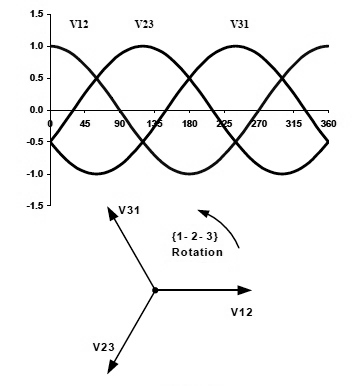
\includegraphics[width=\textwidth]{Unblance_EPS_Pics/Three-phase-voltage-system_gray.png}
         \caption{Three phase sine wave of network voltage.}
         \label{BASICUNB:fig:UnbWave}
     \end{subfigure}
		\hfill
     \begin{subfigure}[b]{0.49\textwidth}
         \centering
         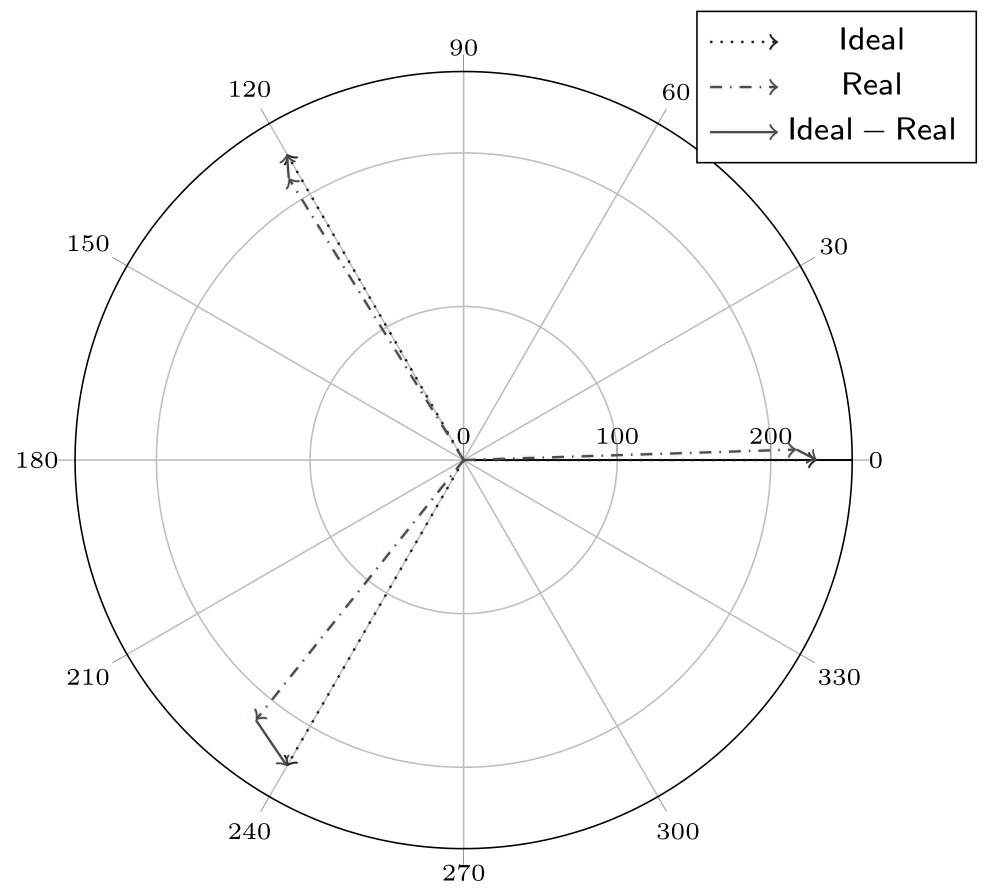
\includegraphics[width=\textwidth]{Unblance_EPS_Pics/PhasorGrayscale.jpg}
         \caption{The three phase voltage phasor whith $Ideal$ and $Real$ voltage vectors.}
         \label{BASICUNB:fig:UnbPhasor}
     \end{subfigure}
        %\caption{BASICUNB:fig:UnbPhasor}
        \label{BASICUNB:fig:UnbPhasor_all}
\end{figure}
	
	This is observed as a frequently cited power quality issue in low-voltage domestic distribution networks and in systems that supply large single phase loads distributed unevenly among the phases. Effects of voltage unbalance are complex, but can be categorized as structural or functional. The former refers to the asymmetry in the three-phase impedances of transmission lines, cables, transformers, etc. It occurs because it is neither economical nor necessary to maintain distribution system with perfectly symmetrical impedances. The latter refers to uneven distribution of power consumption over the three phases. Although the term voltage unbalance is unambiguous, the root phenomenon may be various as well as the standard norms used to measure unbalance. All of these different indicators measure voltage unbalance but each of them does it in a different way. In this section a detailed explanation is presented about the types of currently used method for indication.
	
	\subsection{Types of voltage deviations and norms}\label{BASICUNB:sec:DefinitionsofUNB}

        Voltage unbalance is not a straightforward term. To understand the concept, unbalance is when on a given frequency (mostly fundamental frequency) voltage vectors (phase or line depending on the definition) deviating from the ideal in terms of length or angle. The first fall in to the category of unbalance, namely any kind of phase deviations, and unbalanced amplitude deviations, and balanced amplitude deviations, like under-voltage. There are many different technological causes with more or less practical importance. The following conditions are examined and tested in the sequel:
        \begin{description}
        \item[Single phase under-voltage unbalance]  If there is a single phase uncompensated overload in the system, the voltage in the overloaded phase will be lower than the other two.
        \item[Two phase under-voltage unbalance]  Two of the three phases are overloaded without compensation, the two overloaded phases will have higher voltage drop than the third phase.
        Balanced three phase under-voltage]  The loads of all three phases are overloaded in an unbalanced manner.
        \item[Unbalanced single phase angle]  If the three phase voltage amplitudes are balanced but the relative angles between them (ideally it should be equal to $\pm120$ degree). It is assumed, that $V_a$ would be the reference. If one of the other two phase angles is deflected, unequal displacement.
        \item[Unbalanced two phase angles displacement] Similar to the single phase angle unbalance, if the other two phase angles are both deflected, then unequal angle displacement in two phase angles occurs.
        \end{description}
        An indicator of the voltage unbalance is supposed to measure the extent of unbalance but it is not expected to classify between the above types.
	
	\subsection{Non standardized approximation formulas}\label{BASICUNB:sec:ApproxFormula}
	
	Up to now, the following definitions have not been adopted by any standard or rule to indicate the degree of voltage unbalance, but used by various manufacturers. Firstly based on \cite{eugene1986new} recommended by the CIGRE (International Council on Large Electric Systems, in French: Conseil International des Grands Réseaux Électriques), the voltage unbalance is determined with:
	
	\begin{equation}
        \begin{array}{rcl}
            VUFactor&=&\frac{\sqrt{{1-\sqrt{3-6\frac{V_{ab}^4+V_{bc}^4+V_{ca}^4}{\left(V_{ab}^2+V_{bc}^2+V_{ca}^2\right)^2}}}}}{1+\sqrt{3-6\frac{V_{ab}^4+V_{bc}^4+V_{ca}^4}{\left(V_{ab}^2+V_{bc}^2+V_{ca}^2\right)^2}}}\\
						%\textnormal{where},&&\\
						%\upsilon&=&\frac{V_{ab}^4+V_{bc}^4+V_{ca}^4}{\left(V_{ab}^2+V_{bc}^2+V_{ca}^2\right)^2},					
        \end{array}
        \label{BASICUNB:equ:CIRGE}
    \end{equation}
		
		where, $\{V_{ab},V_{bc},V_{ca}\}$ are the line-to-line voltages. Note, that the CIRGE variant has no distinct notation, as such it would be indicated as $VUFactor$ in this thesis. Moreover, the author of \cite{robert1992assessing} recommends two more variants, based on manufacturer recommended"standards":
		
		\begin{equation}
        \begin{array}{rcl}
            VU&=&\frac{82\cdot\sqrt{(V_{ab}-V_{avg_{line}})^2+(V_{bc}-V_{avg_{line}})^2+(V_{ca}-V_{avg_{line}})^2}}{V_{avg_{line}}}\times100\\					
        \end{array}
        \label{BASICUNB:equ:VU}
    \end{equation}
		
		\begin{equation}
        \begin{array}{rcl}
            VUR&=&\frac{max\left( |V_{ab}-V_{bc}|,|V_{bc}-V_{ca}|,|V_{ca}-V_{ab}| \right)}{V_{avg_{line}}}\times100,\\				
        \end{array}
        \label{BASICUNB:equ:VUR}
    \end{equation}
		
		where the mean of line voltages is noted by $V_{avg_{line}}=\frac{V_{ab}+V_{bc}+V_{ca}}{3}$.
		This formulas were created with the intention to avoid the use of the complex algebra in symmetrical components and give
a good approximation of the later described $VUF$ standard. With the indicator of \ref{BASICUNB:equ:VU}, and as well as \ref{BASICUNB:equ:VUR}. It is worth noticing, that only the voltage magnitude unbalance is reflected, completely ignoring Fortescue's method of symmetrical components \cite{fortescue1918method} (shall presented later in the thesis), which considers negative sequence components as harmful on electric equipment and yield. Later it will be shown that other methods try to push the same methodology, until the currently used norm ($VUF$) is used.

	
	\subsection{LVUR}\label{BASICUNB:sec:LVUR}
	
	One of the first voltage unbalance in percent is defined by the National Electrical Manufacturers Association (NEMA) \cite{bonnett1997understanding} is defined  as the ratio of the maximum voltage deviation from the average line voltage magnitude to the average line-voltage magnitude.
	
\begin{equation}
        \begin{array}{rcl}
            LVUR&=&\frac{\max\left( |V_{ab}-V_{avg_{line}}|,|V_{bc}-V_{avg_{line}}|,|V_{ca}-V_{avg_{line}}| \right)}{V_{avg_{line}}}\times100\\			
        \end{array}
        \label{BASICUNB:equ:LVUR}
    \end{equation}
		
		The LVUR assumes that the average voltage is always equal to the rated value, which is 480 volts for the US three-phase systems, and it works only with magnitudes. Phase angles are not considered in this definition.
	
	\subsection{PVUR}\label{BASICUNB:sec:PVUR}
	
	The next phase voltage unbalance in percent described in IEEE standard $141.$ \cite{IEEE_141_35071} (derived from \cite{IEEE_112_8635630}), is $PVUR_{IEEE-141}$. It is defined as the ratio of the maximum voltage deviation of phase voltages from the average phase-voltage magnitude to the average phase voltage magnitude. In various fields, LVUR and $PVUR_{IEEE-141}$ are commonly used to estimate the degree of voltage unbalance due to simplicity of calculation. The two unbalance factors mentioned above cannot completely reflect system voltage unbalance effects, such as the phase displacements of unbalanced voltages.
	
	\begin{equation}
        \begin{array}{rcl}
            PVUR_{IEEE-141}&=&\frac{\max\left( |V_{a}-V_{avg_{phase}}|,|V_{b}-V_{avg_{phase}}|,|V_{c}-V_{avg_{phase}}| \right)}{V_{avg_{phase}}}\times100,\\
        \end{array}
        \label{BASICUNB:equ:PVUR-141}
    \end{equation}

where the voltages $\{V_{a},V_{b},V_{c}\}$ denotes the phase-to-neutral voltages, and $V_{avg_{phase}}=\frac{V_{a}+V_{b}+V_{c}}{3}$.
The second variant is, $PVUR_{IEEE-936}$, mentioned in \cite{IEEE_936_29053} is defined as the ratio of the difference between the highest and the lowest phase-voltage magnitude to the average phase-voltage magnitude. Therefore, the numerical values of voltage balance quantified by $PVUR_{IEEE-936}$ are generally larger than those of $PVUR_{IEEE-141}$ and LVUR.

\begin{equation}
        \begin{array}{rcl}
            PVUR_{IEEE-936}&=&\frac{\max\left( |V_a|,|V_b|,|V_c| \right)-min\left( |V_a|,|V_b|,|V_c| \right)}{V_{avg_{phase}}}\times100,\\					
        \end{array}
        \label{BASICUNB:equ:PVUR-936}
    \end{equation}
		
The number of possible combinations of three phase or line voltages that satisfy the definitions of voltage unbalance mentioned above will become infinite as only the magnitudes of voltages are considered.	
		
	
	\subsection{VUF and CVUF}\label{BASICUNB:sec:VUFCVUF}
	
	The voltage unbalance factor ($VUF$) was defined by the International Electrotechnical Commission \cite{pillay2001definitions}, \cite{dugan1996electrical}. From the theorem of symmetrical components \cite{fortescue1918method}, voltage unbalance can be considered as a phenomenon that positive sequence voltage  ($V_p$) is disturbed by negative  ($V_n$) and zero-sequence ($V_0$) voltages:
	
	\begin{equation}
        \begin{array}{rcl}
            \begin{bmatrix}
						V_0\\
						V_p\\
						V_n\\
						\end{bmatrix}&=&
						\frac{1}{3}\begin{bmatrix}
						1&1&1\\
						1&\upsilon&\upsilon^2\\
						1&\upsilon^2&\upsilon\\
						\end{bmatrix}\cdot
						\begin{bmatrix}
						V_a\\
						V_b\\
						V_c\\
						\end{bmatrix},\\
        \end{array}
        \label{BASICUNB:equ:symmetry}
    \end{equation}
	
	Where $\upsilon=e^{2j\pi/3}$ is the Fortesque operator. From that the formula of $VUF$ can be expressed as:
	
	
	\begin{equation}
        \begin{array}{rcl}
            VUF&=&\left|\frac{V_n}{V_p}\right|\times100,\\					
        \end{array}
        \label{BASICUNB:equ:VUF}
    \end{equation}

    \begin{figure}[h]
         \centering
         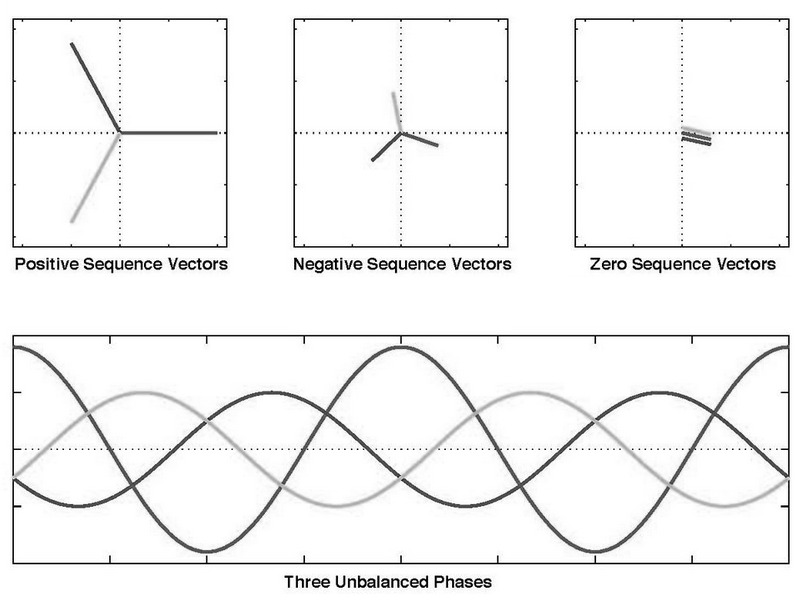
\includegraphics[width=.7\textwidth]{Unblance_EPS_Pics/Symmetrical_components_gray.jpg}
         \caption{Simplified graphical display of symmetrical components.}
         \label{BASICUNB:fig:symmetrical_simple}
     \end{figure}
	
This norm is currently in use world wide for voltage unbalance indication. The main focus in on the negative sequence component $V_n$, on which many studies attributes importance of the cause of negative effects the voltage unbalance causes.\\
	As such, three-phase electric loads without path through the neutral, negative-sequence voltage is the primary cause of voltage unbalance. Normally, positive-sequence component of three-phase voltages is very close to rated value. If expressed in per-unit quantities, the positive-sequence voltage will be very close to $1.0$ p.u., and the corresponding negative-sequence voltage will be very close to the $VUF$. Thus, the $VUF$ can indeed be considered as the negative-sequence component in per-unit.	This explains the advantage of using the VUF as an index for analyzing the effects of voltage unbalance considering the phase deviations.
	An extension of the VUF is the complex voltage unbalance factor ($CVUF$) that is defined by the ratio of the negative-
sequence voltage phasor to the positive-sequence voltage phasor studied in \cite{wang2000analytical}, and \cite{pierrat1987unbalance}. The CVUF is a complex quantity having the magnitude and the angle. Although the CVUF has not yet been widely used by practicing engineers, it has been proposed in some studies (e.g., \cite{wang2001analysis}, \cite{singh2007some}, \cite{chen2013examination}) due to its richness of information on unbalance. The formula of $CVUF$ is similar to $VUF$:

\begin{equation}
        \begin{array}{rcl}
            k_v&=&\frac{V_n}{V_p}=k_v\cdot e^{j\theta_v}=k_v\angle\theta_v,\\					
        \end{array}
        \label{BASICUNB:equ:CVUF}
    \end{equation}
		
		where $k_v$ is the magnitude and $\theta_v$ is the angle of $CVUF$.
		
			It can be observed, that the previously mentioned norms \ref{BASICUNB:equ:CIRGE}, \ref{BASICUNB:equ:VU}, \ref{BASICUNB:equ:VUR}, \ref{BASICUNB:equ:LVUR}, \ref{BASICUNB:equ:PVUR-141}, \ref{BASICUNB:equ:PVUR-936}, and \ref{BASICUNB:equ:VUF}  indicate different values for a single case with various correlations. The first two standard indicators, $PVUR_{IEEE-936}$ and $PVUR_{IEEE-141}$, ignore the $\pm120$ degree phase difference unbalance and only take the amplitudes into account. Additionaly, the zero-sequence components never present in the line-to-tine voltages regardless of the level of unbalance, only phase-to-neutral voltages. It has been proven, that these components are unelectable in some cases like bridge control of converters \cite{betz2006symmetry}, or synchronous machine diagnosis \cite{hang2015online}.\\
			The actual state of the art definition in use, $VUF$, is sensitive to the phase difference unbalance. Lastly $CVUF$ considers also phase and magnitude of the voltage unbalance, but the two units are hard to merge together as the optimization cost of a cost function. Moreover, these definitions ignore zero sequence components and harmonic distortion that are always present in three-phase four-wire systems \cite{bina2011three}.
		
% =========== SECTION MIGRATED TO INTRODUCTION -->

			%\section{Effects of voltage unbalance}
			%
			%Many power systems, voltage parameters change over time. Variation of power quality disturbances leads to thermal transients in electrical machines. This problem can be especially important in the case of low-power machines, because they have shorter time constants than high-power ones. The rate of thermal responses of a machine also significantly depends on the type of power quality disturbances. Voltage unbalance can cause  machine  overheating  within  a  mere  few  minutes. Furthermore,  fluctuating  unbalance  could  cause  an  extraordinary rise  in  windings  temperature  and  additional  thermo-mechanical stress.  Consequently,  voltage  unbalance  is  found  to  be  more harmful to induction motors than the results from previous works \cite{gnacinski2019induction}. Additionally beside the heat factor, voltage unbalance can cause increased reactive power \cite{savaghebi2012secondary}, various copper loss \cite{siddique2004effects} torque pulsation in electric motors \cite{brekken2005control} have been studied.

\section{Proposed geometrical indicator}\label{VUB:sec:Geom}

As discussed in section \oldref{BASICUNB:sec:DefinitionsofUNB}, the indicators of voltage unbalance result very different measures for the same circumstance. Additionally most of them are neglecting the phase differences of voltage vectors compared to the ideal, and even the currently used $VUF$ calculated by \ref{BASICUNB:equ:VUF} is not taking zero sequence components from the Foresque method \cite{fortescue1918method}. There were attepts to close the gap with the CVUF norm shown in \ref{BASICUNB:equ:CVUF}, where the complex component is also considered, but this makes this a clumsy candidate for control design, since two components (real and complex part) shall be weighted and applied. This begs the question, how could voltage unbalance be measured loss-less, but resulting one (conveniently quadratic-like) value, easily applicable for optimization algorithm. \\
Hence can be stated that every difference between the ideal and the measured voltage in both amplitude phase and sub-harmonics causing a form of voltage deviation. The problem can also be investigated from a geometrical point of view as it is depicted in Figure \ref{fig:threephase}. The three-phase voltage system's phasor diagram contains three  phase-to-neutral voltage vectors which can be regarded as the points of a triangle (similarly, the three line-to-line vectors can play the role of the edges of the triangle). The two triangles (i.e. the ideal and the actual ones) always intersect except from very extreme and physically meaningless cases. The area where the two triangles do not cover each other (i.e. the difference of their union and intersection) can be used as a norm of voltage quality. In fact it is computationally more demanding compared to the previous methods, but takes every deviation into consideration \cite{Neukirchner2015},\cite{neukirchner2015examination}. The calculation of error is given by \ref{equ:geom}.

            \begin{equation}
                \begin{array}{rcl}
                       G&=&\textnormal{Area of }(\bigtriangleup_{Ideal}\cup\bigtriangleup_{Real}-\bigtriangleup_{Ideal}\cap\bigtriangleup_{Real}),
                \end{array}
                \label{equ:geom}
            \end{equation}

            $\bigtriangleup_{Ideal}$ indicates the triangle spanned by the ideal voltage vectors and $\bigtriangleup_{Real}$ the triangle of real voltage vectors. Difference of the ideal and the real triangle's union and intersection defines the norm $G$. Basically, the algorithm calculates the symmetrical difference of the triangles, stretched from three phase ideal and real voltage vectors.

            \begin{figure}[!ht]
           \centering
           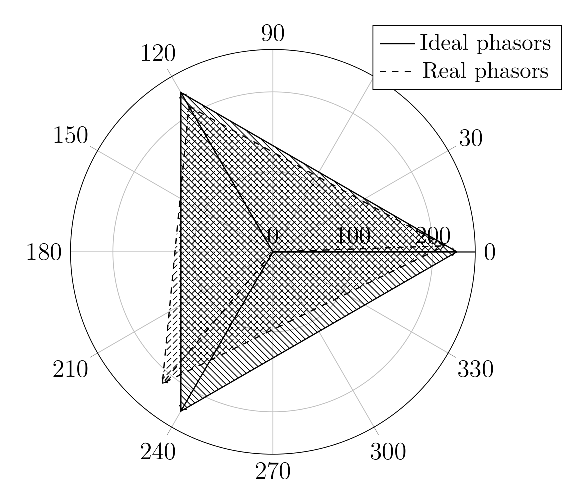
\includegraphics[scale=0.95]{Unblance_EPS_Pics/UnbalRedComp_JCP-figure1.eps}
           \caption{The triangles spanned by the ideal and the actual voltage phasors. The extent of voltage deviation on the network can be measured by the sum of areas where the two triangles are not overlapping.}
           \label{fig:threephase}
            \end{figure}

\section{The method's novelty compared to VUF}\label{VUB:sec:AdditionalContent}

When using a new norm for calculation and cost function it is reasonable to test it's usability against the prevalent or regulated method the voltage unbalance factor ($VUF$) defined by the International Electrotechnical Commission, as discussed in section \oldref{BASICUNB:sec:VUFCVUF}. In this case the geometrical norm's utility \ref{equ:geom} against the $VUF$ value shall be examined. \\
The geometrical norm was validated experimentally, by investigating the correlation between the regulated  and geometrical norms subjected to random, uniformly distributed unbalance on the voltage vector amplitude and phase values with $20$ V amplitude and $1/300\cdot\pi$ rad phase variance (Fig. \ref{fig:correlation}, and Fig. \ref{fig:side_correlation}).

            \begin{figure}[!ht]
           \centering
           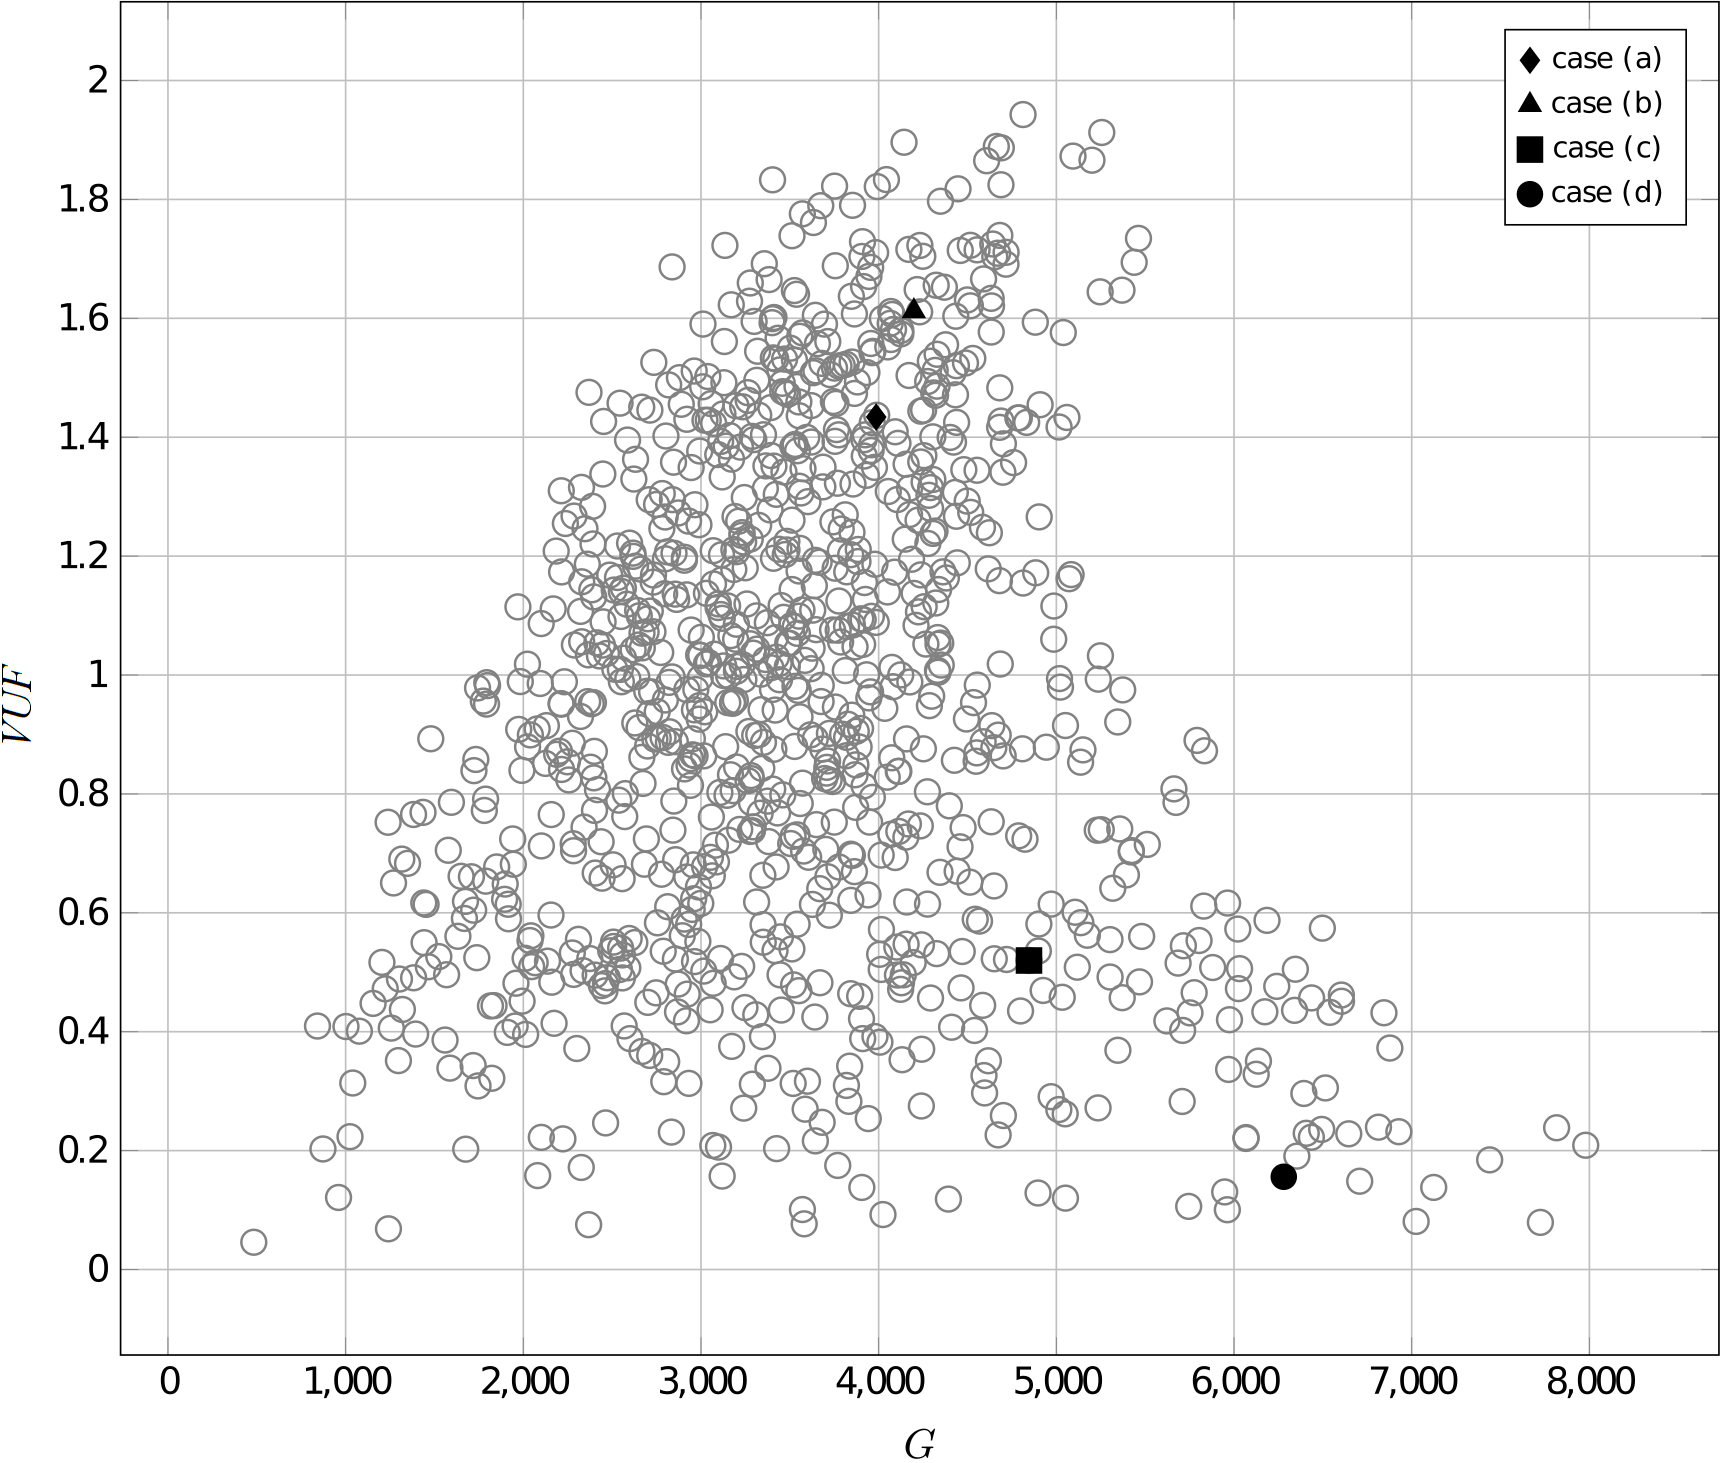
\includegraphics[width=\textwidth,scale=0.95]{Unblance_EPS_Pics/EPS_images/scatter.png}
           \caption{Correlation between the geometrical voltage unbalance indicator $G$ and the regulated voltage unbalance indicator $VUF$ using 1000 samples. In every iteration each three phase voltage vector's amplitude and phase values changed randomly, according to uniform distributions with $\pm20$ V amplitude and $\pm\frac{1}{3}\pi\cdot10^{-2}$ rad phase variance. It can be seen, that the geometric norm contains more information than the classical one. The  four asymmetry cases of Figure \ref{fig:cases} are denoted by black symbols on the picture. It is apparent, that in case (c), and (d) the G norm holds additional information than the $VUF$.}
           \label{fig:correlation}
            \end{figure}

            \begin{figure}[!ht]
           \centering
           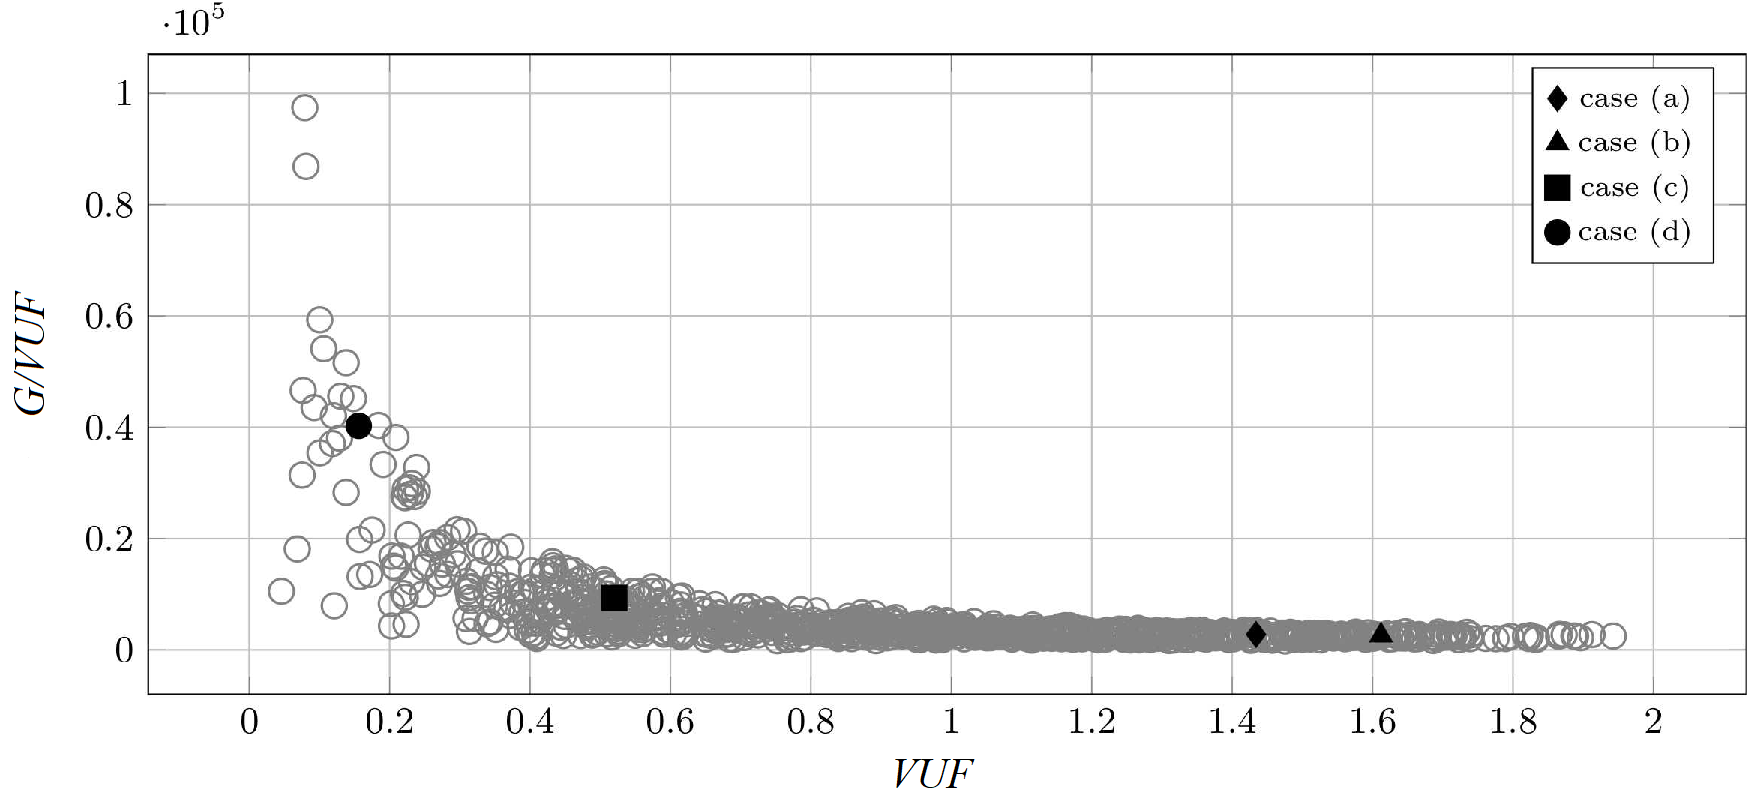
\includegraphics[width=\textwidth,scale=0.95]{Unblance_EPS_Pics/EPS_images/side_scatter.png}
           \caption{ Correlation between the regulated unbalance indicator and the fraction of geometrical and regulated indicator. It can be seen that there is a functional connection between the two values.}
           \label{fig:side_correlation}
            \end{figure}


            Although there is correlation between the two norm values in the general case, but for some situations the regular method indicates low, while geometrical norm still indicates high value.\\
            On Figure \ref{fig:cases_A} dominant phase deviation can be observed, while Figure \ref{fig:cases_B} shows amplitude deviation but with opposite direction. When there is such deviation on the grid both indicators present almost identical results. On \ref{fig:cases_C} there is still observable unbalance (two phase deviate stronger than the third in terms of amplitude), but the correlation is significantly lower. In the last case in the lowest correlation area, amplitude deviation is present, but the deviation direction is identical on all phases (balanced over-voltage or under-voltage, can be observed on Figure \ref{fig:cases_D}). The regular method indicates very low values. In this case other methods are utilised in parallel in terms of network diagnostics to detect the under-voltage phenomena.\cite{arn1997under-voltage}.


            \begin{figure}
                \centering
                \begin{subfigure}[b]{0.48\textwidth}
                    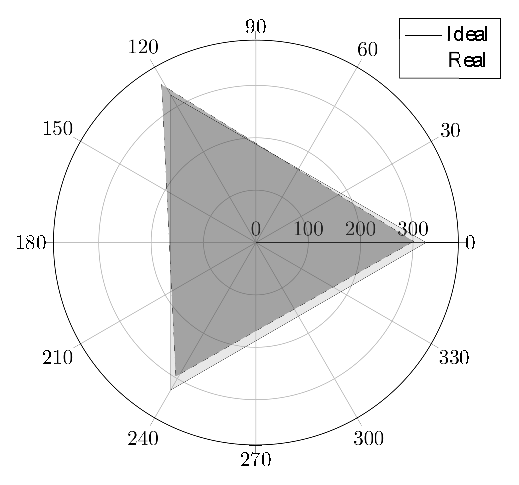
\includegraphics[width=\textwidth]{Unblance_EPS_Pics/EPS_images/rombus.eps}
                    \caption{\centering High correlation with phase deviation. The norm values are $G=3986$ and $VUF=1.434$.}
                    \label{fig:cases_A}
                \end{subfigure}
                ~ %add desired spacing between images, e. g. ~, \quad, \qquad, \hfill etc.
                  %(or a blank line to force the subfigure onto a new line)
                \begin{subfigure}[b]{0.48\textwidth}
                    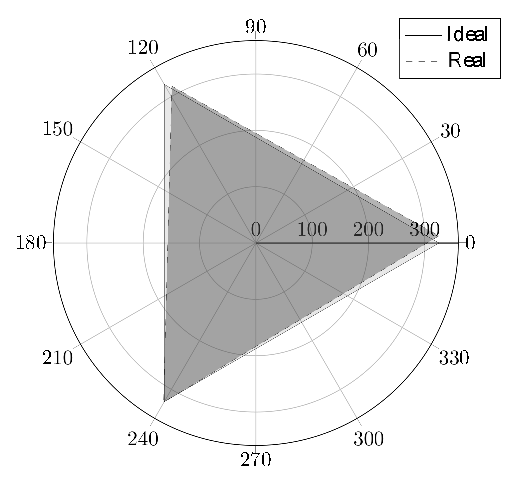
\includegraphics[width=\textwidth]{Unblance_EPS_Pics/EPS_images/triangle.eps}
                    \caption{\centering High correlation with opposed amplitude deviation. The norm values are $G=4198$ and $VUF=1.612$.}
                    \label{fig:cases_B}
                \end{subfigure}
                 %add desired spacing between images, e. g. ~, \quad, \qquad, \hfill etc.
                %(or a blank line to force the subfigure onto a new line)
                \begin{subfigure}[b]{0.48\textwidth}
                    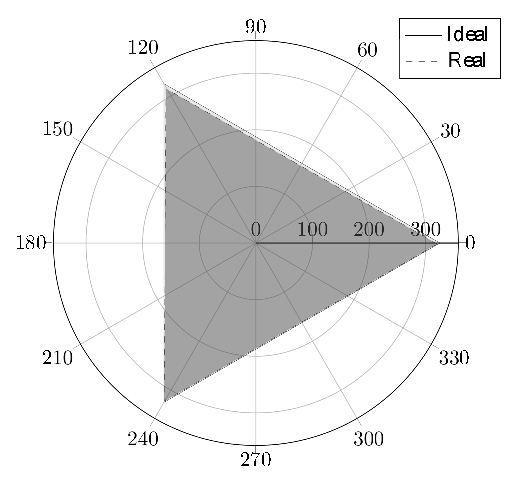
\includegraphics[width=\textwidth]{Unblance_EPS_Pics/EPS_images/square.eps}
                    \caption{Low correlation with opposed amplitude deviation. The norm values are $G=9322$ and $VUF=0.5198$.}
                    \label{fig:cases_C}
                \end{subfigure}
                ~
                \begin{subfigure}[b]{0.48\textwidth}
                    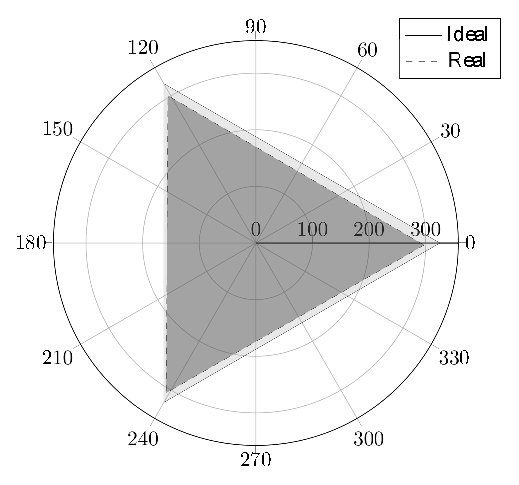
\includegraphics[width=\textwidth]{Unblance_EPS_Pics/EPS_images/circle.eps}
                    \caption{\centering Low correlation with uniform voltage drop. The norm values are $G=6280$ and $VUF=0.156$.}
                    \label{fig:cases_D}
                \end{subfigure}


                \caption{Four distinct cases of voltage triangles examining correlation between the regular $VUF$ and geometrical $G$ method.}\label{fig:cases}
            \end{figure}

To clarify this, the regular norm's calculation method needs to be investigated. The symmetrical component mutual impedance matrix on a three phase connection point is given by \ref{equ:mutual},

            \begin{equation}
                \begin{array}{rcl}
                       Z_s&=&\frac{1}{3}\begin{bmatrix} 1&1&1\\1&\alpha&\alpha^2\\1&\alpha^2&\alpha \end{bmatrix}\cdot
                                        \begin{bmatrix} Z_{aa}&Z_{ab}&Z_{ac}\\Z_{ba}&Z_{bb}&Z_{bc}\\Z_{ca}&Z_{cb}&Z_{cc} \end{bmatrix}\cdot
                                        \begin{bmatrix} 1&1&1\\1&\alpha^2&\alpha\\1&\alpha&\alpha^2\end{bmatrix}=\\
                          &=&  \begin{bmatrix} Z_{00}&Z_{01}&Z_{02}\\Z_{10}&Z_{11}&Z_{12}\\Z_{20}&Z_{21}&Z_{22} \end{bmatrix},

                \end{array}
                \label{equ:mutual}
            \end{equation}

where $Z_s$ is the symmetrical component mutual impedance matrix, and $\alpha=e^{j\frac{2}{3}\pi}$. If there are both negative and zero sequence symmetrical components present on the network, the dominant part of the voltage drop's negative and zero sequence can be calculated as follows \ref{equ:drop}.

            \begin{equation}
                \begin{array}{rcl}
                       \Delta U_2&\approx&Z_{21}I_1+Z_{22}I_2\\
                       \Delta U_0&\approx&Z_{01}I_1+Z_{00}I_0,
                \end{array}
                \label{equ:drop}
            \end{equation}

$\Delta U_0,\,\Delta U_1,\,\Delta U_2$ are the voltage drop's zero positive and negative sequence components, $I_0,\,I_1,\,I_2$ are the current's drop's zero positive and negative sequence components, and $Z_{00},Z_{01},\,Z_{21},\,Z_{22}$ are mutual impedances,  respectively. (If there is only positive and negative sequence present, then the right hand side's second term is zero.) As such, the indication of negative and zero sequence present the network calculates \ref{equ:factor}:

            \begin{equation}
                \begin{array}{rcl}
                       m_{21}&=&\mid\frac{Z_{21}}{Z_{11}}\mid\times100\\
                       m_{01}&=&\mid\frac{Z_{01}}{Z_{11}}\mid\times100,
                \end{array}
                \label{equ:factor}
            \end{equation}

where $m_{21}$ is the negative sequence factor which is identical to the $VUF$, and $m_{01}$ is the zero sequence factor.\\
At the previously described balanced over- or under-voltage case the positive sequence value is dominant, so the regular indicator will take considerably lower value. In other words, aside from indicating voltage unbalance, the geometrical method incorporates the balanced deviations as well. In a control design perspective, a general case, where notably highly unbalance values may appear, using $VUF$ as cost function could introduce hidden errors in control due error cancellation. Additionally the geometrical solution checks electrical asymmetry, i.e. the norm of a $\pm120$ degree rotated version of the ideal three-phase phasor is zero in the geometrical sense. Moreover, the geometrical norm is more sensitive for small scale unbalance, as opposed to the $VUF$. To summarize, the geometrical indicator a more suitable solution for a more general case indicator, and a good candidate for cost function in optimal control design.
\newpage
\section*{Notations used in the chapter}

\begin{scriptsize}
\begin{tabularx}{\textwidth}{r|X}
% A
%$\textbf{A}$																& State matrix of a linear time invariant model\\
%$\textbf{A}_x$              & Constraint state matrix\\
%$\textbf{A}_u$              & Constraint input matrix\\
%$\textbf{A}_f$              & Constraint state matrix at the end of the horizon\\
%$\mathcal{A}$               & Set if indices in states where the constraints are active\\
%$\mathcal{A}^N$               & Set if indices in states where the constraints are inactive\\
%
%
%% B
%$\textbf{B}$																& Input matrix of a linear time invariant model\\
%$\textbf{b}_x$              & Constraint state coefficient\\
%$\textbf{b}_u$              & Constraint input coefficient\\
%$\textbf{b}_f$              & Constraint state coefficient at the end of the horizon\\
%
%% C
$CVUF$  													& Complex Voltage Unbalance Factor\\
%$\textbf{C}$																& Output matrix of a linear time invariant model\\
%$C_{snub}$ 												& Capacitance to reduce switching loss and to damp out over-voltage\\
%$C_D$															& Capacitance for filtering the output voltage of the VSR\\
%$C_S$															& Input filter capacitance of the three phase alternating current in CSR\\
%$\mathcal{C}_{\mathcal{A}}$               & Critical region associated with the active constraints\\
%
%% D
%$D_{1+},D_{2+}$										& Higher diodes\\
%$D_{1+},D_{2+}$										& Lower diodes\\
%$d_i$															& Direction of active process\\
%
%% E
%$\textbf{E}$                & Unified constraint state matrix \\
%$\mathcal{E}$               & Set of external sucesses\\
%
%% F
%$\textbf{F}$                & State coefficient matrix for calculating the optimal input \\
%$f(x)$														& Function of the state\\
%
%% G
$G$                               & Geometrical voltage unbalance indicator \\
%$\textbf{G}$                & Unified constraint input matrix \\
%$\mathcal{D}$               & Set of directions\\
%$g$                         & Autonomous function where there are no inputs\\
%$g_l$                       & Equality constraints of a Lagrange function\\
%
%% H
%$\textbf{H}$                & Supplementary quadratic optimizer matrix\\
%$h$                                                             & Transformer turn ratio\\
%
%% I
$I_{0,1,2}$												& Zero positive and negarive sequence of current drop\\	
%$I_D$															& Direct output current\\
%$\mathcal{I}$               & Set if internal sucesses\\
%$\mathcal{I}_c$               & Set if indices of constraints\\
%$i_{abc}$                   & Generic three phase current\\
%$i_i$															& Constant input inductor current\\
%$i_o$															& Alternating output current\\
%$i_{dq0}$                   & Three phase current converted to Park frame\\
%$i_{\alpha\beta\gamma}$                   & Three phase current converted to Clarke frame\\
%$\vec{i}$													& Rectifier input current\\
%$\vec{i}_ref$											& Reference rectifier input current\\
%
%
%% J
%$J_0$                           & Cost (or value) function to optimize at the initial state\\
%$J^*_0$            & Optimal cost value at the initial state\\
%$\mathcal{J}$               & Set if indices of active constraints\\
%
%% K
%$\textbf{K}$                & Controller gain\\
%$\mathcal{K}$               & Set of states respective to constraints\\
%$\mathcal{K}^*$               & Set of feasible states respective to constraints\\
$k_v$  														& Magnitude of CVUF\\
%$k$																& Time step on the horizon $N$ \\
%
%% L
%$L_+,L_-$													& Current filter inductors\\
%$L_a$															& Leakage inductance\\
%$L_S$															& Input filter inductance of the three phase alternating current in VSR\\
%$L_D$															& Inductor for filtering the output current of the CSR (Choke)\\
$LVUR$														& Voltage unbalance notation based on NEMA standard\\
%
%% M
%$m$                             & Dimension of the input vector\\
$m_{21}$                        & negative sequence factor, identical to $VUF$\\
$m_{01}$                        & zero sequence factor\\
%
%
%% N
%$N$											& Defined horizon of MPC\\
%$N_c,N_u,N_y$											& Defined control, input, and output horizon respectively\\
%$n$                             & Dimension of the state vector\\
%
%% O
%
%% P
%$\textbf{P}$                    & Terminal penalising weight matrix\\
%$\mathcal{P}$                   & Set of processes\\
%$\mathcal{P}^c$               & Set of all (input and state) constraints at time instance\\
%$\mathcal{P}_p$             & Set of primary feasibility conditions\\
%$\mathcal{P}_d$             & Set of dual feasibility conditions\\
$PVUR_{IEEE-141},PVUR_{IEEE-936}$	& Voltage unbalance notation based on IEEE-141, and IEEE-936 standard\\
%$p$																& Process number\\
%
%% Q
%$\textbf{Q}$                    & State penalising weight matrix\\
%$\mathcal{Q}$                   & Set of sidestep indices\\
%$q$																& Discrete time step\\
%
%% R
%$\textbf{R}$                    & Input penalising weight matrix\\
%
%% S
%$S_{1+},S_{2+}$										& Higher switches\\
%$S_{1+},S_{2+}$										& Lower switches\\
%$\textbf{S}$              & General state constraint coefficient\\
%$\mathcal{S}$                   & Set of successful iterations\\
%$\mathcal{S}^x$             & Set of all possible future state matrices stepping through the horizon\\
%$\mathcal{S}^u$             & Set of all possible future input matrices stepping through the horizon\\
%$s$                             & Dimension of the decision vector\\
%
%% T
%
%% U
%$\textbf{U}^*_0$            & Optimal vector of future inputs starting from the initial state\\
%$\mathcal{U}$              & Set of unsuccessful steps\\
%$\mathcal{U}^u$             & Set of inputs not violating constraints\\
%$\textbf{u}^*$            & Optimal vector of input\\
%$\widehat{u}$				& Peak value of AC-side capacitor voltage\\
%
%% V
%$V$                         & Lyapunov function\\
$V_{ab},V_{bc},V_{ca}$  					& Line-to-line voltages\\
$V_{avg_{line}}$  								& Average of line voltages\\	
$V_{a},V_{b},V_{c}$  							& Phase-to-neutral voltages\\
%$V_{an},V_{bn}$  									& Designated point's potential to ground \\
$V_{avg_{phase}}$  								& Average of phase voltages\\
%$V_i$															& Constant input voltage\\
%$V_o$															& Alternating output voltage\\
$V_{0},V_{p},V_{n}$  							& Zero, negative and positive sequence voltages based on symmetrical components theorem\\
%$V_{D1},V_{D2}$ 									& Two end's voltage on the DC-DC converter\\
%$V_d$															& Output voltage\\
$\hat{V}$															& Voltage peak\\
$\vec{V}_a, \vec{V}_b, \vec{V}_c,$										& Voltage vectors in the three phase phasor\\
$VUF$  														& Voltage Unbalance Factor\\
$VUFactor,VU,VUR$                	& Non standardized voltage unbalance factor based on manufacturer standards\\
%$v_{c_p}$													& AC-side capacitor voltage, where $p\in\{1,2,3\}$\\
%$v_1,v_2$                         & Transformer voltages\\
%$v_D$															& Output voltage before the choke inductor $L_D$\\
%$v_{i,j}$													& Three phase phase-to-neutral voltage $i,j\in\{R,S,T\}$\\
%$v_{N,RS}$												& Three phase line-to-line voltage of $R$ and $S$\\
%
%% W
%$\textbf{w}$                & Unified constraint vector \\
%
%% X
%$\mathcal{X}^x$             & Set of all possible future states stepping through the horizon\\
%$\textbf{x}$											& State vector of a linear time invariant model\\
%$\bar{\textbf{x}}$											& Minimum state value of the objective function\\
%$\textbf{x}(0)$                 & Initial state\\
%$x_i^{best}$											& Best reached state, where $x_i^{best}$ is a minima\\
%
%% Y
% $\textbf{Y}$ & Supplementary matrices\\
%
%% Z
$Z$												& Symmetrical component mutual impedance\\
%$\textbf{Z}^*$              & Set of optimizers leading to feasible states\\
%$\textbf{z}$											& Optimizer of linear multi parametric problem\\
%$\tilde{\textbf{z}}$        & Set of all future states and inputs over the horizon\\
%
%% Greek
$\Delta U$													& Zero positive and negative sequence of voltage drop\\
%$\Delta$													& Step length control parameter\\
%$\Delta_i^{best}$											& Best reached step size\\
$\theta$                    & Angular displacement of the voltage or current vector\\
$\theta_v$  											& Angle of CVUF\\
%$\lambda$                   & Lagrange multiplier\\
%$\nu_i(q)$ 												& Time index for the completion of the function evaluation that produced the update at time step $q$ on process $i$\\
%$\rho$																& Infinite sequence iterator\\
%$\varphi_N$												& Angle of phase voltage\\
$\upsilon$  											& Fortesque operator\\
%$\tau_i(q)$												& Time index for initialization of the function evaluation, that produced the update at time $q$ on process $i$\\
%$\omega$													& Angular velocity of output sinusoidal voltage or current\\
%$\omega_i(q)$ 										& Generating process index for the update time at step $q$ on process $i$\\

%================================================
\end{tabularx}
\end{scriptsize}



%% Unbalance Compensation
\chapter[Voltage unbalance compensation]{Voltage unbalance compensation with geometrical indicator on a domestic low voltage network}\label{BASIC:sec:unbalance_compensation}

\section{Literature overview}
%============ Network properties and uncertainties
% MonteCarlo
\hlc[MA]{The phenomena of voltage unbalance (VU)}\hlc[PT]{ was investigated for a long time. VU of three-phase voltages results from asymmetry of line impedances and from inequality of loads in three phase networks. Efforts are in general are made to reduce the asymmetry, sprouting form network topology geometries impedance by transposition. On the other hand, voltage unbalance caused by uneven distribution of loads over three phases is more difficult to compensate. In low voltage residential and/or commercial systems, single-phase loads account for the majority of power consumption. Wherever possible,efforts are made to distribute the single phase loads uniformly over three phases, but residential areas are generally not sanctioned per household. It is unlikely that at a given instant loads in the three phases are balanced because they vary in a random manner. In other words, even if the average loads in the three phases are kept the same, the instantaneous power demands in the three phases differ from each other, leading to unbalanced voltages at the point of common coupling. With this in mind, predictive models can not reliably established, however stochastic models has been tried to aid the effort. In} \cite{wang2001method}\hlc[PT]{ a distribution networks were examined, and a Monte Carlo analysis with random variation of the voltage unbalance factor is modeled with the aid of correlated Gaussian random variables that represent random variations in three-phase active and reactive powers. Also this method used in} \cite{schwanz2016stochastic} and \cite{schwanz2016stochastic}, \hlc[PT]{for single phase power plants (mainly PV plants) caused VU risk assessment and mitigation. It was shown that this unchecked plants can cause serious risk with above $2\%$ VUF, and the maximum single-phase and uncontrolled connection of plants is unacceptably high, posing a risk for other networks as well.}\\
% Covariance + neural
\hlc[PT]{The authors of }\cite{xu2018stochastic}\hlc[PT]{ proposed a stochastic multi-objective optimization to model VU, where the discrete decision variables are coordinated with continuous regulation of solar reactive outputs updating they assumed covariances. For the purpose, the stochastic processes of solar active power are modelled in a scenario based framework. Stochastic processes were converted into a series of equivalent deterministic scenarios. For this purpose, a modified non-dominated sorting genetic algorithm-II was proposed, in which crossover rate and mutation rate are dynamically revised by a fuzzy logic controller.}\\
%============ UNBALANCE COMPENSATION
\hlc[PT]{There are different approaches of lowering the unbalance with different control techniques. Since conventional inverter topologies ar built for symmetrical, and zero offset current and voltage waveforms, the topology needed to change, to compensate the negative (and occasionally zero) sequence symmetrical components, besides normal operation. An interesting approach by} \cite{li2005microgrid} \hlc[PT]{was introduced, where two parallel VSIs are connected to produce positive and negative sequence components side by side. The approach also utilizes optimal control to achieve both the quality of power (MPPT) within the microgrid and the quality of currents (unbalance mitigation with low THD) flowing between the microgrid and the utility system, where two parts are controlled complementarily to inject negative- and zero-sequence currents in series to balance the line currents, while
generating zero real and reactive power. An other approach, is to try to estimate the required compensation geometrically by} \cite{lee2009new}, \hlc[PT]{where the required step in space vector modulation (SVM) is calculated by giving the assumed vectorial sum to move the measured system to a more balanced state. The authors use a series connected VSI (with common DC link) to achieve the required freedom for the operation, although the unbalance reduction is for the controlled three phase loads only, and the network is not influenced.\\
In the market there are devices with the sole purpose of compensation, and one of them is the static var compensator (SVC). This device is connected parallel, to the network (usually after the transformer station) to adaptively reduce the networks reactive power. However in} \cite{xu2010voltage} \hlc[PT]{the SVC is used also for mitigating the grid's VU. In the article, as three-phase IGBT-based static synchronous compensator was proposed for voltage and/or current unbalance compensation, where an instantaneous power theory (IPT) was used for real-time calculation and control. This control approach calculates the controller's next step from the instantaneous values of voltage and current to formulate the required power to inject in an averaged time interval.\\
In some cases the authors aim not to reduce the effect of unbalance on the network, but to ensure stable operation, while devices and loads are protected. In} \cite{vekhande2015control} \hlc[PT]{the authors argue, that working under network VU, a current source inverter (CSI) holds a better strategy, than its counterpart, although the device is only operates under this condition and does not contribute to the unbalance even further. The device stands as gateway between a DC microgrid and an AC grid. Under the effect of VU the DC microgrid suffers harmonic oscillations in voltage, and possible controller tripping (one phase exceeds the current limit) if it is not mitigated. The authors mention the use of conventional VSI based structures for CSI may lead to unstable operation, as such, they inject balanced three phase currents into the AC grid under an unbalanced grid voltage. Based on the instantaneous active power theory under unbalanced  grid conditions} \cite{wang2016dc} \hlc[PT]{proposes an optimized negative-sequence current references for  eliminating the double-frequency oscillations on active power at AC side of a current source converter. The approach is similar as before, using CSI as a good topology candidate, as well as the control structure of IPT, but the goal here is also to work under unbalanced grid conditions, and only protecting the device and the load. In} \cite{guo2018advanced} \hlc[PT]{direct control strategy with CSI model based control is shown which is simpler than the complicated IPT. The factors of unbalance are measured (negative and zero sequence as well) and the optimal current is calculated from the device model and from the factors via phase locked loop.\\
As an issue both} {\cite{Hu2016264}, and \cite{el2016control} \hlc[PT]{names the increasing PV penetration a thread for the network quality, namely the voltage balance. The former suggests that the network operators are  mainly obligated to mitigate the phenomena, by the transmission systems management and control, and the former suggests a local strategy. The idea is to use the PV-VSI (voltage source inver with photovoltaic source on the DC end) as the control reserve for VU mitigation. Here also geometrical approach is used with SVI to calculate the VSI's next step and formulate the optimal voltage vector on the voltage phasor, and an intermediate PI controller to reduce parameter sensitivity. The controller's cost function is derived via current and voltage measurement based on the IPT.\\
In this dissertation the approach is, that the low voltage network's level of unbalance only depends on the habits of household residents, as such it is assumed, that the network beyond the connection point is unknown (the amount, type and power of domestic loads are unknown), and network impedance's stochastic distribution function can not be estimated as it shall be discussed in section }\oldref{VUB:sec:Statement}\hlc[PT]{. This implies, that the compensation's goal is to find the local optimum regardless of unknown conditions. Furthermore, the goal is to compensate the VU, without the option to place current controllers after the connection point. This implies, that the grid's transformer's current can not be measured, to esteem the network's behaviour. With this in mind,} in section \oldref{VUB:sec:Optimization} \hlc[PT]{ a control strategy was chosen, which was adequate for said conditions, and searches for the optimum without the necessity of knowing the control gradients. The authors in }\cite{dash2011dynamic} \hlc[PT]{suggest, that current control strategies, where non harmonic currents were used deemed to have difficulties, however the CSI exhibits higher reliability and power density than the VSC with added DC-DC boost converter topology. As such a current source based strategy with only harmonic currents were used, which shall be presented in section} \oldref{VUB:sec:Inverter}.
%%
%Additionally, new computationally efficient control techniques have been presented by \cite{lee2009new} to estimate and compensate input voltage unbalance (VU) disturbances for a voltage source converter. These tools are designed to be effective with high power systems with slower PWM switching frequencies of 5 kHz or lower and limited current-controller bandwidth. About the unbalance compensation control aspect, a three-phase IGBT-based static synchronous compensator were proposed for voltage and/or current unbalance compensation by \cite{xu2010voltage}. An instantaneous power theory was used for real-time calculation and control. Three control schemes current control, voltage control and integrated control were proposed to compensate unbalanced voltage, unbalanced current or both. Unbalance phenomena and power quality can be examined with modeling too. A particular modeling method was presented by \cite{li2005microgrid}, where a three-phase four-wire grid-interfacing power quality compensator were modeled. During voltage unbalance, the compensator, used a shunt with a series four phase inverter, could enhance both the quality of power within the microgrid and the quality of currents flowing between the microgrid and utility system. In this case a microgrid is a group of interconnected loads and distributed energy resources within clearly defined electrical boundaries that acts as a single controllable entity with respect to the grid. A microgrid can connect and disconnect from the grid to enable it to operate in both grid-connected or island-mode. The shunt four-leg inverter were controlled to maintain a set of balanced distortion free voltages to regulate power sharing among the parallel-connected distributed generation systems. Simulation studies were carried out by \cite{Hu2016264} where one of the aims was to develop and test the feasibility of a decoupled three-phase on-load tap charger in the distribution system with the objective of improving the distribution network power quality. Further control methods were applied for the solution for balancing of the most sensitive with regard to electric energy quality part of power system by \cite{korovkin2016uimethod}, minimizing the active power losses, stabilization of three-phase voltages, enhancement of asynchronous machine performance stability and reduction of errors occurring in power consumption measuring circuits.\\
%%============ UNBALANCE COMPENSATION WITH OF CURRENT SOURCE CONVERTERS
%In the arsenal of voltage unbalance compensation, current source power electronic devices have a dedicated position. Based on the instantaneous active power theory under unbalanced  grid conditions \cite{wang2016dc} proposes an optimized negative-sequence current  references  for  eliminating  the double-frequency  oscillations  on  active  power  at  AC  side of a current source converter. The author argues in \cite{wang2014virtual} that a classification of the virtual impedances can greatly benefit an unbalance compensating control structure, with an active stabilization method. In \cite{guo2018advanced} direct control strategy with detailed current converter model is shown which is much simpler than the complicated instantaneous power theory approach. This solution needs less voltage and current sensors for the feedback control, which means that it is a cost-effective solution. An interesting, yet similar approach compared in the paper if a bi-directional current source topology is used like in \cite{vekhande2015control}. This enables to compensate a much larger degree of freedom handing unbalanced conditions with the precaution of unstable operation possibilities.\\

\section{Power electronic components for current control}\label{BASICCSR:sec:PowerGeneral}

As the introduction suggest the main topic of the thesis is optimal current control. As such for reaching the desired optimum, the necessary actuators are needed for the task. For this, power electric converters are used, all of them based on a simple principle, namely they use controllable switches to set the required voltage level or the conducting current value, required on the load's end.


\subsection{Galvanic decoupled bi-directional DC-DC converters}\label{BASICCSR:sec:DCDC}

In this section a basic galvanic decoupled voltage source DC-DC converter shall be presented. In many DC power supplies, a galvanic isolation between the DC or AC input and the DC output is required for safety and reliability. An economical mean of achieving such an isolation is to employ a transformer version of a DC-DC converter. High-frequency transformers are of small size and weight and provide high efficiency. Their turns ratio can be used to additionally adjust the output voltage level. Generally, electric power generated by renewable energy sources is unstable in nature, thus producing an unwanted effect on the utility grid. This fact motivates research on energy storage and quality systems to smooth out active-power flow.\\
On the converter Fig.\ref{BASICCSR:fig:DCDCGalvanic} has two symmetrical single-phase voltage-source full-bridge converters, allowing a bi-directional power flow. Thanks to advancement in power device technology over the last decade the DC-DC devices are able to operate at an efficiency as high as $\approx97\%$ by using the latest trench-gate IGBTs. Therefore this topology has become a promising candidate as a power electronic interface for an energy storage and renewable system \cite{kheraluwala1992performance} \cite{inoue2007bidirectional}.


\begin{figure}[!ht]
        \centering
        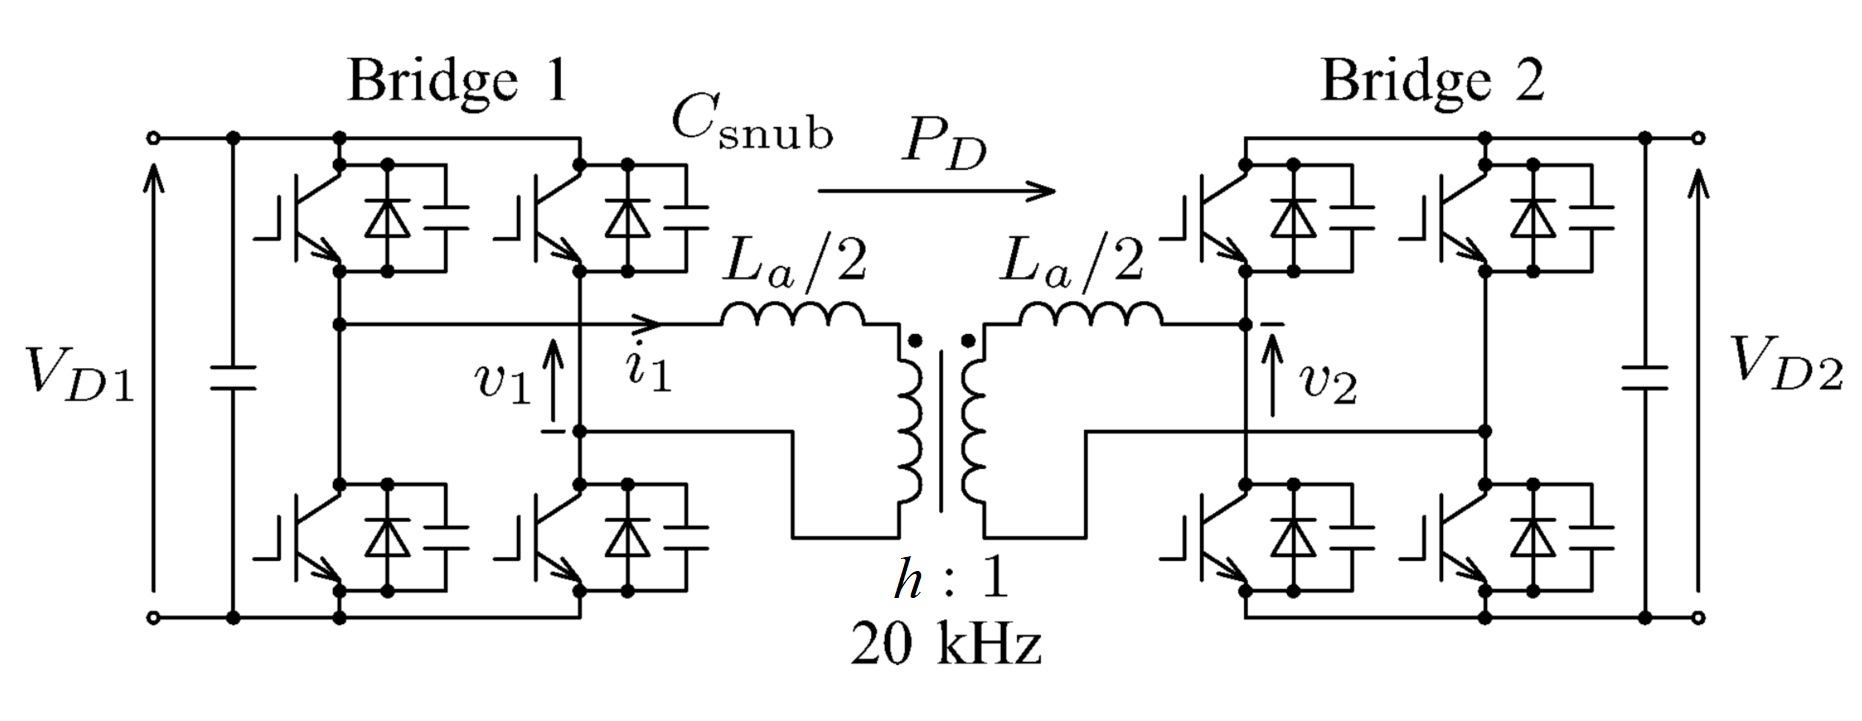
\includegraphics[width=0.7\textwidth]{EMPC_PNG_Pics/DC_DC_galvanic.png}
        \caption{Bidirectional isolated DC-DC converter, where $V_{D1}$, and $V_{D2}$ are the two end's voltage (in- and output depends on the power flow), $v_1$ and $v_2$ are the transformer voltages, $C_{snub}$ are to reduce switching loss and to damp out
over-voltage, and $h$ is the transformer turn ratio.}
        \label{BASICCSR:fig:DCDCGalvanic}
    \end{figure}
		
The principle of operation of the DC-DC converter is very simple. Two active bridges are interfaced through a transformer and are phase shifted from each other to control the amount of power flow from one DC voltage source to the other. This allows a fixed frequency, square-wave mode of operation and utilization of the leakage inductance of the transformer as the main energy transfer element. The power transfer under idealized conditions is defined as:

\begin{equation}
        \begin{array}{rcl}
            P_D&=&\frac{V_{D1}V_{D2}}{\omega L_a}\left(\delta-\frac{\delta^2}{\pi}\right)\\
        \end{array}
        \label{BASICMPC:equ:DCDC}
    \end{equation}
		
		where $\omega=2\pi f$ is the switching angular frequency of the two single phase full bridge controllers, $L_a$ is the
sum of the transformer leakage inductance.

\subsection{Current source inverters}\label{BASICCSR:sec:CSI}

Single-phase inverter's operating principles are different in each converter. The main features of the different approaches are reviewed and presented in the following. Although these converters cover the low-power range, they are widely used in power supplies or single-phase supplies. For this thesis a domestic current source inverter is considered, which fits into this category.\\
A current source inverter is composed of capacitors, switches, and diodes, where an array of two switches is called inverter leg shown in Fig.\ref{BASICCSR:fig:SingleCSI}. The capacitors required to provide a neutral point, such that each capacitor maintains a constant voltage.

\begin{figure}[!ht]
        \centering
        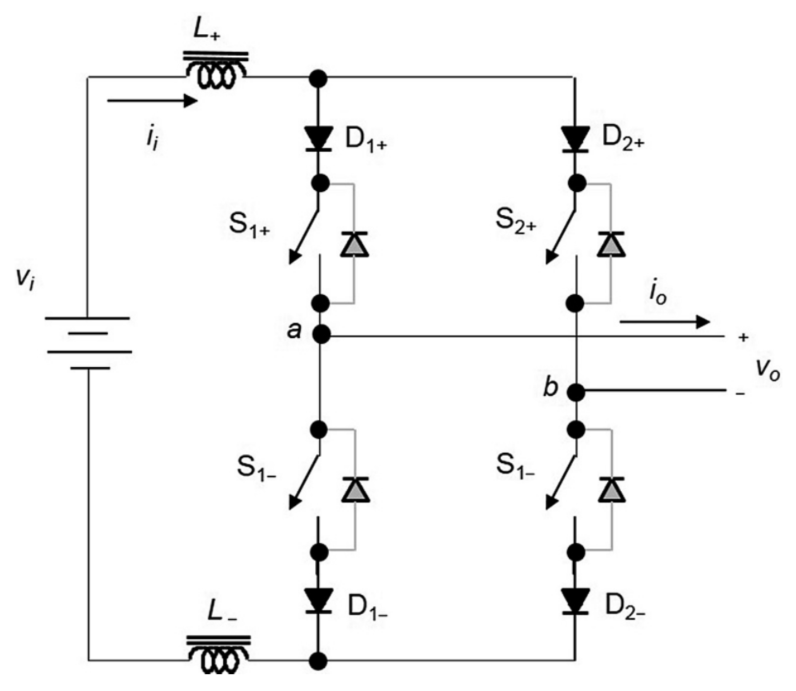
\includegraphics[width=0.6\textwidth]{EMPC_PNG_Pics/CurrentSourceInverter.png}
        \caption{Topology of a singly phase current source inverter, where $V_i$, and $V_o$ are the input and output voltages, $i_i$, and $i_o$ are the input and output currents respectively. $L_+$ and $L_-$ are current filter inductances, $S_{1+}$, $S_{2+}$, $D_{1+}$, and $D_{2+}$ are the higher switches (controlled IGBTs for instance) and diodes, and $S_{1-}$, $S_{2-}$, $D_{1-}$, and $D_{2-}$ are the lower switches and diodes respectively.}
        \label{BASICCSR:fig:SingleCSI}
    \end{figure}

The inductors required are large, such that the inductors
maintain a constant current $i_i$. Current-source topologies feature a low switching voltage gradient and reliable over-current or short-circuit protection. In order to operate properly the current-source inverter, we need to adhere to the following rules:
\begin{itemize}
\item Top or bottom switches of the different legs cannot be off simultaneously, because no current path is provided to the input inductors.
\item Diode must be placed in series with each switch, because a short circuit across the output voltage $V_o$ would be produced. If the commercial switch does not include anti- parallel diodes, then the circuit is already complete.
\item In practical implementation, an overlapping time must be considered in the control signals of the top or bottom switches of the different legs.
\end{itemize}

According to the previous rules, it should be noticed that all switches of the inverter leg can be turned on at the same time. This is not possible in voltage source inverters. There are four ($1^{st}$ to $4^{th}$) defined states of the switches and one not permitted switching state ($5^{th}$ state) as shown in Table \ref{BASICCSR:table:CSIstates}. The modulating technique should always ensure that at any instant, at least one of the top and bottom switch of the inverter legs is on, otherwise the inverter will be damaged.

% Please add the following required packages to your document preamble:
% \usepackage{multirow}
\begin{table}[h!]
\centering
\caption{Switching states of the current source inverter, where $V_{an}$, $V_{bn}$ are the $a$ and $b$ point's potential to ground.}
\begin{tabu}{|c|c|c|c|c|c|c|c|}
\hline
\multicolumn{4}{|c|}{Components conducting} & \multirow{2}{*}{State} & \multicolumn{3}{c|}{Output voltages}                \\ \cline{1-4} \cline{6-8}
$S_{1+}$       & $S_{2+}$       & $S_{1-}$      & $S_{2-}$      &                        & $V_{an}$              & $V_{bn}$              & $V_{o}$           \\ \tabucline[2pt]{-}
1         & 0         & 0        & 1        & 1                      & $V_{i}/2$            & -$V_{i}/2$           & $V_{i}$           \\ \hline
0         & 1         & 1        & 0        & 2                      & -$V_{i}/2$          & $V_{i}/2$            & -$V_{i}$          \\ \hline
1         & 1         & 0        & 0        & 3                      & $V_{i}/2$             & $V_{i}/2$            & 0             \\ \hline
0         & 0         & 1        & 1        & 4                      & -$V_{i}/2$           & -$V_{i}/2$          & 0             \\ \hline
0         & -         & 0        & -        & \multirow{2}{*}{5}     & \multicolumn{3}{c|}{\multirow{2}{*}{Not permitted}} \\ \cline{1-4}
-         & 0         & -        & 0        &                        & \multicolumn{3}{c|}{}                               \\ \hline
\end{tabu}

\label{BASICCSR:table:CSIstates}
\end{table}

The ideal waveforms are shown in Fig.\ref{BASICCSR:fig:CSIwave_All}.

\begin{figure}[h!]
                \centering
                \begin{subfigure}[b]{0.9\textwidth}
                    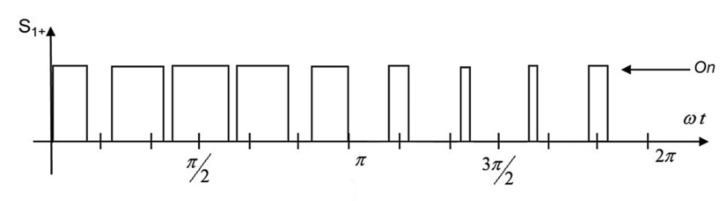
\includegraphics[width=\textwidth]{EMPC_PNG_Pics/CSIwaves_A.png}
                    \caption{\centering The state of switch $S_{1+}$.}
                    \label{BASICCSR:fig:CSIwave_A}
                \end{subfigure}
                ~ %add desired spacing between images, e. g. ~, \quad, \qquad, \hfill etc.
                  %(or a blank line to force the subfigure onto a new line)
                \begin{subfigure}[b]{0.9\textwidth}
                    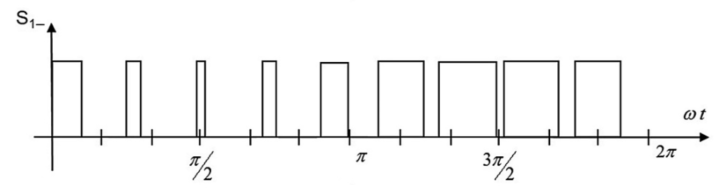
\includegraphics[width=\textwidth]{EMPC_PNG_Pics/CSIwaves_B.png}
                    \caption{\centering The state of switch $S_{2+}$..}
                    \label{BASICCSR:fig:CSIwave_B}
                \end{subfigure}
								 ~ %add desired spacing between images, e. g. ~, \quad, \qquad, \hfill etc.
                  %(or a blank line to force the subfigure onto a new line)
                \begin{subfigure}[b]{0.9\textwidth}
                    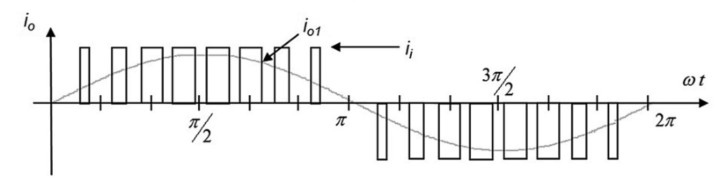
\includegraphics[width=\textwidth]{EMPC_PNG_Pics/CSIwaves_C.png}
                    \caption{\centering AC output current.}
                    \label{BASICCSR:fig:CSIwave_C}
                \end{subfigure}

                \caption{The CSI, ideal waveforms as the result of the modulation.}
                \label{BASICCSR:fig:CSIwave_All}
            \end{figure}

The states for the switches are defined by the modulating technique, which in this case is a carrier-based PWM, but unipolar output is considered. For the CSIs, different output filters may be employed, in order to provide the fundamental component of the output waveform. Depending on the application, it would be desirable to provide a voltage or current output.

\section{Asynchronous parallel pattern search}\label{BASICUNB:sec:APPS}

In the following section, the applied control structure, namely the APPS algorithm shall be discussed in detail. %Optimization (or mathematical optimization) is considered as the mathematical process of finding the best decision for a given problem within a defined set of constraints. In the simplest case, an optimization problem consists of maximizing (or minimizing) a real function by systematically choosing input values from within an allowed input set respective to the given constraints and computing the value of the function. In a controller design case, it deals with the problem of finding the optimal control law for a given system such that a certain optimality criterion is achieved with the best dynamics or lowest amount of energy required.
%The control problem includes a cost functional that is a function of state and control variables. An optimal control is a set of differential equations describing the paths of the control variables that minimize the cost function.
They commonality in this work, is that all of them are designed to search for the optimal control input for a current governing system, should it be voltage unbalance reduction with no applicable network model (due the actors unpredictability), or reaching the fastest reference value with explicit predictive control with the converter's equation's considered, which shall be discussed in section \ref{BASICCSR:sec:MPC}.\\
The APPS can rather be described as a linear search program, distributed in a multi-dimensional plane, where the it is only a black box model available \cite{kolda2003understanding}. These variants of pattern search can solve nonlinear unconstrained problems of the form of:

\begin{equation}
        \begin{array}{c}
            \min_{x\in\mathbb{R}^n}f(x),\\
        \end{array}
        \label{BASICCSR:eqn:currents}
    \end{equation}
		
		where $f:\mathbb{R}^n\longrightarrow\mathbb{R}$. We assume that the evaluation of $f$ is computationally expensive, hence our interest in using either distributed or parallel computing environments to solve the problem. It needs to be concentrated on the parallelization of the search strategy, rather than on the evaluation of $f$, though the techniques we discuss here can be adapted to handle problems for which the computation of $f$ also can be distributed. Additionally is is assumed that $f$ is continuously differentiable. It can be assumed that the gradient $\nabla f$ is unavailable, but the method is applicable as presented in section \oldref{VUB:sec:Optimization}, where the gradient determines the direction of the next step, further increasing its efficiency. For such problems, pattern search methods are one possible solution technique since they neither require nor explicitly estimate derivatives.\\

\myparagraph{Parallel pattern search}

Lets adopt an infinite sequence of iterations $\rho=0,1,2,\dots$, with the last iteration noted as $\rho-1$ and initialization at $0$. It is assumed that the process knows the best point so far as $x^{\rho-1}$, where $f(x^{\rho-1})$ is the global minima of $f$. Associated with $x^{\rho-1}$ there is a step-length control parameter namely $\Delta^{\rho-1}$. Each $i\in\mathcal{P}$, where $\mathcal{P}=\{1,\dots,p\}$ process ends iteration at $\rho-1$ by constructing it's trial point and initiating an evaluation of $f(x^{\rho-1}_i+\Delta^{\rho-1}_id_i)$, where $\mathcal{D}=\{d_1,\dots,d_p\}$ is the finite set of directions applied by each individual process. The simultaneous start of the function evaluations at the trial points on each of the $p$ processes signals the start of iteration $\rho$. When all of the participating processes are finished with their evaluation of $f$, they communicate these values to each other and determine the new values of $x^\rho$, and $\Delta^\rho$. If there exists an $i\in\mathcal{P}$, such that $f(x^{\rho-1}_i+\Delta^{\rho-1}_id_i)<f(x^{\rho-1})$, then $\rho\in\mathcal{S}$, where $\mathcal{S}$ denotes the successful iterations.

\myparagraph{Adding asynchronicity}

 With said above, the general strategy for asynchronous parallel pattern search, from the perspective of a single process $i\in\mathcal{P}$ can be outlined:
		\begin{enumerate}
		\item Evaluate $f(x^{best}_i+\Delta^{best}_id_i)$.
		\item If $f(x^{best}_i+\Delta^{best}_id_i) <f(x^{best}_i)$, then broadcast result to all other processes.
		\item Update local values $x^{best}_i$ and $\Delta^{best}_i$ based on the current local information.
		\item Repeat.
		\end{enumerate}
	The price payed is that each process has its own notion of the best known point seen so far, as well as its own value for	$\Delta^i$. Any success on one process is communicated to all other processes participating in the search, but the successful process carries on from its new best point without waiting for a response from the other processes. By adding a few mild conditions, the global convergence of the search can be still ensured \cite{kolda2003understanding}.  Instead of indexing based on a notion of iterations, we switch from $\rho$ to indexing based on discrete time instance, letting the set $\mathcal{Q}=\{1,2,\dots,q\}$ denote the index of steps. Thus $x_i^q$ s used for the best point known to process $i$ at time step $q$, and similarly, $\Delta_i^q$.  So if process $i$ starts a function evaluation at time step $q$, the trial point at which the function evaluation will be made at $x^{q}_i+\Delta^{q}_id_i$. Further worth mention, that time steps are assumed to be of fine enough resolution so that at most one function evaluation finishes per process per time step.\\
	Lets define two sets that satisfy $\mathcal{Q}=\mathcal{S}_i\cup\mathcal{U}_i$, , and $\mathcal{S}_i=\mathcal{I}_i\cup\mathcal{E}_i$, where $\mathcal{S}_i$ is the set of all time successful steps on process $i$, $\mathcal{I}_i$ is the set if internal successes, $\mathcal{E}_i$ is the set of external successes,   and $\mathcal{U}_i$ consists the unsuccessful steps respectfully. An internal success, where the process finds itself the minima, the external success is where the process is updated externally by the minima. Further  $\mathcal{C}_i\in\mathcal{U}_i$ is defined as the set of time steps where $\Delta^t_i$ is reduced. All the above cases ($\mathcal{U}_i\textbackslash\mathcal{C}_i$) no action is performed.\\
	The updating functions allow us to give the following general definitions for $x_i^q$ and $\Delta^q_i$. For every $q\in\mathcal{Q}$, $q>0$, the best point for the $i^{th}$ process defined to be:
	
	\begin{equation}
        \begin{array}{rcl}
            x_i^q&=&\begin{Bmatrix}
                x_{\omega_i(q)}^{\tau_i(q)}+\Delta_{\omega_i(q)}^{\tau_i(q)}d_{\omega_i(q)},&\textnormal{if }q\in\mathcal{S}_i\\
                x_i^{q-1},&\textnormal{otherwise}\\
            \end{Bmatrix},\\
        \end{array}
        \label{BSIC:equ:APPS_x}
    \end{equation}
		
		with the initialisation $x^0_i=x^0$, where $\omega_i(q)$ is the generating process index for the update time at step $q$ on process $i$, and $\tau_i(q)$ is the time index for initialization of the function evaluation, that produced the update at time $q$ on process $i$. For every $q$ the step length control parameter $\Delta_i^q$ defined to be:
		
		\begin{equation}
        \begin{array}{rcl}
            \Delta_i^q&=&\begin{Bmatrix}
                \lambda_{\omega_i(q)}^{\nu_i(q)}\Delta_{\omega_i(q)}^{\tau_i(q)},&\textnormal{if }q\in\mathcal{S}_i\\
								\theta_{i}^{q}\Delta_{\omega_i(q)}^{\tau_i(q)},&\textnormal{if }q\in\mathcal{C}_i\\
                \Delta_i^{q-1},&\textnormal{otherwise}\\
            \end{Bmatrix},\\
        \end{array}
        \label{BSIC:equ:APPS_Delta}
    \end{equation}
		
		with the initialization $\Delta^0_i=\Delta^0$, where $\nu_i(q)$ is  time index for the completion of the function evaluation that produced the update at time step $q$ on process $i$, and $\theta_i^q$ and $\lambda_i^q$ are chosen. With the following pattern followed, the \hlc[MA]{local} minima of $f$ shall eventually reached \hlc[MA]{with} undetermined steps. 
\section[Unbalance compensation with asym. inverter]{Voltage unbalance compensation with optimization based control algorithm and asymmetrical inverter structure}\label{VUB:sec:Compensation}

\hlc[PT]{This chapter describes the compensation of voltage unbalance (VU) of an unknown low voltage domestic network, with a current source power electric device, utilizing a PV power source and a lithium battery. The goal is, to reduce the VU on the network utilizing the limited resources, what the PV unit and the stored energy has to offer. With this in mind, the device is connected to any three phase four wire 400V connection point, and based on only on the measured network voltage, shall formulate such constrained harmonic current waveforms, that results in unbalance reduction based on the prescribed const function ($VUF$, or $G$, described in} \oldref{VUB:sec:Geom})\hlc[PT]{. Keep in mind, that the network transformer station's current and other properties, as well as the number and nature of the connected household size loads, and the network topology is unknown for the device. Furthermore, the loads connection and disconnection patterns (as such the network impedance) are time variant, with unknown stochastic distribution function.}\\
\hlc[PT]{Throughout the chapter, first the control problem shall be analyzed in detail, and the constraints and scope the formulation is operated with. Next the power electronic device's topology, and capabilities shall described, with a possible use case measured on a real connection point at the campus laboratory. Next in section} \oldref{VUB:sec:Optimization} \hlc[PT]{is the description of the optimization based algorithm's is written, and the argumentation why the particular method was used, and why is it suitable for the control problem previously outlined. The chapter closes with the simulation results performed in Matlab/Simulink and the discussion on the performance results, and the comparison of the device's operation modes.}
    %%
 %First the networks structure shall be described, the power electrical device is connected to, as a household supplying, renewable utilizing device, followed by the aforementioned device's topology and control shall be presented based on the geometrical voltage unbalance norm (described in section \ref{VUB:sec:Geom}), with the performance results on an unbalanced network. It shall be shown, that it is possible to formulate some power quality related aims, or demands for the domestic size generator units implemented in a complex power electrical system, capable of supplying a household, with both renewable and network supplied energy, and lowering voltage unbalance as well, considering a network with unpredictable impedance.

\subsection{Problem statement}\label{VUB:sec:Statement}

    The network, the proposed VU compensator supposed to be connect, is a three phase four wire low voltage domestic transformer area. depicted in Figure \ref{fig:network}. As such, the overwhelming loads, are assumed as single phase, with resistive (e.g.: heaters) inductive (e.g.: motors) and capacitive (e.g.: chargers) properties as well, while some of them are symmetric three phase ones (e.g.: induction ovens, compressors, inverter fed motors).

    \begin{figure}[!ht]
    \centering
    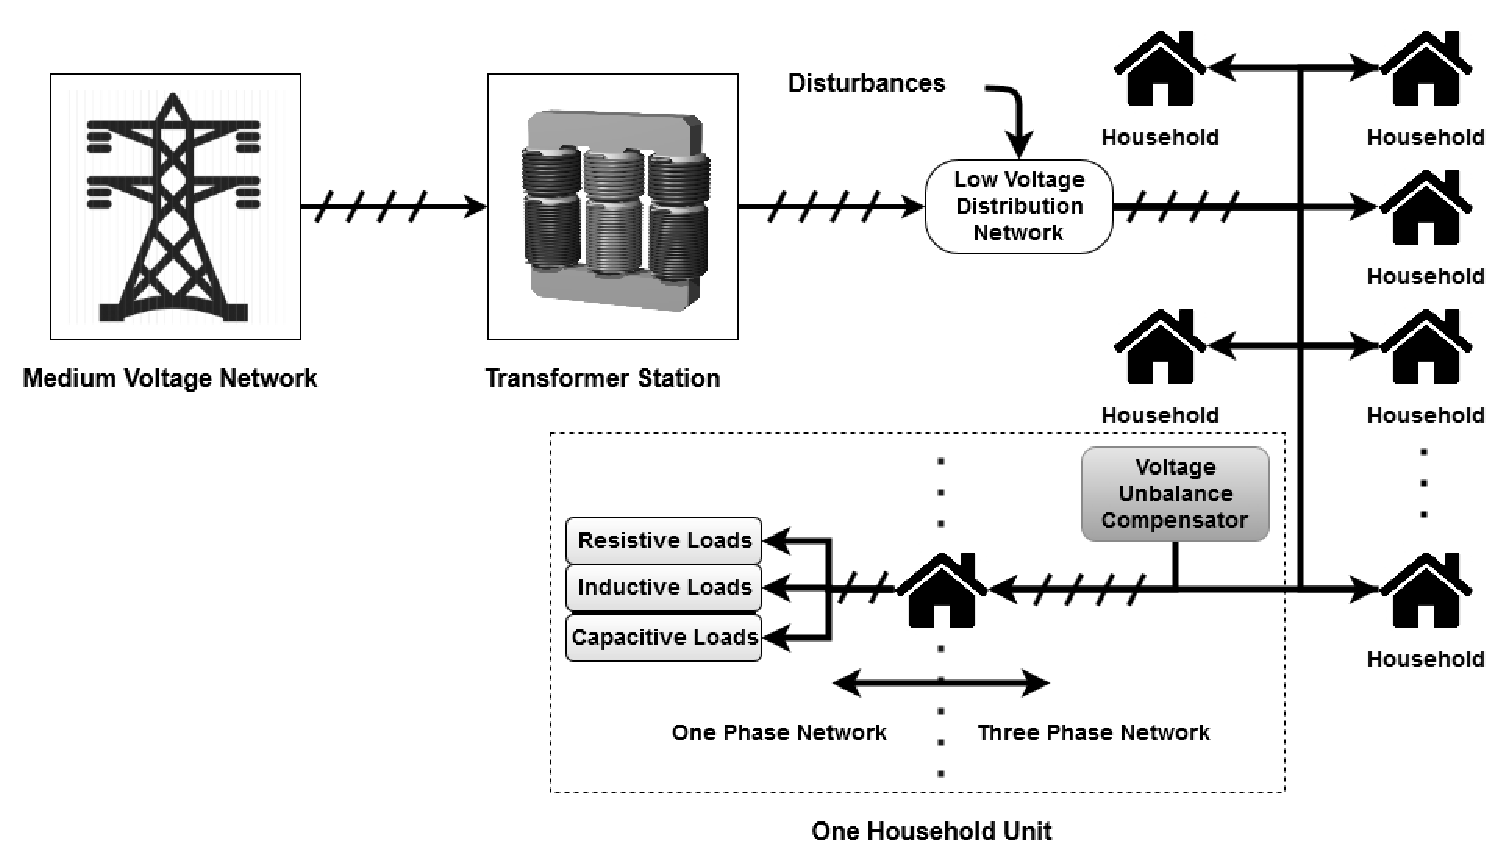
\includegraphics[width=\textwidth]{Unblance_EPS_Pics/network_gray.eps}
    \caption{The simplified structure of a three phase four wire low voltage network. Several regular households are representing the main loads, and connected with power line sections, subject to inductive and resistive disturbances and capacitive couplings. Domestic powerplants may connect to any connection point within the low voltage section, via an appropriate inverter - either to the three phase sections using a three phase inverter or to a single phase using a single phase inverter.}
    \label{fig:network}
    \end{figure}

    Due to the unregulated, and uneven load, or (with the emergence of affordable PV stations) possible domestic powerplant distribution, the voltage and current unbalance present in the network causes additional power loss inside the medium voltage/low voltage transformer and in the transportation line wires too. It also has undesired effects in certain three phase loads, mainly rotating machines where it causes torque reduction and pulsating torque effect. Large scale unbalance can also activate automatic protection functions of electricity dispatch system causes power outage. These negative effects lower the electric power quality and rises the cost of electrical energy and rises the carbon footprint of our everyday life, and also undesirable for the customers and adds maintenance cost to the service provider.\\
    \hlc[PT]{This chapter's aim to propose a model and control scheme for a three phase instrumentation, which can compensate voltage based unbalance, and as such lower the power losses and increase power quality, not only at the domestic connection point but in the whole low voltage transformer area without prior knowledge of the network's topology, it's connected load's, or the transformer characteristics. Also doing so with the energy provided by a PV source and stored energy in a battery bank, or in some cases, via 'zero balance operation' where the power reserves are empty.}\\
    As such, the measured voltage of the network serves as indicator of VU and the cost function can be formulated as \ref{eqn:VU_costfcn}:

    \begin{equation}
    \label{eqn:VU_costfcn}
    \begin{array}{rcl}
    J_{VUF}(V_{abc},i_{abc})&=&\min_{i_{abc}}f_{grid}(g_{VUF}(V_{abc}),i_{abc}),\\
    \textnormal{or,}&&\\
    J_{G}(V_{abc},i_{abc})&=&\min_{i_{abc}}f_{grid}(g_{G}(V_{abc}),i_{abc}),\\
    \end{array}
    \end{equation}
    \textcolor{red}{ATTILA KÉRLEK EZT ELLENŐRIZD!}\\
    where, $J_{VUF}$ and $J_G$ are the state of the art ($VUF$) and proposed geometrical ($G$) cost functions, $f_{grid}$ is the network's function, $g_{VUF}$ is described by \ref{BASICUNB:equ:symmetry}, $g_{G}$ is described by \ref{equ:geom}, $V_{abc}$ is the measured voltage from the network, and $i_{abc}$ is the current injected or consumed by the device.\\

    %\subsection{Control problem}\label{VUB:sec:Control}

    The above problem statement specifies the scope solution space together with the solution method. \hlc[PT]{It can be observed in Fig. }\ref{fig:mininetwork}\hlc[PT]{, that the system of interest is the power grid with all the unknown stochastic and nonlinear phenomena, represented as a black box model, with limited observability through the measured voltage ($V_{abc}$). It is worth mentioning, that current measurement is only available at the poles and inside the device, since after the household meter or at the transformer poles, current measurement would be expensive, although the global network VU is observable at this connection point also. The input to the system are current signals (one current in the single phase case and three in the three phase setup), which are naturally constrained by the available energy of the household, stored in a battery pack or momentarily generated by the wind or solar generator unit. The response of the system can be either the current or the voltage measured at the connection point of the inverter unit, however, the general legal regulations only allow voltage measurement for consumers.}\\

     %\begin{figure}[!ht]
%    \centering
%    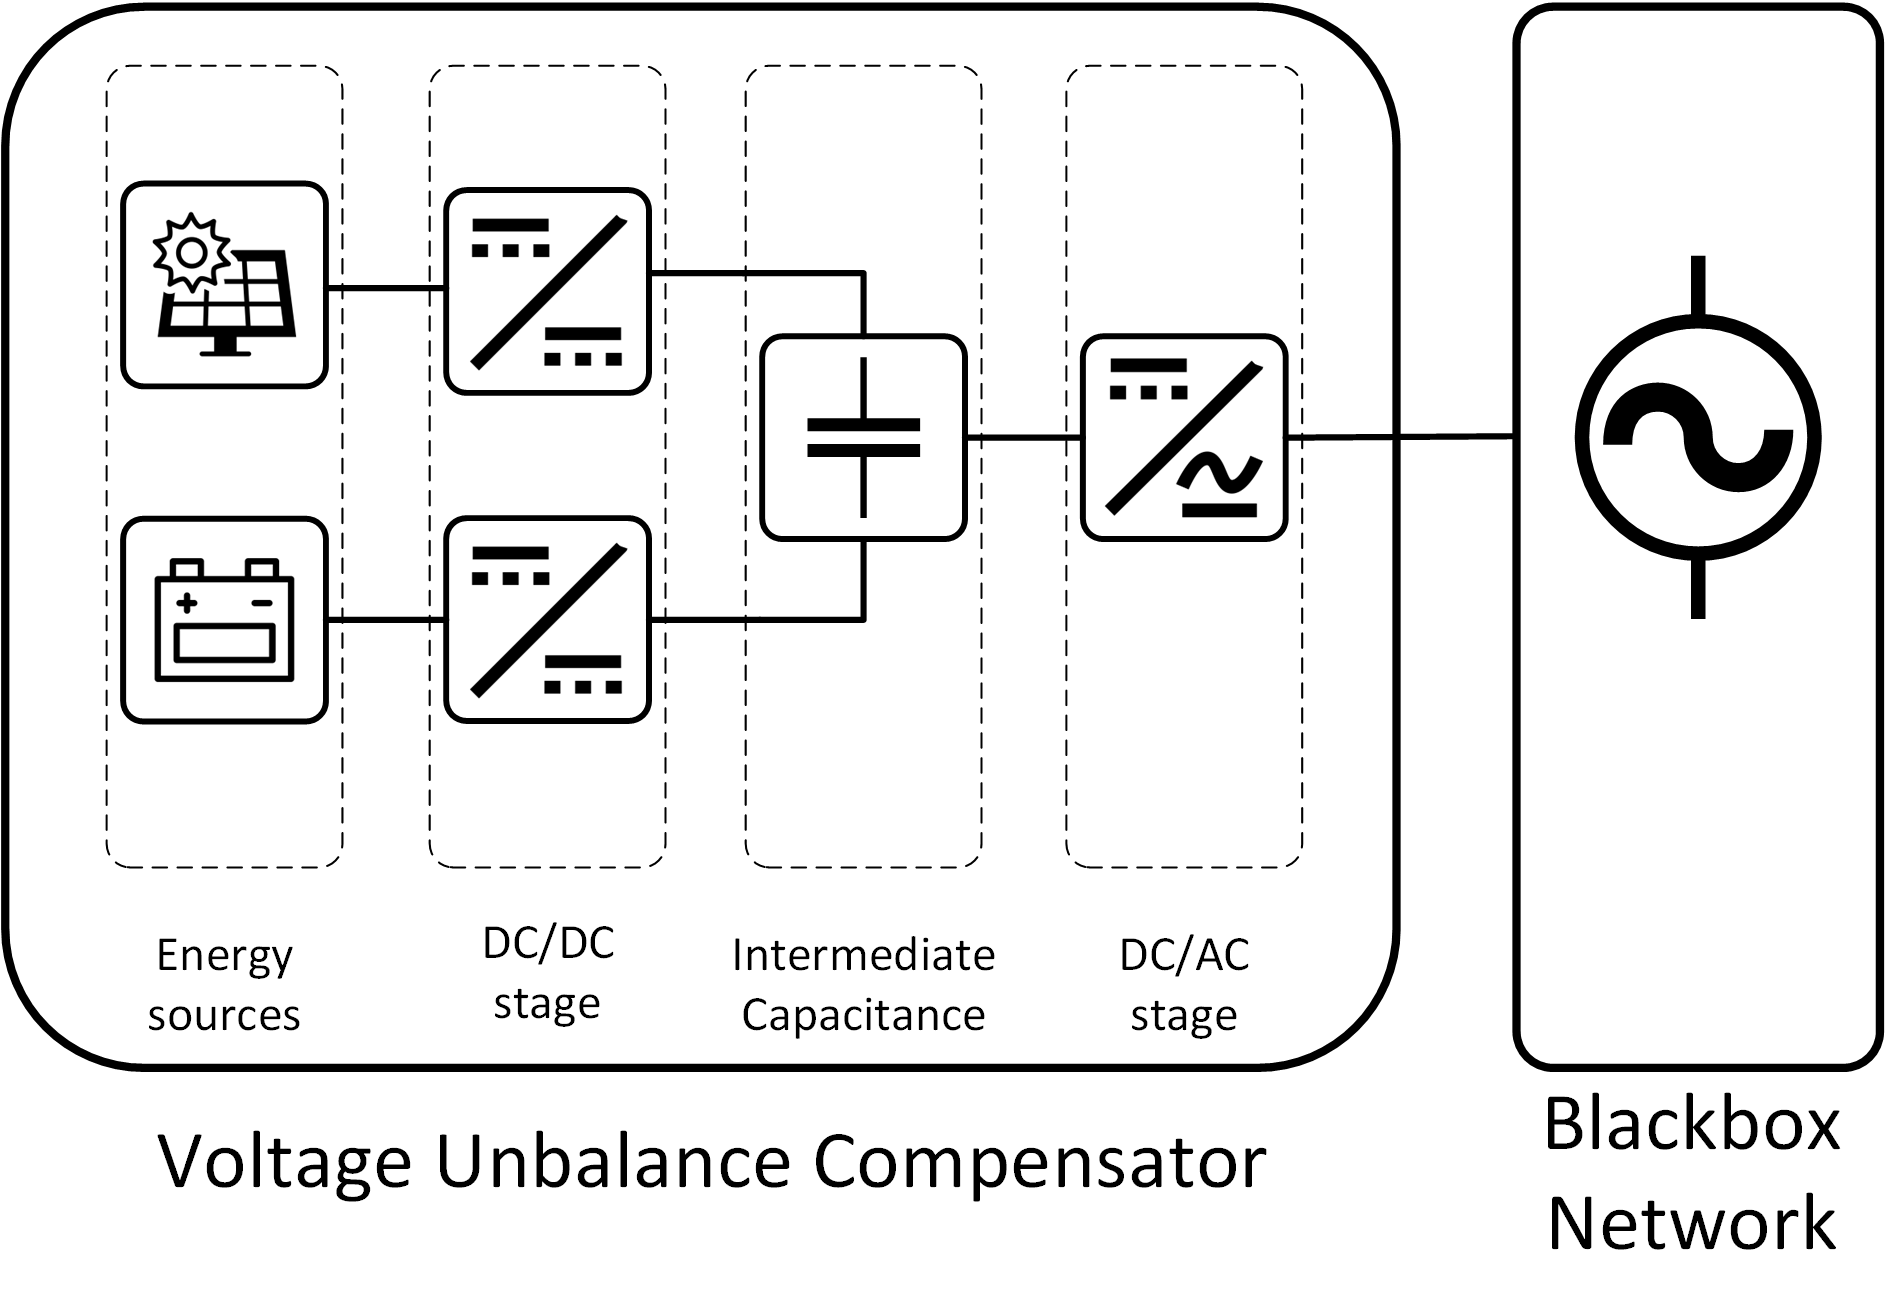
\includegraphics[width=.6\textwidth]{Unblance_EPS_Pics/VUCompensator_minichart.png}
%    \caption{Simplified compensator perspective and overview.}
%    \label{fig:mininetwork}
%    \end{figure}

    \begin{figure*}[ht]
        \centering
        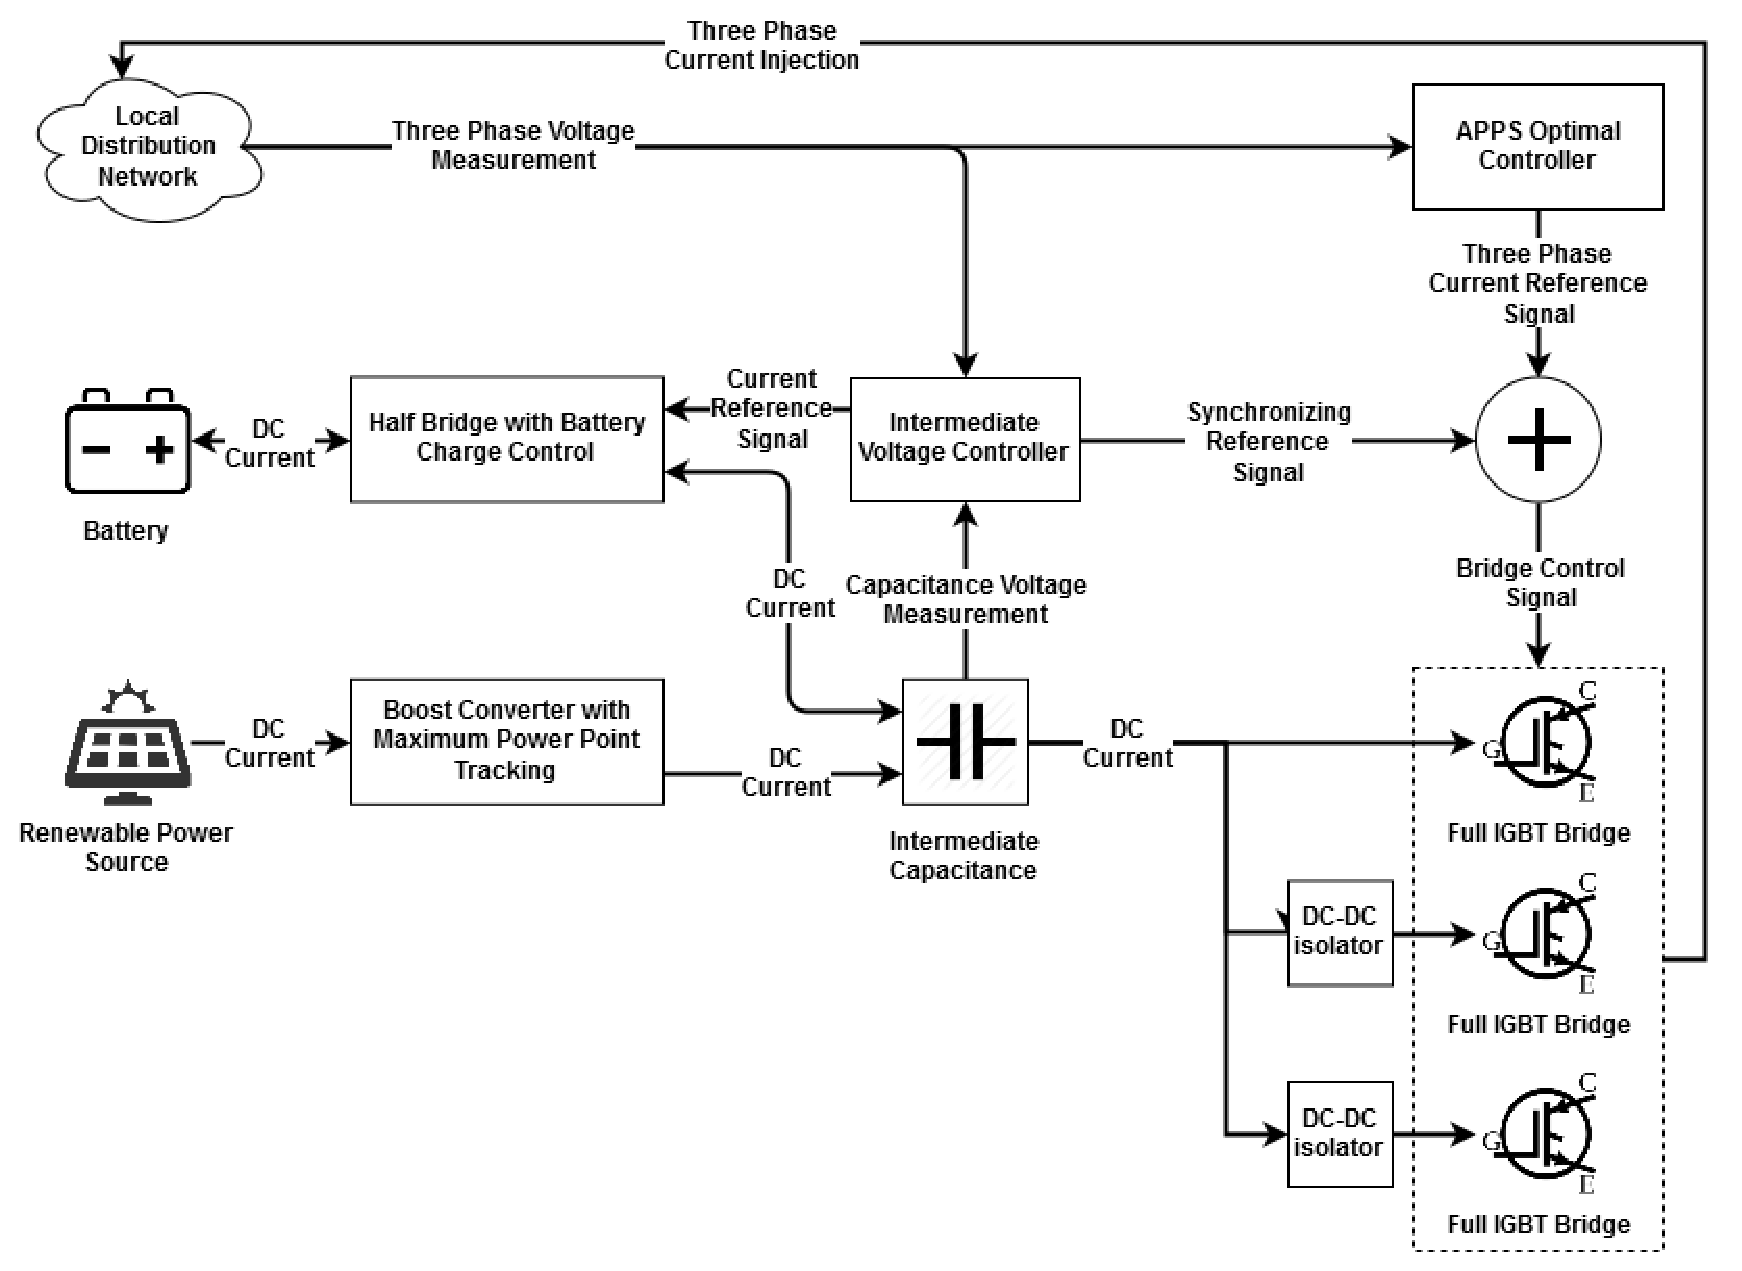
\includegraphics[width=0.95\textwidth]{Unblance_EPS_Pics/inverter.eps}
        \caption{The asymmetrical inverter design, which applies three single phase full bridge IGBT current injector to create the injected asymmetrical current shapes for voltage unbalance compensation.}
        \label{fig:inv}
        \end{figure*}


    The difficulty of the control problem comes from the fact, that there are no mathematically tractable models of the network can be generated because of its unpredictable and nonlinear features. This means, that in these conditions only black-box methods can be applied for this system.
    For the control aim it is a natural choice to minimize the actual voltage unbalance of the low voltage local transformer area measured (or calculated) at the connection point of the inverter. Several optimization based methods are available for such kind of optimal control problems, e.g. \cite{gorbe2012reduction} where the only bottleneck is the computational efficiency since the implemented controller has to run on the commercial inverter's hardware (digital signal processor unit).

    \subsection{Optimization based control algorithm}\label{VUB:sec:Optimization}

        Ideally, the point $\textbf{x}^q$ corresponding to the local minimum, which can be calculated from the negative gradient $\nabla f(\textbf{x})$, that gives the value and direction of the corresponding step in the parameter space, as such making the optimization straightforward. The next step is made in the direction of gradient with the proper sign. Most of the time, this sequence of steps, converges to local multivariate extreme value $\textbf{x}^q$ of the function \ref{eqn:contstruct1}.

        \begin{equation}
        \begin{array}{rcl}
        \label{eqn:contstruct1}
         \textbf{x}^{(q)}&=&\textbf{x}^{(q-1)}-t_q\nabla f(\textbf{x}^{(q-1)}),\\
         %q&\in&\mathbb{N},\\
         \end{array}
        \end{equation}

        where $q\in\mathbb{N}$, and $t_q$ resembles the step time of the algorithm.%
        Unfortunately, the controlled electrical system is described by multivariate non-linear differential equations, the optimization of which is infeasible to derive using the differentiation of an error function. Therefore, the optimization methods based on direct differentiation are not applicable. In such cases, when high computational power is needed for performing long time-consuming simulations, the so called asynchronous paralell pattern search or APPS method can utilized.\\
        \hlc[PT]{There is a long history for identifying VU on the network as presented in section}\oldref{BASICUNB:sec:DefinitionsofUNB}\hlc[PT]{ As such the basis of the const function is well defined in} \ref{eqn:VU_costfcn}. \hlc[PT]{Since the network is assumed not only non linear and  time variant, with unknown stochastic distribution function, the mathematical representation of the network from the device's perspective would be a difficult task. As such the network's voltage response to a certain current injection is hard to predict, and could make the situation even worse, distorting the voltage phasor even further. Wit this in mind regular PID controllers are not sufficient, although there were attempts to solve similar control problems with artificial intelligence} \cite{el2011active}.\\
        For this purpose I choose an asynchronous parallel pattern search method (APPS) to control our scenario \cite{hough2001asynchronous}, \cite{kolda2003understanding}. The methodology and formulation of the APPS method is described in more detail in section \oldref{BASICUNB:sec:APPS}.

        It can be assumed, that the network function $f_{grid}$ from \ref{eqn:VU_costfcn} is hard to estimate, as such, the best approach is to use parallel computing environment to solve the problem, instead of function evaluation. Since $f_{grid}$ is continuously differentiable, it can be further assumed, that it's gradient $\nabla f_{grid}$ unavailable and also unreliable to approximate to the non linear time variant network operation. For this type of problems, so called pattern search methods are one possible solution, since they neither require nor explicitly estimate derivatives.  Pattern search methods also have a long history of success when applied to non linear problems \cite{hough2001asynchronous}.\\
        With this in mind the list of processes which could be parallelized, comes from shape of the voltage phasor itself (observed in Fig. \ref{fig:threephase}). The ideal phasor is deviating in terms of voltage amplitudes and angles. As such, if the first phase $V_a$ is is locked by angle, it can be assumed, that the ideal phasor can deviate by two phases and three amplitudes. As such the search algorythm has five processes (or axes) to optimize along. Basically the general strategy for the APPS method, from a single process perspective follows: \textcolor{red}{Attila, az algoritmust nézd át kérlek hogy konzisztens-e!}

        \begin{algorithm}[H]
        \SetAlgoLined
        %\KwResult{Write here the result }
         $\textbf{x}_i^0=0$, $\Delta_i^0=0, d_i^{(q)}=1$\;
         %\While{$f_{grid}(\textbf{x}_i^{q}+\Delta_i^{(q)}d_i^{(q)})\neq0$}{
         \While{$f_{grid}(\Delta_i^{(q)}\neq0$}{
          $N^{(q)}=f_{grid}(\textbf{x}_i^{(q)}+\Delta_i^{(q)}d_i^{(q)})$\;
          $d_i^{(q)}=0.5(sign(N^{(q-3)}-N^{(q-2)}+sign(N^{(q-4)}-N^{(q-3)})))$\;
          $\Delta_i^{(q)}=n_{i}N^{(q-1)}\Delta_i^{(q-1)}+\Delta_i^{(q-2)}+m_{i}N^{(q-1)}$\;
          \eIf{$f_{grid}(\textbf{x}_i^{(q)}+\Delta_i^{(q)}d_i^{(q)})<f_{grid}(\textbf{x}_i^{(q)})$}{
          $\textbf{x}_i^{(q+1)}=\textbf{x}_i^{(q)}+\Delta_i^{(q)}d_i^{(q)}$\;
          $I_{APPS}=f_{current}(\textbf{x})$\;
          $I_{abc}=\frac{V_{abc}}{R_{virt}}f_{Inter}(V_{inter})+I_{APPS}$\;
           %<bradcast new result of $f_{grid}$ to other processes>\;
           }{
          }
          }
         \caption{APPS for VU reducing optimal current calculation}
         \label{algo:APPS}
        \end{algorithm}
        where $f_{grid}$ representing the multi variate voltage response function of the grid of which cost ($VUF$ or $G$)
        function could be calculated, based on current injection, $f_{current}$ updates and formulated the three phase current waveform based on the amplitude and voltage values $\textbf{x}$ vector represents, and $f_{inter}$ represents the intermediate buffer capacitance's PID voltage controller. The function arguments are $\textbf{x}_i$, the actuator for the $i^{th}$ process aka. the amplitude or phase of the three phase current phasor, needs to be applied on the system, for VU reduction. This value is later offsetted by the normalised value of internal capacitance, $V_{Inter}$, and the scaled value of the network voltage $V_{abc}$ by a virtual resistance $R_{virt}$. Since the injected currents are synchronised via initial Fast Fourier Transformation (FFT), this operation could be performed. Furthermore, $\Delta_i$ the process step length aka. the value of the current vector's amplitude or angle needs to be changed for a successful step, and $d_i$ is the corresponding step's signed direction vector, which specifies the applied changes direction. Furthermore $N$ represents the chosen nor's value as the network's response to the current injection, and $n_i$, and $m_i$ are scaler gains for the corresponding process. The algorithm is initialised with $\textbf{x}_i^0=0$, $\Delta_i^0=0$ for a smooth start, due to lack of prior network knowledge.

        \begin{figure*}[h]
        \centering
        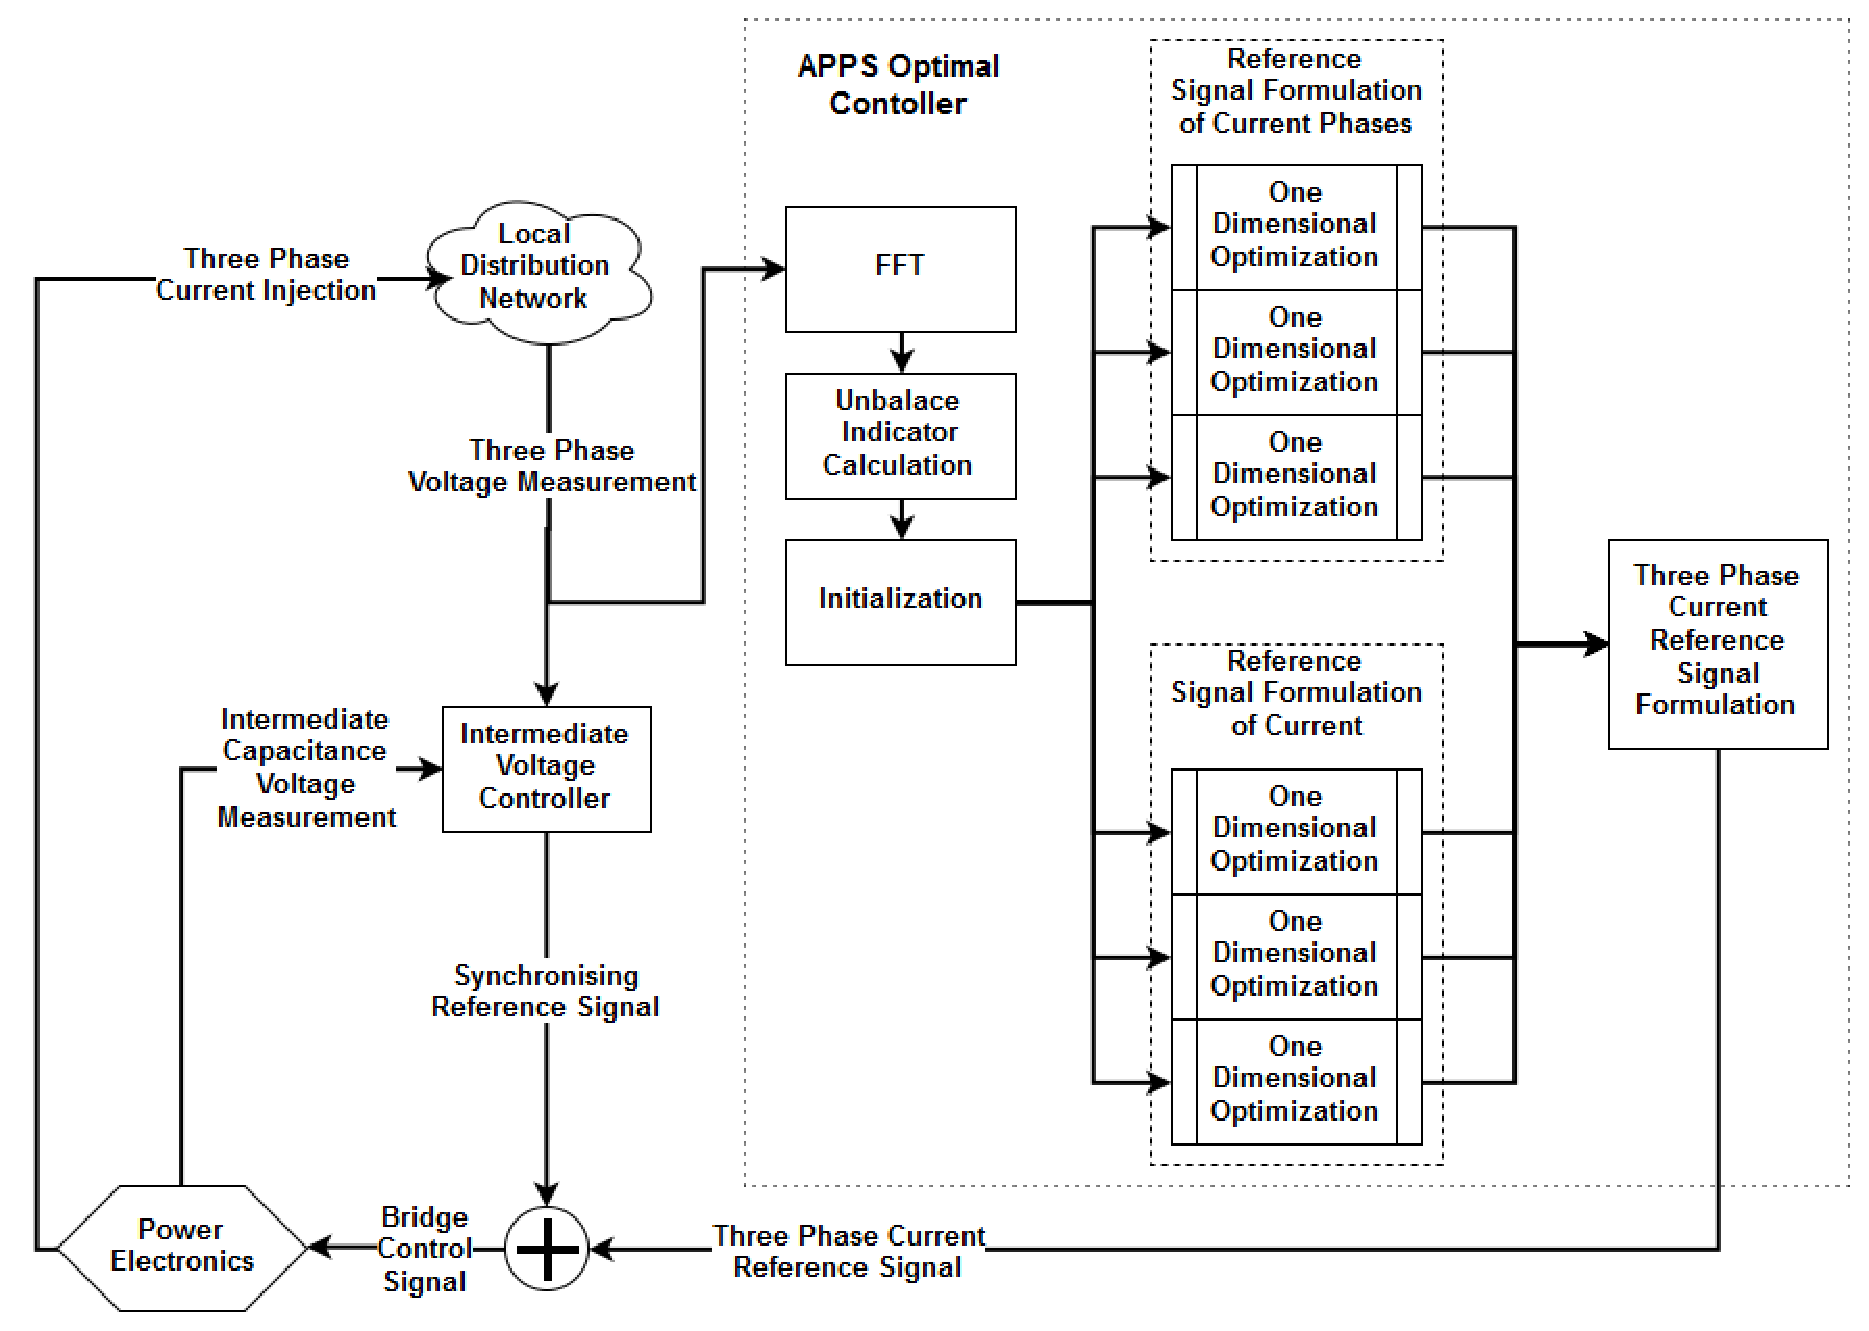
\includegraphics[width=0.95\textwidth]{Unblance_EPS_Pics/APPS_1_2_.eps}
        \caption{The optimization algorithm implemented for current control. A one dimensional linear optimization step is being solved in each dimension of the six dimensional parameter space, iteratively.}
        \label{fig:APPS}
        \end{figure*}

        %\textbf{red}{régi részek:}\\
         The search pattern $p$ is based on the sampling of the error function (selected norm) on $f_{grid}$, and it corresponds to variables or subsets of variables in each point in the independent variable or parameter space. At the same time, the norm values at these points can be calculated independently if $\Delta_q>0$, using algorithm \ref{algo:APPS}.
				
        %\begin{equation}
%        \label{eqn:contstruct2}
%        \begin{array}{rcl}
%         \textbf{x}^{(q+1)}&=&\textbf{x}^{(q)}+\Delta_qd_i \\
%         \mathrm{if}&&f(\textbf{x}^{(k)}+\Delta_qd_i) \leq f(\textbf{x}^{(q)}),\\
%         %q&\in&\mathbb{N}\\
%         \end{array}
%        \end{equation}

        The parameter is $\textbf{x}^q\in\mathbb{R}^n$, and the \hlc[PT]{initial} search pattern $\textbf{p}\in\mathcal{D}={d_1,...d_n}$ is taken from a predefined finite set\hlc[PT]{, and updated every iteration}. In this case, the error function \hlc[PT]{result} of $N$ should be calculated for each pattern $\textbf{p}$. As the competing directions are different, \hlc[PT]{as} there is \hlc[PT]{too much complexity} for direction vector $\textbf{p}$ \hlc[PT]{to be jointly calculated, as with model based optimizers}, synchronization should not be maintained. This is the asynchronous case, where an individual $\textbf{p}$ vector is defined for each output variable, and the optimization was performed in each direction asynchronously and shifted in time. Most likely, the error function has a single local minimum as a symmetric amplitude and phase values. Approaching the minimal value of norm, the controller uses adaptive increments that are proportional to the norm itself. Because of the complex interactions between the components of the controller, \hlc[PT]{an the unknown network impedance} only one parameter is changed at a time, even if the values of the amplitude and phase components in specific time slot changes. The algorithm moves along the six axes of six separate time slots close to the local minimum $N$.\\
        Unlike other similar approaches, e.g. \cite{segui2007approach}, the explained optimal controller does not rely on a measured current signal (which varies according where the measurement took place on the grid and renders the global optimization unreliable) but rather measuring and analyzing the voltage unbalance via the proposed indicator and optimizes the voltage shape, the latter of which depends on the nonlinear distortion of the whole low-voltage transformer area and determines additional power losses. The controller's performance was compared to a non compensated network, and a network consisting synchronized symmetric power intake from a regular inverter.\\
        In each iteration only one physical value is changing on the six dimensional parameter field, which consists of the three amplitude and three phase values. If the change effects with cost function reduction (the reference norm's normalized value), the controller holds the new value of amplitude or phase for the controlled current sources (Figure \ref{fig:APPS}). The advantage of this controller structure that is not necessary to know the controlled value's behavior well, like we could not determine the number and type of the other loads on the network \cite{Neukirchner2015}. There are however two disadvantages. First is the low speed of control, due to the several necessary iterations (depending on the circumstances) to find the optimal directions in the parameter space, and the serial nature of interventions and norm calculations. The second comes from the method itself since the controller may stuck in local minima.

    \subsection{Asymmetrical inverter structure}\label{VUB:sec:Inverter}

    \hlc[PT]{For the purpose of VU compensation, the} energy injection is realized increasingly, and applied directly to the three phase low voltage grid with only a domestic size PV power plant as source of power \hlc[PT]{and the energy stored in an attached battery if possible.} More and more manufacturers produce three phase grid synchronized inverters from 5\,kW size. These equipments implement accurate symmetrical current feed with a standard three phase full bridge structure, consists of six Isolated Gate Bipolar Transistors (IGBT). The demand is to employ a current source single phase structure with aforementioned controllable switches in section \oldref{BASICCSR:sec:CSI}. This is a standard structure suitable for symmetric harmonic current injection. It has limited capacities to inject not totally symmetric 3 phase current time functions, but Kirchhoff's current law permits only constant zero-sum current time functions injected with this structure. There are examples with this type of asymmetric current injections in the literature \cite{lee2009new}.\\
    \hlc[PT]{The compensation requires a three phase current waveform, in accordance to the requirements to reduce VU on the network, and since the voltage phasor is distorted, the compensation current phasor is assumed to distorted as well. This means only the frequency is given but each phase shall have different characteristics, independently, as the APPS dictates. This is by default not achievable by regular three phase current source inverter (CSI) topologies, since, to try to produce such distorted waveforms would cause malfunction, as it was uncovered from the literature in section} \oldref{BASICCSR:sec:literature}.
    \hlc[PT]{As such an asymmetrical inverter structure is required, where} zero line connection is needed for the differential current. In this setup, 3 different full bridge single phase current inverters are used to supply each phase of low voltage transportation lines, \hlc[PT]{similarly, like the authors of} \cite{Patnaik2013topologies}. This way it is most sufficient to use bi-directional power flow, with galvanic decoupling, but with a current controlled fashion (shown in section \oldref{BASICCSR:sec:CSI}). This isolation can be reached  with using isolation transformers in the supply side, although it is preferable to use as a complex energetic system with specific inside DC bus system fed from \hlc[PT]{PV panel} or batteries. \hlc[PT]{This way,} at least 2 full bridges with two way DC-DC converters (described in section \oldref{BASICCSR:sec:DCDC}) are required. This can complicate the physical realization but easy to simulate with two controlled power source. Other possible easy to realize solution to isolate the full bridge outputs  connected to three phase lines with isolating transformers. It is recommended due to electric shock protection reasons.\\
    This design method doesn't allow to produce DC current components \hlc[PT]{and it is not component and cost optimized, as such it is recommended to re-iterate to a better solution in the future}. \hlc[PT]{The main} drawback of this solution is the complex difficult control method of the half bridges, to keep the current sum in zero values in each moment, and to provide the correct current paths inside the inverter. This structure has the lowest production cost, but in the phase of proofing the asymmetry compensation we chose the DC-DC isolated  full bridge design for simulation purpose because of the simple control during simulation. Possible elegant solution to supplement the standard three phase inverter design with a fourth half bridge for Zero line, building a specific four leg inverter design \cite{Ninad2014control}.\\
    The injection of \hlc[PT]{non-harmonic} current shapes will be \hlc[PT]{also} necessary in order to decrease the extant THD of the network, \hlc[PT]{but this is currently out of the dissertation's scope}.\\
    These expectations yield an inverter with new structure suitable for arbitrary current injections without limitations. The design lends similar elements like in \cite{gorbe2012reduction} by means of battery charge, renewable power point tracking, intermediate voltage, and IGBT bridge control, but in this case the problem requires a three phase solution for the voltage unbalance reduction.\\

    \subsubsection{Topology}\label{VUB:sec:topology}
    The applied structure based on a full bridge IGBT structure used in single phase current injection. Three different IGBT full bridge were connected at the output point, thus our structure has three phase and neutral connection too, to carry out any current form. The disadvantage of this structure is that it needs 12 IGBTs in the output stage as opposed to the 6 IGBTs needed for a classical full bridge structure and needs three galvanically isolated direct current (DC) voltage source for feeding.\\
    The other standard elements, that the inverter design consists:

        \begin{itemize}
            \item Standard maximum power point tracking (MPPT) input stage, to inject the maximum available power from the renewable source to the intermediate voltage capacitor with a simple controlled boost converter
            \item A half bridge current controller to charge or deploy the battery pack connected to the complex energetic system for energy storage and energy unbalance compensation
            \item Intermediate voltage controller
            \item Universal three phase output stage with 3 single phase full bridge IGBT current injector and 2 high current DC-DC converter
        \end{itemize}
    This is suitable to inject any necessary current shape to the low voltage three phase grid even DC currents too. Later a power loss and production cost analysis will be necessary if the built structure will be suitable for asymmetric compensation of low voltage transformer area.
    %\pagebreak

        \begin{figure}[h]
        \centering
        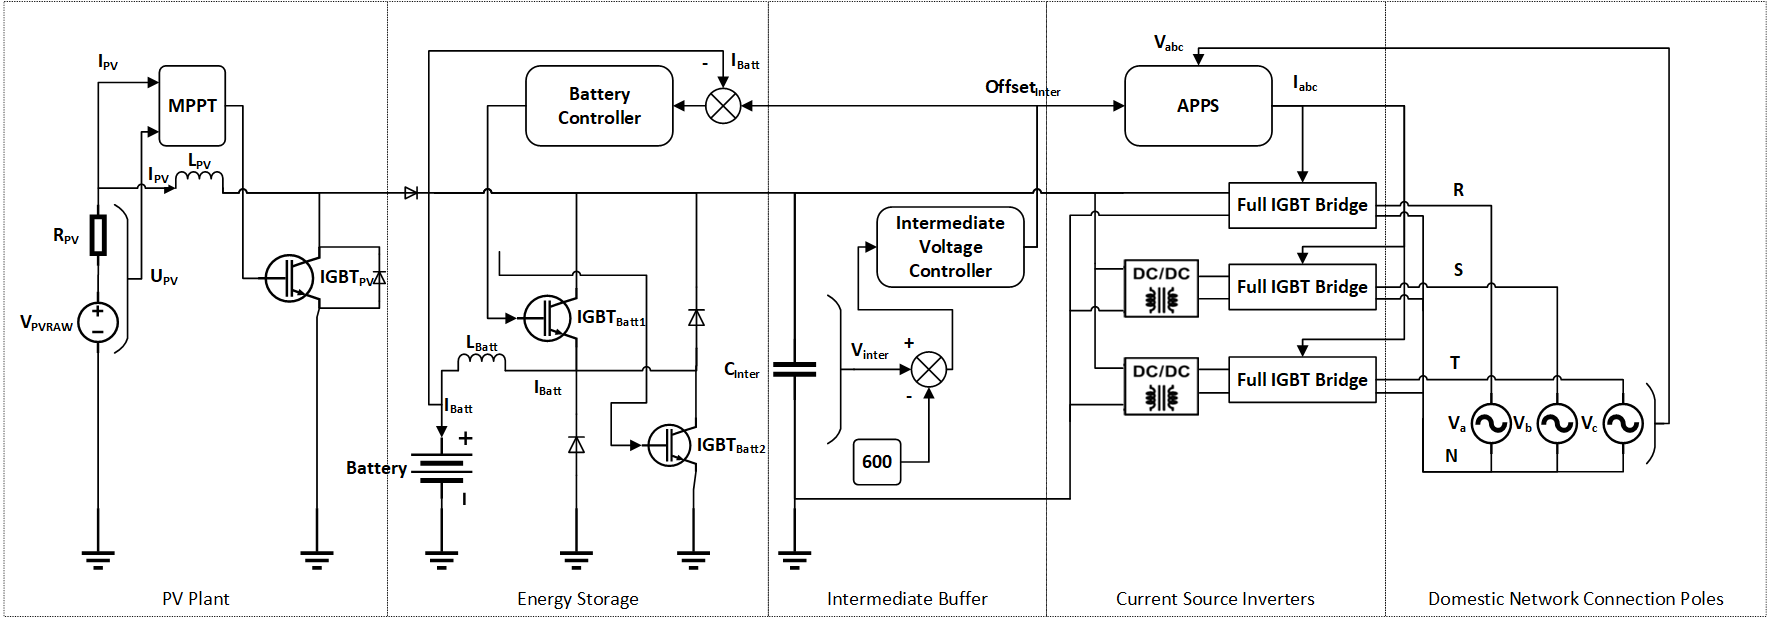
\includegraphics[width=1.5\textwidth,angle=-90]{Unblance_EPS_Pics/PowerTopology_full.png}
        \caption{asd}
        \label{fig:inv}
        \end{figure}

        Of course there is a possibility that there is no renewable power available for a longer period of time and the battery completely looses its charge. In this case the system should work merely with the power of the connection point but with zero energy balance. This states to operate two controller with semi-opposite control goals. The optimization based controller requires current injection while the intermediate voltage controller (Figure \ref{fig:inv}) keeps the inverters energy balance.\emph{ Although for this operation some of the control's performance should be sacrificed, unbalance compensation could be achieved even without external renewable power, and energy storage at a minimum power requirement.}

        \subsubsection{Measurements from a real unbalanced network}\label{VUB:sec:Measurement}

            The measurements took place at the campus building's power electronics laboratory, where a common 400\,V connection point was investigated as the behaviour of the network. The three phase 230\,V line-to-ground voltages has been transformed to 6\,V to be effectively measurable in time domain with high performance NI-USB DAQ on 10\,ksample/s. Because of the limited computational capacity only a 10 second measurement was made in every hour.  The measurements then has been merged and smoothed to eliminate the inter-measurement transients.\\
            Afterwards, the measurement data has been used as the input of a micro-grid segment of the Matlab/Simulink model, to test the controller and inverters structure's performance in quasi-realistic circumstances. The controllers performance on the simulated microgrid's network loss reduction can be observed on Figure \ref{fig:compare_power} and Figure \ref{fig:u_inter}. The measurement output is connected to a modeled three phase load and network system, consisting of symmetrical loads and network segments between them. Further artificial load unbalance is not necessary since the network's unbalance is already present. This structure enables to show that any point the inverter is connected, could restore power quality with a certain degree such unbalance compensation at this case. The future plan is to set up multiple devices on different connection points.

\section{Discussion}\label{VUB:sec:Discussion}

%write stuff here..

    \subsection{Dynamical simulation based experiments}\label{VUB:sec:Results}
		
    In order to be able to investigate the proposed optimization based unbalance reduction control structure with the three phase inverter on a low voltage local grid, all the elements of this complex electrical system (including the photovoltaic source, the inverter, the battery and the nonlinear local grid with different types of loads) has been modeled in Matlab/Simulink environment. The primary aim of the simulation based experiments were to serve as a proof of concept for the proposed complex control structure.

    \subsection{Performance analysis}\label{VUB:sec:Performance}

    The aim of performance analysis is twofold. First of all, the proposed voltage unbalance indicator has to be investigated in the control structure as the cost function of the optimization based controller, and on the other hand, the control structure itself has to be exposed against engineering expectations.


            The results of the first experiment can be seen in Figure \ref{fig:compare_asym_PV} where the geometrical norm \ref{equ:geom} has been used as the voltage unbalance indicator and the cost function for the optimizer.  The dashed line represents the examined low voltage local network's unbalance norm ($G$) without the proposed controller implemented in the inverter unit of the domestic powerplant while the solid line represents the compensated network's norm value. The performance of the controller with this norm is apparent, it was able to decrease the network voltage unbalance by approximately 85 \%. In this experimental setup the controller has enough input energy due to the batteries and the available solar power.

            \begin{figure*}[ht]
            \centering
            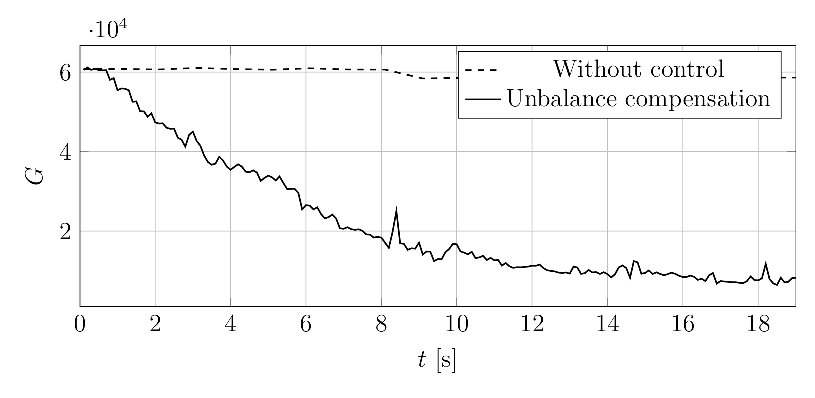
\includegraphics[width=0.95\textwidth]{Unblance_EPS_Pics/UnbalRedComp_JCP-figure3.eps}
            \caption{Unbalance reduction control system performance with half charged battery and photovoltaic power source available. The underlying unbalance norm is the geometrical one ($G$) in this experiment. After starting the controller at $t=0.1s$ the unbalance measure $G$ of the network significantly decrease.}
            \label{fig:compare_asym_PV}
            \end{figure*}

            \begin{figure*}[ht]
            \centering
            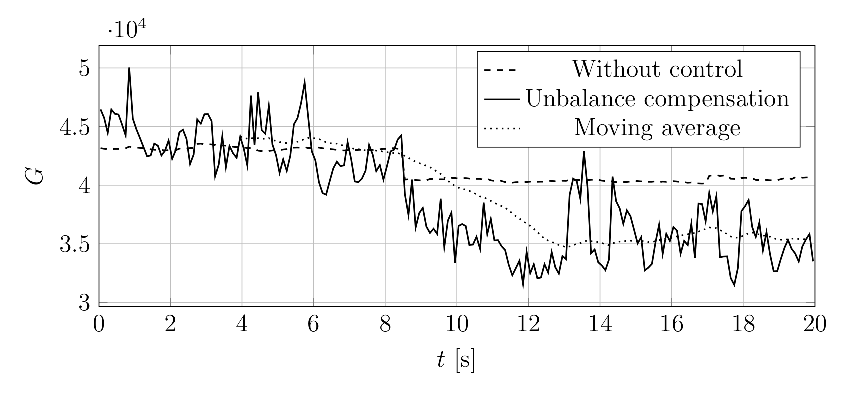
\includegraphics[width=0.95\textwidth]{Unblance_EPS_Pics/UnbalRedComp_JCP-figure4.eps}
            \caption{Unbalance reduction control system performance without battery and renewable source (zero energy balance operation). The performance reduction is clearly observable compared to the case when external power source is available (Figure \ref{fig:compare_asym_PV}), but as result the voltage unbalance indicator $G$ reduced by the average value of 14.78\%.}
            \label{fig:compare_asym}
            \end{figure*}

            A slightly more challenging situation is investigated in Figure \ref{fig:compare_asym} where the controller had had to operate without photovoltaic source and batteries. This is called zero moving average balance operation mode when the energy obtained from the network is reinjected in such a way that the unbalance indicators decrease. It can be seen that the performance of the controller is modest than that of Figure \ref{fig:compare_asym_PV}, but it is still acceptable.

      \subsubsection{Robustness analysis}\label{VUB:sec:Robustness}

            The robustness of the proposed control structure is an important qualitative property with respect to the time dependent loads present on the network. The robustness of the proposed controller had to be tested via simulation when different types of loads (inductive, capacitive, resistive) had been varied in step changes representing the on/off switching the different types of household appliances (motors, switching mode power supplies, electric heaters, etc.). In the experiment depicted in Figure \ref{fig:robustness}, a load change has been introduced to the network in every 15 seconds causing the voltage unbalance to jump to a different value (measured in the geometrical norm \ref{equ:geom}). As it can be seen in the figure the controller successfully compensates the unbalance after each transient.

              \begin{figure*}[ht]
            \centering
            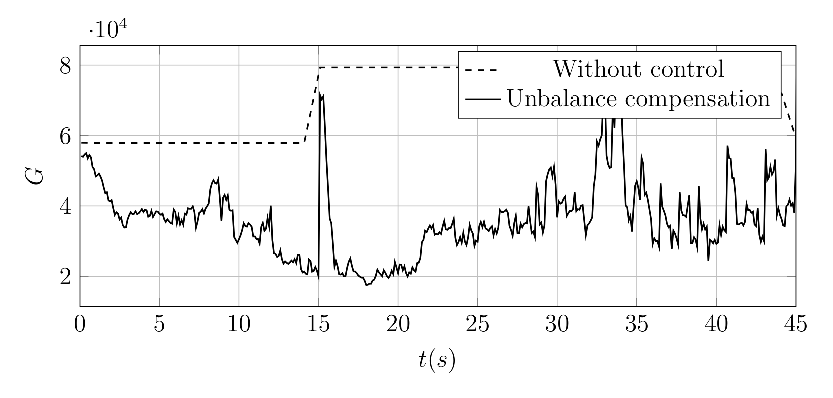
\includegraphics[width=0.95\textwidth]{Unblance_EPS_Pics/UnbalRedComp_JCP-figure5.eps}
            \caption{Robustness analysis with respect to step type changes in the network load (and voltage unbalance). The unbalance reduction controller successfully compensates the changes in the network voltage unbalance norm ($G$) value.}
            \label{fig:robustness}
            \end{figure*}

    \subsection{Environmental effect}\label{VUB:sec:Environment}

    The favorable effects of the proposed unbalance reduction control algorithm , i.e. increase power quality not only at the connection point but in the whole low voltage transformer area, which causes a reduction of the effective power loss and the reduction in the CO${}_2$ emission.

        \subsubsection{Power loss reduction on the network}\label{VUB:sec:Powerloss}

             Network loss reduction due to the unbalance reduction compensation control is investigated on Figure \ref{fig:compare_power} where the simulation experiment was carried out in the circumstance when the renewable source was not shut down (e.g. insufficient amount of sunlight) and additionally the battery was drained completely  \cite{Neukirchner2015}, \cite{neukirchner2015examination}.

            \begin{figure*}[ht]
            \centering
            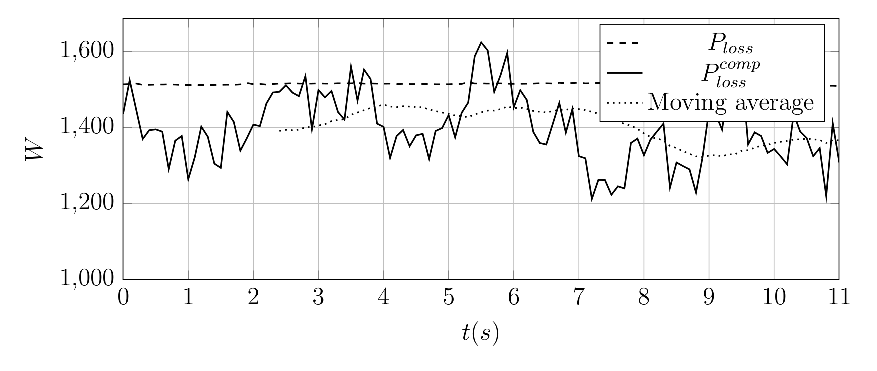
\includegraphics[width=0.95\textwidth]{Unblance_EPS_Pics/UnbalRedComp_JCP-figure6.eps}
            \caption{Compensation control's loss reduction during zero energy balance operation on the modeled network, where $P_{loss}$ indicates the effective power losses and $P^{comp}_{loss}$ effective power losses during control of the network. As result the network losses reduced by mean $6.5\%$.}
            \label{fig:compare_power}
            \end{figure*}

            The results show that despite of the negative cross effects of the intermediate voltage controller and the unbalance reduction controller it was possible to find the trade-off between the control goals of the different controllers (maintain zero energy balance for the inverter and decrease the unbalance on the network). The estimated loss reduction in the experimental setup is 6.5\%.

            \begin{figure*}[ht]
            \centering
            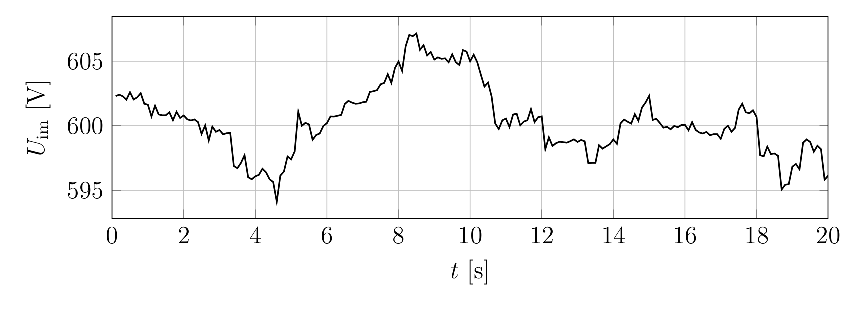
\includegraphics[width=0.95\textwidth]{Unblance_EPS_Pics/UnbalRedComp_JCP-figure7.eps}
%                  %\pgfplotsset{every tick label/.append style={font=\tiny},legend style={at={(1,1)},anchor=north east}}
%                 \pgfplotsset{every tick label/.append style={font=\normalsize}}
%                 \begin{tikzpicture}
%                 \begin{axis}[
%                     width=\textwidth,
%                     height=5cm,
%                     xlabel = {$t$~[s]},
%                     ylabel = {$U_{\textnormal{im}}$~[V]},
%                     grid=major,
%                     xmin=0,
%                     xmax=20,
%                     %ymin=0,
%                     ]
%                     \addplot[thick] table {netw_plot/U_inter.dat};
%                     %\legend{\scriptsize$U_{intermediate}$}
%                     \end{axis}
%                  \end{tikzpicture}
                 \caption{Intermediate puffer capacitance's voltage within boundaries ($600\pm10$\,V), during zero energy balance operation mode of the voltage unbalance compensation controller. $U_{\textnormal{im}}$ indicates intermediate the capacitance's voltage.}
                 \label{fig:u_inter}
                \end{figure*}

%        \subsubsection{Malfunction rejection}
%
%            asd

        \subsubsection[CO2 footprint]{CO$_2$ footprint}\label{VUB:sec:CO2}

            The fact that this controller enables the reactive power reduction has a favourable consequence, i.e. the power loss or equivalently CO$_2$ emission and the carbon footprint can also be decreased. The estimated environmental effects of voltage asymmetry compensation can be calculated. Let us assume 3000\,kWh for the yearly electric energy consumption an average household and $9.173\%$ for the loss of the distribution network at 2013 \cite{MVM2013} and $7.654\%$ at 2018 \cite{MVM2018}. Using the controller the losses on the simulated network are reduced by 6.5\%. The calculation follows \ref{eqn:co_emission}:

            \begin{equation}
                \label{eqn:co_emission}
                \begin{array}{rcl}
                 P_{loss}&=&3000\,\textnormal{kWh}\cdot7.654\%\\
                P^{comp}_{loss}&=&3000\,\textnormal{kWh}\cdot(7.654\cdot0.93)\%\\
                 \Delta P_{loss}&=&P_{loss}-P^{comp}_{loss}\\
                 \end{array}
                \end{equation}

            where $P_{loss}$ is the assumed network loss per household and $P^{comp}_{loss}$ is s the assumed network loss with unbalance compensation control and $\Delta P_{loss}$ is the saved energy. According to \ref{eqn:co_emission}, unbalance compensation results in an energy savings of 19.26 kWh in 2013 and 16.07 kWh in 2018. Taking into account the proportion of power currently generated by fossil fuels (coal 17.3\%, gas 38.3\% at 2013 \cite{MVM2013}, \cite{gorbe2012reduction} and coal 13.1\%, gas 51.4\% at 2018 \cite{MVM2018}) and the rate of $\textnormal{CO}_2$ emission during electric energy production (1,000\,g/kWh from coal and 430\,g/kWh from gas), it can be concluded that voltage unbalance compensation could reduce $\textnormal{CO}_2$ emissions by 6504.9\,g a year in 2013 and 5656.96\,g in 2018 in an average household. Note that this result reflect only the proof of concept, due the neglected power losses of the inverter and the artificial load of the network.
						
						%2105.17+3551.79

\section{Conclusion}\label{VUB:sec:Conclusion}

    Currently used measures of voltage unbalance (see section \oldref{BASICUNB:sec:DefinitionsofUNB}) has been extended in this chapter with a new norm candidate, namely a geometrical norm, where the magnitude of voltage unbalance are evaluatad by the symmetrical difference of the voltage phasor triangles. It is more demanding from the computational point, of view but has an interesting feature namely it checks electrical asymmetry, i.e. the norm of a $\pm120$ degree  rotated version of the ideal three-phase phasor is zero in the geometrical sense.\\
    This way, the defined norm is applied as a cost function in the asymmetry reducing controller structure utilizing an asynchronous parallel pattern search (APPS) algorithm also presented in the thesis. Simulations, performed in Matlab/Simulink environment show that the geometrical based indicator can serve as a basis of further research. The suggested controller structure enables the residential users owning a grid synchronized domestic power (renewable) plant to reduce voltage unbalance measurable at the connection point. The fundamental element of the system is a modified three phase inverter that is capable of the asymmetric current injection of any current waveforms to the network, via decoupled bi-directional DC-DC converters. The optimization-based control algorithm injects the available energy (as current waveform) in such a way, that the voltage unbalance decreases. This is an optimization problem which is constrained by the available renewable energy supplied by the power plant, or energy storage unit.\\
    The control structure has been tested on a low voltage network model in a dynamical simulation environment consisting of the models of the electrical grid, a domestic power plant, an asymmetrical inverter circuit, and different types of loads. Different simulation experiments has been run for each norm and for both the power constrained and unconstrained case. The preliminary results show that this structure can serve as a residential level voltage quality improvement method for the three phase low voltage network also indirectly reduces the CO${}_2$ emission due facilitating more effective energy usage.

%\section{Voltage unbalance compensation with optimization based control algorithm and asymmetrical inverter structure}
%
%    Based on the proposed measures of voltage unbalance it is possible to formulate some power quality related aims, or demands for the domestic size generator units as follows.
%
%    \subsection{Problem statement}
%
%    The voltage and current unbalance presents in the three phase low voltage transformer area causes additional power loss inside the medium voltage/low voltage transformer and in the transportation line wires too. It also has undesired effects in certain three phase loads, mainly rotating machines where it causes torque reduction and pulsating torque effect. Large scale unbalance can activate automatic protection functions of electricity dispatch system causes power outage. This is unpleasant for the customers and adds maintenance cost to the service provider. These negative effects lower the electric power quality and rises the cost of electrical energy and rises the carbon footprint of our everyday life. Our aim to develop a three phase instrumentation, which can compensate these undesirable effects, lower or eliminate the voltage and current unbalance to lower the power losses and the CO${}_2$ emission and increase power quality not only at the connection point but in the whole low voltage transformer area. \emph{It is important to note, that this power quality improvement can be achieved without any significant added cost.} The aim is to integrate this function into an existing three phase photovoltaic inverter device connected to the low voltage grid, and the created complex energetic system is able to inject the renewable energy to the transportation network, can store the electrical energy from stochastic renewable sources in electrical vehicle batteries or feed the grid from the charged batteries in energy deficit and high demand simultaneous situations. Our new added value the integrated control algorithm which can highly lower or eliminate the observed unbalance of the network.
%
%    \subsection{Control problem}
%
%    The above problem statement partially specifies the solution space together with the solution method. The system of interest is the power grid with all the stochastic and nonlinear phenomena present in it. The input to the system is the current signals (one current in the single phase case and three in the three phase setup), which are naturally constrained by the available energy of the household - stored in a battery pack or momentarily generated by the wind or solar generator unit. The response of the system can be either the current or the voltage measured at the connection point of the inverter unit, however, the general legal regulations only allow voltage measurement for consumers. The difficulty of the control problem comes from the fact, that there are no mathematically tractable models of the network can be generated because of its unpredictable and nonlinear features. This means, that only black-box methods can be applied for this system.
%
%    For the control aim it is a natural choice to minimize the actual voltage unbalance of the low voltage local transformer area measured (or calculated) at the connection point of the inverter. Several optimization based methods are available for such kind of optimal control problems, e.g.  \cite{gorbe2012reduction} where the only bottleneck is the computational efficiency since the impemented controller has to run on the commercial inverter's hardware (digital singal processor unit).
%
%    \subsection{Asymmetrical inverter structure}
%
%    \textcolor{blue}{
%        The renewable energy injection is realized increasingly directly to the three phase low voltage grid in domestic size photovoltaic power plants too. This can reduce the voltage and current unbalance caused by the stochastic power production of wind and solar sources. More and more manufacturers produce three phase grid synchronized inverters from 5\,kW size. These equipments implement accurate symmetrical current feed with a standard three phase full bridge structure consists of six Isolated Gate Bipolar Transistors (IGBT). This is a cost effective standard structure suitable for symmetric harmonic current injection. It has limited capacities to inject not totally symmetric 3 phase current time functions, but Kirchhoff's current law permits only constant zero-sum current time functions injected with this structure. There are examples with this type of asymmetric current injections in the literature \cite{lee2010new}.}
%
%         %ide kellene a hivatkozás arra a cikkre, amit mutattál, ahol nem 120 fokosak a vektorok a fazor diagrammon, de az összegük 0
%    \textcolor{blue}{
%        This type of current injections has limited compensation capacity and this is not enough in  most asymmetric production and load cases. In our case we need more general, not specific asymmetric current waveforms, because the proposed control aim assumes the ability of injecting non zero-sum currents. This needs special inverter design structure. We need zero line connection for the differential current. One of the possible solution is to use 3 different full bridge single phase current inverters to supply each phase of low voltage transportation lines \cite{Patnaik2013topologies}. But in this case we need galvanic isolations of these single phase inverters in the output, or in the DC input size.}
%
%        %ide tegyük be hivatkozásnak: "Sushree Sangita Patnaik ., Anup Kumar Panda:Three-level H-bridge and three H-bridges-based three-phase four-wire shunt active power filter topologies for high voltage applications"
%    \textcolor{blue}{
%        This isolation can be reached  with using isolation transformers in the supply side. But we would like to use it a complex energetic system with specific inside true DC bus system feeded from Photovoltaic panel or batteries. We have to isolate  at least 2 full bridges with two way DC-DC converters. This can complicate the physical realization but easy to simulate with two controlled power source. Other possible easy to realize solution to isolate the full bridge outputs  connected to three phase lines with isolating transformers. It is recommended for operating and electric shock protection reasons too (Figure \ref{fig:asymminvwithgalvanic transformer}).Our distant aim to compensate other operational type line failures, such zero current appearing. This isolation method doesn't allow to produce CD current components, thats why we are looking for other design. Possible elegant solution to supplement the standard three phase inverter design with a fourth half bridge for Zero line, building a specific four leg inverter design \cite{Ninad2014control}.}
%
%        %ide tegyük be hivatkozásnak: "Nayeem Ahmed Ninad ., Luiz Lopes:Per-phase vector control strategy for a four-leg voltage source inverter operating with highly unbalanced loads in stand-alone hybrid systems"
%    \textcolor{blue}{
%        Only drawback of this solution is the complex difficult control method of the half bridges, to keep the current sum in zero values in each moment, and to provide the correct current paths inside the inverter. This structure has the lowest production cost, but in the phase of proofing the asymmetry compensation we chose the DC-DC isolated  full bridge design for simulation purpose because of the simple control during simulation.}
%    \textcolor{blue}{
%        As a further generalization step, the injection of no harmonic current shapes will be necessary in order to decrease the extant Total Harmonic Distortion (THD) of the network. These expectations yield an inverter with new structure suitable for arbitrary current injections without limitations. The design lends similar elements like in \cite{gorbe2012reduction} by means of battery charge, renewable power point tracking, intermediate voltage, and IGBT bridge control, but in this case the problem requires a three phase solution for the voltage unbalance reduction. The applied structure based on a full bridge IGBT structure used in single phase current injection. Three different IGBT full bridge were connected at the output point, thus our structure has three phase and neutral connection too, to carry out any current form. The disadvantage of this structure is that it needs 12 IGBTs in the output stage as opposed to the 6 IGBTs needed for a classical full bridge structure and needs three galvanically isolated direct current (DC) voltage source for feeding.}
%    \textcolor{blue}{The other standard elements, that the inverter design consists:}
%
%
%
%        \begin{itemize}
%            \item\textcolor{blue}{ Standard maximum power point tracking (MPPT) input stage, to inject the maximum available power from the renewable source to the intermediate voltage capacitor with a simple controlled boost converter}
%            \item\textcolor{blue}{ A half bridge current controller to charge or deploy the battery pack connected to the complex energetic system for energy storage and energy unbalance compensation}
%            \item\textcolor{blue}{ Intermediate voltage controller}
%            \item\textcolor{blue}{ Universal three phase output stage with 3 single phase full bridge IGBT current injector and 2 high current DC-DC converter}
%        \end{itemize}
%    \textcolor{blue}{
%        This is suitable to inject any necessary current shape to the low voltage three phase grid connection even DC currents too. Later a power loss and production cost analysis will be necessary if the built structure will be suitable for asymmetric compensation of low voltage transformer area.}
%
%        %\begin{figure*}[ht]
%%            \centering
%%            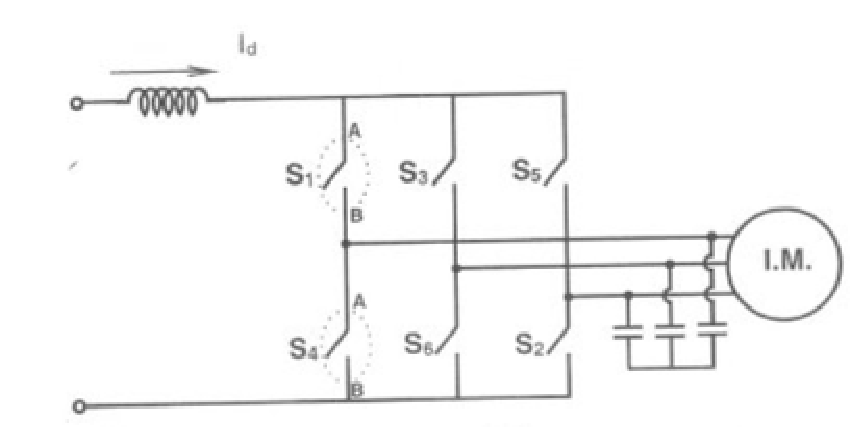
\includegraphics[width=0.95\textwidth]{standard_inverter.eps}
%%            \caption{\textcolor{blue}{Standard symmetrical current inverter design, implies 6 IGBT current injector with serial inductance. }}
%%        \label{fig: symminv}
%%        \end{figure*}
%
%        %\begin{figure*}[ht]
%%            \centering
%%            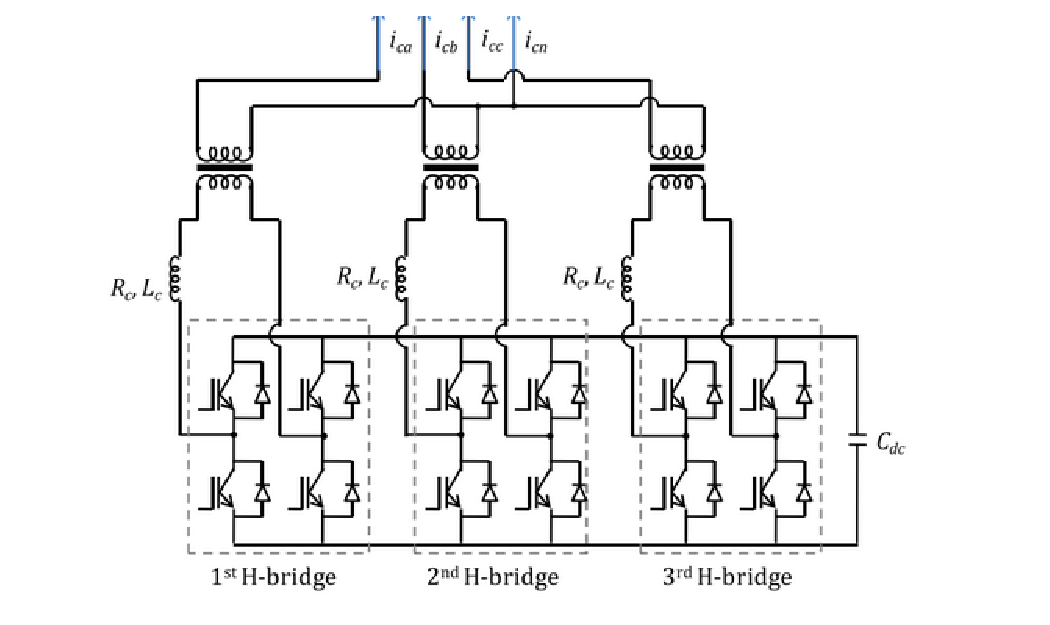
\includegraphics[width=0.95\textwidth]{isolated_inverter.eps}
%%            \caption{\textcolor{blue}{Asymmetrical inverter design with three separated H-bridges.}}
%%        \label{fig: asymminvwithDCgalvanic transformer}
%%        \end{figure*}
%
%\begin{figure}[h]
%          \begin{center}
%                \begin{circuitikz}[scale=.5, european] %% => Itt ne állíts a skálát, inkább a figure-nél!%%
%                %\draw[help lines] (0,0) grid (16,40);
%
%                \draw%[color=magenta]
%                    %% híd
%                    (0,0) to[C=$C_{intermediate}$] (0,38)
%                    (0,0) to[short] (10,0)
%                    (6,0) node[nigbt, anchor=E](nigbt33){}
%                    (nigbt33.E) node[circ]{}
%
%                    (10,8) node[nigbt, anchor=E,xscale=-1](nigbt32){}
%
%                    (6,8) node[nigbt, anchor=E](nigbt31){}
%                    (nigbt33.C) to[short] (nigbt31.E)
%
%                    (10,0) node[nigbt, anchor=E, xscale=-1](nigbt34){}
%                    (nigbt34.C) to[short] (nigbt32.E)
%
%                    (nigbt32.C) to[short] (10,12)
%                    (nigbt31.C) to[short,-*] (6,12)
%                    (4,12) to[short] (10,12)
%                    (4,12) to[short,-*] (4,38)
%
%
%                    %%trafó
%                    (7,6) node[transformer,rotate=90,transform shape,american](T3){}
%                    (T3.B1) to[short,-*] (6,7.05)
%                    (T3.B2) to[short,-*] (10,7.05)
%                    (T3.A1) to[short] (7,4)
%                    (7,4) to[short,-o] (13,4) node[anchor=west] {$N$}
%                    (T3.A2) to[short,-o] (13,4.95) node[anchor=west] {$T$}
%                    ;
%
%                    \draw%[color=blue]
%                    %% híd
%                    (3,13) to[short,*-] (10,13)
%                    (6,13) node[nigbt, anchor=E](nigbt23){}
%                    (nigbt23.E) node[circ]{}
%
%                    (10,21) node[nigbt, anchor=E,xscale=-1](nigbt22){}
%
%                    (6,21) node[nigbt, anchor=E](nigbt21){}
%                    (nigbt23.C) to[short] (nigbt21.E)
%
%                    (10,13) node[nigbt, anchor=E, xscale=-1](nigbt24){}
%                    (nigbt24.C) to[short] (nigbt22.E)
%
%                    (nigbt22.C) to[short] (10,25)
%                    (nigbt21.C) to[short,-*] (6,25)
%                    (4,25) to[short,*-] (10,25)
%
%
%
%
%                    %%trafó
%                    (7,19) node[transformer,rotate=90,transform shape,american](T2){}
%                    (T2.B1) to[short,-*] (6,20.05)
%                    (T2.B2) to[short,-*] (10,20.05)
%                    (T2.A1) to[short] (7,17)
%                    (7,17) to[short,-*] (12,17)
%                    (T2.A2) to[short,-o] (13,17.95) node[anchor=west] {$S$}
%                    ;
%
%                    \draw%[color=cyan]
%                    %% híd
%                    (3,26) to[short] (10,26)
%                    (3,26) to[short,-*] (3,0)
%
%                    (6,26) node[nigbt, anchor=E](nigbt13){}
%                    (nigbt13.E) node[circ]{}
%
%                    (10,34) node[nigbt, anchor=E,xscale=-1](nigbt12){}
%
%                    (6,34) node[nigbt, anchor=E](nigbt11){}
%                    (nigbt13.C) to[short] (nigbt11.E)
%
%                    (10,26) node[nigbt, anchor=E, xscale=-1](nigbt14){}
%                    (nigbt14.C) to[short] (nigbt12.E)
%
%                    (nigbt12.C) to[short] (10,38)
%                    (nigbt11.C) to[short,-*] (6,38)
%                    (0,38) to[short] (10,38)
%
%
%                    %%trafó
%                    (7,32) node[transformer,rotate=90,transform shape,american](T1){}
%                    (T1.B1) to[short,-*] (6,33.05)
%                    (T1.B2) to[short,-*] (10,33.05)
%                    (T1.A1) to[short] (7,30)
%                    (7,30) to[short] (12,30)
%                    (12,30) to[short,-*] (12,4)
%                    (T1.A2) to[short,-o] (13,30.95) node[anchor=west] {$R$}
%                    ;
%                %%
%                \end{circuitikz}
%                \caption{\textcolor{blue}{Simplified asymmetrical inverter design employing three galvanically isolated H-bridges with transformers for DC-DC isolation substitution.}}
%                \label{fig: asymminvwithgalvanic transformer}
%          \end{center}
%    \end{figure}
%
%        %\begin{figure*}[ht]
%%            \centering
%%            \includegraphics[width=0.95\textwidth]{isolated_only_inverter.eps}
%%            \caption{\textcolor{blue}{Simplified asymmetrical inverter design employing three galvanically isolated H-bridges with transformers for DC-DC isolation substitution.}}
%%        \label{fig: asymminvwithgalvanic transformer}
%%        \end{figure*}
%
%
%        \begin{figure*}[ht]
%        \centering
%        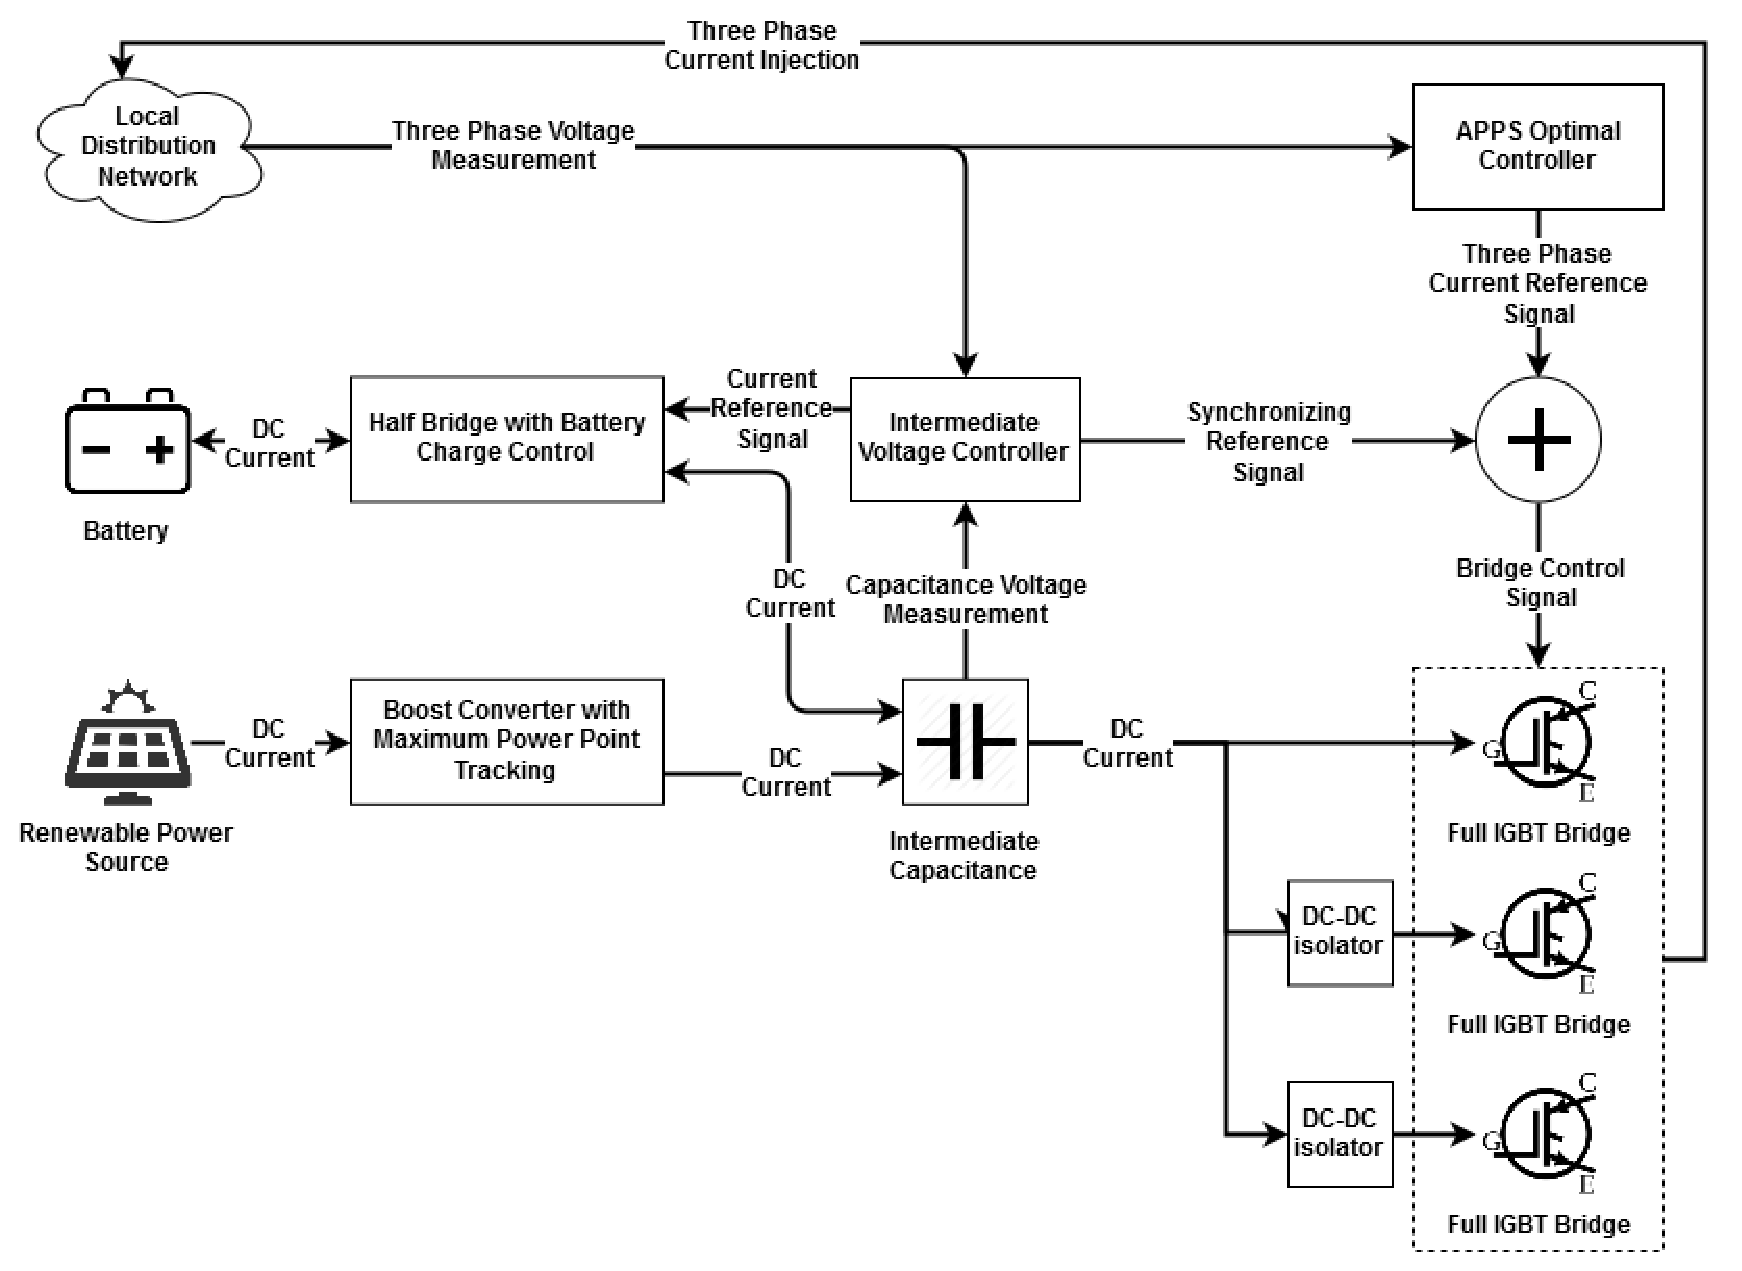
\includegraphics[width=0.95\textwidth]{Unblance_EPS_Pics/inverter.eps}
%        \caption{\textcolor{blue}{The asymmetrical inverter design, which applies three single phase full bridge IGBT current injector to create the injected asymmetrical current shapes for voltage unbalance compensation. }}
%        \label{fig:inv}
%        \end{figure*}
%
%    \textcolor{blue}{
%        Of course there is a possibility that there is no renewable power available for a longer period of time and the battery completely looses its charge. In this case the system should work merely with the power of the connection point but with  zero energy balance. This states to operate two controller with semi-opposite control goals. The optimization based controller requires current injection while the intermediate voltage controller (Figure \ref{fig:inv}) keeps the inverters energy balance. Although for this operation some of the control's performance should be sacrificed, unbalance compensation could be achieved even without external renewable power, and energy storage at a minimum power requirement.}
%        %\subsubsection{The necessity of switching the control off}
%%
%%                \textcolor{blue}{Inverter lea\'all\'it\'as\'anak sz\"uks\'egess\'ege.}
%
%%
%        The renewable energy injection is realized increasingly directly to the three phase low voltage grid in domestic size photovoltaic power plants too. This can reduce the voltage and current unbalance caused by the stochastic power production wind and solar sources. More and more manufacturers produce three phase grid synchronized inverters from 5\,kW size. These equipments implement symmetrical power feed with a standard three phase full bridge structure consists of six Isolated Gate Bipolar Transistors (IGBT). This is a cost effective standard structure suitable for symmetric harmonic current injection, but Kirchhoff's current law permits only constant zero-sum current time functions injected with this structure. The proposed control aim assumes the ability of injecting non constant zero-sum currents. As a further generalization step, the injection of no harmonic current shapes will be necessary in order to decrease the extant Total Harmonic Distortion (THD) of the network. These expectations yield an inverter with new structure suitable for arbitrary current injections without limitations. The design lends similar elements like in \cite{gorbe2012reduction} by means of battery charge, renewable power point tracking, intermediate voltage, and IGBT bridge control, but in this case the problem requires a three phase solution for the voltage unbalance reduction. The applied structure based on a full bridge IGBT structure used in single phase current injection. Three different IGBT full bridge were connected at the output point, thus our structure has three phase and neutral connection too, to carry out any current form. The disadvantage of this structure is that it needs 12 IGBTs in the output stage as opposed to the 6 IGBTs needed for a classical full bridge structure and needs three galvanically isolated direct current (DC) voltage source for feeding. \\
%        The other standard elements, that the inverter design consists:
%        \begin{itemize}
%            \item Standard maximum power point tracking (MPPT) input stage, to inject the maximum available power from the renewable source to the intermediate voltage capacitor with a simple controlled boost converter
%            \item A half bridge current controller to charge or deploy the battery pack connected to the complex energetic system for energy storage and energy unbalance compensation
%            \item Intermediate voltage controller
%            \item Universal three phase output stage with 3 single phase full bridge IGBT current injector and 2 high current DC-DC converter
%        \end{itemize}
%        This is suitable to inject any necessary current shape to the low voltage three phase grid connection even DC currents too. Later a power loss and production cost analysis will be necessary if the built structure will be suitable for asymmetric compensation of low voltage transformer area.
%
%        %\begin{figure*}[ht]
%%        \centering
%%        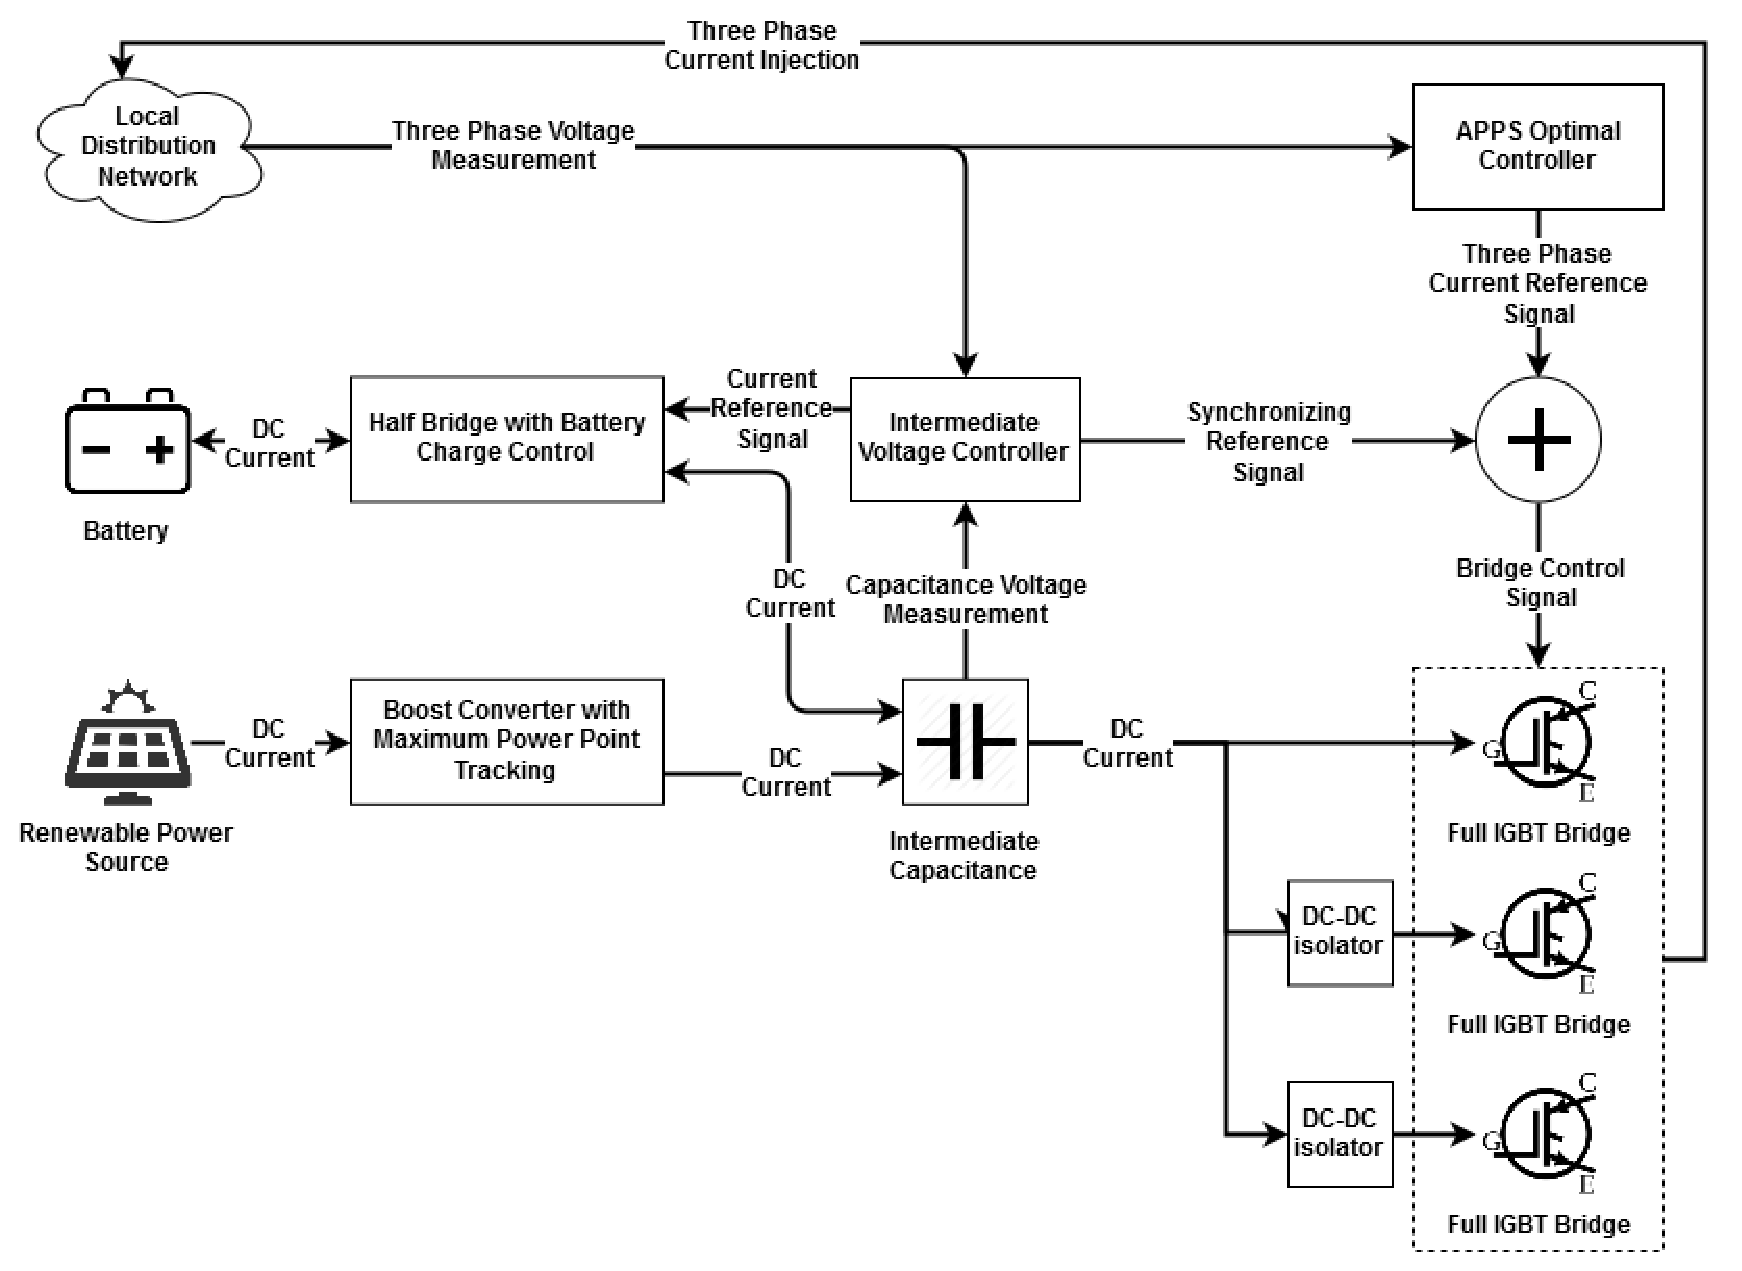
\includegraphics[width=0.95\textwidth]{Unblance_EPS_Pics/inverter.eps}
%%        \caption{The asymmetrical inverter design, which implies 3 single phase full bridge IGBT current injector to form the injected asymmetrical current shapes for voltage unbalance compensation. }
%%        \label{fig:inv}
%%        \end{figure*}
%%
%        Of course there is a possibility that there is no renewable power available for a longer period of time and the battery completely looses its charge. In this case the system should work merely with the power of the connection point but with  zero energy balance. This states to operate two controller with semi-opposite control goals. The optimization based controller requires current injection while the intermediate voltage controller (Figure \ref{fig:inv}) keeps the inverters energy balance. Although for this operation some of the control's performance should be sacrificed, unbalance compensation could be achieved even without external renewable power, and energy storage at a minimum power requirement.
%        %\subsubsection{The necessity of switching the control off}
%%
%%                \textcolor{blue}{Inverter lea\'all\'it\'as\'anak sz\"uks\'egess\'ege.}
%
%        \subsubsection{Measurements from a real unbalanced network}
%
%            The measurements took place at the Faculty's building, where a common 400\,V connection point was investigated as the behaviour of the network. The three phase 230\,V line-to-ground voltages has been transformed to 6\,V to be effectively measurable time domain with high performance NI-USB DAQ on 10\,ksample/s. Because of the limited computational capacity only a 10 second measurement was made in every hour.  The measurements then has been merged and smoothed to eliminate the inter-measurement transients.\\
%            Afterwards, the measurement data has been used as the output of a micro-grid segment of the Matlab/Simulink model, to test the controller and inverters structure's performance in quasi-realistic circumstances. The controllers performance on the simulated microgrid's network loss reduction can be observed on (Figure \ref{fig:compare_power}). The measurement output is connected to a modeled three phase load and network system, consisting of symmetrical loads and network segments between them. Further artificial load unbalance is not necessary since the network's unbalance is already present. This structure enables to show that any point the inverter is connected could serve as quality restoration such unbalance compensation at this case. Our future plan is to set up multiple devices on different connection points.
%
%
%
%    \subsection{Optimization based control algorithm}
%
%        \begin{figure*}[ht]
%        \centering
%        \includegraphics[width=0.95\textwidth]{Unblance_EPS_Pics/APPS_grey.eps}
%        \caption{\textcolor{blue}{The optimization algorithm implemented for current control. A one dimensional linear optimization step is being solved in each dimension of the six dimensional parameter space, iteratively.}}
%        \label{fig:APPS}
%        \end{figure*}
%
%        The problem is that, the exact mathematical relation is nonlinear because the nonlinear, and highly time variant loads of the network, we should use a control strategy to cope this nonlinear and time variant energy system. For this purpose we chose an asynchronous parallel pattern search method (APPS) which could be able to control our scenario.  We applied a variant of the gradient method that is a first-order optimization (minimization) algorithm for a multivariate function $f(x)$. The point $x(k)$ corresponding to the local minimum can be calculated from the negative gradient $\delta f(x)$, that gives the value and direction of the corresponding step in the parameter space. The next step is made in the direction of gradient with the proper sign. This sequence of steps, ideally, converges to local multivariate extreme value $x(k)$ of the function (\ref{eqn:contstruct1}).
%
%        \begin{equation}
%        \begin{array}{rcl}
%        \label{eqn:contstruct1}
%         x^{(k)}&=&x^{(k-1)}-t_k \nabla f(x^{(k-1)})\\
%         k&\in&\mathbb{N}\\
%         \end{array}
%        \end{equation}
%
%        The controlled electrical system is described by multivariate non-linear differential equations, the optimization of which is infeasible to derive using the differentiation of an error function. Therefore, the optimization methods based on direct differentiation are not applicable. In such cases, when high computational power is needed for performing long time-consuming simulations, the APPS method can utilized. The search pattern $p$ is based on the sampling of the error function (selected norm) on a "grid", and it corresponds to variables or subsets of variables in each point in the independent variable or parameter space easily. At the same time, the norm values at these points can be calculated independently if $\Delta k>0$, using (\ref{eqn:contstruct2}).
%        \begin{equation}
%        \label{eqn:contstruct2}
%        \begin{array}{rcl}
%         x^{(k+1)}&=&x^{(k)}+\Delta _kd_i \\
%         \mathrm{if}&&f(x^{(k)}+\Delta _kd_i) \leq f(x^{(k)})\\
%         k&\in&\mathbb{N}\\
%         \end{array}
%        \end{equation}
%
%        The parameter is  $x(k)\in R_n$, and the search pattern $p\in D={d_1,...d_n}$ is taken from a predefined finite set. In this case, the error function values should be calculated for each pattern $p$ in the set $D$. If the error function is not decreasing in any of the directions, then the step size should be reduced (e.g. by half). As the competing directions are different, if there is not enough computing power available for direction vector $p$, synchronization should not be maintained. In this case we are talking about the asynchronous case . In the case of our controller, an individual $p$ vector is defined for each output variable, and the optimization was performed in each direction asynchronously and shifted in time. Most likely, the error function has a single local minimum as a symmetric amplitude and phase values. Approaching the minimal value of norm, the controller uses adaptive increments that are proportional to the norm itself. Because of the complex interactions between the components of the controller, only one parameter is changed at a time, even if the values of the amplitude and phase components in specific time slot changes. The algorithm moves along the six axes of six separate time slots close to the local minimum of the error function.\\
%        Unlike other similar approaches, e.g. \cite{segui2007approach}, the explained optimal controller does not rely on a measured current signal but rather measuring and analysing the voltage unbalance via the proposed indicator and optimizes the voltage shape, the latter of which depends on the nonlinear distortion of the whole low-voltage transformer area and determines additional power losses. The controller's performance was compared to a non compensated network, and a network consisting synchronised symmetric power intake from a regular inverter.\\
%        In each iteration only one physical value is changing on the six dimensional parameter field, which consists of the three amplitude and three phase values. If the change effects with cost function reduction (the reference norm's normalised value), the controller holds the new value of amplitude or phase for the controlled current sources. The advantage of this controller structure that is not necessary to know the controlled value's behaviour well, like we could not determine the number and type of the other loads on the network \cite{Neukirchner2015}. There are however two disadvantages. First is the low speed of control, due to the several necessary iterations (depending on the circumstances) to find the optimal directions in the parameter space, and the serial nature of interventions and norm calculations. The second comes from the method itself since the controller may stuck in local minima.
%
%    %\subsubsection{Higher level control structure}
%%
%%            \begin{itemize}
%%            \item \textcolor{blue}{Norm\'al \'es z\'er\'o energimam\'erleg \"uzemm\'odok.}
%%            \item \textcolor{blue}{\"Uzemm\'od v\'altasok.}
%%            \end{itemize}
%
%\subsection{Discussion}
%    \subsubsection{Dynamical simulation based experiments}
%    In order to be able to investigate the proposed optimization based unbalance reduction control structure with the three phase inverter on a low voltage local grid, all the elements of this complex electrical system (including the photovoltaic source, the inverter, the battery and the nonlinear local grid with different types of loads) has been modeled in Matlab/Simulink environment. The primary aim of the simulation based experiments were to serve as a proof of concept for the proposed complex control structure.
%    \subsubsection{Performance analysis}
%    The aim of performance analysis is twofold. First of all, the proposed voltage unbalance indicator has to be investigated in the control structure as the cost function of the optimization based controller, and on the other hand, the control structure itself has to be exposed against engineering expectations.
%
%%     The first experiment is depicted in Figure \ref{fig:compare_asym_VEC}, where the vectorial based voltage unbalance indicator was used as the cost function of the optimization algorithm. The results are far not promising since the value of norm $N$ of the network starts to oscillate when the unbalance reduction controller is active. The cause of this behaviour is \textcolor{red}{WHAT?}
%%
%%             % V ==========================
%%            \begin{figure*}[h]
%%             \centering
%%                  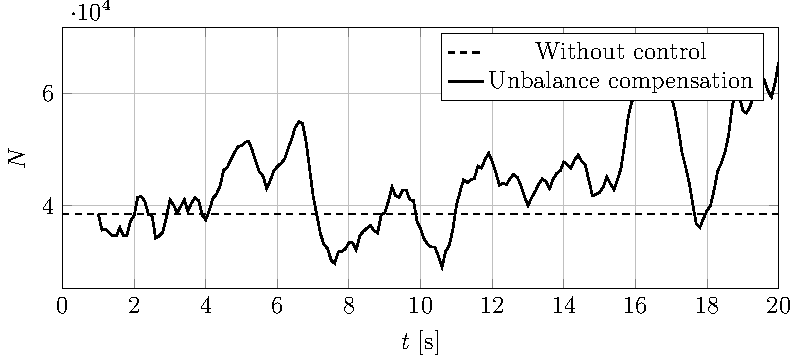
\includegraphics{UnbalRedComp_JCP-figure2.pdf}
%% %                 \pgfplotsset{every tick label/.append style={font=\normalsize}}
%% %                 \begin{tikzpicture}
%% %                 \begin{axis}[
%% %                     width=\textwidth,
%% %                     height=6cm,
%% %                     xlabel = {$t$~[s]},
%% %                     ylabel = {$N$},
%% %                     grid=major,
%% %                     xmin=0,
%% %                     xmax=20,
%% %                     %ymax=8000,
%% %                     %ymin=200,
%% %                     ]
%% %                     \addplot [dashed, thick] coordinates {(0,38520) (20,38520)};
%% %                     \addplot[thick] table {VEC_Measurements/VEC_orig.dat};
%% %                     \legend{Without control, Unbalance compensation}
%% %                     \end{axis}
%% %                  \end{tikzpicture}
%%                  \caption{Compensation control's voltage unbalance reduction, where $N$ indicates the calculation with the vectorial indicator value. The controller starts at $t=0.1s$ and starts oscillating towards unbalance.}
%%                  \label{fig:compare_asym_VEC}
%%                 \end{figure*}
%
%                The results of the first experiment can be seen in Figure \ref{fig:compare_asym_PV} where the geometrical norm \ref{equ:geom} has been used as the voltage unbalance indicator and the cost function for the optimizer.  The dashed line represents the examined low voltage local network's unbalance norm ($G$) without the proposed controller implemented in the inverter unit of the domestic powerplant while the solid line represents the compensated network'snorm value. The performance of the controller with this norm is apparent, it was able to decrease the network voltage unbalance by approximately 85 \%. In this experimental setup the controller has enough input energy due to the batteries and the available solar power.
%
%            % G ========================== +PV
%            \begin{figure*}[ht]
%            \centering
%            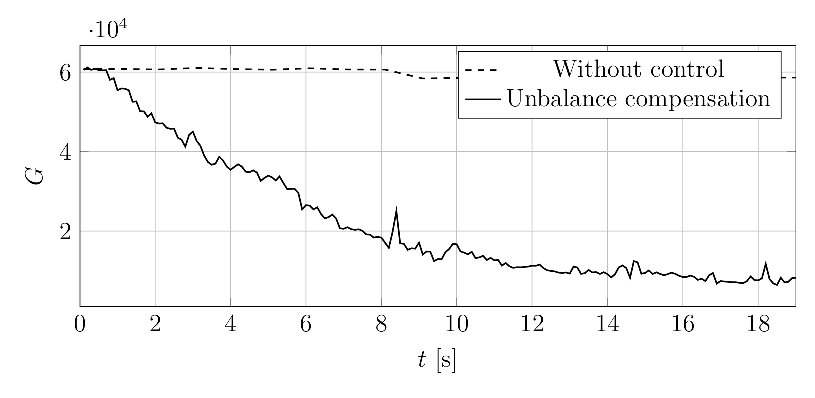
\includegraphics[width=0.95\textwidth]{Unblance_EPS_Pics/UnbalRedComp_JCP-figure3.eps}
%%                 %\pgfplotsset{every tick label/.append style={font=\tiny},legend style={at={(1,1)},anchor=north east}}
%%                 \pgfplotsset{every tick label/.append style={font=\normalsize}}
%%                 \begin{tikzpicture}
%%                 \begin{axis}[
%%                     width=\textwidth,
%%                     height=6cm,
%%                     xlabel = {$t$~[s]},
%%                     ylabel = {$G$},
%%                     grid=major,
%%                     xmin=0,
%%                     xmax=19,
%%                     %ymax=900,
%%                     %ymin=200,
%%                     ]
%%                     \addplot[dashed,thick] table {withPV/GEO_nocont_orig.dat};
%%                     \addplot[thick] table {withPV/GEO_orig.dat};
%%                     \legend{Without control, Unbalance compensation}
%%                     \end{axis}
%%                  \end{tikzpicture}
%                 \caption{Unbalance reduction control system performance with half charged battery and photovoltaic power source available. The underlying unbalance norm is the geometrical one ($G$) in this experiment. After starting the controller at $t=0.1s$ the unbalance measure $G$ of the network significantly decrease.}
%                 \label{fig:compare_asym_PV}
%                \end{figure*}
%
%                % G ========================== -PV
%            \begin{figure*}[ht]
%            \centering
%            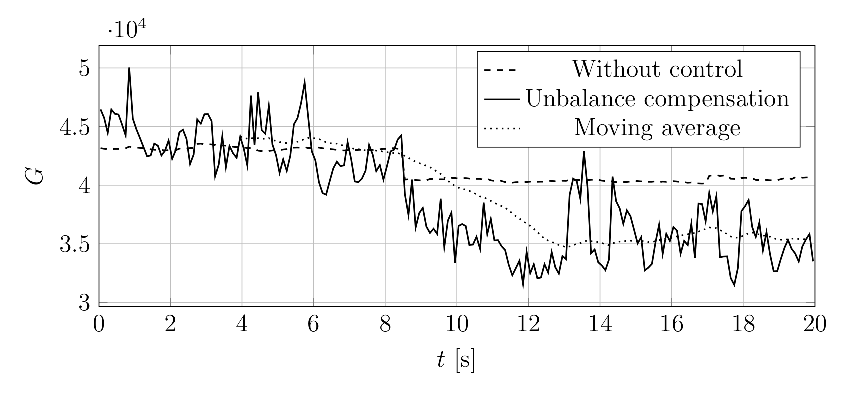
\includegraphics[width=0.95\textwidth]{Unblance_EPS_Pics/UnbalRedComp_JCP-figure4.eps}
%%                  %\pgfplotsset{every tick label/.append style={font=\tiny},legend style={at={(1,1)},anchor=north east}}
%%                 \pgfplotsset{every tick label/.append style={font=\normalsize}}
%%                 \begin{tikzpicture}
%%                 \begin{axis}[
%%                     width=\textwidth,
%%                     height=6cm,
%%                     xlabel = {$t$~[s]},
%%                     ylabel = {$G$},
%%                     grid=major,
%%                     xmin=0,
%%                     xmax=20,
%%                     %ymax=600,
%%                     %ymin=200,
%%                     ]
%%                     \addplot[dashed,thick] table {netw_plot_nocont/GEO_nocont_orig.dat};
%%                     \addplot[thick] table {netw_plot/GEO_orig.dat};
%%                     \addplot[dotted,thick] table {netw_plot/GEO_orig_mean.dat};
%%                     \legend{Without control, Unbalance compensation, Moving average}
%%                     \end{axis}
%%                  \end{tikzpicture}
%                 \caption{Unbalance reduction control system performance without battery and renewable source (zero energy balance operation). The performance reduction is clearly observable compared to the case when external power source is available (Figure \ref{fig:compare_asym_PV}), but as result the voltage unbalance indicator $G$ reduced by the average value of 14.78\%.}
%                 \label{fig:compare_asym}
%                \end{figure*}
%
%            A slightly more challangeing situation is investigated in Figure \ref{fig:compare_asym} where the controller had had to operate without photovoltaic source and batteries. This is called zero balance operation mode when the energy obtained from the network is reinjected in such a way that the unbalance indicators decrease. It can be seen that the performance of the controller is modest than that of Figure \ref{fig:compare_asym_PV}, but it is still acceptable.
%
%      \paragraph{Robustness analysis}
%
%            %\textcolor{magenta}{MACI}\\
%            %\textcolor{blue}{Robosztuss\'agi vizsg\'alat mind norm\'al mind zero balance esetre.}
%            The robustness of the proposed control structure is an important qualitative property with respect to the time dependent loads present on the network. The robustness of the proposed controller had to be tested via simulation when different types of loads (inductive, capacitive, resistive) had been varied in step changes representing represnting the on/off switching the different types of household appliances (motors, switching mode power supplies, electric heaters, stc.). In the experiment depicted in Figure \ref{fig:robustness}, a load change has been introduced to the network in every 15 seconds causing the voltage unbalance to jump to a different value (measured in the geometrical norm (\ref{equ:geom})). As it can be seen in the figure the controller successfully compensates the unbalance after each transient.
%
%              \begin{figure*}[ht]
%            \centering
%            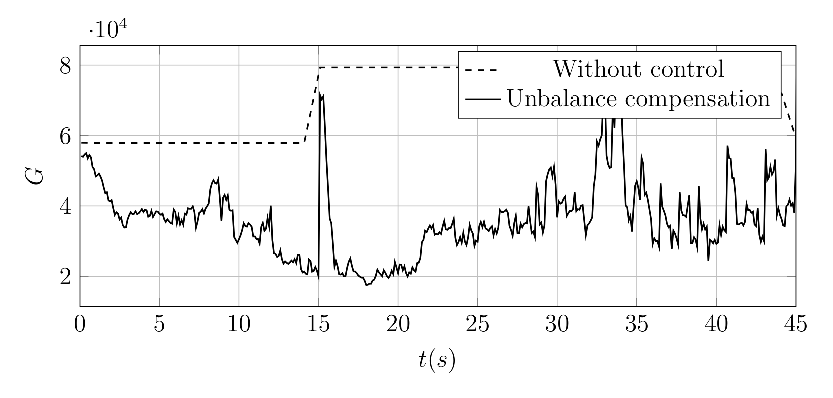
\includegraphics[width=0.95\textwidth]{Unblance_EPS_Pics/UnbalRedComp_JCP-figure5.eps}
%%             %\pgfplotsset{every tick label/.append style={font=\tiny},legend style={at={(1,1)},anchor=north east}}
%%             \pgfplotsset{every tick label/.append style={font=\normalsize}}
%%             \begin{tikzpicture}
%%             \begin{axis}[
%%             width=\textwidth,
%%             height=6cm,
%%             xlabel = {${t(s)}$},
%%             ylabel = {${G}$},
%%             grid=major,
%%             xmin=0,
%%             xmax=45,
%%             %ymax=140,
%%             ]
%%             \addplot[thick, dashed] table {robustness_nocont/GEO_nocont_orig.dat};
%%             \addplot[thick] table {robustness_regular/GEO_orig.dat};
%%             \legend{Without control, Unbalance compensation}
%%             \end{axis}
%%             \end{tikzpicture}
%            \caption{Robustness analysis with respect to step type changes in the network load (and voltage unbalance). The unbalance reduction controller successfully compensates the changes in the network voltage unbalance norm ($G$) value.}
%            \label{fig:robustness}
%            \end{figure*}
%
%
%
%    \subsubsection{Environmental effect}
%            favorable effects of the proposed unbalance reduction control algorithm , i.e. increase power quality not only at the connection point but in the whole low voltage transformer area, which causes a reduction of the effective power loss and the reduction in the CO${}_2$ emission.
%
%        \paragraph{Power loss reduction on the network}
%
%             Network loss reduction due to the unbalance reduction compensation control is investigated on Figure \ref{fig:compare_power} where the simulation experiment was carried out in the circumstance when the renewable source was not shut down (e.g. insufficient amount of sunlight) and additionally the battery was drained completely  \cite{Neukirchner2015}, \cite{neukirchner2015examination}.
%            \begin{figure*}[ht]
%            \centering
%            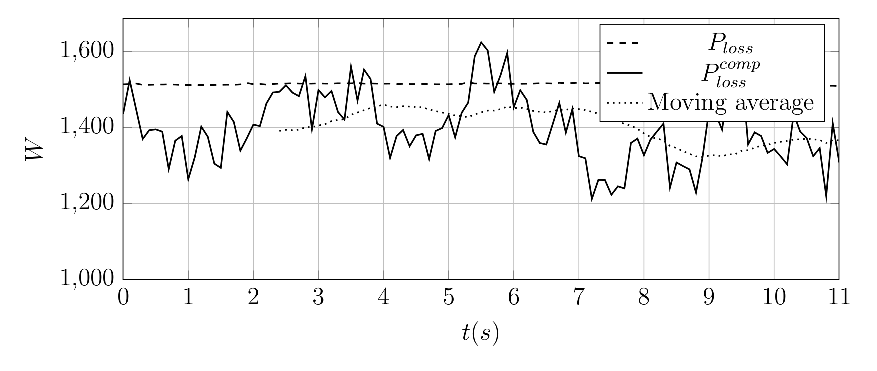
\includegraphics[width=0.95\textwidth]{Unblance_EPS_Pics/UnbalRedComp_JCP-figure6.eps}
%%             %\pgfplotsset{every tick label/.append style={font=\tiny},legend style={at={(1,1)},anchor=north east}}
%%             \pgfplotsset{every tick label/.append style={font=\normalsize}}
%%             \begin{tikzpicture}
%%             \begin{axis}[
%%             width=\textwidth,
%%             height=6cm,
%%             xlabel = {${t(s)}$},
%%             ylabel = {${W}$},
%%             grid=major,
%%             xmin=0,
%%             xmax=20,
%%             ymin=1000,
%%             ]
%%             \addplot[dashed,thick] table {netw_plot_nocont/P_loss.dat};
%%             \addplot[thick] table {netw_plot/P_loss.dat};
%%             \addplot[dotted,thick] table {netw_plot/P_loss_mean.dat};
%%             \legend{$P_{loss}$,$P^{comp}_{loss}$,Moving average}
%%             \end{axis}
%%             \end{tikzpicture}
%            \caption{Compensation control's loss reduction during zero energy balance operation on the modeled network, where $P_{loss}$ indicates the effective power losses and $P^{comp}_{loss}$ effective power losses during control of the network. As result the network losses reduced by mean $6.5\%$.}
%            \label{fig:compare_power}
%            \end{figure*}
%            The results show that despite of the negative cross effects of the intermediate voltage controller and the unbalance reduction controller it was possible to find the trade-off between the control goals of the different controllers (maintain zero energy balance for the inverter and decrease the unbalance on the network). The estimated loss reduction in the experimental setup is 6.5\%.
%            \begin{figure*}[ht]
%            \centering
%            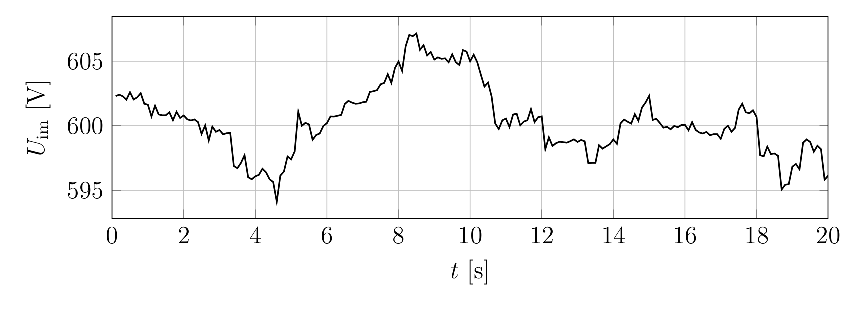
\includegraphics[width=0.95\textwidth]{Unblance_EPS_Pics/UnbalRedComp_JCP-figure7.eps}
%%                  %\pgfplotsset{every tick label/.append style={font=\tiny},legend style={at={(1,1)},anchor=north east}}
%%                 \pgfplotsset{every tick label/.append style={font=\normalsize}}
%%                 \begin{tikzpicture}
%%                 \begin{axis}[
%%                     width=\textwidth,
%%                     height=5cm,
%%                     xlabel = {$t$~[s]},
%%                     ylabel = {$U_{\textnormal{im}}$~[V]},
%%                     grid=major,
%%                     xmin=0,
%%                     xmax=20,
%%                     %ymin=0,
%%                     ]
%%                     \addplot[thick] table {netw_plot/U_inter.dat};
%%                     %\legend{\scriptsize$U_{intermediate}$}
%%                     \end{axis}
%%                  \end{tikzpicture}
%                 \caption{Intermediate puffer capacitance's voltage within boundaries ($600\pm10$\,V), during zero energy balance operation mode of the voltage unbalance compensation controller. $U_{\textnormal{im}}$ indicates intermediate the capacitance's voltage.}
%                 \label{fig:u_inter}
%                \end{figure*}
%
%        \paragraph[CO2 footprint]{CO$_2$ footprint}
%
%            The fact that this controller enables the reactive power reduction has a favourable consequence, i.e. the power loss or equivalently CO$_2$ emission and the carbon footprint can also be decreased. The estimated environmental effects of voltage asymmetry compensation can be calculated. Let us assume 3000\,kWh for the yearly electric energy consumption an average household and $9.173\%$ for the loss of the distribution network \cite{MVM2013}. With the controller the losses on the simulated network are reduced by 6.5\%. The calculation follows (\ref{eqn:co_emission})
%
%            \begin{equation}
%                \label{eqn:co_emission}
%                \begin{array}{rcl}
%                 P_{loss}&=&3000\,\textnormal{kWh}\cdot9.173\%\\
%                P^{comp}_{loss}&=&3000\,\textnormal{kWh}\cdot(9.173\cdot0.93)\%\\
%                 \Delta P_{loss}&=&P_{loss}-P^{comp}_{loss}\\
%                 \end{array}
%                \end{equation}
%
%            where $P_{loss}$ is the assumed network loss per household and $P^{comp}_{loss}$ is s the assumed network loss with unbalance compensation control and $\Delta P_{loss}$ is the saved energy. According to (\ref{eqn:co_emission}), unbalance compensation results in an energy savings of 19.26 kWh. Taking into account the proportion of power currently generated by fossil fuels (coal 17.3\,\%, gas 38.3\% \cite{MVM2013}, \cite{gorbe2012reduction}) and the rate of $\textnormal{CO}_2$ emission during electric energy production (1,000\,g/kWh from coal and 430\,g/kWh from gas), it can be concluded that voltage unbalance compensation could reduce $\textnormal{CO}_2$ emissions by 6504.9\,g a year, in an average household. %Note that this result reflect only the proof of concept, due the neglected power losses of the inverter and the artificial load of the network.
%
%
%\subsection{Conclusion}
%
%    The currently used measures of voltage unbalance has been extended in this work with a norm candidate. It is more demanding from the computational point of view but has an interesting feature namely it checks electrical asymmetry, i.e. the norm of a $\pm120$ degree  rotated version of the ideal three-phase phasor is zero in the geometrical sense.\\
%    The defined norm is applied as a cost function in the asymmetry reducing controller structure also presented in the paper. Simulations show that the geometrical based unbalance indicator can serve as a basis of further research. The suggested controller structure enables the residential users owning a grid synchronized domestic power plant to reduce voltage unbalance measurable at the connection point. The fundamental element of the system is a modified three phase inverter that is capable of the asymmetric injection of any current waveforms to the network. The optimization based control algorithm injects the available energy (as current waveform) in such a way, that the voltage unbalance decreases. This optimization problem is usually constrained by the available renewable energy supplied by the power plant.\\
%    The control structure has been tested on a low voltage network model in a dynamical simulation environment consisting of the models of the electrical grid, a domestic power plant,  asymmetrical inverter circuit, and different types of loads. Different simulation experiments has been run for each norm and for both the power constrained and unconstrained case. The preliminary results show that this structure can serve as a residential level voltage quality improvement method for the three phase low voltage network.


\newpage
\section{Notations used in the chapter}
		
		%\begin{longtable}{r|l}
  % after \\: \hline or \cline{col1-col2} \cline{col3-col4} ...
  \begin{scriptsize}
\begin{tabularx}{\textwidth}{r|X}



  

  %% A
%%$\textbf{A}$																& State matrix of a linear time invariant model\\
%%$\textbf{A}_x$              & Constraint state matrix\\
%%$\textbf{A}_u$              & Constraint input matrix\\
%%$\textbf{A}_f$              & Constraint state matrix at the end of the horizon\\
%%$\mathcal{A}$               & Set if indices in states where the constraints are active\\
%%$\mathcal{A}^N$               & Set if indices in states where the constraints are inactive\\
%%
%%
%%% B
%%$\textbf{B}$																& Input matrix of a linear time invariant model\\
%%$\textbf{b}_x$              & Constraint state coefficient\\
%%$\textbf{b}_u$              & Constraint input coefficient\\
%%$\textbf{b}_f$              & Constraint state coefficient at the end of the horizon\\
%%
%%% C
%$CVUF$  													& Complex Voltage Unbalance Factor\\
%%$\textbf{C}$																& Output matrix of a linear time invariant model\\
$C_{snub}$ 												& Capacitance to reduce switching loss and to damp out over-voltage\\
%%$C_D$															& Capacitance for filtering the output voltage of the VSR\\
%%$C_S$															& Input filter capacitance of the three phase alternating current in CSR\\
$\mathcal{C}$                           & APPS steps where $\Delta^t_i$ is reduced\\
%%$\mathcal{C}_{\mathcal{A}}$               & Critical region associated with the active constraints\\
%%
%%% D
$D_{1+},D_{2+}$										& CSI Higher diodes\\
$D_{1+},D_{2+}$										& CSI Lower diodes\\
$\mathcal{D}$                                       & APPS set of step directions\\
$d_i$												& APPS direction of active process\\
%%
%%% E
%%$\textbf{E}$                & Unified constraint state matrix \\
$\mathcal{E}$               & APPS set of external sucesses\\
%%
%%% F
%%$\textbf{F}$                & State coefficient matrix for calculating the optimal input \\
  $f(\textbf{x})$										& Multivariate function to minimize\\
%%
%%% G
$G$                               & Geometrical voltage unbalance indicator \\
%%$\textbf{G}$                & Unified constraint input matrix \\
%%$\mathcal{D}$               & Set of directions\\
%%$g$                         & Autonomous function where there are no inputs\\
%%$g_l$                       & Equality constraints of a Lagrange function\\
%%
%%% H
%%$\textbf{H}$                & Supplementary quadratic optimizer matrix\\
$h$                                                             & DC-DC transformer turn ratio\\
%%
%%% I

%$I_{0,1,2}$												& Zero positive and negarive sequence of current drop\\	
%%$I_D$															& Direct output current\\
$\mathcal{I}$               & APPS set if internal sucesses\\
%%$\mathcal{I}_c$               & Set if indices of constraints\\
%%$i_{abc}$                   & Generic three phase current\\
%%$i_i$															& Constant input inductor current\\
%%$i_o$															& Alternating output current\\
%%$i_{dq0}$                   & Three phase current converted to Park frame\\
%%$i_{\alpha\beta\gamma}$                   & Three phase current converted to Clarke frame\\
%%$\vec{i}$													& Rectifier input current\\
%%$\vec{i}_ref$											& Reference rectifier input current\\
%%
%%
%%% J
%%$J_0$                           & Cost (or value) function to optimize at the initial state\\
%%$J^*_0$            & Optimal cost value at the initial state\\
%%$\mathcal{J}$               & Set if indices of active constraints\\
%%
%%% K
%%$\textbf{K}$                & Controller gain\\
%%$\mathcal{K}$               & Set of states respective to constraints\\
%%$\mathcal{K}^*$               & Set of feasible states respective to constraints\\
%$k_v$  														& Magnitude of CVUF\\
%%$k$																& Time step on the horizon $N$ \\
%%
%%% L
$L_+,L_-$													& CSI current filter inductors\\
$L_a$															& DC-DC transformer leakage inductance\\
%%$L_S$															& Input filter inductance of the three phase alternating current in VSR\\
%%$L_D$															& Inductor for filtering the output current of the CSR (Choke)\\
%$LVUR$														& Voltage unbalance notation based on NEMA standard\\
%%
%%% M
%%$m$                             & Dimension of the input vector\\
%$m_{21}$                        & negative sequence factor, identical to $VUF$\\
%$m_{01}$                        & zero sequence factor\\
%%
%%
%%% N
%%$N$											& Defined horizon of MPC\\
%%$N_c,N_u,N_y$											& Defined control, input, and output horizon respectively\\
%%$n$                             & Dimension of the state vector\\
%%
%%% O
%%
%%% P
%%$\textbf{P}$                    & Terminal penalising weight matrix\\
$\mathcal{P}$                   & APPS set of processes\\
%%$\mathcal{P}^c$               & Set of all (input and state) constraints at time instance\\
%%$\mathcal{P}_p$             & Set of primary feasibility conditions\\
%%$\mathcal{P}_d$             & Set of dual feasibility conditions\\
$P_D$                           & DC-DC power transfer under idealized conditions\\
$P_{loss}$                        & Lost power per household due to network unbalance\\
  $P^{comp}_{loss}$                 & Assumed network loss with unbalance compensation control\\
  $\Delta P_{loss}$                 & Saved power with unbalance compensation control\\
  $\textbf{p}$                  & APPS search pattern\\
$p$                             & APPS process index\\


%$PVUR_{IEEE-141},PVUR_{IEEE-936}$	& Voltage unbalance notation based on IEEE-141, and IEEE-936 standard\\
%%$p$																& Process number\\
%%
%%% Q
%%$\textbf{Q}$                    & State penalising weight matrix\\
$\mathcal{Q}$                   & APPS set of sidestep indices\\
$q$																& Discrete time step\\
%%
%%% R

%%$\textbf{R}$                    & Input penalising weight matrix\\
%%
%%% S
$S_{1+},S_{2+}$										& CSI higher switches\\
$S_{1+},S_{2+}$										& CSI lower switches\\
%%$\textbf{S}$              & General state constraint coefficient\\
$\mathcal{S}$                   & APPS set of successful iterations\\
%%$\mathcal{S}^x$             & Set of all possible future state matrices stepping through the horizon\\
%%$\mathcal{S}^u$             & Set of all possible future input matrices stepping through the horizon\\
$s$                             & Dimension of the decision vector\\
%%
%%% T
$t_q$                             & Timestep of the algorithm at $q$\\
%%% U
%%$\textbf{U}^*_0$            & Optimal vector of future inputs starting from the initial state\\
$\mathcal{U}$              & APPS set of unsuccessful steps\\
%%$\mathcal{U}^u$             & Set of inputs not violating constraints\\
%%$\textbf{u}^*$            & Optimal vector of input\\
%%$\widehat{u}$				& Peak value of AC-side capacitor voltage\\
%%
%%% V
%%$V$                         & Lyapunov function\\
%$V_{ab},V_{bc},V_{ca}$  					& Line-to-line voltages\\
%$V_{avg_{line}}$  								& Average of line voltages\\	
%$V_{a},V_{b},V_{c}$  							& Phase-to-neutral voltages\\
$V_{an},V_{bn}$  									& Designated point's potential to ground \\
%$V_{avg_{phase}}$  								& Average of phase voltages\\
$V_i$															& Constant input voltage\\
$V_o$															& Alternating output voltage\\
%$V_{0},V_{p},V_{n}$  							& Zero, negative and positive sequence voltages based on symmetrical components theorem\\
$V_{D1},V_{D2}$ 									& Two end's voltage on the DC-DC converter\\
%%$V_d$															& Output voltage\\
%$\hat{V}$															& Voltage peak\\
%$\vec{V}_a, \vec{V}_b, \vec{V}_c,$										& Voltage vectors in the three phase phasor\\
$VUF$  														& Voltage Unbalance Factor\\
%$VUFactor,VU,VUR$                	& Non standardized voltage unbalance factor based on manufacturer standards\\
%%$v_{c_p}$													& AC-side capacitor voltage, where $p\in\{1,2,3\}$\\
$v_1,v_2$                         & DC-DC transformer voltages\\
%%$v_D$															& Output voltage before the choke inductor $L_D$\\
%%$v_{i,j}$													& Three phase phase-to-neutral voltage $i,j\in\{R,S,T\}$\\
%%$v_{N,RS}$												& Three phase line-to-line voltage of $R$ and $S$\\
%%
%%% W
%%$\textbf{w}$                & Unified constraint vector \\
%%
%%% X
%%$\mathcal{X}^x$             & Set of all possible future states stepping through the horizon\\
%%$\textbf{x}$											& State vector of a linear time invariant model\\
%%$\bar{\textbf{x}}$											& Minimum state value of the objective function\\
%%$\textbf{x}(0)$                 & Initial state\\
$\textbf{x}^{q}$                           & Local multivariate state at the $q^{th}$ timestep\\
$x_i^{best}$											& APPS best reached state, where $x_i^{best}$ is a minima\\
%%
%%% Y
%% $\textbf{Y}$ & Supplementary matrices\\
%%
%%% Z
%$Z$												& Symmetrical component mutual impedance\\
%%$\textbf{Z}^*$              & Set of optimizers leading to feasible states\\
%%$\textbf{z}$											& Optimizer of linear multi parametric problem\\
%%$\tilde{\textbf{z}}$        & Set of all future states and inputs over the horizon\\
%%
%%% Greek
$\alpha$													& Fortesque operator\\
%$\Delta U$													& Zero positive and negative sequence of voltage drop\\
$\Delta$													& APPS step length control parameter\\
$\Delta_i^{best}$											& APPS best reached step size\\
$\delta$                    & DC-DC modulation coefficient\\
$\Delta_q$                        & Step size at $q$\\
%$\theta$                    & Angular displacement of the voltage or current vector\\
%$\theta_v$  											& Angle of CVUF\\
$\lambda$                   & APPS system specific tunable parameter\\
$\theta$                    & APPS system specific tunable parameter\\
$\nu_i(q)$ 												& Time index for the completion of the function evaluation that produced the update at time step $q$ on process $i$\\
$\rho$																& APPS infinite sequence iterator\\
%%$\varphi_N$												& Angle of phase voltage\\
%$\upsilon$  											& Fortesque operator\\
$\tau_i(q)$												& Time index for initialization of the function evaluation, that produced the update at time $q$ on process $i$\\
$\omega$													& Angular velocity of output sinusoidal voltage or current\\
$\omega_i(q)$ 										& Generating process index for the update time at step $q$ on process $i$\\
$\bigtriangleup_{Ideal}$          & Triangle of Ideal voltage vectors\\
  $\bigtriangleup_{Real}$           & Triangle of real voltage vectors\\
  
\end{tabularx}
\end{scriptsize} 

% Explicit CSR
\chapter[Explicit predictive current control]{Explicit model predictive control of a current source buck-type rectifier}\label{BASIC:sec:MPC_CSR}

\section{Literature overview}\label{BASICCSR:sec:CSR_Literature}

%============ USAGE OF CURRENT SOURCE RECTIFIERS
Current source rectifiers (CSR) are widely used in front-end power electronic converter for the uncontrollable or controllable DC-bus in industrial and commercial applications. They have maintained their position through many applications, with uses such as medium-voltage high-power drives \cite{vajda2017limiting}, \cite{ghalem2010six} STATCOMs \cite{gupta2014two} and renewable systems \cite{chen2016single}, \cite{exposto2015predictive}. They have a plain and reliable circuit structure, which makes them attractive for simple control design. The CSRs are traditionally controlled by state feedback, or classic cascaded linear control loops such as PI controllers. These simple control applications are suitable for induction motor control \cite{chebre2011speed}, and other electromechanical actuators \cite{salloum2014robust}, and unusual topologies \cite{neukirchner2017voltage}. Also, worth mentioning of self-tuning variants of PI controllers \cite{tahri2012digital}.\\
%============ MODULATION OF CSR
 In the past, the modulation methods used were trapezoidal pulse width modulation techniques (TPWM), or application of pulse patterns calculated off-line for selective harmonic elimination (SHE). More recently, current space vector modulation (SVM) has been used for the synthesis of the transistor control signals \cite{gao2017model}. Even so, AC-side harmonic elimination could still be an issue at lower switching frequencies where LCL filtering (inductive-capacitive-inductive) would be advised \cite{han2010control}.\\
%============ TOPOLOGIES OF CSR
%In order to keep switching frequencies low and to minimize switching losses, new topologies and hybrid modulations are used, mixing TPWM and SHE depending on the grid frequency \cite{venkatraman2018multilevel}.\\
%============ BENEFITS OF CSR
    In terms of the amplitude of the grid and DC-link voltages, CSRs exhibit a step-down conversion. When used as DC voltage source, the rectifier can output a lower DC voltage without the need of a grid-side transformer, as is usually employed in voltage source rectifiers (VSR). Because of their current source behavior, CSRs can easily be paralleled and provide inherent short-circuit protection, representing an excellent potential in DC power supply applications \cite{feroura2017finite}, \cite{yan2015study}.\\		
%============ GENERAL POWER ELECTRIC CONTROL
    There are several control strategies in addition to classical PI control for applications in this domain. Self-adapting control methods are on the rise with more sophisticated algorithms in the field of fuzzy logic \cite{urmos2017application}. They are capable of handling increasingly more complicated models and systems with high dynamics and accuracy \cite{chatterjee2008augmented}, \cite{haidegger2012simulation}, and even without establishing and validating classical state-space models \cite{vrkalovic2018model}. The other filed is the sliding mode control, which can achieve good dynamic performance and handle non-linearity. Still, they might also introduce chattering, which can be very undesirable when applied to real-life systems like in \cite{regaya2014new} and \cite{szell2014mathematical}. Additionally in \cite{ahmed2014model} the validity of an MPC-based, digital pulse width modulation control strategy for single-phase voltage source rectifiers is discussed, further confirming the validity of this method in control systems.\\	
%============ PREDICTIVE POWER ELECTRIC CONTROL		
    In the linear domain implicit model predictive control (IMPC or MPC) is a fair solution due its effectiveness in power electronics because of its configurable cost function and such scalable nature \cite{kelemen2010constrained}, \cite{ahmed2014model}. In this field also finite-state solutions are present which can be considered also predictive control, where the modulation scheme’s defined states serve as optimization potential \cite{rivera2013predictive}, \cite{godlewska2015predictive}. As a further step adaptive application was established to tackle parameter estimation problems for better performance \cite{muthukumar2016adaptive}\\	
%============ EXPLICIT PREDICTIVE CONTROL
    Recently, beside implicit, finite-state, and adaptive predictive control, explicit model predictive control has emerged in the field of power electronics \cite{kutasi2010constrained}. Establishing the MPC cost function can range widely depending on the expected dynamics, degree of noise cancellation, and model complexity. Additionally, the current limitation can also be implemented introducing constraints in the modulation algorithm.\\	

\section{Three-phase buck-type rectifiers}\label{BASICCSR:sec:CSR}

Three-phase controlled rectifiers have a wide range of applications, from small rectifiers to large high-voltage direct-current transmission systems. They are used e.g. at electrochemical processes, many kinds of motor drives, traction equipment, controlled power supplies. In this thesis only force commuted rectifiers are examined, which are built with semiconductors (IGBTs in this case) with gate-turn-off capability. The gate-turn-off capability allows full control of the converter, because valves can be switched ON and OFF whenever is required. This allows the commutation of the valves, hundreds of times in one period that is not possible with line-commutated rectifiers, where IGBTs are switched ON and OFF only once a cycle. This has the following advantages:

\begin{itemize}
\item The current or voltage can be (pulse width) modulated, generating less harmonic contamination.
\item The power factor (ratio of the real and reactive power) can be controlled and even it can be made leading, signifies that the load is capacitive, as the load “supplies” reactive power.
\item They can be built as voltage-source or current-source based on the required application.
\item The reversal of power in switching rectifiers is by reversal of voltage at the DC link. This allows force commutated rectifiers can be implemented for both, reversal of voltage or reversal of current.
\end{itemize}

There are two ways to implement force commutated three phase rectifiers, as a current-source rectifier (Fig.\ref{BASICMPC:fig:CSR}), where power reversal is by DC voltage reversal, and as a voltage-source rectifier (Fig.\ref{BASICMPC:fig:VSR}), where power reversal is is solved by current reversal at the DC link.


\begin{figure}[h]
                \centering
                \begin{subfigure}[b]{0.9\textwidth}
                    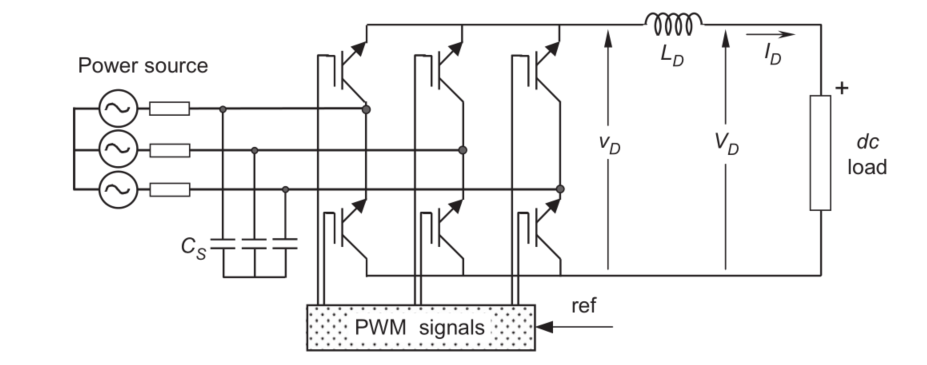
\includegraphics[width=\textwidth]{EMPC_PNG_Pics/BasicCurrentRectifiers.png}
                    \caption{\centering Current source rectifier with capacitive filtering and choke inductance.}
                    \label{BASICMPC:fig:CSR}
                \end{subfigure}
                ~ %add desired spacing between images, e. g. ~, \quad, \qquad, \hfill etc.
                  %(or a blank line to force the subfigure onto a new line)
                \begin{subfigure}[b]{0.9\textwidth}
                    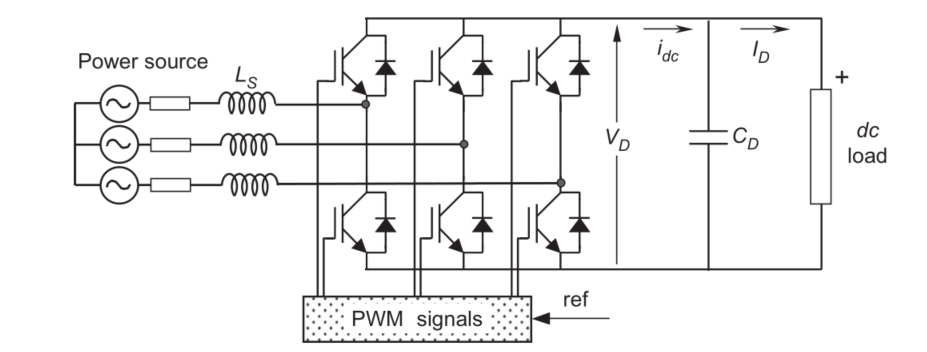
\includegraphics[width=\textwidth]{EMPC_PNG_Pics/BasicVoltageRectifiers.png}
                    \caption{\centering Voltage source rectifier with inductive filtering and DC voltage smoothing capacitance.}
                    \label{BASICMPC:fig:VSR}
                \end{subfigure}
                 %add desired spacing between images, e. g. ~, \quad, \qquad, \hfill etc.
                %(or a blank line to force the subfigure onto a new line)
                %\begin{subfigure}[b]{0.48\textwidth}
                    %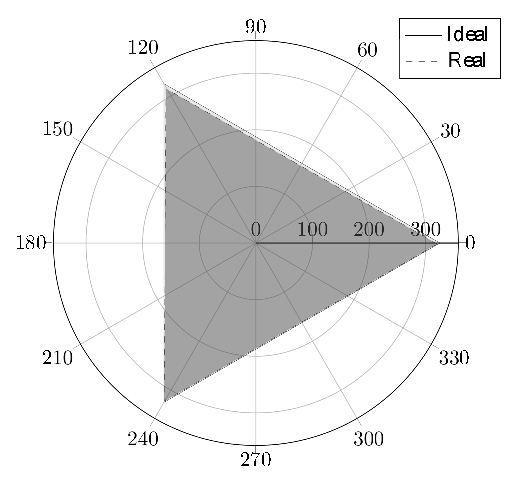
\includegraphics[width=\textwidth]{Unblance_EPS_Pics/EPS_images/square.eps}
                    %\caption{Low correlation with opposed amplitude deviation. The norm values are $G=9322$ and $TDV=0.5198$.}
                    %\label{fig:cases_C}
                %\end{subfigure}
                %~
                %\begin{subfigure}[b]{0.48\textwidth}
                    %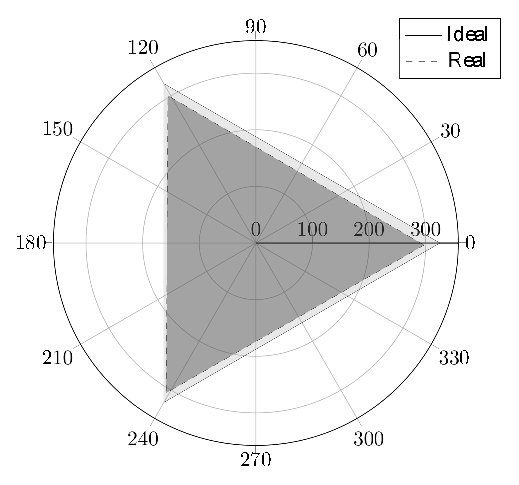
\includegraphics[width=\textwidth]{Unblance_EPS_Pics/EPS_images/circle.eps}
                    %\caption{\centering Low correlation with uniform voltage drop. The norm values are $G=6280$ and $TDV=0.156$.}
                    %\label{fig:cases_D}
                %\end{subfigure}


                \caption{Basic topologies of force commuted rectifiers.}
            \end{figure}

%\begin{figure}[!ht]
        %\centering
        %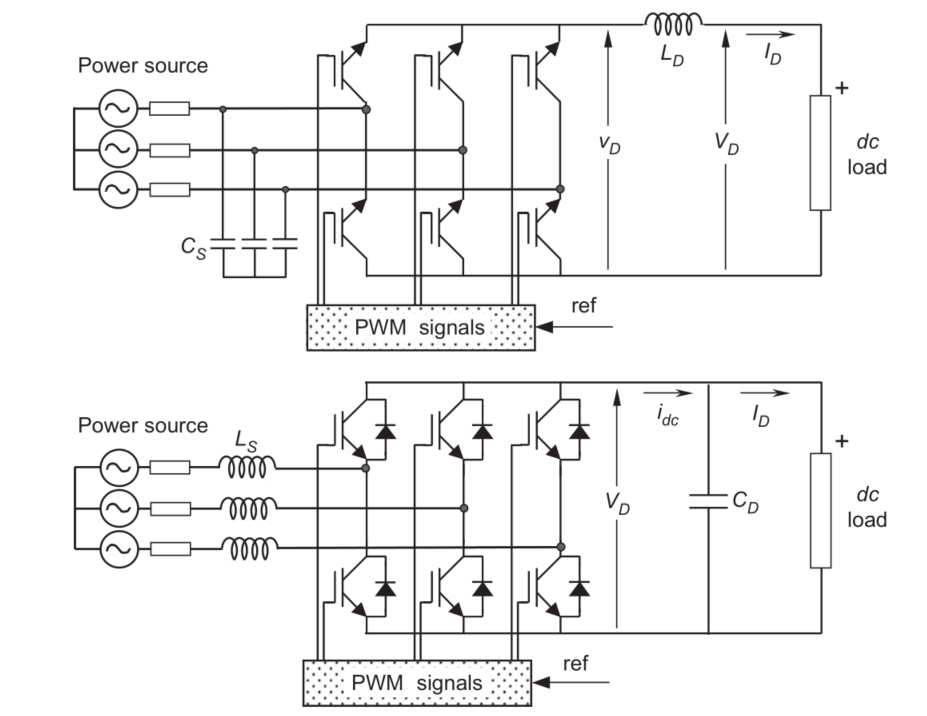
\includegraphics[width=0.9\textwidth]{EMPC_PNG_Pics/CurrentVoltageRectifiers.png}
        %\caption{Basic topologies of force commuted rectifiers.}
        %\label{BASICCSR:fig:topologies}
    %\end{figure}


As  general case be a front-end  converter power supply (e.g. lighting or telecommunications) shall be designed such that it should have approximately these general characteristics: sinusoidal main currents, unity power factor, high power density and simplicity of the power circuit structure. Two structures are most fitted for the task. First a boost-type input rectifier (e.g., Vienna rectifier, \cite{kolar1996design}), that typically features two $400$ V output voltages with a three-level isolated  DC-DC  converter  or  two  isolated  DC-DC  output  stage (see Fig. \ref{EMPC:fig:network} in Ch.5.). The second candidate is the buck-type  input  rectifier (or current source rectifier (CSR))  (conventionally  six-switch topologies as proposed in \cite{zargari1993current}, \cite{sato1993state}) with only one two-level isolated  DC-DC  converter  output  stage.  Also the  input  stage  can be realized as a three-switch topology with considerably  lower  system  complexity  as  compared  to  the boost-type structure. In particular, the number of utilized active and passive components is much lower. Furthermore, there is no middle-point that has to be stabilized, as this is the case for the boost-type structures, making control and active filter design less complex. Further system advantages are the potential of direct start-up and the implicit over current protection in case of an output short circuit. Therefore, these topologies of high interest for many safety critical applications as such future electric aircraft, or automotive applications or as power supplies for process technology \cite{nussbaumer2007comprehensive}.
The three-switch buck rectifier topology was first proposed in \cite{malesani1987three}. In \cite{itoh1989steady} and \cite{tooth2000effects}, aspects of the system modulation and control have been treated. The application of the topology used as an active filter is discussed in \cite{salo2005three}.  The addition of a DC-DC output boost-stage has been proposed in \cite{baumannnew} in order to maintain 400 V output voltage for a wide input voltage range and for the case of unbalanced mains as, e.g., the loss of one phase.

\myparagraph{Basic operation principles}\label{BASICCSR:sec:OperationPrinciple}

For the derivation of the relative on-times of the three buck transistors $S_i$ with the following assumptions are made for clarity and facilitation of calculations:
\begin{itemize}
	\item The AC-side filter capacitor voltages ($v_{c_p}$, where $p\in\{1,2,3\}$) at the input of the CSR are sinusoidal and in phase with the main harmonic component of voltage.
	
	\begin{equation}
        \begin{array}{rcl}
            v_{c_1}&=&\widehat{v}_c\cos(\omega t)\\
						v_{c_2}&=&\widehat{v}_c\cos(\omega t-2\pi/3)\\
						v_{c_3}&=&\widehat{v}_c\cos(\omega t+2\pi/3),\\
        \end{array}
        \label{BASICMPC:equ:phasorvect}
    \end{equation}
	where $\omega$ is the network voltage's angular velocity.
	
	\item The mains currents are assumed to be equal to the fundamental component of the rectifier input currents.
	\item The current in the DC output inductor $L_{D}$ is not affected by the high frequency ripple due to the switching operation.
\end{itemize}

 For achieving ohmic mains behavior also in case of unbalanced fundamental harmonics conditions the explained modulation method can still be utilized, however, additionally the control structure presented in \cite{baumann2005novel} has to be employed.\\
The waveforms of the phase and line-to-line mains voltages are divided into twelve sectors of $\frac{\pi}{6}$ rad wide shown in Fig.\ref{BASICCSR:fig:waves}. The following calculations are based on the analysis of the first sector which is characterized by the voltage harmonic phase relation. For the remaining sectors the calculations can be accomplished in an similar manner \cite{nussbaumer2007comprehensive}.

\begin{figure}[!ht]
        \centering
        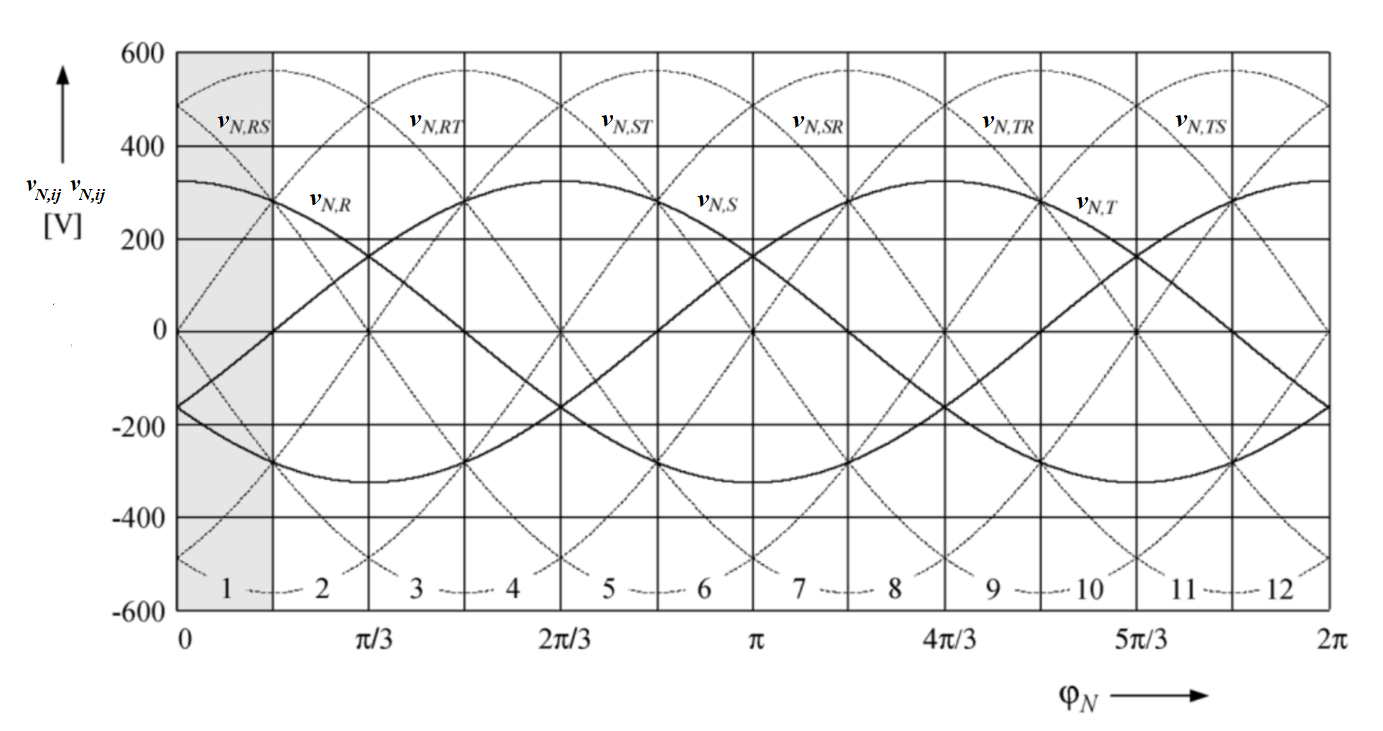
\includegraphics[width=\textwidth]{EMPC_PNG_Pics/Waves.png}
        \caption{Phase voltages $v_{i}$, where line-to-line voltages $v_{N,ij}=v_{N,i}-v_{N,j}$, $(i,j)\in\{R,S,T\}$ and sectors $1$ to $12$ being defined by the different relations of the instantaneous values of the mains phase voltages for $v = 400 V$}
        \label{BASICCSR:fig:waves}
    \end{figure}
		
		Accordingly, on AC side, if conditions are favorable, inductor current can appear in an instant of time either in two out
of three phases or in none. In this modulation technique, the switches in each converter leg can conduct only one at the time (aside from zero states, where both upper and lower switches are conducting). When the upper leg is conducting it is indicated by `$1$', when the lower  `$-1$' and when neither `$0$'. As such the choice whether upper or lower switch of the leg conducts current depends of the reference current vector's sector location.
According to the actual switch combination the DC link current shaped by the choke inductance, and distributed to two of the input phases or the freewheeling diode. With this, the input current space vectors can be calculated for each of the before-mentioned switching states. Generally the space vector of three-phase quantities (e.g., for the rectifier input current) are described as:

\begin{equation}
        \begin{array}{rcl}
            \vec{i}&=&\frac{2}{3}\left(\vec{i}_a+\vec{i}_be^{\frac{j\pi}{3}}+\vec{i}_bc^{\frac{4j\pi}{3}}\right).\\
        \end{array}
        \label{BASICCSR:eqn:currents_all}
    \end{equation}
		
		Based on \ref{BASICCSR:eqn:currents_all} the corresponding active space vectors in the first sector can be obtained as:
		
		\begin{equation}
        \begin{array}{rcl}
            \vec{i}_{(1,0,-1)}=\vec{i}_1&=&2i_{dc}e^{j\pi/6}/\sqrt{3}\\
						\vec{i}_{(0,1,-1)}=\vec{i}_2&=&2i_{dc}e^{j\pi/2}/\sqrt{3}\\
						\vec{i}_{(-1,1,0)}=\vec{i}_3&=&2i_{dc}e^{j5\pi/6}/\sqrt{3}\\
        \end{array}
        \label{BASICCSR:eqn:currents}
    \end{equation}
		
		The resulting discrete space vectors can be used to synthesize desired current
space vector $\vec{i}_{ref}$.

The modulation methods were evaluated in and chosen for this paper based on \cite{moussaoui2005open}, which ensures minimum switching-losses, minimum ripple values of the input capacitor voltages and of the output inductor current. According to this modulation, each pulse interval comprises two active states and a freewheeling state, arranged symmetrically about the middle of the pulse interval (see Table \ref{EMPC:tbl:sequence}). For more in depth functional description see section \ref{EMPC:sec:Modulation}.

\subsection{Coordinate transformations}

In section \ref{EMPC:sec:ModelofCSR} the three phase current source rectifier's (CSR) equations are converted to different coordinate spaces.

\subsubsection{Clarke transformation}\label{BASICCSR:sec:Clarke}

In electrical engineering, Clarke transformation is a mathematical transformation employed to simplify the analysis of three-phase circuits. Conceptually it is similar to the Park transformation. One very useful application is the generation of the reference signal used for space vector modulation control of three-phase inverters. The transformation follows:

\begin{equation}
        \begin{array}{rcl}
            \textbf{i}_{\alpha\beta\gamma}(t)&=&T_{Clarke}\textbf{i}_{abc}(t)
            \begin{bmatrix}
            1& -\frac{1}{2}& -\frac{1}{2}\\
            0& \frac{\sqrt{3}}{2}& -\frac{\sqrt{3}}{2}\\
            \frac{1}{2}& \frac{1}{2}& \frac{1}{2}\\
            \end{bmatrix}
            \begin{bmatrix}
            i_a(t)\\
            i_b(t)\\
            i_c(t)\\
            \end{bmatrix},
        \end{array}
        \label{BASICCSR:eqn:Clarke}
    \end{equation}

    where $\textbf{i}_{abc}$ is the generic three phase current sequence, and $\textbf{i}_{\alpha\beta\gamma}$ is given by the transformation.

    \subsubsection{Park transformation}\label{BASICCSR:sec:Park}

The Park transformation is a tensor that rotates the reference frame of a three-element vector or a three-by-three element matrix in an effort to simplify analysis. The transform can be used to rotate the reference frames of AC waveforms such that they become DC signals. Simplified calculations can then be carried out on these dc quantities before performing the inverse transform to recover the actual three-phase ac results. As an example, the Park transform is often used in order to simplify the analysis of three-phase synchronous machines or to simplify calculations for the control of three-phase inverters. In analysis of three-phase synchronous machines the transformation transfers three-phase stator and rotor quantities into a single rotating reference frame to eliminate the effect of time-varying inductances. The transformation follows:


\begin{equation}
        \begin{array}{rcl}
            \textbf{i}_{dq0}(t)&=&T_{Park}\textbf{i}_{abc}(t)
            \sqrt{\frac{2}{3}}\begin{bmatrix}
            \cos(\theta)& \cos(\theta-\frac{2\pi}{3})& \cos(\theta+\frac{2\pi}{3})\\
            -\sin(\theta)& -\sin(\theta-\frac{2\pi}{3})& -\sin(\theta+\frac{2\pi}{3})\\
            \frac{\sqrt{2}}{2}& \frac{\sqrt{2}}{2}& \frac{\sqrt{2}}{2}\\
            \end{bmatrix}
            \begin{bmatrix}
            i_a(t)\\
            i_b(t)\\
            i_c(t)\\
            \end{bmatrix},
        \end{array}
        \label{BASICCSR:eqn:Park}
    \end{equation}

    where $\theta$ is instantaneous angular position of an arbitrary frequency.

\section{Model based predictive control}

\subsection{Quadratic optimization and predictive control}\label{BASICCSR:sec:MPC}

Philosophically MPC reflects human behavior whereby we select control actions which we think will lead to the best predicted outcome (or output) over some limited horizon. To make this selection we use an internal model of the process in question, and constantly update our decisions as new observations become available. Hence a predictive control law has the following components:
\begin{itemize}
\item The control law depends on predicted behavior.
\item The output predictions are computed using a process model.
\item The current input is determined by optimizing some measure of predicted performance.
\item The receding horizon: the control input is updated at every sampling instant.
\end{itemize}

%\myparagraph{Model predictive control}\label{BASICCSR:sec:MPCOverview}
Most control laws, say PID (proportional, integral and derivative) control, does not explicitly consider the future implication of current control actions. To some extent this is only accounted by the expected closed-loop dynamics. MPC on the other hand
implicitly (or explicitly) computes the predicted behavior over some horizon. One can therefore restrict the choice of the proposed input trajectories to those that do not lead to difficulties in the future.\\
In order to predict the future behavior of a process, we must have a model of how the process behaves. In particular, this model must show the dependence of the output on the current measured variable and the current/future inputs. This does not have to be linear (e.g. transfer function, state-space) and in fact can be just about anything. A precise model is not always required to get tight control, because the decisions are updated regularly. This will deal with some model uncertainty in a fairly fast time scale. The decision on the best control is thus continually updated using information from this comparison \cite{rossiter2017model}.\\
This way, model based predictive control methods are optimal regulators, with a defined cost function on a defined and encompassed prediction horizon with restrictions \cite{kwon2006receding}, \cite{baotic2005optimal}, \cite{herceg2009real}, \cite{grancharova2005survey}. The control signal is calculated over a defined horizon, but from the sequence of applicable control signals only the first one is used in the next sample. This procedure is repeated according to the principle of the moving horizon, using new iterations, as such provides the reaction in each sample. The method was developed for systems with physical restrictions, in the first stage for the control of chemical processes in the oil industry, then it was applied to various rapid processes from automotive or power electronics industry \cite{antoniewicz2009predictive} , \cite{geyer2005low}. By default the optimization problem can be solved, for each sample, or explicitly using the multi-parameter programming techniques (mp-LP, mp-QP).% presented in \textbf{[N-ANNEX 1]-(Needed?)}, over a well-defined parameter space.

	\myparagraph{Linear quadratic optimal control}\label{BASICCSR:sec:LQR}

In practice most MPC algorithms use linear models because the dependence of the predictions on future control choices is then linear and this facilitates optimization as well as off-line analysis of expected closed-loop behavior. However, nonlinear models can be used where the implied computational burden is not a problem and linear approximations are not accurate enough. It is also important to note here the comment fit for purpose. In predictive control, the model is used solely to compute system output predictions, so the model is fit for purpose if it gives accurate enough predictions. The effort and detail put into modeling stage should reflect this.	Let the us assume that the system is linear and time-invariant (LTI):
	
	    \begin{equation}
        \begin{array}{rcl}
            \textbf{x}(q+1)&=&\textbf{Ax}(q)+\textbf{Bu}(q),\\
						%\textbf{y}(q)&=&\textbf{Cx}(q)
        \end{array}
        \label{BASICMPC:equ:basic_LTI}
    \end{equation}

    where $\textbf{x}(q)\in\mathbb{R}^n$ and $\textbf{u}(q)\in\mathbb{R}^m$ are the state and input vectors respectively. We define a quadratic cost function over a finite horizon of $N$ steps:

\begin{equation}
        \begin{array}{rcl}
				%&&\norm{asd}
         J_0(\textbf{U}_0,x(0))&=&\textbf{x}'_N\textbf{P}\textbf{x}_N+\sum^{N-1}_{k=0}\textbf{x}'_k\textbf{Q}\textbf{x}_k+\textbf{u}'_k\textbf{R}\textbf{u}_k\\
        \end{array}
        \label{BASICMPC:equ:cost_function_Euclidian}
    \end{equation}

    where $U_0=[\textbf{u}'_0,\dots,\textbf{u}'_{N-1}]\in\mathbb{R}^s$, $s=m\cdot N$ is the decision vector (with $m$ dimensional input vector) constraining all future inputs, also $\textbf{P}=\textbf{P}'\succeq 0$, $\textbf{Q}=\textbf{Q}'\succeq 0$, $\textbf{R}=\textbf{R}'\succeq 0$, and $\textbf{x}_k$ denotes the state vector at time $k$ obtained form $\textbf{x}_0=\textbf{x}(0)$. We also apply the system model based on \ref{BASICMPC:equ:basic_LTI}:

    \begin{equation}
        \begin{array}{rcl}
            \textbf{x}_{k+1}&=&\textbf{Ax}_k+\textbf{Bu}_k,\\
						%\textbf{y}(q)&=&\textbf{Cx}(q)
        \end{array}
        \label{BASICMPC:equ:basic_horizon model}
    \end{equation}

   From the above a finite optimal control problem can be considered:

   \begin{equation}
        \begin{array}{rcl}
				%&&\norm{asd}
         J^*_0(\textbf{x}(0))&=&\min_{\textbf{U}_0}J_0(\textbf{U}_0,x(0))\\
         &\textnormal{subj. to}&\textbf{x}_{k+1}=\textbf{Ax}_k+\textbf{Bu}_k\\
         &&\textbf{x}_0=\textbf{x}(0)\\
         &&k=0,1,\dots,N-1
        \end{array}
        \label{BASICMPC:equ:optimal_control_problem_Euclidian}
    \end{equation}


    The first step is to write the equality constraints to express all future states and inputs from the initial state $\textbf{x}_0$ until the and of horizon $N$:

    \begin{equation}
        \begin{array}{rcl}
        \underbrace{
        \begin{bmatrix}
        \textbf{x}(0)\\
        \textbf{x}_1\\
        \vdots\\
        \vdots\\
        \textbf{x}_N\\
        \end{bmatrix}}_{\mathcal{X}^x}
        &=&
        \underbrace{
        \begin{bmatrix}
        \textbf{I}_0\\
        \textbf{A}_1\\
        \vdots\\
        \vdots\\
        \textbf{A}^N\\
        \end{bmatrix}}_{\mathcal{S}^x}\textbf{x}(0)+
        \underbrace{
        \begin{bmatrix}
        0& \dots& \dots& 0\\
        \textbf{B}& 0& \dots& 0\\
        \textbf{AB}& \ddots& \ddots& \vdots\\
        \vdots& \ddots& \ddots& \vdots\\
        \textbf{A}^{N-1}\textbf{B}& \ddots& \ddots& \textbf{B}\\
        \end{bmatrix}}_{\mathcal{S}^u}
        \begin{bmatrix}
        \textbf{u}_0\\
        \vdots\\
        \vdots\\
        \textbf{u}_N\\
        \end{bmatrix}.

		\end{array}
        \label{BASICMPC:equ:batch_allstates}
    \end{equation}

    %For the easier notation it is asmued that $\mathcal{X^x}={\textbf{x}(0),\textbf{x}_1,\dots,\textbf{x}_N}$, $\mathcal{S^x}={\textbf{I},\textbf{A},\dots,\textbf{x}_N}$ $ \underbrace{(x + 2)^3}_{\text{text 1}}$
    Here all future states are explicit functions of the state $\textbf{x}(0)$ and the future inputs of $\textbf{u}_0,\textbf{u}_1\cdot$ only. By defining appropriate quantities, we can rewrite \ref{BASICMPC:equ:batch_allstates} in a compact form:

    \begin{equation}
        \begin{array}{rcl}
        \mathcal{X}^x&=&\mathcal{S}^x(0)+\mathcal{S}^u\textbf{U}_0.\\
		\end{array}
        \label{BASICMPC:equ:batch_allstates_compact}
    \end{equation}

    Using the same notation the object function can be rewritten as:

    \begin{equation}
        \begin{array}{rcl}
        J(\textbf{x}_0,\textbf{U}_0)&=&\mathcal{X}'\bar{\textbf{Q}}\mathcal{X}+\textbf{U}_0\bar{\textbf{Q}}\textbf{U}'_0,\\
		\end{array}
        \label{BASICMPC:equ:batch_object}
    \end{equation}

    where $\bar{\textbf{Q}}=diag\{\textbf{Q},\dots,\textbf{Q},\textbf{P}\}$, and $\bar{\textbf{R}}=diag\{\textbf{R},\dots,\textbf{R}\}$. Substituting \ref{BASICMPC:equ:batch_allstates_compact} into the objective function \ref{BASICMPC:equ:batch_object} yields:

    \begin{equation}
        \begin{array}{rcl}
        J(\textbf{x}_0,\textbf{U}_0)&=&(\mathcal{S}^x(0)+\mathcal{S}^u\textbf{U}_0)'\bar{\textbf{Q}}(\mathcal{S}^x(0)+\mathcal{S}^u\textbf{U}_0)+\textbf{U}_0'\bar{\textbf{R}}\textbf{U}_0\\
        &=&\textbf{U}'_0\underbrace{(\mathcal{S}^{u'}\bar{\textbf{Q}}\mathcal{S}^u+\bar{\textbf{R}})}_{\textbf{H}}\textbf{U}_0+ \\
        &+&2\textbf{x}'(0)\underbrace{(\mathcal{S}^{x'}\bar{\textbf{Q}}\mathcal{S}^u)}_{\textbf{F}}\textbf{U}_0+\\
        &+&\textbf{x}'(0)\underbrace{(\mathcal{S}^{x'}\bar{\textbf{Q}}\mathcal{S}^x)}_{\textbf{Y}}\textbf{x}(0)\\
        &=&\textbf{U}'_0\textbf{H}\textbf{U}_0+2\textbf{x}'(0)\textbf{F}\textbf{U}_0+\textbf{x}'(0)\textbf{Y}\textbf{x}(0).
		\end{array}
        \label{BASICMPC:equ:batch_simplfy}
    \end{equation}

    Because $\bar{\textbf{R}}\succ 0$, and $\textbf{H}\succ 0$, thus $J(\textbf{x}_0,\textbf{U}_0)$ is a positive definite quadratic function of $\textbf{U}_0$, therefore its minimum can be found by computing its gradient and setting it to zero, which yields the optimal vector of future inputs:
%
    \begin{equation}
        \begin{array}{rcl}
        \textbf{U}^*_0(\textbf{x}(0))&=&-\textbf{H}^{-1}\textbf{F}'x(0)\\
        &=&-(\mathcal{S}^{u'}\bar{\textbf{Q}}\mathcal{S}^{u}+\bar{\textbf{R}})^{-1}\mathcal{S}^{u'}\bar{\textbf{Q}}\mathcal{S}^{x}\textbf{x}(0).
		\end{array}
        \label{BASICMPC:equ:batch_optimal_solution}
    \end{equation}

    With \ref{BASICMPC:equ:batch_optimal_solution} applied and calculated $\textbf{U}_0$ the cost is the optimal following:

    \begin{equation}
        \begin{array}{rcl}
        \textbf{J}^*_0(\textbf{x}(0))&=&-\textbf{x}(0)'\textbf{F}\textbf{H}^{-1}F'x(0)\\
        &=&\textbf{x}(0)'\left[ \mathcal{S}^{x'}\bar{\textbf{Q}}\mathcal{S}^{x} - \mathcal{S}^{x'}\bar{\textbf{Q}}\mathcal{S}^{u}
        (\mathcal{S}^{u'}\bar{\textbf{Q}}\mathcal{S}^{u}+\bar{\textbf{R}})^{-1}\mathcal{S}^{u'}\bar{\textbf{Q}}\mathcal{S}^{x}  \right]\textbf{x}(0).
		\end{array}
        \label{BASICMPC:equ:batch_optimal_cost}
    \end{equation}

    Note that the optimal vector of future inputs $\textbf{U}^*_0(\textbf{x}(0))$ is a linear function of \ref{BASICMPC:equ:batch_optimal_solution} of the initial state $\textbf{x}(0)$ and the optimal cost $J^*_0(x(0))$ is a quadratic function \ref{BASICMPC:equ:batch_optimal_cost} of the initial state $\textbf{x}(0)$.\\
    Alternatively the formulation can be done in a recursive manner. The optimal cost can be defined as $J^*_j(\textbf{x}_j)$ fot the $j^{th}$ for the $N-j$ step problem starting from state $\textbf{x}_j$ as:

    \begin{equation}
        \begin{array}{rcl}
				%&&\norm{asd}
         J^*_j(\textbf{x}_j)&=&\min_{\textbf{u}_j,\dots,\textbf{u}_{N-1}}\textbf{x}'_N\textbf{P}\textbf{x}_N+\sum^{N-1}_{k=0}\textbf{x}'_k\textbf{Q}\textbf{x}_k+\textbf{u}'_k\textbf{R}\textbf{u}_k.\\
        \end{array}
        \label{BASICMPC:equ:cost_function_Euclidian_recursive}
    \end{equation}

    The optimal "one step cost to go" can be obtained as:

     \begin{equation}
        \begin{array}{rcl}
				%&&\norm{asd}
         J^*_{N-1}(\textbf{x}_{N-1})&=&\min_{\textbf{u}_{N-1}}\textbf{x}'_N\textbf{P}_N\textbf{x}_N+\textbf{x}'_{N-1}\textbf{Q}\textbf{x}_{N-1}+\textbf{u}'_{N-1}\textbf{R}\textbf{u}_{N-1}.\\
          &\textnormal{subj. to}&\textbf{x}_N=\textbf{Ax}_{N-1}+\textbf{Bu}_{N-1}\\
          &&\textbf{P}_N=\textbf{P},\\
        \end{array}
        \label{BASICMPC:equ:cost_function_Euclidian_recursive_onestep}
    \end{equation}

    where $J^*_{N-1}(\textbf{x}_{N-1})$ is a positive quadratic function of the decision variable $\textbf{u}_{N-1}$. Writing \ref{BASICMPC:equ:cost_function_Euclidian_recursive_onestep} as the objective function:

    \begin{equation}
        \begin{array}{rcl}
				%&&\norm{asd}
         J^*_{N-1}(\textbf{x}_{N-1})&=&\min_{\textbf{u}_{N-1}}\{\textbf{x}'_{N-1}(\textbf{A}'\textbf{P}_N\textbf{A}+\textbf{Q})\textbf{x}_{N-1}+\\
         &+&2\textbf{x}'_{N-1}\textbf{A}'\textbf{P}_N\textbf{B}\textbf{u}_{N-1}+\\
         &+&\textbf{u}'_{N-1}(\textbf{B}'\textbf{P}_N\textbf{B}+\textbf{R})\textbf{x}_{N-1}\}.\\
        \end{array}
        \label{BASICMPC:equ:cost_function_Euclidian_recursive_substituted}
    \end{equation}

    The optimal input can be found by setting the gradient to zero:

    \begin{equation}
        \begin{array}{rcl}
        \textbf{u}^*_{N-1}=\underbrace{-(\textbf{B}'\textbf{P}_N\textbf{B}+\textbf{R})^{-1}\textbf{B}'\textbf{P}_N\textbf{A}}_{\textbf{F}_{N-1}}\textbf{x}_{N-1},\\
        \end{array}
        \label{BASICMPC:equ:cost_function_Euclidian_recursive_optimum}
    \end{equation}

    and the optimal one step optimal cost:

    \begin{equation}
        \begin{array}{rcl}
        J^*_{N-1}(\textbf{x}_{N-1})&=&\textbf{x}'_{N-1}\textbf{P}_{N-1}\textbf{x}_{N-1},\\
        \end{array}
        \label{BASICMPC:equ:cost_function_Euclidian_recursive_stepback}
    \end{equation}

    where $\textbf{P}_{N-1}$ can be defined recursively as:

    \begin{equation}
        \begin{array}{rcl}
        \textbf{P}_{N-1}=\textbf{A}'\textbf{P}_N\textbf{A}+\textbf{Q}-\textbf{A}'\textbf{P}_N\textbf{B}(\textbf{B}'\textbf{P}_N\textbf{B}+\textbf{R})^{-1}\textbf{B}'\textbf{P}_N\textbf{A}.\\
        \end{array}
        \label{BASICMPC:equ:cost_function_Euclidian_recursive_P}
    \end{equation}

    The next stage is to write down the "two step" problem based on \ref{BASICMPC:equ:cost_function_Euclidian_recursive_onestep}:

    \begin{equation}
        \begin{array}{rcl}
				%&&\norm{asd}
         J^*_{N-2}(\textbf{x}_{N-2})&=&\min_{\textbf{u}_{N-2}}\textbf{x}'_{N-1}\textbf{P}_{N-1}\textbf{x}_{N-1}+\textbf{x}'_{N-2}\textbf{Q}\textbf{x}_{N-2}+\textbf{u}'_{N-2}\textbf{R}\textbf{u}_{N-2}.\\
          &\textnormal{subj. to}&\textbf{x}_{N-1}=\textbf{Ax}_{N-2}+\textbf{Bu}_{N-2}\\
          %&&\textbf{P}_N=\textbf{P},\\
        \end{array}
        \label{BASICMPC:equ:cost_function_Euclidian_recursive_twostep}
    \end{equation}

    We since \ref{BASICMPC:equ:cost_function_Euclidian_recursive_twostep} has the same form as \ref{BASICMPC:equ:cost_function_Euclidian_recursive_onestep} we can apply the same solution seen at \ref{BASICMPC:equ:cost_function_Euclidian_recursive_optimum}:

    \begin{equation}
        \begin{array}{rcl}
        \textbf{u}^*_{N-2}=\underbrace{-(\textbf{B}'\textbf{P}_{N-1}\textbf{B}+\textbf{R})^{-1}\textbf{B}'\textbf{P}_{N-1}\textbf{A}}_{\textbf{F}_{N-2}}\textbf{x}_{N-2},\\
        \end{array}
        \label{BASICMPC:equ:cost_function_Euclidian_recursive_optimum_twostep}
    \end{equation}

    where the "two step" cost:

    \begin{equation}
        \begin{array}{rcl}
        J^*_{N-2}(\textbf{x}_{N-2})&=&\textbf{x}'_{N-2}\textbf{P}_{N-2}\textbf{x}_{N-2},\\
        \end{array}
        \label{BASICMPC:equ:cost_function_Euclidian_recursive_twostepback}
    \end{equation}

    where $\textbf{P}_{N-2}$ can be defined recursively as:

    \begin{equation}
        \begin{array}{rcl}
        \textbf{P}_{N-2}=\textbf{A}'\textbf{P}_{N-1}\textbf{A}+\textbf{Q}-\textbf{A}'\textbf{P}_{N-1}\textbf{B}(\textbf{B}'\textbf{P}_{N-1}\textbf{B}+\textbf{R})^{-1}\textbf{B}'\textbf{P}_{N-1}\textbf{A}.\\
        \end{array}
        \label{BASICMPC:equ:cost_function_Euclidian_recursive_twoP}
    \end{equation}

    Continuing in this manner at some arbitrary time $k$ the optimal control action is:

    \begin{equation}
        \begin{array}{rcl}
        \textbf{u}^*(k)=\underbrace{-(\textbf{B}'\textbf{P}_{k+1}\textbf{B}+\textbf{R})^{-1}\textbf{B}'\textbf{P}_{k+1}\textbf{A}}_{\textbf{F}_{k}}\textbf{x}_{k},\\
        \end{array}
        \label{BASICMPC:equ:cost_function_Euclidian_recursive_optimum_anystep}
    \end{equation}

    where $k=0,1,\dots,N-1$ and:

    \begin{equation}
        \begin{array}{rcl}
        \textbf{P}_{k}=\textbf{A}'\textbf{P}_{k+1}\textbf{A}+\textbf{Q}-\textbf{A}'\textbf{P}_{k+1}\textbf{B}(\textbf{B}'\textbf{P}_{k+1}\textbf{B}+\textbf{R})^{-1}\textbf{B}'\textbf{P}_{k+1}\textbf{A}.\\
        \end{array}
        \label{BASICMPC:equ:cost_function_Euclidian_recursive_twoP}
    \end{equation}

    and the optimal starting cost starting from the measured state:

     \begin{equation}
        \begin{array}{rcl}
        J^*_{k}(\textbf{x}(k))&=&\textbf{x}'(k)\textbf{P}_{k}\textbf{x}(k).\\
        \end{array}
        \label{BASICMPC:equ:cost_function_Euclidian_recursive_anystepback}
    \end{equation}

    Equation \ref{BASICMPC:equ:cost_function_Euclidian_recursive_twoP} is called the discrete Ricatti equation \cite{borrelli2017predictive}, or Ricatti difference equation, which is initialised with $\textbf{P}_n=\textbf{P}$ and solves backwards. It is worth noting that from \ref{BASICMPC:equ:cost_function_Euclidian_recursive_optimum_anystep} the optimal control action $\textbf{u}^*(k)$ is obtained in the form of feedback law as linear function of the measured state $\textbf{x}(k)$ at time instance $k$, and the optimal cost is \ref{BASICMPC:equ:cost_function_Euclidian_recursive_anystepback}.

	
	\myparagraph{Constrained optimal control}\label{BASICCSR:sec:OptimalControl}
	
	In constrained optimal control for any input action with a given initial state the control action can be computed with quadratic programming but with respect to pre described constraints. As displayed, the linear quadratic approach requires a numerical definition so that a precise calculation can be made, that is, which optimal input trajectory gives the lowest numerical value to the cost. The main requirement is that the cost depends on the batch or recursive input sequence and that low values of cost imply good closed-loop performance good being defined for the process. Of course the choice of the cost affects the complexity of the implied optimization and this is also a consideration.\\
With considering an LTI system such as \ref{BASICMPC:equ:basic_LTI}, let us assume that it is subject to constraints:

\begin{equation}
        \begin{array}{rcl}
            \textbf{x}(q)\in\mathcal{X}^x,&\textnormal{ }\textbf{u}(q)\in\mathcal{U}^u,&\textnormal{ }\forall t\geq0,\\
						%\textbf{y}(q)&=&\textbf{Cx}(q)
        \end{array}
        \label{BASICMPC:equ:basic_LTI_constrained}
    \end{equation}

    where the set of inputs $\mathcal{U}^u\subseteq\mathbb{R}^m$ and states $\mathcal{X}^x\subseteq\mathbb{R}^n$ are polyhedra. when Eucledian norm is used with the cost as \ref{BASICMPC:equ:cost_function_Euclidian} with $\textbf{P}\succeq0$, $\textbf{Q}\succeq0$, and $\textbf{R}\succ0$ we define the constrained optimal control problem as:

    \begin{equation}
        \begin{array}{rcl}
            J^*_0(\textbf{x}(0))&=&\min_{\textbf{U}_0}J_0(\textbf{x}(0),\textbf{U}_0)\\
            &\textnormal{subj. to}&\textbf{x}_{k+1}=\textbf{Ax}_{k}+\textbf{Bu}_{k},k=0,1,\dots,N-1\\
            &&\textbf{x}_N\in\mathcal{X}_f,\textbf{x}_k\in\mathcal{X}^x,\textbf{u}_k\in\mathcal{U}^u\\
            &&\textbf{x}_0=\textbf{x}(0),
        \end{array}
        \label{BASICMPC:equ:constrained_optimal_control_problem}
    \end{equation}

    where $\textbf{x}_N\subseteq\mathbb{R}^n$ is the terminal polyhedral region, and $\textbf{U}_0=[\textbf{u}'_0,\dots,\textbf{u}'_{N-1}]'\in\mathbb{R}^s$ with $s=m\cdot N$ is the optimization vector. We denote $\mathcal{X}_0\subset\mathcal{X}^x$ as the set of initial states $\textbf{x}(0)$ for which the optimal control problem is feasible such as:

    \begin{equation}
        \begin{array}{rcl}
            \mathcal{X}_0&=&\{
            \textbf{x}_0\in\mathbb{R}^n:\exists\textbf{U}_0,\\
            &&s.t.:\textbf{x}_k\in\mathcal{X}^x,\textbf{u}_k\in\mathcal{U}^u,\textbf{x}_N\in\mathcal{X}_f,\\
            &&where\,\textbf{x}_{k+1}=\textbf{Ax}_{k}+\textbf{Bu}_{k},k=0,\dots,N-1
            \}.\\
        \end{array}
        \label{BASICMPC:equ:constrained_initial_set}
    \end{equation}

    We denote $\mathcal{X}_i$ as the set of states $\textbf{x}_i$ at time $i=0,1,\dots,N$ which is feasible for \ref{BASICMPC:equ:constrained_optimal_control_problem}. The sets $\mathcal{X}_i$ are independent of the cost function as long as it guaranties the exsistence of a minima and the algorithm used to compute the solution. There are also ways to define an compute $\mathcal{X}_i$. With the batch approach is as follows:

    \begin{equation}
        \begin{array}{rcl}
            \mathcal{X}_i&=&\{
            \textbf{x}_i\in\mathbb{R}^n:\exists\textbf{U}_i,\\
            &&s.t.:\textbf{x}_k\in\mathcal{X}^x,\textbf{u}_k\in\mathcal{U}^u,\textbf{x}_N\in\mathcal{X}_f,\\
            &&where\,\textbf{x}_{k+1}=\textbf{Ax}_{k}+\textbf{Bu}_{k},k=0,\dots,N-1
            \}.\\
        \end{array}
        \label{BASICMPC:equ:constrained_feasible_set}
    \end{equation}

    This definition requires, that for any initial $\textbf{x}_i\in\mathcal{X}_i$ state there exsists a feasible $\textbf{U}_i=[\textbf{u}_i,\dots,\textbf{u}_{N-1}]$ which keeps the state evolution in the feasible set $\mathcal{X}^x$ at future time instants $k$ and forces $\textbf{x}_N$ into $\mathcal{X}_f$ at $k=N$.\\
    Next we show how to compute $\mathcal{X}_i$ for $i=0,\dots,N-1$. It is stated that the state $\mathcal{X}^x$, $\mathcal{X}_f$ and input $\mathcal{U}^u$ sets are $\mathcal{H}$-polyhedra \cite{borrelli2017predictive}, and $\textbf{A}_x\leq\textbf{x}\textbf{b}_x$, $\textbf{A}_f\textbf{x}_N\leq \textbf{b}_f$, are the set of equality and inequality constraints for the states and the terminal state and $\textbf{A}_u\textbf{u}\leq \textbf{b}_u$ are the set of of equality and inequality constraints on inputs respectively. We define the set of constraints as polyhedron $\mathcal{P}^c_i$ at time instance $i$ as:

    \begin{equation}
        \begin{array}{rcl}
            \mathcal{P}^c_i&=&\{
            (\textbf{U}_i,\textbf{x}_i)\in\mathbb{R}^{m\cdot(N-i)+n},s.t.:\textbf{G}_u\textbf{U}_i-\textbf{E}_i\textbf{x}_i\leq\textbf{w}_i
            \},
        \end{array}
        \label{BASICMPC:equ:constrained_constraint_set}
    \end{equation}

    where $\textbf{G}_i$, $\textbf{E}_i$, and $\textbf{w}_i$ as the matrices of inequality and equality constraints are defined as:

    \begin{equation}
    \begin{small}
        \begin{array}{rcl}
            \textbf{G}_i=\begin{bmatrix}
            \textbf{A}_u& 0& \cdots & 0\\
            0& \textbf{A}_u& \cdots & 0\\
            \vdots& \vdots& \ddots& \vdots\\
            0& 0& \cdots& \textbf{A}_u\\
            0& 0& \cdots& 0\\
            \textbf{A}_x\textbf{B}& 0& \cdots& 0\\
            \textbf{A}_x\textbf{A}\textbf{B}& \textbf{A}_x\textbf{B}& \cdots& 0\\
            \vdots& \vdots& \ddots& \vdots\\
            \textbf{A}_f\textbf{A}^{N-i-1}\textbf{B}& \textbf{A}_f\textbf{A}^{N-i-2}\textbf{B}& \cdots& \textbf{A}_f\textbf{B}\\
            \end{bmatrix}&
            \textbf{E}_i=\begin{bmatrix}
            0\\
            0\\
            \vdots\\
            0\\
            -\textbf{A}_x\\
            -\textbf{A}_x\textbf{A}\\
            -\textbf{A}_x\textbf{A}^2\\
            \vdots\\
            -\textbf{A}_f\textbf{A}^{N-i}\\
            \end{bmatrix}&
            \textbf{w}_i=\begin{bmatrix}
            \textbf{b}_u\\
            \textbf{b}_u\\
            \vdots\\
            \textbf{b}_u\\
            \textbf{b}_x\\
            \textbf{b}_x\\
            \textbf{b}_x\\
            \vdots\\
            \textbf{b}_f\\
            \end{bmatrix}.
        \end{array}
        \label{BASICMPC:equ:constrained_constraint_matrices}
        \end{small}
    \end{equation}

    Also, the set $\mathcal{X}_i$ is a polyhedron serves as the projection of $\mathcal{P}^c_i$ in \ref{BASICMPC:equ:constrained_constraint_set} and in \ref{BASICMPC:equ:constrained_constraint_matrices}.\\
    Next the previously mentioned terms are implemented with using the Euclidian norm case. For this we start with the constrained control problem \ref{BASICMPC:equ:constrained_optimal_control_problem} with the assumption of $\textbf{Q}=\textbf{Q}'\succeq0$, $\textbf{R}=\textbf{R}'\succ0$, and $\textbf{R}=\textbf{R}'\succeq0$. As such the constrained control problem with euclidian norm:

    \begin{equation}
        \begin{array}{rcl}
            J^*_0(\textbf{x}(0))&=&\min_{\textbf{U}_0}J_0(\textbf{x}(0),\textbf{U}_0)=
            \textbf{x}'_N\textbf{P}\textbf{x}_N+\sum^{N-1}_{k=0}\textbf{x}'_k\textbf{Q}\textbf{x}_k+\textbf{u}'_k\textbf{R}\textbf{u}_k\\
            &\textnormal{subj. to}&\textbf{x}_{k+1}=\textbf{Ax}_{k}+\textbf{Bu}_{k},k=0,1,\dots,N-1\\
            &&\textbf{x}_N\in\mathcal{X}_f,\textbf{x}_k\in\mathcal{X}^x,\textbf{u}_k\in\mathcal{U}^u\\
            &&\textbf{x}_0=\textbf{x}(0).
        \end{array}
        \label{BASICMPC:equ:constrained_optimal_control_problem_Euclidian}
    \end{equation}

    As shown in the unconstrained case \ref{BASICMPC:equ:constrained_optimal_control_problem_Euclidian} can be rewritten as:

\begin{equation}
    \begin{array}{rcl}
            %J^*_0(\textbf{x}(0))=
            \min_{\textbf{U}_0}J_0(\textbf{x}(0),\textbf{U}_0)&=& \textbf{U}'_0\textbf{H}\textbf{U}_0+2\textbf{x}(0)\textbf{F}\textbf{U}_0+\textbf{x}(0)\textbf{Y}\textbf{x}(0)\\
            &=&[\textbf{U}'_0\textbf{x}'(0)]
            \begin{bmatrix}
            \textbf{H}&\textbf{F}'\\
            \textbf{F}&\textbf{Y}\\
            \end{bmatrix}
            [\textbf{U}'_0\textbf{x}'(0)]'\\.
            &\textnormal{subj. to}&\textbf{G}_0\textbf{U}_0\leq\textbf{w}_0+\textbf{E}_0\textbf{x}(0),
        \end{array}
        \label{BASICMPC:equ:constrained_optimal_control_problem_Euclidian_second form}
    \end{equation}

    with $\textbf{G}_0$, $\textbf{w}_0$, and $\textbf{E}_0$ are defined in \ref{BASICMPC:equ:constrained_constraint_matrices} and $\textbf{H}$, $\textbf{F}$, and $\textbf{Y}$ are defined in \ref{BASICMPC:equ:batch_simplfy}, additionally as $J_0(\textbf{x}(0),\textbf{U}_0)\geq 0$ it follows that $\begin{bmatrix}
            \textbf{H}&\textbf{F}'\\
            \textbf{F}&\textbf{Y}\\
            \end{bmatrix}\succeq 0$.\\
    To obtain problem \ref{BASICMPC:equ:constrained_optimal_control_problem_Euclidian_second form} elimination of equality constraints can be obtained by successive substitution of $\textbf{x}_{k+1}=\textbf{Ax}_{k}+\textbf{Bu}_{k}$, so only an input sequece as decision variables of $\textbf{U}_0=[\textbf{u}_0,\dots,\textbf{u}_{N-1}]$ and $\textbf{x}(0)$ is left as a parameter vector. In general, it might be more efficient to solve the problem the equality and inequality constraints, so that sparsity can be exploited. To aim this, for this lets define the set of inputs and states as $\tilde{\textbf{z}}=[\textbf{x}'_1,\dots,\textbf{x}'_N,\textbf{u}'_0,\dots,\textbf{u}'_{N-1}]$ and rewrite \ref{BASICMPC:equ:constrained_optimal_control_problem_Euclidian} as:

    \begin{equation}
    \begin{array}{rcl}
            J^*_0(\textbf{x}(0))
            &=&[\textbf{U}'_0\textbf{x}'(0)]
            \begin{bmatrix}
            \textbf{H}&\textbf{F}'\\
            \textbf{F}&\textbf{Y}\\
            \end{bmatrix}
            [\textbf{U}'_0\textbf{x}'(0)]'\\.
            &\textnormal{subj. to}&\textbf{G}_{0,eq}\tilde{\textbf{z}}=\textbf{E}_{0,eq}\textbf{x}(0)\\
            &&\textbf{G}_{0,in}\tilde{\textbf{z}}\leq\textbf{w}_{0,in}+\textbf{E}_{0,in}\textbf{x}(0),
        \end{array}
        \label{BASICMPC:equ:constrained_Euclidian_mergedconstraint}
    \end{equation}

    where $\textbf{G}_{0,eq}$, and $\textbf{E}_{0,eq}$, are the equality constraint matrices, and  $\textbf{G}_{0,in}$, $\textbf{E}_{0,in}$, and $\textbf{w}_{0,in}$ are the inequality constraint matrices respectively:

    \begin{equation}
    \begin{small}
    \begin{array}{c}
            \textbf{G}_{0,eq}=\left[\begin{array}{ccccc|ccccc}
            \textbf{I}&&&&&-\textbf{B}&&&&\\
            -\textbf{A}&\textbf{I}&&&&&-\textbf{B}&&&\\
            &-\textbf{A}&\textbf{I}&&&&&\ddots&&\\
            &&\ddots&\ddots&&&&&\ddots&\\
            &&&-\textbf{A}&\textbf{I}&&&&&-\textbf{B}\\
            \end{array}\right],\textbf{E}_{0,eq}=\left[\begin{array}{c}
            \textbf{A}\\
            0\\
            \vdots\\
            0\\
            \end{array}\right],\\
            \\
             \textbf{G}_{0,in}=\left[\begin{array}{ccccc|ccccc}
            0&&&&&0&&&&\\
            \textbf{A}_x&0&&&&0&&&&\\
            &\textbf{A}_x&&&&&0&&&\\
            &&\ddots&\ddots&&&&\ddots&&\\
            &&&\textbf{A}_x&&&&&0&\\
            &&&&\textbf{A}_f&&&&&0\\
            \hline
            0&&&&&\textbf{A}_u&&&&\\
            &0&&&&&\textbf{A}_u&&&\\
            &&\ddots&&&&&\ddots&&\\
            &&&0&&&&&\textbf{A}_u&\\
            &&&&0&&&&&\textbf{A}_u\\
            \end{array}\right],\textbf{w}_{0,in}=\left[\begin{array}{c}
            \textbf{b}_x\\
            \textbf{b}_x\\
            \vdots\\
            \textbf{b}_x\\
            \textbf{b}_f\\
            \hline
            \textbf{b}_u\\
            \textbf{b}_u\\
            \vdots\\
            \textbf{b}_u\\
            \textbf{b}_u\\
            \end{array}\right],\\
            \textbf{E}_{0,in}=\left[\begin{array}{cccc}
             -\textbf{A}'_x&0&\dots&0\\
             \end{array}\right],

        \end{array}
        \end{small}
        \label{BASICMPC:equ:constrained_Euclidian_matrices}
    \end{equation}

    and the constructed cost matrix $\textbf{H}$ as:

    \begin{equation}
    \begin{small}
    \begin{array}{c}
    \bar{\textbf{H}}=\left[\begin{array}{cccc|ccc}
    \textbf{Q}&&&&&&\\
    &\ddots&&&&&\\
    &&\textbf{Q}&&&&\\
    &&&\textbf{P}&&&\\
    \hline
    &&&&\textbf{R}&&\\
    &&&&&\ddots&\\
    &&&&&&\textbf{R}\\
    \end{array}\right].
    \end{array}
    \end{small}
    \label{BASICMPC:equ:constrained_Euclidian_costmatrix}
    \end{equation}

    In the following the state feedback solution starting from the presumed initial state for one minimizing instance $J^*_0(\textbf{x}(0))$ shall be displayed for the constrained quadratic control problem \ref{BASICMPC:equ:constrained_optimal_control_problem_Euclidian} as \ref{BASICMPC:equ:constrained_Euclidian_mergedconstraint}, with $\textbf{G}_0$, $\textbf{E}_0$ $\textbf{w}_0$ as the constraint describing matrices as defined in \ref{BASICMPC:equ:constrained_constraint_matrices} starting from $\textbf{x}(0)$, and $\textbf{H}$, $\textbf{F}$, and $\textbf{Y}$ as the substitute matrices described in \ref{BASICMPC:equ:batch_simplfy}, to acquire the optimal solution.\\
    We view the initial state $\textbf{x}(0)$ as the vector of parameters as our goal to solve \ref{BASICMPC:equ:constrained_optimal_control_problem_Euclidian} for all values of the set of initial states $\textbf{x}(0)\in\mathcal{X}_0$ and make this dependence explicit, with the computation of $\mathcal{X}_0$ in terms of feasibility, described in  \ref{BASICMPC:equ:constrained_feasible_set}.\\
    For convenience let us define the substitutive term $\textbf{z}$ as:

    \begin{equation}
    \begin{array}{rcl}
            \textbf{z}&=&\textbf{U}_0+\textbf{H}^{-1}\textbf{F}'\textbf{x}(0),
        \end{array}
        \label{BASICMPC:equ:constrained_substitute_z}
    \end{equation}

    where $\textbf{z}\in\mathbb{R}^s$ and with this transform \ref{BASICMPC:equ:constrained_optimal_control_problem_Euclidian} to obtain the equivalent control problem:

    \begin{equation}
    \begin{array}{rcl}
            \hat{J}^*(\textbf{x}(0))&=&J^*_0(\textbf{x}(0))-\textbf{x}(0)'(\textbf{Y}-\textbf{F}\textbf{H}^{-1}\textbf{F}')\textbf{x}(0)\\
            &=&\min_{\textbf{z}}\textbf{z}'\textbf{H}\textbf{z}\\
            &\textnormal{subj. to}&\textbf{G}_0\textbf{U}_0\leq\textbf{w}_0+\textbf{S}_0\textbf{x}(0),
        \end{array}
        \label{BASICMPC:equ:constrained_substitute_J}
    \end{equation}

    where $\textbf{S}_0=\textbf{E}_0+\textbf{G}_0\textbf{H}^{-1}\textbf{F}'$. In this transformed problem the initial parameter vector $\textbf{x}(0)$ appears only on right hand side of constraints. In this case \ref{BASICMPC:equ:constrained_substitute_J} is a multi parametric constrained quadratic optimal program that can be solved explicitly by using geometrical means described first by the authors in \cite{bemporad2002explicit}. This shall be discussed in section \ref{BASICCSR:sec:MPP}.

\subsubsection{Receiding horizon control}\label{BASICCSR:sec:RHC}

    All this said, even if we calculate the best optimal step sequence for solving the constrained control problem, there are still uncertainties for the future. Optimization over a finite horizon has the following disadvantages:
		
		\begin{itemize}
			\item Unforeseen problems may occur after the fixed optimization horizon, which may cancel the sequence of order for the 		calculated finished horizon.
		\item After reaching the time defined by the horizon, the law of command is no longer optimal.
		\item Finite horizon optimization is usually used because of the limited computing power is available, and not for theoretical reasons
		\end{itemize}
		
		To prevent this problem, the notion of optimization is introduced on a moving horizon. In each sample $k$ , an optimization problem is solved over a defined horizon $k,\dots,k+N$ to calculate the appropriate command sequence, and only the first command is applied. This results in a moving optimization horizon, which eliminates the issues listed before displayed on Fig.\ref{BASICCSR:fig:RHC}. \\

\begin{figure}[!ht]
        \centering
        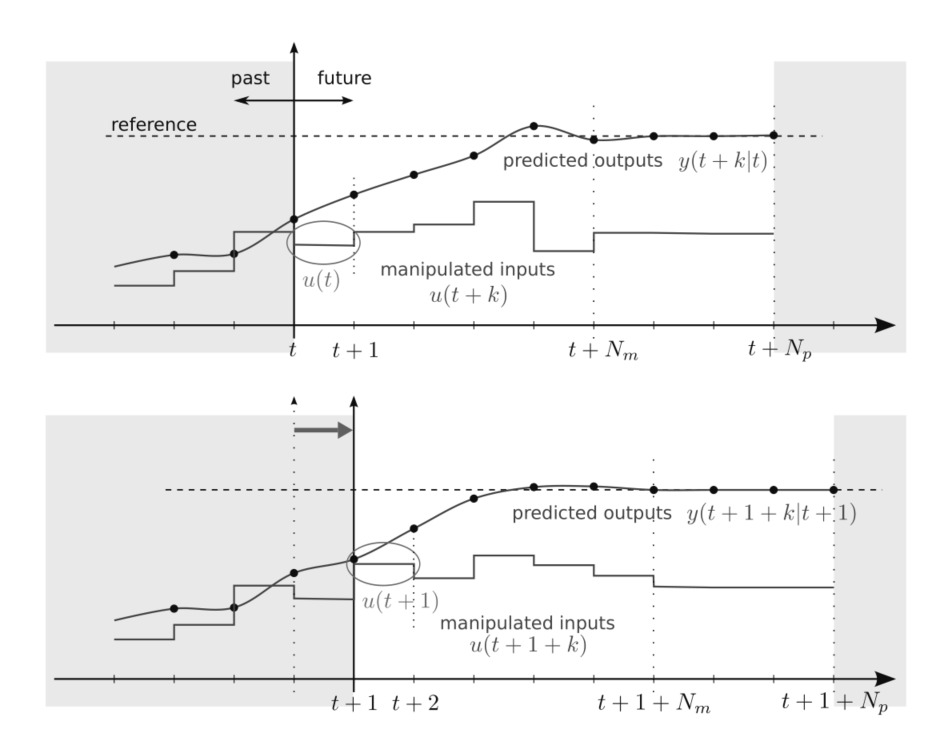
\includegraphics[width=.9\textwidth]{EMPC_PNG_Pics/RHC_gray.jpg}
        \caption{Graphycal display of receiding horison control (RHC) idea \cite{borrelli2017predictive}.}
        \label{BASICCSR:fig:RHC}
    \end{figure}

The Formulation of the optimal control problem with moving horizon \cite{goodwin2006constrained} in the system \ref{BASICMPC:equ:basic_LTI} with input and output constraints as mentioned in \ref{BASICMPC:equ:basic_LTI_constrained} with the cost function to minimize:
		
		\begin{equation}
        \begin{array}{rcl}
				J(\textbf{U},\textbf{x}(q))&=&\min_{\textbf{U}_{q\rightarrow q+N|q}}J_q(\textbf{x}(q),\textbf{U}_{q\rightarrow q+N|q})\\
                &=&\textbf{x}'_{q+N_y|q}\textbf{P}\textbf{x}_{q+N_y|q}+\sum^{N_y-1}_{k=0}\textbf{x}'_{q+k|q}\textbf{Q}\textbf{x}_{q+k|q}+\textbf{u}'_{q+k}\textbf{R}\textbf{u}_{q+k},\\
				&\textnormal{subj. to}&\textbf{x}_N\in\mathcal{X}_f,\textbf{x}_k\in\mathcal{X}^x,\textbf{u}_k\in\mathcal{U}^u\\
				&&\textbf{x}_{q|q}=\textbf{x}(q),\\
				&&\textbf{x}_{q+k+1|q}=\textbf{A}\textbf{x}_{q+k|q}+\textbf{B}\textbf{u}_{q+k},\\
				%&&\textbf{y}_{q+k|q}=\textbf{C}\textbf{x}_{q+k|q}, k\geq0,\\
				&&\textbf{u}_{q+k}=-K\textbf{x}_{q+k|q}, N_u\leq k\leq N_y,\\
        \end{array}
        \label{BASICMPC:equ:receiding_horison_problem}
    \end{equation}
		
		where $\textbf{Q}=\textbf{Q}'\geq0$, $\textbf{R}=\textbf{R}'\geq0$, $\textbf{P}\geq0$, $(\textbf{C},\textbf{A})$ is observable, and $N_u\leq N_y$, $N_c\leq N_y-1$. One trivial possibility to choose $K=0$ and $\textbf{P}$ to satisfy the Lyapunov equation:
		
		\begin{equation}
        \begin{array}{rcl}
				\textbf{P}&=&\textbf{A}'\textbf{PA}+\textbf{Q}\\
        \end{array}
        \label{BASICMPC:equ:receiding_horison_Lyapunov}
    \end{equation}
		
		This means that after $N_u$ samples the control stops and the system is evolving to an open loop form. It is obvious that the choice only makes sense if the open loop system is stable. The second option would as described with the method \ref{BASICMPC:equ:cost_function_Euclidian_recursive_twoP}, but this involves to use an unconstrained control for $N_u$ LQR samples. As a result, the MPC law calculates the optimal command sequence:
		
		\begin{equation}
        \begin{array}{rcl}
				\textbf{U}^*(q)&=&\left\{\textbf{u}^*_q,\dots,\textbf{u}^*_{q+N_u-1}\right\},\\
        \end{array}
        \label{BASICMPC:equ:receiding_optimal_sequence}
    \end{equation}
		
		and only the first control input is applied:
		
		\begin{equation}
        \begin{array}{rcl}
				\textbf{u}(q)=\textbf{u}^*_q.\\
        \end{array}
        \label{BASICMPC:equ:receiding_optimal_first}
    \end{equation}
		
		The optimal control inputs estimated for future samples are not taken into account and the algorithm is
repeated on the basis of new measurements or a new estimation of the states.	

    \subsubsection{Stability of MPC}\label{BASICCSR:sec:MPCStability}

    	The problem of closed system stability with the predictive control has been extensively studied e.g. in \cite{mayne2000constrained}, \cite{grieder2005stabilizing}. In the first generation of model based controllers, stability was achieved more experimentally by choosing parameters based on previous studies and experiences. In 1988 the Lyapunov stability method for discrete systems were introduced \cite{keerthi1988optimal}, and in 1990 for continuous systems \cite{mayne1990receding} also for continuous systems. \\
    While asymptotic convergence $\lim_{k\rightarrow\infty}\textbf{x}_k=0$ is a desirable property, it is generally not sufficient in practice. We would also like a system to stay in a small neighborhood of the origin when it is disturbed by a little. Formally this is expressed as Lyapunov stability.\\
    For the autonomous system:

    \begin{equation}
    \begin{array}{rcl}
            \textbf{x}_{k+1}&=&g(\textbf{x}_k)\\
            %&\textnormal{subj. to}&g(0)=0,
        \end{array}
        \label{BASICMPC:equ:autonom_system}
    \end{equation}

    where $g(0)=0$. The definition of Lyapunov stability is for the equilibrium point $\textbf{x}=0$ of system \ref{BASICMPC:equ:autonom_system} is:
    \begin{itemize}
    \item stable if, for each $\epsilon>0$, there is a $\varphi>0$ such that:
        \begin{equation}
        \begin{array}{c}
                \norm{\textbf{x}_0}<\varphi\textnormal{ s.t.: }\norm{\textbf{x}_k}<\epsilon,\textnormal{ }\forall k\geq0.
            \end{array}
            \label{BASICMPC:equ:lyapunov_1}
        \end{equation}

    \item unstable if not stable

    \item asymptotically stable if in the set $\boldsymbol{\Omega}\subseteq\mathbb{R}^n$ if its stable and:
       \begin{equation}
        \begin{array}{c}
                \lim_{k\rightarrow\infty}\textbf{x}_k=0,\textnormal{ }\forall\textbf{x}_0\in\boldsymbol{\Omega}.
            \end{array}
            \label{BASICMPC:equ:lyapunov_2}
        \end{equation}

    \item globally asymptotically stable if it is asymptotically stable and $\boldsymbol{\Omega}=\mathbb{R}^n$

    \item exponentially stable if it is stable and there exist constants $\chi>0$ and $\psi\in(0,1)$ such that:
    \begin{equation}
        \begin{array}{c}
                \norm{\textbf{x}_0}<\varphi\textnormal{ s.t.: }\norm{\textbf{x}_k}\leq\chi\norm{\textbf{x}_0}\psi^k,\textnormal{ }\forall k\geq0.
            \end{array}
            \label{BASICMPC:equ:lyapunov_3}
        \end{equation}


    \end{itemize}

    Usually to show Lyapunov stability of the origin for a particular system one constructs a so called Lyapunov function, i.e., a function satisfying the conditions of the following theorem:\\
    Consider the equilibrium point $\textbf{x}=0$ of system \ref{BASICMPC:equ:autonom_system}. Let $\boldsymbol{\Omega}\subset\mathbb{R}^n$ be a closed and bounded set containing the origin. Assume there exists a function $V:\mathbb{R}^n\rightarrow\mathbb{R}$ continuous at the origin, finite for every $\textbf{x}\in\boldsymbol{\Omega}$ and such that:

    \begin{subequations}
    \label{BASICMPC:equ:lyapunov_4_1}
        \begin{align}
                V(0)=0 \label{BASICMPC:equ:lyapunov_4_1_a}\\
                V(\textbf{x})>0,\textnormal{ }\forall\textbf{x}\in\boldsymbol{\Omega}\textbackslash\{0\} \label{BASICMPC:equ:lyapunov_4_1_b}\\
                V(\textbf{x}_{k+1})-V(\textbf{x}_{k})\leq-\chi(\textbf{x}_k),\textnormal{ }\forall\textbf{x}\in\boldsymbol{\Omega}\textbackslash\{0\}, \label{BASICMPC:equ:lyapunov_4_1_c}
        \end{align}
    \end{subequations}

     where $\chi:\mathbb{R}^n\rightarrow\mathbb{R}$ is a continuous positive definite function, then $\textbf{x}=0$ is asymptotically stable. As such a function satisfying \ref{BASICMPC:equ:lyapunov_4_1} is called a Lyapunov function.\\
     A similar theorem can be derived for global asymptotic stability i.e.: $\boldsymbol{\Omega}=\mathbb{R}^n$:
     Consider the equilibrium point $\textbf{x}=0$ of system \ref{BASICMPC:equ:autonom_system}. Let $\boldsymbol{\Omega}\subset\mathbb{R}^n$ be a closed and bounded set containing the origin. Assume there exists a function $V:\mathbb{R}^n\rightarrow\mathbb{R}$ continuous at the origin, finite for every $\textbf{x}\in\boldsymbol{\Omega}$ and such that:

     \begin{subequations}
    \label{BASICMPC:equ:lyapunov_4_2}
        \begin{align}
                \norm{\textbf{x}}\rightarrow\infty,\textnormal{ s.t.: }V(\textbf{x})\rightarrow\infty \label{BASICMPC:equ:lyapunov_4_2_a}\\
                V(0)=0 \label{BASICMPC:equ:lyapunov_4_2_b}\\
                V(\textbf{x})>0,\textnormal{ }\forall\textbf{x}\neq0 \label{BASICMPC:equ:lyapunov_4_2_c}\\
                V(\textbf{x}_{k+1})-V(\textbf{x}_{k})\leq-\chi(\textbf{x}_k),\textnormal{ }\forall\textbf{x}\neq0, \label{BASICMPC:equ:lyapunov_4_2_d}
            \end{align}
            \end{subequations}
     where $\chi:\mathbb{R}^n\rightarrow\mathbb{R}$ is a continuous positive definite function, then $\textbf{x}=0$ is globally asymptotically stable.\\
     For linear systems a simple and effective Lyapunov function can be:

     \begin{equation}
        \begin{array}{rcl}
                V(\textbf{x})&=&\textbf{x}'\textbf{P}\textbf{x},\textbf{P}\succ 0,\\
            \end{array}
            \label{BASICMPC:equ:lyapunov_5}
        \end{equation}

    In order to test the satisfaction of the last point of \ref{BASICMPC:equ:lyapunov_4_2}, we compute:

    \begin{equation}
        \begin{array}{rcl}
                V(\textbf{x}_{k+1})-V(\textbf{x}_{k})&=&\textbf{x}'_{k+1}\textbf{P}\textbf{x}_{k+1}-\textbf{x}'_{k}\textbf{P}\textbf{x}_{k}\\
                &=&\textbf{x}'_{k}(\textbf{A}'\textbf{P}\textbf{A})\textbf{x}_{k}-\textbf{x}'_{k}\textbf{P}\textbf{x}_{k}\\
                &=&\textbf{x}'_{k}(\textbf{A}'\textbf{P}\textbf{A}-\textbf{P})\textbf{x}_{k},
            \end{array}
            \label{BASICMPC:equ:lyapunov_6}
        \end{equation}

    therefore, if \ref{BASICMPC:equ:lyapunov_5} holds true then:

    \begin{equation}
        \begin{array}{rcl}
                 \textbf{A}'\textbf{P}\textbf{A}-\textbf{P}&=&-\textbf{Q},\textbf{Q}\succ 0,\\
            \end{array}
            \label{BASICMPC:equ:lyapunov_7}
        \end{equation}

which is referred as discrete time Lyapunov equation.
\section[Predictive control of a CSR]{Constrained, explicit predictive control for current source buck-type rectifiers}\label{EMPC:sec:main}

As mentioned in section \oldref{BASICCSR:sec:CSR_Literature} current source rectifiers (CSR) play a major role in industrial instrumentation. They are invaluable, in the fields of direct power control, torque control, or power injection is required.\\
 \hlc[PT]{In the third thesis, I propose an explicit model based predictive control scheme realised on a classic CSR (or buck-type rectifier) control structure. The device as the name suggests utilizes three phase alternating current waveform, obtained from domestic three phase source, to create a steady direct current on the output poles. This structure was described in section} \oldref{BASICCSR:sec:CSR}\hlc[PT]{, where the topology and waveform formulation is written in detail. Also worth mention that the modelled devices's equations (described in section} \oldref{EMPC:sec:ModelofCSR})\hlc[PT]{ are not entirely in the linear domain.}\\
  \hlc[PT]{The employed control structure (section }\oldref{EMPC:sec:DCside})\hlc[PT]{ is unique in a sense, since classic model based predictive control was not part of the power electronic domain recently. The high frequency switching periods and dynamical demand renders classic MPCs ineffective due to they massive calculation demand. However, if the control space is mapped and an effective search pattern is utilized, the feasibility could be guarantied. Also since the control structure relies on physical parameters the structure of choice supports embedded constraint handling(described in section} \oldref{BASICCSR:sec:OptimalControl}) \hlc[PT]{which is essential in electric power conversion realisations.}\\
  \hlc[PT]{The goal of the control is two fold. On one hand the goal is to reach the steady state current reference, with minimal overshoot, at the output poles as fast as possible with a resistive load assumed. On the other, the reactive power and process noise on the network's side shall be also minimized.}\\
		
\subsection{Modeling}\label{EMPC:sec:Modeling}

Understandably, model based controllers require the system's model the ought to control, or supervise. In this case the most common structure of a CSR is chosen, with inductive and capacitive filtering on both ends. The differential equations are constructed based on Kirchoff's law and then presented as a state space model for further examination.

\subsubsection{Mathematical modeling of the CSR}\label{EMPC:sec:ModelofCSR}

    The structure of the classical three phase buck-type current source rectifier (CSR) is presented in \ref{EMPC:fig:network}. \hlc[PT]{The purpose of such a device is provide a continuous direct current at the output ($i_{dc}$) but instead of the widely used boost type counterparts, the voltage can be consideraby lower, making ideal for high current operations like induction heating. The device's detailed contexture can be observed in section} \oldref{BASICCSR:sec:CSR}. \hlc[PT]{Basically, a finite configuration of switching states with high enough frequency consists a continuous current flow of direct- at the output poles and alternating current at the input poles. This is reached via filtering the high dynamic ripples with low pass filtering realised with LC components.} In continuous current mode, the differential equations corresponding to the CRS’s inductor currents and capacitor voltages (\hlc[PT]{obtained straightforwardly via Kirchoff's law.}) are the following:

    \begin{figure}[!ht]
        \centering
        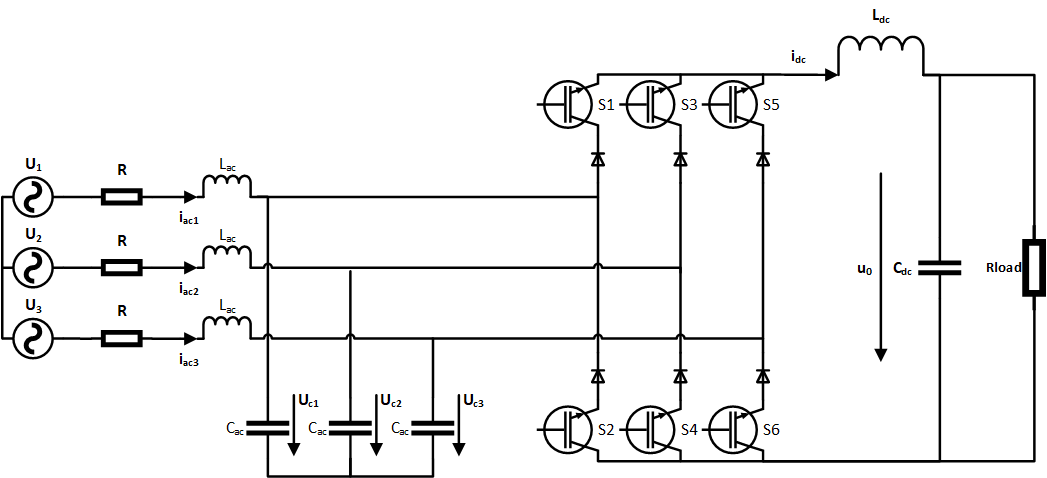
\includegraphics[width=\textwidth]{EMPC_PNG_Pics/circuit.png}
        \caption{Circuit diagram of the three-phase buck-type rectifier with insulated gate bipolar transistors (IGBTs).}
        \label{EMPC:fig:network}
    \end{figure}
		
        \begin{equation}
        \begin{array}{rcl}
            L_{ac}\dot{i_{ac_p}}&=&u_p-u_{c_p}-Ri_{ac_p}\\
            C_{ac}\dot{u_{c_p}}&=&i_{ac_p}-\delta_pi_{dc}\\
            L_{dc}\dot{i_{dc}}&=&(\sum_{p=1}^{3}\delta_pu_{c_p})-u_0\\
            C_{dc}\dot{u_0}&=&i_{dc}-\frac{u_0}{R_{load}}\\
        \end{array}
        \label{EMPC:equ:abc_eqn}
    \end{equation}

    where $p\in\{1,2,3\}$ is the index of three phases and $\delta_p$ describes the conduction state of the rectifier leg p \ref{EMPC:equ:delta_set}.

    \begin{equation}
        \begin{array}{rcl}
            \delta_p&=&\begin{Bmatrix}
                \textrm{1 if the upper transitor is ON}\\
                \textrm{-1 if the lower transistor is ON}\\
                \textrm{0 if both are ON or OFF}
            \end{Bmatrix}
        \end{array}
        \label{EMPC:equ:delta_set}
    \end{equation}

    Converting the components in the stationary (Clarke) frame (displayed in section \oldref{BASICCSR:sec:Clarke}) of the space phasors of the three-phase quantities, from \ref{EMPC:equ:abc_eqn} it results:

    \begin{equation}
        \begin{array}{rcl}
            L_{ac}\dot{i_{ac_\alpha}}&=&u_\alpha-u_{c_\alpha}-Ri_{ac_\alpha}\\
            L_{ac}\dot{i_{ac_\beta}}&=&u_\beta-u_{c_\beta}-Ri_{ac_\beta}\\
            C_{ac}\dot{u_{c_\alpha}}&=&i_{ac_\alpha}-\delta_\alpha i_{dc}\\
            C_{ac}\dot{u_{c_\beta}}&=&i_{ac_\beta}-\delta_\beta i_{dc}\\
            L_{dc}\dot{i_{dc}}&=&1.5(\delta_\alpha u_{c_\alpha}+\delta_\beta u_{c_\beta})-u_0\\
            C_{dc}\dot{u_0}&=&i_{dc}-\frac{u_0}{R_{load}}\\
        \end{array}
        \label{EMPC:equ:abc_alfabeta}
    \end{equation}

    Equation \ref{EMPC:equ:abc_alfabeta} is transformed to the synchronous reference (Park) frame (displayed in section \oldref{BASICCSR:sec:Park}) rotating with the $u_{c_d}$ capacitor voltage space vector. The resulting mathematical model is thus:

    \begin{equation}
        \begin{array}{rcl}
            L_{ac}\dot{i_{ac_d}}&=&u_d-u_{c_d}-Ri_{ac_d}+\omega_s L_{ac}i_{ac_q}\\
            L_{ac}\dot{i_{ac_q}}&=&u_d-u_{c_q}-Ri_{ac_q}-\omega_s L_{ac}i_{ac_d}\\
            C_{ac}\dot{u_{c_d}}&=&i_{ac_d}-\delta_di_{dc}+\omega_s C_{ac}u_{c_q}\\
            C_{ac}\dot{u_{c_q}}&=&i_{ac_q}-\delta_qi_{dc}-\omega_s C_{ac}u_{c_d}\\
            L_{dc}\dot{i_{dc}}&=&1.5(\delta_d u_{c_d}+\delta_q u_{c_q})-u_0\\
            C_{dc}\dot{u_0}&=&i_{dc}-\frac{u_0}{R_{load}}\\
        \end{array}
        \label{EMPC:equ:abc_dq}
    \end{equation}

    where $\omega_s$ represents the network voltage vector’s angular velocity.

    \subsubsection{Model simplification}\label{EMPC:sec:Simplification}

    Notice, that the sixth-order ODE model \ref{EMPC:equ:abc_dq} is bilinear in its states and inputs because of the product terms (e.g.: $\delta_di_{dc}$). As such, using design methods for linear systems is not straightforward. The high complexity given by the system’s order is another problem to tackle. For designing classic MPC, linear, low-order equation systems are favorable. Hence simplification of the model would bring noteworthy benefits, making the MPC design more straightforward, when a linear system resulted.
    Since the three phase alternating current (AC) and the direct current (DC) side’s time constants differ significantly (as in the AC: $\omega_{ac}=\frac{1}{\sqrt{L_{ac} C_{ac}}}\cong5.7\cdot10^3$ rad/s, and on the DC: $\omega_{dc}=\frac{1}{\sqrt{L_dc C_dc}}\cong2.8\cdot10^2$ rad/s, see Table \ref{EMPC:tbl:params}. for reference). Thus, the differential equations can be separated into two sets, and the control of the AC and DC sides can be decoupled as described in \cite{ahmed2014model}. The AC side model results as follows:


    \begin{equation}
        \begin{array}{rcl}
            \begin{bmatrix}
                \dot{i_{ac_d}}\\
                \dot{i_{ac_q}}\\
                \dot{u_{c_d}}\\
                \dot{u_{c_q}}
            \end{bmatrix}&=&
            \begin{bmatrix}
                -\frac{R}{L_{ac}}   &\omega &-\frac{1}{L_{ac}}  &0\\
                -\omega   &-\frac{R}{L_{ac}} &0  &-\frac{1}{L_{ac}}\\
                \frac{1}{C_{ac}}   &0 &0  &\omega\\
                0   &\frac{1}{C_{ac}} &-\omega  &0
            \end{bmatrix}
            \begin{bmatrix}
                i_{ac_d}\\
                i_{ac_q}\\
                u_{c_d}\\
                u_{c_q}
            \end{bmatrix}+
            \begin{bmatrix}
                \frac{u_d}{L_{ac}}\\
                \frac{u_q}{L_{ac}}\\
                -\frac{\delta_di_{dc}}{C_{ac}}\\
                -\frac{\delta_qi_{dc}}{C_{ac}}
            \end{bmatrix}
        \end{array}
        \label{EMPC:equ:mtx_AC}
    \end{equation}

    Looking at the state matrix it can be further stated that there are only weak couplings between the $d$ and $q$ synchronous reference frame components. This allows to handle them separately, and later to design separate control for each.
    The equation system describing the DC side dynamics is the following:

    \begin{equation}
        \begin{array}{rcl}
            \begin{bmatrix}
                \dot{i_{dc}}\\
                \dot{u_{0}}
            \end{bmatrix}&=&
            \begin{bmatrix}
                0&  -\frac{1}{L_{dc}}\\
                \frac{1}{C_{dc}}&   -\frac{1}{R_{load}C_{dc}}
            \end{bmatrix}
            \begin{bmatrix}
                i_{dc}\\
                u_0
            \end{bmatrix}+
            \begin{bmatrix}
                \frac{1.5}{L_{dc}}(\delta_du_{c_d}+\delta_qu_{c_q})\\
                0
            \end{bmatrix}
        \end{array}
        \label{EMPC:equ:mtx_DC}
    \end{equation}

    It can be noticed that, with the AC and DC model separation, bilinearity disappears, since the binding coefficients are present only in the input $(\textbf{u})$ of the DC state space model \ref{EMPC:equ:mtx_DC}. Consequently, all equations are linear and with a considerably lower order, making control design much easier and allowing for the application of linear design methods. For the DC side dynamics, the linear time invariant differential equation system’s matrices can be identified for predictive control design purposes:

    \begin{equation}
        \begin{array}{rcl}
            \textbf{x}&=&\begin{bmatrix}
                i_{dc}\\
                u_0
            \end{bmatrix},\\
            \textbf{u}&=&(\delta_d u_{c_d}+\delta_q u_{c_d}),\\
            \textbf{y}&=&u_0,\\
            \textbf{A}&=&\begin{bmatrix}
                0&  -\frac{1}{L_{dc}}\\
                \frac{1}{C_{dc}}&   -\frac{1}{R_{load}C_{dc}}
            \end{bmatrix},\\
            \textbf{B}&=&\begin{bmatrix}
                i_{dc}\\
                u_0
            \end{bmatrix},\\
            \textbf{C}&=&\begin{bmatrix}0 &1\end{bmatrix}.
        \end{array}
        \label{EMPC:equ:mtx_ctrl}
    \end{equation}

    where \textbf{x}, \textbf{u} and \textbf{y} are the state, input and output vectors of the DC-side system, and \textbf{A}, \textbf{B} and \textbf{C} are the state, input and output matrices.
    The circuit parameters used for the implementation of the control structure based on this model are presented in Table \ref{EMPC:tbl:params}.

    \begin{table}[]
    \center
		\caption{The applied parameters in model and controller design}
        \begin{tabular}{|l|l|}
        \hline
        Parameter      & Value  \\ \hline
        \textbf{R}     & 0.3 $\Omega$ \\ \hline
        \textbf{Rload} & 10 $\Omega$  \\ \hline
        \textbf{Lac}   & 1 mH    \\ \hline
        \textbf{Ldc}   & 30 mH   \\ \hline
        \textbf{Cac}   & 30 $\mu$F   \\ \hline
        \textbf{Cdc}   & 400 $\mu$F  \\ \hline
        \textbf{f}     & 50 Hz   \\ \hline
        \textbf{fpwm}  & 20 kHz  \\ \hline
        \textbf{Un}    & 400 V   \\ \hline
        \end{tabular}
        \label{EMPC:tbl:params}
    \end{table}

\subsubsection{Control structure}\label{EMPC:sec:ControlStruct}

    \hlc[PT]{The described structure of the CSR naturally can only be interpreted in a power electric context. As such the control requirements of the system is shifted respectfully in such a direction that those requirements are met within physical constrains also, within the dissertation's scope. As mentioned in the previous chapter, the modeling of the CSR enables to handle the control goal from two somewhat disjunct perspective. With this in mind, the control requirements can be placed on three categories. }\hlc[PT]{With }\ref{EMPC:equ:mtx_ctrl} \hlc[PT]{in mind these are the following:}

    \begin{itemize}
    \item \hlc[PT]{\textbf{AC side:} Minimize current ripple and reactive power from the network's measurement point (at the voltage sources on the topology). In this scenario the domestic network is assumed ideal, aka. the voltage source is an ideal three phase sinusoidal waveform with $50Hz$ network frequency. The disturbance is coming exclusively form the LC filter's oscillation, and from the PWM switching behaviour.}
    \item \hlc[PT]{\textbf{DC side:} Reach the reference of $u_0^*$ the fastest possible with minimal overshoot, and steady state error on the resistive load's poles. The fewer number of critical regions, and less horizon length of the EMPC shall be chosen, since these are correlating between the calculation requirements of possible experimental setup.}
    \item \hlc[PT]{\textbf{Modulation:} The modulation shall transform the reference current into the optimal switching state, which was permitted by the modulation table. Also, the desired switching sequence shall be conducted with minimum amount of switching used.}
    \end{itemize}
    Using the separation of the AC side and DC side controllers, the control structure depicted in Fig. \ref{EMPC:fig:ControlStruct}. is proposed.

    \begin{figure}[!ht]
        \centering
        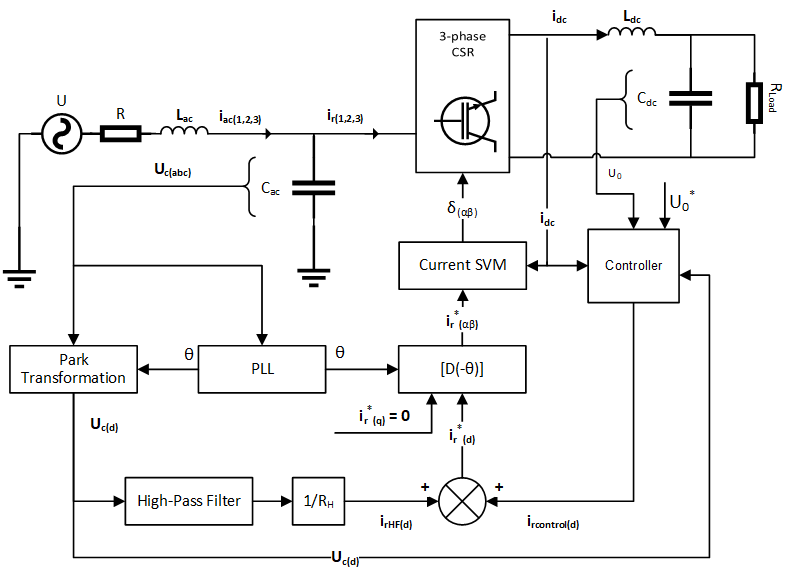
\includegraphics[width=\textwidth]{EMPC_PNG_Pics/ControlStructure.png}
        \caption{Block diagram of the control structure.}
        \label{EMPC:fig:ControlStruct}
    \end{figure}

    The controllers operate in the synchronous frame of the AC filter capacitor voltages $u_{c_{(1,2,3)}}$, and the rectifier input currents $i_{r_{(1,2,3)}}$ are in phase with the capacitor voltages.
    The current reference $i^*_{\alpha\beta}$ supplied to the space vector modulation unit in the stationary frame, is obtained by coordinate transformation $[D(-\Theta)]$ (or Park to Clarke transformation) of the current reference \ref{EMPC:equ:sync_ctrl} delivered by the current controllers in the synchronous frame.

    \begin{equation}
        \begin{array}{rcl}
            \begin{Bmatrix}
                i^*_{r_d}=i_{rcontrol_d}+i_{rHF_d}\\
                i^*_{r_q}=0
            \end{Bmatrix}
        \end{array}
        \label{EMPC:equ:sync_ctrl}
    \end{equation}

    In \ref{EMPC:equ:sync_ctrl}, $i_{rcontrol_d}$ represents the output of the DC voltage controller, while $i_{rHF_d}$ represents the damping current, proportional with the high frequency component of the filter capacitor voltage (the fundamental component of the capacitor voltage in the stationary frame becomes a DC component in the synchronous frame). The DC and AC side control units are explained in more detail in the following sections, and the performance of the control structure is evaluated.
		
\subsection{Control}\label{EMPC:sec:Control}

    In this section the model based control algorithm is explained, used on the DC side, followed by a simpler AC side active damping.

\subsubsection{DC-side explicit model predictive control} \label{EMPC:sec:DCside}

    Model predictive control (MPC) is an efficient and systematic method for solving complex multi-variable constrained optimal control problems \cite{vajda2017limiting}. The basic notions of MPC is explained in section \oldref{BASICCSR:sec:MPC}, where the MPC control law is explained, namely, is based on the “receding horizon formulation”, where the model’s assumed behavior is calculated for a number of $N$ steps, where $N$ stands for the horizon’s length. Only the first step of the computed optimal input is applied in each iteration. The remaining steps of the optimal control input are discarded and a new optimal control problem (explained in section \oldref{BASICCSR:sec:LQR}) is solved at the next sample time. Using this approach, the receding horizon policy provides the controller with the desired feedback characteristics, although with high order systems the computational effort is considerably demanding since all the steps should be taken in to account on the specified horizon in every iteration.\\
		With Explicit MPC (EMPC), the discrete time constrained optimal control problem is reformulated as multi-parametric linear or quadratic programming. As explained in section \oldref{BASICCSR:sec:OptimalControl}, the optimization problem can be solved off-line, making it much more feasible from the perspective of the optimal control task. The optimal control law is a piecewise affine function of the states, and the resulting solution is stored in a pre-calculated lookup table. The parameter space, or the state-space is partitioned into critical regions. The real-time implementation consists in searching for the active critical region, where the measured state variables lie, and in applying the corresponding piecewise affine control law to achieve the desired dynamics.
    In order to introduce the MPC implementation, let us consider a linear discrete time system \ref{EMPC:equ:DiscreteStateSpace} derived with the discretisation of system \ref{EMPC:equ:mtx_DC} with zero-order hold method, where control inputs are assumed piecewise constant over the simulation sample time $T_s=\frac{1}{f_s}$ :

    \begin{equation}
        \begin{array}{rcl}
            \textbf{x}(t+1)&=&\textbf{A}_d\textbf{x}(t)+\textbf{B}_d\textbf{u}(t)\\
            \textbf{y}(t)&=&\textbf{C}_d\textbf{x}(t)
        \end{array}
        \label{EMPC:equ:DiscreteStateSpace}
    \end{equation}

    where $\textbf{A}_d$, $\textbf{B}_d$, $\textbf{C}_d$ are the matrices of the discretised system derived from \ref{EMPC:equ:mtx_ctrl}. With system \ref{EMPC:equ:DiscreteStateSpace} is linear and time invariant, MPC design can be followed. The following constraints have to be satisfied:

    \begin{equation}
        \begin{array}{r}
            \textbf{y}_{min}\leq\textbf{y}(t)\leq\textbf{y}_{max},\\
            \textbf{u}_{min}\leq\textbf{u}(t)\leq\textbf{u}_{max}
        \end{array}
        \label{EMPC:equ:contraint_desc}
    \end{equation}

    where $t>0$, $\textbf{x}\in \mathbb{R}^n$, $\textbf{u}\in \mathbb{R}^m$, $\textbf{y}\in \mathbb{R}^p$. The MPC solves the following constrained optimization problem \cite{rivera2013predictive}:

    \begin{equation}
        \begin{array}{rcl}
           \displaystyle \min_{U=\{u_t\dots u_t+N_u-1\}}J(\textbf{u},\textbf{x}(t))&=&\sum^{N_y-1}_{k=0}(\textbf{x}^T_{t+N_y|t}\textbf{Q}\textbf{x}_{t+N_y|t}+
           \textbf{u}^T_{t+k}\textbf{R}\textbf{u}_{t+k})\\
        \end{array}
        \label{EMPC:equ:optim_problem}
    \end{equation}

    subject to:

    \begin{equation}
        \begin{array}{l}
            \textbf{x}_{min}\leq\textbf{x}_{t+k|t}\leq\textbf{x}_{max},\,k=1,\dots,N_c-1\\
            \textbf{u}_{min}\leq\textbf{u}_{t+k|t}\leq\textbf{u}_{max},\,k=1,\dots,N_c-1\\
            \textbf{x}_{t|t}=\textbf{x}(t),\,\textbf{u}_{t|t}=\textbf{u}(t)\\
            \textbf{x}_{t+k+1|t}=\textbf{A}_d\textbf{x}_{t+k|t}+\textbf{B}_d\textbf{u}_{t+k|t}\\
            \textbf{y}_{t+k|t}=\textbf{C}_d\textbf{x}_{t+k|t}\\
            \textbf{u}_{t+k|t}=-K\textbf{x}_{t+k|t},\,k\geq0\\
        \end{array}
        \label{EMPC:equ:optim_problem_constr}
    \end{equation}
There the formulation of such problem is described in detail in chapter \ref{BASICCSR:sec:OptimalControl}.\\
    This problem is solved at each time instant $t$, where $\textbf{x}_{t+k\vert t}$ denotes the state vector predicted at time $t+k$, obtained by applying the input sequence $\textbf{u}_{t|t}...\textbf{u}_{t|t+1}$ to model \ref{EMPC:equ:quadratic_regions}, starting from the state $\textbf{x}_{t|t}$. Further, it is assumed that $Q$ and $R$, are symmetric positive semidefinite $(\textbf{Q}_w=\textbf{Q}_w^T\geq0$, $\textbf{R}_w=\textbf{R}_w^T>0)$ and $K$ is a feedback gain. Further, $N_y,N_u,N_c$ are the output, input and constraint horizons, respectively.
    Using the model for predicting the future behavior of the system and with some appropriate substitution and variable manipulation which basic notions showed in section \oldref{BASICCSR:sec:MPC}, the problem \ref{EMPC:equ:optim_problem},\ref{EMPC:equ:optim_problem_constr} can be transformed to the standard multi parametric quadratic programming form, as described in \cite{rivera2013predictive}:

    \begin{equation}
        \begin{array}{rcl}
            J^*(\textbf{x}(t))&=&\min_{\textbf{z}}J(\textbf{x},\textbf{z})=\frac{1}{2}\textbf{z}'\textbf{H}\textbf{z}
        \end{array}
        \label{EMPC:equ:quadratic_program}
    \end{equation}

    where subject to:

    \begin{equation}
        \begin{array}{rcl}
            \textbf{Gz}&\leq&\textbf{w}+\textbf{S}\textbf{x}(t)
        \end{array}
        \label{EMPC:equ:quadratic_inequality}
    \end{equation}

    where the matrices $\textbf{H}$, $\textbf{G}$, $\textbf{w}$, $\textbf{S}$ result directly from the coordinate transformations described in \ref{BASICCSR:sec:OptimalControl}. The solution of the quadratic optimization problem for each critical region has the form:

    \begin{equation}
        \begin{array}{rcl}
            \textbf{u}^*&=&\textbf{F}_i\textbf{x}+\textbf{g}_i
        \end{array}
        \label{EMPC:equ:quadratic_regions}
    \end{equation}

    and the critical region is described by:

    \begin{equation}
        \begin{array}{rcl}
            \mathcal{C}_{reg_i}&=&\{\textbf{x}\in \mathbb{R}^n|\textbf{H}_i\textbf{x}\leq \textbf{K}_i\}
        \end{array}
        \label{EMPC:equ:quadratic_critical}
    \end{equation}

    Thus, the explicit MPC controller is completely characterized by the set of parameters:

    \begin{equation}
        \begin{array}{l}
            \{\textbf{F}_i,\textbf{g}_i,\textbf{H}_i,\textbf{K}_i|i=1\dots N\}
        \end{array}
        \label{EMPC:equ:quadratic_set}
    \end{equation}

    In case of the discrete time system resulting from \ref{EMPC:equ:mtx_ctrl}, for sampling time equal with the switching period $T_s=5\cdot10^{-5}$  s, the problem defined to be solved by MPC is the minimization of the quadratic cost function \ref{EMPC:equ:DiscreteStateSpace} for:

    \begin{equation}
    \hlcmath{PT}{
        \begin{array}{l}
            \textbf{R}_w=\begin{bmatrix}
                1\\
            \end{bmatrix},
            \textbf{Q}_w=\begin{bmatrix}
                5\cdot10^{-5}& 0\\
                0& 5\cdot10^{-5}\\
            \end{bmatrix},
            N_y=N_u=N_c=4.
        \end{array}}
        \label{EMPC:equ:quadratic_mtx_set}
    \end{equation}

    Since $N_y,N_u,N_c$ take the same value, they will be substituted by $N$.
    The constraints defined based on the rated power of the CSR $P_n=2500$ W, are:

    \begin{equation}
        \begin{array}{rcl}
            0\leq&i_{dc}&\leq 50A\\
            0\leq&u_{0}&\leq 500V.
        \end{array}
        \label{EMPC:equ:numeric_constraints}
    \end{equation}

    The state space partition resulting from this problem has \hlcmath{PT}{10} critical regions, which can be observed in Fig. \ref{EMPC:fig:regions}.

    \begin{figure}[!ht]
        \centering
        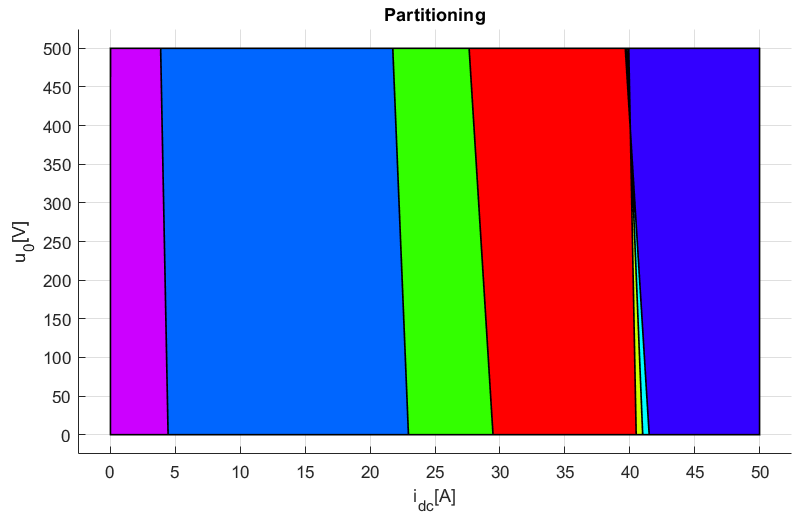
\includegraphics[width=\textwidth]{EMPC_PNG_Pics/Regions2_trans.png}
        \caption{\hlcmath{PT}{\textnormal{State space partitioning over the determined constraints.}}}
        \label{EMPC:fig:regions}
    \end{figure}

    From the basis of the discretised model \ref{EMPC:equ:DiscreteStateSpace}, the given constraints \ref{EMPC:equ:numeric_constraints}, and horizon \ref{EMPC:equ:numeric_constraints} the cost function \ref{EMPC:equ:optim_problem} is established via the MPT toolbox \cite{MPT3} and uaastrom2013computeraastrom2013computerzhang2015simplifiedsed in the generated controller for the EMPC design [29], [31]. The controller is created as a compliable S-function in the Matlab/Simulink environment and its place in the control structure can be observed in Fig. \ref{EMPC:fig:MPCStructure}. as the EMPC controller.
    The output of the MPC controller is the control variable obtained via solving \ref{EMPC:equ:optim_problem_constr} and
    $u_{MPC}=(\delta_du_{c_d}+\delta_qu_{c_q})$, from which the current reference can be calculated using \ref{EMPC:equ:numeric_constraints}. The quadrature component $u_{c_q}$ is zero in the synchronous frame of the filter capacitor voltage.


    \begin{equation}
        \begin{array}{rcl}
            i_{rMPC_{d}}&=&\frac{u_{MPC}}{u_{c_d}}\cdot i_{dc}
        \end{array}
        \label{EMPC:equ:direct_controlval}
    \end{equation}

    \begin{figure}[!ht]
        \centering
        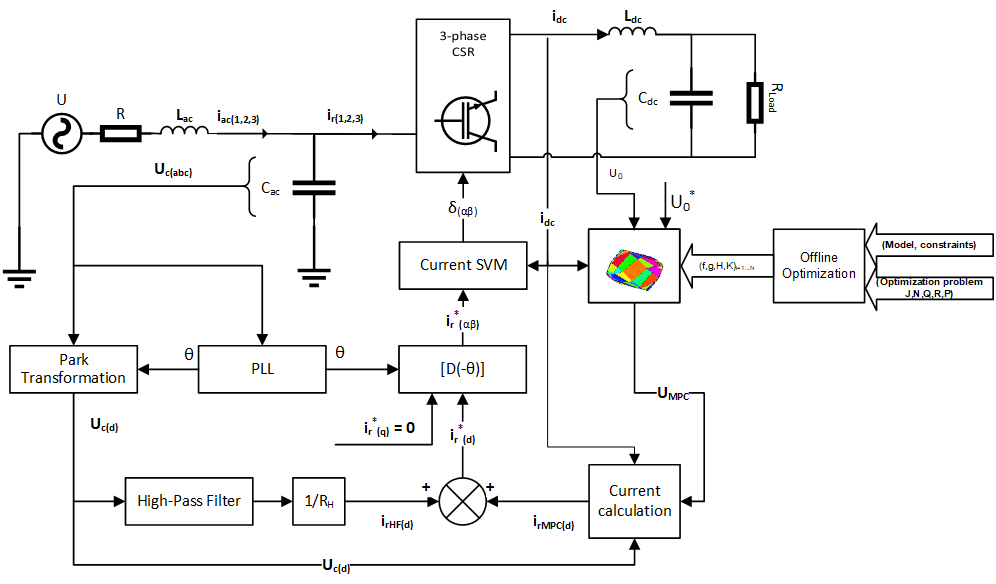
\includegraphics[width=\textwidth]{EMPC_PNG_Pics/MPCStructure.png}
        \caption{The control structure of the CSR, with MPC controller on the DC side.}
        \label{EMPC:fig:MPCStructure}
    \end{figure}

\subsubsection{Active AC-side damping}\label{EMPC:sec:ACdamping}

    The CSR requires a voltage supply on the AC side. Taking the inductive character of the mains into consideration, the presence of a three-phase capacitor bank at the input of the CSR is a must. The most convenient is to use three-phase LC filtering with inductors on the lines and star connected capacitors resembling those in Fig. \ref{EMPC:fig:network}, although the resonance phenomena between these components can still cause difficult problems.\\
    \hlc[PT]{Let us consider the AC side differential equation of the CSR from} \ref{EMPC:equ:mtx_AC}:

    \begin{equation}
    \hlcmath{PT}{
        \begin{array}{rcl}
            \begin{bmatrix}
                \dot{i_{ac_d}}\\
                \dot{i_{ac_q}}\\
                \dot{u_{c_d}}\\
                \dot{u_{c_q}}
            \end{bmatrix}&=&
            \begin{bmatrix}
                -\frac{R}{L_{ac}}   &\omega &-\frac{1}{L_{ac}}  &0\\
                -\omega   &-\frac{R}{L_{ac}} &0  &-\frac{1}{L_{ac}}\\
                \frac{1}{C_{ac}}   &0 &0  &\omega\\
                0   &\frac{1}{C_{ac}} &-\omega  &0
            \end{bmatrix}
            \begin{bmatrix}
                i_{ac_d}\\
                i_{ac_q}\\
                u_{c_d}\\
                u_{c_q}
            \end{bmatrix}+
            \begin{bmatrix}
                \frac{u_d}{L_{ac}}\\
                \frac{u_q}{L_{ac}}\\
                -\frac{\delta_di_{dc}}{C_{ac}}\\
                -\frac{\delta_qi_{dc}}{C_{ac}}
            \end{bmatrix}\nonumber.
        \end{array}}
        %\label{EMPC:equ:mtx_AC}
    \end{equation}

    \hlc[PT]{The above equation set is representing the AC dynamics well, however, since the physical system is compliant to some boundaries, further simplification can be obtained as displayed by }\cite{zhang2015simplified}\hlc[PT]{. The capacitor's voltage's d-axis can be aligned with the q-axis, as:}

    \begin{equation}
    \hlcmath{PT}{
        \begin{array}{rcl}
        u_{c_q}&=&0\\
        \end{array}}
        \label{EMPC:equ:reduced_ucq}
    \end{equation}

    \hlc[PT]{Since the time constant difference between AC and DC side, described in} \oldref{EMPC:sec:Simplification}\hlc[PT]{, and the large difference between $L_{ac}$ and $L_{dc}$, displayed in Table} \ref{EMPC:tbl:params}\hlc[PT]{. Also $i_{dc}$ can be approximated as an $I_{dc}$ constant (modulated by $\delta_d$), and neglecting small couplings such $\omega L_{ac}$, and $\omega C_{ac}$, the AC side model looks like this:}

    \begin{equation}
    \hlcmath{PT}{
        \begin{array}{rcl}
        L_{ac}\dot{i_{ac_d}}&=&u_d-u_{c_d}\\
        L_{ac}\dot{i_{ac_q}}&=&u_q\\
        C_{ac}\dot{u_{c_d}}&=&i_d-\delta_dI_{dc}\\
        0&=&i_q-\delta_qI_{dc},\\
        \end{array}}
        \label{EMPC:equ:reduced_AC}
    \end{equation}

    \hlc[PT]{Such as in} \ref{EMPC:equ:reduced_AC}\hlc[PT]{ the equation along the q-axis is first order and has good stability, in addition, the d-axis can be extended in frequency domain as:}

    \begin{equation}
    \hlcmath{PT}{
        \begin{array}{rcl}
        u_{c_d}&=&\frac{u_d}{s^2L_{ac}C_{ac}+1}-\frac{sL_{ac}I_{dc}\delta_d}{s^2L_{ac}C_{ac}+1},\\
        \end{array}}
        \label{EMPC:equ:reduced_ucd}
    \end{equation}

    \hlc[PT]{where $u_d$ carries potential disturbance due resonance of the LC filter. Hence, equation} \ref{EMPC:equ:reduced_ucd}\hlc[PT]{ is a second order linear system without any damping, therefore active damping (or resonance suppressing control) can be implemented.}\\
    The simplest way to dampen the resonance would be to add further damping resistor across the capacitor \cite{regaya2014new}, to dampen the oscillation. Because these resistors result in high losses, active damping method can be utilised as displayed in \cite{wiseman2002pwm}, which emulate damping resistors by control. \hlc[PT]{The circuit and control schematics of the AC damping can be observed on} Fig. \ref{EMPC:fig:ACdamping}. This makes the CSR bridge produce an additional high frequency current $i_{rHF}$, equivalent to the presence of virtual damping resistor $R_H$ connected in parallel with the AC capacitors.

    \begin{figure}
                \centering
                \begin{subfigure}[b]{.6\textwidth}
                    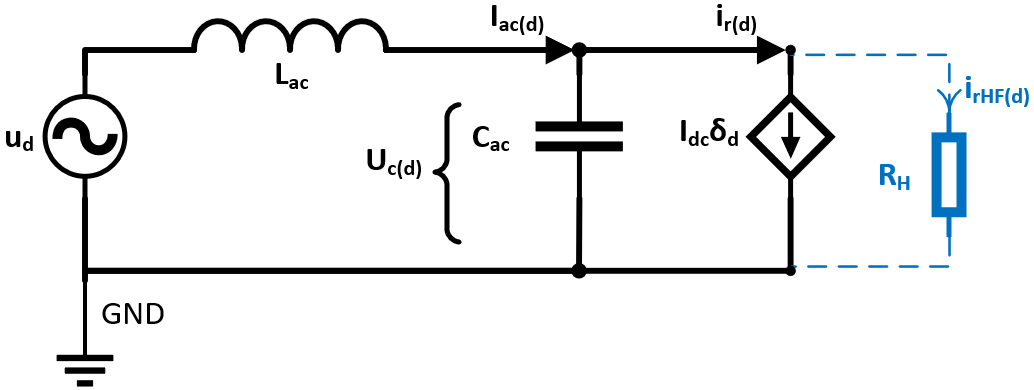
\includegraphics[width=\textwidth]{EMPC_PNG_Pics/ACdamping.png}
                    \caption{\centering Circuit schematics of AC damping.}
                    \label{EMPC:fig:ACdamping_a}
                \end{subfigure}
                ~ %add desired spacing between images, e. g. ~, \quad, \qquad, \hfill etc.
                  %(or a blank line to force the subfigure onto a new line)
                \begin{subfigure}[b]{.6\textwidth}
                    \includegraphics[width=\textwidth]{EMPC_PNG_Pics/ACchart.png}
                    \caption{\centering Control schematics of AC damping.}
                    \label{EMPC:fig:ACdamping_b}
                \end{subfigure}
                \caption{Circuit, and control schematics of AC damping via virtual damping resistance $R_H$, and high pass filter $HF(s)$.}
                \label{EMPC:fig:ACdamping}
            \end{figure}

     The resonance of the AC side LC filter produces harmonics in the capacitor voltage with frequency close to $\omega_{ac}=\frac{1}{\sqrt{L_{ac}C_{ac}}}$, which appears as $\omega_{ac}-\omega$ component in $u_{c_d}$, where $\omega=2\pi f$. The fundamental component of the capacitor voltage represents a DC component in the synchronous reference frame. Therefore, a high-pass filter (HF) is applied to filter out this DC component, with the transfer function:

    \begin{equation}
        \begin{array}{rcl}
            HF(s)&=&\frac{s}{s+0.1\cdot(\omega_{ac}-\omega)}.\\
        \end{array}
        \label{EMPC:equ:AC_HPF}
    \end{equation}

    \hlc[PT]{Adding the HF's transfer function and the virtual resistance, the damped dynamics follows:}

    \begin{equation}
    \hlcmath{PT}{
        \begin{array}{rcl}
        u_{c_d}&=&\frac{u_d}{s^2L_{ac}C_{ac}+1}-\frac{sL_{ac}I_{dc}\delta_d}{s^2L_{ac}C_{ac}+1}-\frac{HF(s)}{sC_{ac}R_H},\\
        \end{array}}
        \label{EMPC:equ:reduced_ucd}
    \end{equation}


    A virtual damping resistance $R_H$ has been defined for calculation of the damping current component $i_{rHF}$ from the HF component of the capacitor voltage, which can be observed in Fig. \ref{EMPC:fig:ControlStruct}, as well as in Fig. \ref{EMPC:fig:MPCStructure}.

\subsection{Modulation}\label{EMPC:sec:Modulation}

    \hlc[PT]{Modulation is required to govern the CSR device's switching states to realize the control displayed at} \ref{EMPC:fig:ControlStruct}. \hlc[PT]{In other words the reference current in Clarke frame $i_{r_{\alpha\beta}}$ needs to be translated into interpretable switching states for the device. In this work this is realised via space vector modulation (SVM), meaning that the current reference is converted to the superposition of the finite set of switching states the converter could realize without malfunction (some states are prohibited e.g. breaking the choke inductor's current flow.) Of course there are other modulation schools for example SHE (mentioned in section} \oldref{BASICCSR:sec:CSR_Literature}\hlc[PT]{) but they can not translate the control action so easily as SVM. As such they are not in the scope of the thesis.}\\
     The chosen modulation strategy is developed in the $"\alpha\beta"$ stationary reference frame, \hlc[PT]{where $i_{r_{\alpha\beta}}=\vec{i}_{ref}$}. Based on the notions already mentioned in section \oldref{BASICCSR:sec:OperationPrinciple}. The structure requires simultaneous conduction of the upper and lower transistors of the bridge, since the current of the $L_{dc}$  choke must not be interrupted. Additionally, the switching devices are considered as ideal.

    \begin{figure}[!ht]
        \centering
        \includegraphics[width=.6\textwidth]{EMPC_PNG_Pics/VectorPhasor.png}
        \caption{The fundamental input current vectors corresponding to the active switching states of the CSR.}
        \label{EMPC:fig:VectorPhasor}
    \end{figure}

    According to this, one of the upper and one of the lower switches must be closed at all times. This allows nine states, six of which are active. There are three "zero" vectors, corresponding to the switching states, when both devices of one of the bridge legs are in conduction. These current vectors are shown in Table \ref{EMPC:tbl:fundamental_vect}.


% Please add the following required packages to your document preamble:
% \usepackage{multirow}
% \usepackage[table,xcdraw]{xcolor}
% If you use beamer only pass "xcolor=table" option, i.e. \documentclass[xcolor=table]{beamer}

\begin{table}[]
\caption{The fundamental input current vectors corresponding to the active switching states of the CSR.}
    \begin{tabular}{|l|l|l|l|l|l|l|l|l|l|l|}
    \hline
    \rowcolor[HTML]{EFEFEF}
    \multicolumn{1}{|c|}{\cellcolor[HTML]{EFEFEF}}                                & \multicolumn{6}{c|}{\cellcolor[HTML]{EFEFEF}\textbf{Switching State}}       & \multicolumn{3}{l|}{\cellcolor[HTML]{EFEFEF}\textbf{Phase currents}} & \multicolumn{1}{c|}{\cellcolor[HTML]{EFEFEF}}                                                 \\ \cline{2-10}
    \rowcolor[HTML]{EFEFEF}
    \multicolumn{1}{|c|}{\multirow{-2}{*}{\cellcolor[HTML]{EFEFEF}\textbf{Name}}} & \textbf{1} & \textbf{2} & \textbf{3} & \textbf{4} & \textbf{5} & \textbf{6} & \textbf{ia}           & \textbf{ib}           & \textbf{ic}          & \multicolumn{1}{c|}{\multirow{-2}{*}{\cellcolor[HTML]{EFEFEF}\textbf{Vector representation}}} \\ \hline
    $\vec{i}_1$                                                                           & 1          & 0          & 0          & 0          & 0          & 1          & $i_{dc}$                   & 0                     & -$i_{dc}$                 & $2i_{dc}e^{j\pi/6}/\sqrt{3}$                                                                                           \\ \hline
    $\vec{i}_2$                                                                            & 0          & 0          & 1          & 0          & 0          & 1          & 0                     & $i_{dc}$                   & -$i_{dc}$                 & $2i_{dc}e^{j\pi/2}/\sqrt{3}$                                                                                           \\ \hline
    $\vec{i}_3$                                                                            & 0          & 1          & 1          & 0          & 0          & 0          & -$i_{dc}$                  & $i_{dc}$                   & 0                    & $2i_{dc}e^{j5\pi/6}/\sqrt{3}$                                                                                          \\ \hline
    $\vec{i}_4$                                                                            & 0          & 1          & 0          & 0          & 1          & 0          & -$i_{dc}$                  & 0                     & $i_{dc}$                  & $2i_{dc}e^{j7\pi/6}/\sqrt{3}$                                                                                          \\ \hline
    $\vec{i}_5$                                                                           & 0          & 0          & 0          & 1          & 1          & 0          & 0                     & -$i_{dc}$                  & $i_{dc}$                  & $2i_{dc}e^{j3\pi/2}/\sqrt{3}$                                                                                           \\ \hline
    $\vec{i}_6$                                                                            & 1          & 0          & 0          & 1          & 0          & 0          & $i_{dc}$                   & -$i_{dc}$                  & 0                    & $2i_{dc}e^{j11\pi/6}/\sqrt{3}$                                                                                           \\ \hline
    $\vec{i}_7$                                                                            & 1          & 1          & 0          & 0          & 0          & 0          & 0                     & 0                     & 0                    & 0                                                                                             \\ \hline
    $\vec{i}_8$                                                                            & 0          & 0          & 1          & 1          & 0          & 0          & 0                     & 0                     & 0                    & 0                                                                                             \\ \hline
    $\vec{i}_9$                                                                            & 0          & 0          & 0          & 0          & 1          & 1          & 0                     & 0                     & 0                    & 0                                                                                             \\ \hline
    \end{tabular}
        \label{EMPC:tbl:fundamental_vect}

\end{table}

    The neighboring space phasors can be formulated as:

    \begin{equation}
        \begin{array}{rcl}
            \vec{i}_n&=&\frac{2}{\sqrt{3}}i_{dc}e^{j(\frac{n\pi}{3}-\frac{\pi}{6})}\\
            \vec{i}_{n+1}&=&\frac{2}{\sqrt{3}}i_{dc}e^{j(\frac{n\pi}{3}+\frac{\pi}{6})}\\
            n&=&1,2,\dots,6,
        \end{array}
        \label{EMPC:equ:neighbor}
    \end{equation}

    which can be observed in Figure \ref{EMPC:fig:OnePhasor}.

    \begin{figure}[!h]
        \centering
        \includegraphics[width=0.6\textwidth]{EMPC_PNG_Pics/OnePhasor.png}
        \caption{Synthesis of $\protect\overrightarrow{i_{ref}}$ by $\protect\overrightarrow{i_{1}}$, $\protect\overrightarrow{i_{2}}$, and $\protect\overrightarrow{i_{0}}$}
        \label{EMPC:fig:OnePhasor}
    \end{figure}

    The reference current vector is sampled with fixed sampling period $T_s$. The sampled value of $\overrightarrow{i_{ref}}$ is synthesized as the time average of two neighbouring space phasors adjacent to the reference current:

    \begin{equation}
        \begin{array}{rcl}
            T_n\vec{i}_n+T_{n+1}\vec{i}_{n+1}&=&T_s\vec{i}_{ref}
        \end{array}
        \label{EMPC:equ:i_ref}
    \end{equation}

    $T_n$ and $T_{n+1}$ represent the individual durations of the switching states corresponding to the neighboring vectors. For example, in case of a current reference vector situated in the first sector, $T_1$, $T_2$ and $T_0$ can be calculated using \ref{EMPC:equ:dwelltime}.

    \begin{equation}
        \begin{array}{rcl}
            T_1&=&T_s\frac{i_{ref_\alpha}}{i_{dc}}\\
            T_2&=&T_s\frac{\sqrt{3}}{2i_{dc}}(i_{ref_\beta}-\frac{i_{ref_\alpha}}{\sqrt{3}})\\
            t_0&=&T_s-T_n-T_{n-1}=T_{7,8,9}
        \end{array}
        \label{EMPC:equ:dwelltime}
    \end{equation}

    The complex plane is naturally divided by the fundamental space vectors into six areas, named "sectors".

    \begin{equation}
        \begin{array}{l}
            x\frac{\pi}{6}+\frac{(n-1)\pi}{3}\leq\theta_n\leq\frac{\pi}{6}+\frac{n\pi}{3}\\
            n=1,2,\dots,6
        \end{array}
        \label{EMPC:equ:angle}
    \end{equation}

    The non-zero space vectors are selected based on the phase angle $\theta$ between $\overrightarrow{i_{ref}}$ and the real axis.
    Table \ref{EMPC:tbl:sequence} presents an example of switching pattern in case of a current reference vector situated in Sector I.\\
    The switching scheme represented in Table \ref{EMPC:tbl:fundamental_vect}. is aimed at reducing the number of commutations in a switching cycle, resulting in the reduction of the switching losses \cite{moussaoui2005open}.\\

    \begin{table}[h]
		\caption{Representation of switching sequences for SECTOR I.}
		\centering
        \includegraphics[width=0.8\textwidth]{EMPC_PNG_Pics/Sequence.png}
        \label{EMPC:tbl:sequence}
    \end{table}


    \hlc[PT]{Additionally, the implemented modulation logic prevents the reference from applying currents outside the modulation circle of} \ref{EMPC:fig:VectorPhasor}. \hlc[PT]{This is realised in} (\ref{EMPC:equ:refconstraint}) \hlc[PT]{resulting from the available magnitudes of the current vectors, is applied to the current reference, on top of the controller constraints in} \ref{EMPC:equ:numeric_constraints}.

    \begin{equation}
        \begin{array}{l}
            0\leq|i_{ref}|\leq\frac{\sqrt{6}i_{dc}}{cos\theta+\sqrt{3}sin\theta}
        \end{array}
        \label{EMPC:equ:refconstraint}
    \end{equation}

    \hlc[PT]{The modulation formulation is only meant to apply on the control action in the above mentioned ways (realizing and constraining the reference) since the switching frequency $fpwm$ is chosen so high that the controller dynamics match with the SVM state switching frequency. As such no lag or under-sampling is assumed, and the system dynamics are already implicit in the controller design.}


\subsection{Discussion}\label{EMPC:sec:Discussion}

    From the continuous AC \ref{EMPC:equ:mtx_AC}, and DC \ref{EMPC:equ:mtx_DC} model equations described in Ch.X., the controller is formulated form discretised system \ref{EMPC:equ:DiscreteStateSpace}, and it is described via the cost function and control problem of \ref{EMPC:equ:optim_problem}, and \ref{EMPC:equ:optim_problem_constr} in Ch.X$+$1. The evaluated model and control structure are shown on Fig.4. In the following section said EMPC’s computational requirements are evaluated, and the Matlab/Simulink simulation results are compared to a classic state feedback controller’s dynamic performance.

    \subsubsection{Lyapunov stability}\label{EMPC:sec:LyapStab}

    \hlc[PT]{The systematic finding of Lyapunov functions is described in detail in section} \oldref{BASICCSR:sec:MPCStability} \hlc[PT]{as well as in} \cite{borrelli2017predictive}. \hlc[PT]{The explicit receding horizon control law formulated in section} \oldref{EMPC:sec:DCside} \hlc[PT]{is mapped according to} \ref{EMPC:equ:quadratic_set}, \hlc[PT]{resulting the partitioning of the constrained state space displayed on Fig.} \ref{EMPC:fig:regions}.\hlc[PT]{ Considering system} \ref{EMPC:equ:DiscreteStateSpace} \hlc[PT]{with the given constraints of} \ref{EMPC:equ:numeric_constraints} and RHC law \ref{EMPC:equ:optim_problem}, \hlc[PT]{the assumption is that a maximal positive-, and control invariant set $\mathcal{X}_f$ can be obtained for the closed loop system, for every defined critical region. For finding and $\mathcal{X}_f$ and the feasibility of constructing the critical region specific Lyapunov function an implemented verification method is available from} \cite{MPT3}, \hlc[PT]{by searching $\mathcal{X}_f$ for the closed loop autonomous PWA system. Then piece-wise quadratic (PWQ) Lyapunov function can be constructed displayed on Fig} \ref{EMPC:fig:LyapStab}.

    \begin{figure}[!h]
        \centering
        \includegraphics[width=\textwidth]{EMPC_PNG_Pics/LyapunovPatrition_trans.png}
        \caption{Lyapunov function for EMPC every partition.}
        \label{EMPC:fig:LyapStab}
    \end{figure}


    \subsubsection{Computational effort}\label{EMPC:sec:CompEffort}

    The binary search tree generated for the control problem presented in Fig. \ref{EMPC:fig:SearchTree}. The search method and formulation of the tree is described in chapter \ref{BASICCSR:sec:EMPCStorage}. The depth of the search tree is 5 and it has a total number of 29 nodes. It is utilized with the MPT toolbox \cite{MPT3}, and it can be used for the computationally optimal real-time implementation of the proposed algorithm on low-cost hardware.

    \begin{figure}[!ht]
        \centering
        \includegraphics[width=\textwidth]{EMPC_PNG_Pics/SearchTree.png}
        \caption{Binary search tree of the controller for a horizon of $N = 4$. The leaf nodes are depicted with filled squares. The depth of the tree is 5.}
        \label{EMPC:fig:SearchTree}
    \end{figure}

    The search for an active critical region starts from the first level and represents the evaluation in each adjacent node of an inequality of the form: $x\leq K$. Thus, in this case a maximum number of 4 inequalities have to be evaluated to reach the active critical region. Implementing the presented algorithm is straightforward on a DSP processor, for instance from the dsPIC33 family by Microchip. Using the MAC (multiply and accumulate) instruction the inequality is evaluated for each node using 4 instructions, thus in 80 ns on a 50 MIPS processor (Fig. \ref{EMPC:fig:Memory}). The active critical region can be reached in a maximum of 400 ns. Compared to the typical sample rate of 10us in the case of a CSR, the real-time implementation on a DSP processor is possible. More information about storing critical regions can be found in \oldref{BASICCSR:sec:EMPCStorage}.

    \begin{figure}[!ht]
        \centering
        \includegraphics[width=\textwidth]{EMPC_PNG_Pics/Memory.png}
        \caption{Data organization in the data memory of a single core DSP and the evaluation of a 2-dimensional inequality}
        \label{EMPC:fig:Memory}
    \end{figure}

    More information about storing critical regions can be found in \oldref{BASICCSR:sec:EMPCStorage}.

    \subsubsection{Horizon performance}\label{EMPC:sec:Performance}

    With the cost function \ref{EMPC:equ:optim_problem} employed using \ref{EMPC:equ:quadratic_mtx_set}, changing the length of the horizon $N$ affects the system's complexity illustrated by the partition in the state space shown in Fig. \ref{EMPC:fig:regions}, and Fig. \ref{EMPC:fig:MultiHorizon} presents the step response of the controlled system for different lengths of the horizon. \hlc[PT]{It shows, that the response is heavily affected by the horizon length at the first three iterations, rendering the one step choice useless, whilst by increasing the horizon, the steady state error of the algorithm decreases.}

    \begin{figure}
                \centering
                \begin{subfigure}[b]{\textwidth}
                    \includegraphics[width=\textwidth]{EMPC_PNG_Pics/MultiHorizon2_trans.png}
                    \caption{\centering Overall performance of the EMPC, with different control horizons.}
                    \label{EMPC:fig:MultiHorizon_a}
                \end{subfigure}
                ~ %add desired spacing between images, e. g. ~, \quad, \qquad, \hfill etc.
                  %(or a blank line to force the subfigure onto a new line)
                \begin{subfigure}[b]{\textwidth}
                    \includegraphics[width=\textwidth]{EMPC_PNG_Pics/HorizonPerformace_trans.png}
                    \caption{\centering The projection on the time axis indicates the decrease of steady state error with the horizon length.}
                    \label{EMPC:fig:MultiHorizon_b}
                \end{subfigure}
                \caption{Step response of the system as a function of the horizon length $N$.}\label{EMPC:fig:MultiHorizon}
            \end{figure}

    \hlc[PT]{Unfortunately, the steady state error is is still present after the computational boundary of \textbf{XY} ns regardless of increasing the horizon. As such an additional integrator component is advised to embed into the model equations of} \ref{EMPC:equ:mtx_DC}\hlc[PT]{, aka. augment the model, and The results can be observed in the next section and on Fig.} \ref{EMPC:fig:Regions_augment}.

    \subsubsection{Simulation results}\label{EMPC:sec:Results}

    The simulation results are produced with Matlab/Simulik. The discrete model's \ref{EMPC:equ:DiscreteStateSpace} simulation frequency was 1 MHz, with the model parameters represented in Table \ref{EMPC:tbl:params}. \hlc[PT]{As mentioned the base control structure has considerable steady state error, which can be mitigated, by increasing the control horizon, but the computation cost is NP-heavy. The solution is to augment the model with an additional integrator. As such, with some re-parametrisation with the const function weights:}

     \begin{equation}
    \hlcmath{PT}{
        \begin{array}{l}
            \textbf{R}_w=\begin{bmatrix}
                1\cdot10^{-6}\\
            \end{bmatrix},
            \textbf{Q}_w=\begin{bmatrix}
                1& 0\\
                0& 1\\
            \end{bmatrix},
            N=4,
        \end{array}}
        \label{EMPC:equ:quadratic_mtx_set}
    \end{equation}

    \hlc[PT]{the partition space grows to 49 regions but the steady state error lessens significantly. The comparison of the EMPC performances is shown on Fig. }\ref{EMPC:fig:Result_PerformanceEMPC}.

%    \begin{figure}[!ht]
%        \centering
%        \includegraphics[width=\textwidth]{EMPC_PNG_Pics/Result_3fEMPC.png}
%        \caption{Three-phase voltage and current intake of the CSR with EMPC}
%        \label{EMPC:fig:Result_3fEMPC}
%    \end{figure}

    \begin{figure}[!ht]
        \centering
        \includegraphics[width=\textwidth]{EMPC_PNG_Pics/Results.png}
        \caption{Resulting current and voltage trajectories of the CSR with (EMPC).}
        \label{EMPC:fig:Result_PerformanceEMPC}
    \end{figure}

    More details about the Matlab simulation are presented in \cite{neukirchner2019linkedmodel}.

    \subsubsection{Comparison with a state feedback control}\label{EMPC:sec:Comparison}

    On the DC side, not only the output voltage $u_0$ but also the inductor current $i_{dc}$ needs to be controlled. Described in \cite{zhang2015simplified}, a state feedback control with optimal parameters can be used as a reference based on the model properties listed in Table \ref{EMPC:tbl:params}, with output voltage $u_0$ and DC bus current $i_{dc}$ chosen as the state variables. Since $u_0$ is a DC quantity in steady state, an integrator signal is introduced to diminish the steady-state error. The structure of the controller is represented in Fig. \ref{EMPC:fig:SFeedbackDC}.

    \begin{figure}[!ht]
        \centering
        \includegraphics[width=0.7\textwidth]{EMPC_PNG_Pics/SFchart.png}
        \caption{Simple DC side state feedback control structure.}
        \label{EMPC:fig:SFeedbackDC}
    \end{figure}

    The tuning constants applied and calculated according to \cite{godlewska2015predictive} are:

    \begin{equation}
    \hlcmath{PT}{
        \begin{array}{l}
            k1=\frac{\omega^3_n}{1.5U_n\omega^2_{dc}},\,k2=\frac{2.2\omega^2_n}{1.5U_n(\omega^2_{dc}-1)},k3=\frac{1.9\omega_n L_{dc}}{1.5U_n},\,\\
        \end{array}}
        \label{EMPC:equ:tuning}
    \end{equation}

    where $\omega_n=1.1,\,\omega_{ac}=\frac{1}{\sqrt{L_{ac}C_{ac}}},\,\omega_{dc}=\frac{1}{\sqrt{L_{dc}C_{dc}}}$. The state feedback controllers block on the diagram is taking the controller's place, shown on Fig. \ref{EMPC:fig:ControlStruct}. The independent outputs are the high pass filter's output  $i_{rHF(d)}$ and the controller's output $i_{ref}=i_{rcontrol(d)}$. The sum of the independent current values is converted to Clarke frame to be able to govern the switching states of the IGBT's. This can be done because $i_{rHF(d)}$ has only high frequency components and $i_{rcontrol(d)}$ has low frequency components due to the differences in LC time constants, as discussed in the second section. Then the control signal governing the switches is applied in the same manner, described at the start of section \oldref{EMPC:sec:Modulation}.
    The state feedback control's performance in comparison with the EMPC is shown in Fig. \ref{EMPC:fig:Result_EMPCfinal}.

    \begin{figure}[!ht]
        \centering
        \includegraphics[width=\textwidth]{EMPC_PNG_Pics/Compare.png}
        \caption{Resulting current and voltage trajectories of the CSR with explicit model predictive control (MPC) compared to the $N=10$ case (MPCN10), the augemnted model (MPCAUG), and the state feedback control (SF).}
        \label{EMPC:fig:Result_EMPCfinal}
    \end{figure}

\section{Conclusion}\label{EMPC:sec:Conclusions}

    The constrained, model-based optimal control of a current source rectifier has been presented in this dissertation. The dynamic model of a three-phase current source rectifier has been developed in Park frame. The proposed model has been examined from the design and implementation points of view with the purpose of explicit model-based predictive control. It proved to be the case that the regular set of differential equations of the CSR appears to be too complex, and contains non-linearity for such a design approach. To address this issue the usage of separated AC and DC equation sets was suggested to avoid linearization and complexity reduction. This solution eliminates bilinearity and enables the application of linear control design techniques. Current-based SVPWM of the three-phase converter has been used with an emphasis on the reduction of switching losses. Throughout the chapter the explicit model predictive control method is described and the method's effectiveness compared to conventional state feedback control is show. The implementation and simulation experiments have been performed in Matlab/Simulink environment. Moreover, the proper implementation of the system in a modern DSP chip will result in real-time operation. 
\newpage
\section{Notations used in the chapter}
		
		%\begin{longtable}{r|l}
  % after \\: \hline or \cline{col1-col2} \cline{col3-col4} ...
  %Chapter 4.1. notations&\\
  \begin{scriptsize}
\begin{tabularx}{\textwidth}{r|X}
  
  %%A
  $\textbf{A}$                  & State matrix of the DC side system\\
  $\textbf{A}_d$                & Discretised state matrix of the DC side system\\
  $\textbf{A}_x$              & Constraint state matrix\\
  $\textbf{A}_u$              & Constraint input matrix\\
  $\textbf{A}_f$              & Constraint state matrix at the end of the horizon\\
  $\mathcal{A}$               & Set if indices in states where the constraints are active\\
  $\mathcal{A}^N$               & Set if indices in states where the constraints are inactive\\
  
  %%B
  $\textbf{B}$                  & Input matrix of the DC side system\\
  $\textbf{B_d}$                & Discretised input matrix of the DC side system\\
  
  %%C
  $C_{ac}$                          & AC side inductance\\
  $C_{dc}$                          & DC side inductance\\
  $\textbf{C}$                  & Output matrix of the DC side system\\
  $\textbf{C_d}$                & Discretised output matrix of the DC side system\\
  $C_{reg_i}$                       & Critical region\\
  
  %%D
  $D(-\Theta)$                      & Inverse Clarke transformation\\
  
  %%E
  $\textbf{E}$                & Unified constraint state matrix \\
  
  %%F
  $\textbf{F}$                & State coefficient matrix for calculating the optimal input \\
  $f$                               & Network voltage frequeny\\
  $fpwm$                            & Rectifier switching frequency\\
  $f_s$                             & Simulation frequency\\
  $f_i$                             & Function of state at the $i^th$ step\\
  
  %%G
  $\textbf{G}$                & Unified constraint input matrix \\
  $g_i$                             & Function of input at the $i^th$ step\\
  
  %%H
  $H$                               & Supplementary quadratic optimizer matrix\\
  $HPF(s)$                          & High pass filter transfer function\\
  
  %I
  $i_{abc}$                         & Generic three phase current\\
  $i_{ac_{1,2,3}}$                  & AC side inductance current\\
  $i_{ac_{\alpha,\beta}}$           & AC side inductance current in Clarke frame\\
  $i_{ac_{d,q}}$                    & AC side inductance current in Park frame\\
  $i_{HPF}$                         & AC side damping current\\
  $i_{r_{1,2,3}}$                   & Rectifier current\\
  $i_{rMPC_d}$                      & Direct component of the output of the EMPC controller\\
  $i^*_{r_{1,2,3}}$                 & Rectifier reference current\\
  $i^*_{r_{\alpha,\beta}}$          & Rectifier reference current in Clarke frame\\
  $i_{rcontrol_d}$                  & Direct component of the output of the DC voltage controller\\
  $i_{rHF_d}$                       & Direct component of the damping current of AC noise\\
  $i_{dc}$                          & DC side inductance current\\
  $i_{ref_{\alpha,\beta,\gamma}}$   & $\alpha$, $\beta$, or $\gamma$ component of the reference current vector respecively\\
  $i_{dq0}$                         & Three phase current converted to Park frame\\
  $\vec{i}_{0,\dots,9}$             & Current vector of the phasor\\
  $\vec{i}_{ref}$                   & Reference current vector\\
  
  %%J
  $\mathcal{J}$                     & Set if indices of active constraints\\
  $J$                               & Quadratic EMPC cost function\\
  $J^*$                             & Optimal cost value\\
  $J_0$                             & Cost function to optimize at the initial state\\
  $J^*_0$                           & Optimal cost function at the initial state\\
  
  %%K
  $\mathcal{K}$                     & Set of controller gains respective to critical regions\\
  $K$                               & Feedback gain of EMPC controller\\
  $k_{1,2,3}$                       & State feedback controller's coefficients\\
  
  %L
  $L_{ac}$                          & AC side inductance\\
  $L_{dc}$                          & DC side inductance\\
  $L_S$															& Input filter inductance of the three phase alternating current in VSR\\
  $L_D$															& Inductor for filtering the output current of the CSR (Choke)\\
  
  %%N
  $N$                               & Control horizon\\
  $N_y,N_u,N_c$                     & Output, input and constraint horizons\\
  $n$                               & Current phasor sector indicator\\
  
  %%P
  $\mathcal{P}^c$               & Set of all (input and state) constraints at time instance\\
  $\mathcal{P}_p$             & Set of primary feasibility conditions\\
  $\mathcal{P}_d$             & Set of dual feasibility conditions\\
  $P_n$                             & Nominal power of the CRS\\
  $\textbf{P}$                    & Terminal penalising weight matrix\\
  $\textbf{P}_N$                    & Terminal penalising weight matrix at the end of the horizon\\
  
  %%Q
  $\textbf{Q}$                & State weight matrix of quadratic MPC cost function\\
    $\bar{\textbf{Q}}$                    & Batch of state penalising weight matrix\\
  
  %%R
  $R$                               & Phase resistance\\
  $R_H$                             & Virtual damping resistance\\
  $R_{load}$                        & Load resistance\\
  $\textbf{R}$                & Input weight matrix of quadratic MPC cost function\\
  $\bar{\textbf{R}}$                    & Batch of input penalising weight matrix\\
  $\mathbb{R}$                      & Set of real numbers\\
  
  %%S
  $S$                               & Current phasor sector\\
  $\textbf{S}$                  & Coefficient constraint matrix\\
  $\mathcal{S}^x$             & Set of all possible future state matrices stepping through the horizon\\
  $\mathcal{S}^u$             & Set of all possible future input matrices stepping through the horizon\\
  
  %%T
  $T_s$                             & Switching period\\
  $T_{0,\dots,9}$                   & Dwell time in the corresponding sector\\
  $t$                               & Discrete timestep\\
  
  %%U
  $U$                               & Set of MPC inputs\\
  $Un$                              & Network line-to-line voltage\\
  $\textbf{U}^*_0$            & Optimal vector of future inputs starting from the initial state\\
  $\mathcal{U}^u$             & Set of inputs not violating constraints\\
  $\textbf{u}^*$                & Optimal vector of input\\
  $\widehat{u}$				 & Peak value of AC-side capacitor voltage\\
  $\textbf{u}$                  & Output vector of the DC side system\\
  $u_{1,2,3}$                       & AC side phase voltage\\
  $u_{\alpha,\beta}$                & AC side phase voltage in Clarke frame\\
  $u_{d,q}$                         & AC side phase voltage in Park frame\\
  $u_{c_{1,2,3}}$                   & AC side capacitance voltage\\
  $u_{c_{\alpha,\beta}}$            & AC side capacitance voltage in Clarke frame\\
  $u_{c_{d,q}}$                     & AC side capacitance voltage in Park frame\\
  $u_0$                             & DC side voltage on load\\
  $u^*_0$                           & DC side voltage reference\\
  $u_{MPC}$                         & MPC control variable\\
  $\textbf{u}^*$                & Optimal input vector\\
  
  %%V
  $v_D$								& Output voltage before the choke inductor $L_D$\\
  $v_{i,j}$							& Three phase phase-to-neutral voltage $i,j\in\{R,S,T\}$\\
  $v_{N,RS}$						& Three phase line-to-line voltage of $R$ and $S$\\
  $v_{c_p}$							& AC-side capacitor voltage, where $p\in\{1,2,3\}$\\
  $\hat{v}$							& Voltage peak\\
  
  %%W
  $\textbf{w}$                & Unified constraint vector \\
  
  %%X
  $\mathcal{X}^x$             & Set of all possible future states stepping through the horizon\\
  $\mathcal{X}_f$             & Set of all possible future states at the end of the horizon\\
  $\mathcal{X}_0$             & Set of initial states\\
  $\textbf{x}$											& State vector of a linear time invariant model\\
  $\bar{\textbf{x}}$											& Minimum state value of the objective function\\
  $\textbf{x}(0)$                 & Initial state\\
  
  %%Y
  $\textbf{y}$                  & Input vector of the DC side system\\
  $\textbf{Y}$                  & Remainder supplementary matrix\\
  
  %%Z
  $\textbf{z}$                  & Vector of optimization variables\\
  $\textbf{Z}^*$              & Set of optimizers leading to feasible states\\
  $\textbf{z}$											& Optimizer of linear multi parametric problem\\
  $\tilde{\textbf{z}}$        & Set of all future states and inputs over the horizon\\
  
  %%Greek
  $\delta_{1,2,3}$                  & Conduction state leg\\
  $\delta_{\alpha,\beta}$           & Conduction state leg in Clarke frame\\
  $\delta_{d,q}$                    & Conduction state leg in Park frame\\
  $\theta$                          & Network voltage vector’s angular displacement\\
  $\epsilon,\varphi,\chi,\psi$               & Constant sets\\
  $\Omega$                          & Closed and bounded set of states containing the origin\\
  $\omega$                          & Network voltage vector’s angular velocity\\
  $\omega_{ac}$                     & Ac side LC filter angular velocity\\
  $\omega_{n}$                      & Damping angular velocity\\
  \end{tabularx}
  \end{scriptsize} 

% Summary
\chapter{Thesis and Summary}

\section{Summary}

The topic of this PhD. dissertation is optimal current control. The aim of the research was to apply and simulate high frequency controllers with optimization purpose of cost functions with the presence of constraints and circumstances, on controlled switch based power electronic devices.\\
In chapter \oldref{VUB:sec:Main}, a current controlled inverter structure was presented, connected to a small, domestic grid, representing the connection of a household with possible renewable (or other) generators, to balance consumption. The examined grid, the phenomena of voltage unbalance was assumed to be present, as the main problem, of which this device was ought to not only handle, but mitigate within the limit of its physical capabilities. For this reason, first an indicator was established, based on a proposed geometrical operation, as a voltage unbalance norm candidate (section \oldref{VUB:sec:Geom}). This norm was calculated from the symmetrical difference between the convex hull of voltage phasor vectors, always present on a three phase network. The idea was, that any deviation from the ideal phasor, (which first vector assumed in phase with the ideal one) introduces sub-optimal behavior, or fault of appliances connected. This way the already present indicators of voltage unbalance was examined (section \oldref{VUB:sec:AdditionalContent}). Afterwards found that not only, they vary in result, but ignore phase differences, or the zero-sequence component (based on the Fortescue method), or its ponderous to serve as a cost function need to be minimize. The proposed geometrical norm however considers all of the above, with the addition that since it calculates area, instead of vector length differences, the result is a square-like function, serves as an excellent candidate. The downside is the yet unresolved computational overload, that is method introduces.\\
In the next phase, the network's unbalance was attempted to be mitigated by designing a power electronic converter for a household, which utilizes an external power source (a photo voltaic source in this case) for counter balance (section \oldref{VUB:sec:Compensation}). This way some obstacles needed to be dealt with, first and foremost, the highly stochastic nature of the network. It was assumed, that the device has no external information, rather than the voltage, measured at the network connection point. This way a non-model based asynchronous parallel pattern search (APPS) controller was designed and applied based on the said geometrical norm, which decreases the cost regardless of unknown circumstances. Furthermore, the device needed various subunits, to efficiently handle the power flow in all three phases, namely power-point-tracking, intermediate voltage control, and per-phase current injection was required. The results were tested in Matlab/Simulink environment with simulating the actual device via Simscape, and the unbalanced network, also with experimental measurements. The result was, that the controller could reduce the network's voltage unbalance, based on the network's robustness (how large is the impedance, which created the unbalance), how much control reserve is present as energy source, and physical boundaries (the device can not supply infinite current). Based on this the household's normal operation can withheld even in with unbalanced loads.\\
Lastly in chapter \oldref{EMPC:sec:main} in-depth modeling and predictive control task has been performed, on one power electric component, namely on a buck-type rectifier. This rectifier uses current source operation to supply the load it is connected to. The main goal was to create on the Kirchhoff's law based differential equations a model based predictive controller, suited to reach the reference point with the best dynamics. It was also taken in mind, that an implicit MPC would not be up to the task, sice every control rule was to be re-calculated from scratch, implying a very expensive CPU. This gap could be bridged by reaching out for the explicit MPC method, by partitioning the state space, on a pre-defined rule set. This way the control demand could be reduced significantly, however, this is not suited for high rank systems. As such the system's bi-linearity was eliminated by applying on the premise that two dynamics which have highly different fundamental frequencies can operate in superposition. This way the problem was simplified, and explicit MPC could be implemented in DC-side, whilst active damping at the AC-side. The method's efficiency was tested in Matlab/Simulink environment against a conventional state-feedback controller, with good results. Additionally the computational demand was evaluated, with assumed binary search algorithm.\\

\section{New scientific results}

\begin{enumerate}[I.)]

\item\textbf{Thesis}: \emph{Geometrical indicator for voltage unbalance in three phase networks}\\
    \textbf{Related publications:} \cite{neukirchner2015examination}, \cite{Neukirchner2015}.\\
    I extended the currently used measures of voltage unbalance with a new norm candidate. I found out that it is more demanding from the computational point of view, but has a new feature namely it checks electrical asymmetry, i.e. the norm of a $\pm120$ degree rotated version of the ideal three phase phasor is zero in the geometrical sense. I compared my geometrical approach to the standard wide-spread use of voltage unbalance factor (VUF) and found out it carries additional information, whilst retaining it's original purpose.\\
		
\item\textbf{Thesis}: \emph{Voltage unbalance compensation with optimization based control algorithm and asymmetrical inverter structure}\\
    \textbf{Related publications:} \cite{Neukirchner2015}, \cite{neukirchner2016voltage}, \cite{neukirchner2017voltage}.\\
     I found out that the regular current controlling applications would not fit to the purpose for reducing voltage unbalance whilst only relying on the voltage measurement. As such I developed an asymmetrical current source inverter (ACSI) circuit with combined asynchronous parallel pattern search (APPS) control structure, in Matlab/Simulink environment, and I applied the my geometrical norm as a cost function. I showed with validating simulations, that the geometrical based unbalance indicator can serve as a basis of further research. \\
		The fundamental element of the system is a modified three phase inverter that is capable of the asymmetric injection of any current waveforms to the network. The optimization based control algorithm injects the available energy (as current waveform) in such a way, that the voltage unbalance decreases. The structure enables to show that any point the inverter is connected, could restore power quality with a certain degree such unbalance compensation. This optimization problem is usually constrained by the available renewable energy supplied by the power plant. This suggested controller with combined inverter structure enables the residential users owning a grid synchronized domestic power plant to reduce voltage unbalance measurable at any low voltage domestic the connection point. \\
    I also tested the control structure on a real low voltage network model in a dynamical simulation environment consisting of the models of the electrical grid, a domestic power plant, ACSI, and different types of loads. Different simulation experiments has been run for each norm and for both the power constrained and unconstrained case. I showed with the evaluation that this structure can serve as a residential level voltage quality improvement method for the three phase low voltage network.\\
		
		\item\textbf{Thesis}: \emph{Constrained, explicit predictive control for current source buck-type rectifiers}\\
        \textbf{Related publications:} \cite{neukirchner2020constrained}.\\
    I proposed a simplified CSR model, which was derived from the well known CSR structure and was examined from design and implementation points of view with the purpose of explicit model-based predictive control. The regular set of differential equations of the CSR appeared to be too complex for my a design approach, for applying explicit predictive control. \\
		I adressed this issue with the separation AC and DC equation sets was of the CSR to decrease complexity and easy controller design. With this solution I eliminated bi-linearity and enabled the application of linear control design techniques. I used current-based SVPWM the modulation, what has been used with an emphasis on the reduction of switching losses. \\
		For DC side control I implemented explicit model predictive control (EMPC) and I compared this method's effectiveness to conventional state feedback control. I implemented the CSR structure and the proposed controller with EMPC on DC and active damping on the AC side in Matlab/Simulink environment and tested by simulation. Additionally, I tested the proper implementation's computational requirements in a modern DSP chip, which would serve in real-time operation.\\
	
\end{enumerate}

Publications not related to the thesis:  \cite{neukirchner2011modeling}, \cite{neukirchner2014quasi}, \cite{gollei2014measurement}, \cite{neukirchner2016modelling}.


		\section{Applications and future work}
		
		In this section the possible applications shall be described based on my thesis. These are not yet scope of current research activities, but can serve as a potential direction and evolution for these results.
		
		\subsection{Geometrical voltage unbalance norm}
		
		As mentioned the geometrical norm's largest weakness is the computational demand. The required areas, computed from the voltage phasors realized with the corresponding Matlab functions, which are not designed for continuous calculation, especially not for time constants for power electronic devices. This can be resolved, via replacing the calculation of the symmetrical difference (difference between the two polygon's union and intersection) with finite-element method, with scalability, where the segmentation's resolution would be adjustable and based on the corresponding simulation's (or system's) time constant and the simulator machine's calculation capabilities. After this, the calculation method shall be phrased in an traditional equation form, using the toolset of set theory, and linear algebra. This way, the norm's calculation could be further reduced, and could be implemented on a cheaper embedded system.\\
		The geometrical norm's usefulness was already proven compared o the regular $VUF$ method. However the robustness of the method seems implicitly proven, is shall be tested on real conditions, even in extreme (faulty) situations, and with such hard constrains could be defined, where the algorithm outlives its usefulness. This way, instead of just a resulting number, a full formulation of an optimization problem could be utilized, presented in section \ref{BASICCSR:sec:OptimalControl}, with model based predictive capabilities. This can be further enhanced, with recognizing different scenarios, form general inefficiency, to fault prediction, or handling (like graceful degradation).
		
		\subsection{Voltage unbalance reducing inverter structure}
		
		The inverter structure employ a variety of subsystems, which shall work together in harmony. A global optimum shall be defined (with weighting the various factors) based on external circumstances, and the customers needs. This way, the individual Kirchhoff equations based differential equations shall be established, and controller designed.\\
		The APPS method, however fulfills its optimizing responsibilities very well in such an environment, where changes are expected to be highly stochastic, based on network knowledge, a network- and/or device model based optimal control shall be established, where various current and voltage inertias can be taken into account, giving a leverage for prediction.\\
        \hlc[KP]{The setup of the subsidiary network is is using a very basic network setup. The controller needs to be tested on real world low voltage network models with multiple topologies, and circumstances, established by other research groups and companies, to have a good representation of the system's capabilities.}\\
        \hlc[KP]{The total harmonic distortion (THD) was not in the scope of the research, as such, there was no counter measure implemented in the control cycle, to prevent increasing the system's THD. In an experimental setup this needs to be addressed.}\\
        \hlc[KP]{The controller is not handling reactive power well, means the reactive power evolution was not in the scope of the research, as such due to the unpredictable nature of the network, the injected reactive power could be an issue.}\\
        This way the system's physical properties shall be scalable (based on a household's needs and its energy producing and storing capabilities), as in designing a real power electric system for implementation. Next actual implementation shall be proceeded, with prototype realization on a test bench, with a simulated domestic network connection. Further step to test the presence of multiple of such devices on the network, and how they could mitigate unbalance in synchronous or asynchronous operation. \\
        
		
		\subsection{Explicit model predictive control for buck-type rectifier}
		
		From mathematical perspective it is an alternative possibility to take the harder route and take the inherent bilinearity into account. This way, the devices equations should not be partitioned, and a hybrid design can be commenced. This has been performed in the literature, but seldom on three phase systems, for complexity reasons.\\ The topology could be altered, by removing (or greatly decreasing) some of the device's filtering  capabilities, in inductive or capacitive terms (some inductors, like the choke $L_{dc}$ are non-removable), and try to outsource this problems to the controller itself to some degree.\\
		Try the cost function from Euclidean norm to an infinity norm, and also give stricter constrains. The optimum could be power throughput based instead of a specified current. The types of loads can be extended, and merged with the current equation system. This enables to expand the research on electric machinery, where starting/ breaking dynamics can be tested. On the other side, the effects on the supplying network can be taken into consideration, further reducing harmonics, and test conditions in the presence of unbalance.
		Lastly, experimental results shall be performed on a device, further validating its usefulness, and implement the used S-function from Simulink to an embedded system.
 %--> List of thesis and own publications moved here <=====

%% Appendix
\chapter*{Appendix}

\section{Network substitute model}\label{APPENDIX:sec:Network_substitute}

For the voltage unbalance compensation setup, a substitute network model was used, to be able to recreate said phenomena. The network is a very simplified version of a low voltage residual area with two symmetric loads, a symmetric ohmic load, and one asymmetrical load, for decreasing the voltage quality. See Figure \ref{fig:expnetwork} for details.

\begin{figure}[ht]
            \centering
            \includegraphics[width=0.95\textwidth]{Unblance_EPS_Pics/Network.png}
            \caption{Network model, for creating an environment for voltage unbalance compensation setup.}
            \label{fig:expnetwork}
            \end{figure}

The network has the following components:

\begin{itemize}
\item \textbf{Voltage measurement:} Either could be an ideal three phase sine wave or the measured voltage at the university laboratory. See section \oldref{VUB:sec:Measurement} for further details. The voltage values $V_a$, $V_b$, and $V_c$ are representing the measurable network voltage, and $R_s=0.4\Omega$ is representing the source resistance.
\item Line multiplexer: substitutes the three phase four wire connection with one representative line between the actors.
\item Network segment: Influences the network topology, and represents the line between actors. The network segment is modelled with $0.4\Omega$ wire resistance on each of the four lines. The network's power loss is measured in these line segments.
\item Symmetric Ohmic load: Symmetrical resistive component at the end of the main branch, with $50\Omega$ on each phase.
\item Three phase parallel RLC load: Represents an unbalance-neutral actor, with balanced RLC loads on each phase in star connection, where the load's active power is $\frac{10000}{3}W$, inductive reactive power is $\frac{2000}{3}VAr$, and the capacitive reactive power is $0VAr$.
\item Asymmetrical load: The load mainly responsible for the network unbalance. There loads connected to the phases are:
\begin{itemize}
    \item Active power: $5kW$, Inductive reactive power: $1kVAr$, Capacitive reactive power: $0.5kVAr$.
    \item Active power: $5kW$, Inductive reactive power: $0.555kVAr$, Capacitive reactive power: $0.111kVAr$.
    \item Active power: $5kW$, Inductive reactive power: $0.277kVAr$, Capacitive reactive power: $0.055kVAr$.
\end{itemize}
\item Unbalance compensator: The device responsible for decreasing the network unbalance. Setup and function was detailed in chapter \oldref{VUB:sec:Compensation}.
\end{itemize}       


\section{Geometric approach to multi parametric programming}\label{BASICCSR:sec:MPP}
    % Section's main text due to more comprehensible source

    In this section the goal is to explain how to solve multi-parametric optimization problems (mp-OP). By start lets consider the following linear multip-parametric problem:

        \begin{equation}
    \begin{array}{rcl}
            J^*(\textbf{x})&=&\min_{\textbf{z}}J(\textbf{x},\textbf{z})=\textbf{c}'\textbf{z}\\
            %&=&\frac{1}{2}\textbf{z}'\textbf{H}\textbf{z}\\
            &\textnormal{subj. to}&\textbf{Gz}\leq\textbf{w}+\textbf{Sx},
        \end{array}
        \label{BASICMPC:equ:MPP_program}
    \end{equation}

    where $\textbf{z}\in\mathbb{R}^s$ is the vector of the optimization variables,  $\textbf{x}\in\mathbb{R}^n$ is the vector of parameters, and of course $J(\textbf{x},\textbf{z}):\mathbb{R}^{s+n}\rightarrow\mathbb{R}$ is the objective or cost function. Additionally $\textbf{G}\in\mathbb{R}^{m\cdot s}$, $\textbf{w}\in\mathbb{R}^m$, $\textbf{c}\in\mathbb{R}^s$ and $\textbf{S}\in\mathbb{R}^{m\cdot n}$ as described in section \ref{BASICCSR:sec:OptimalControl}. Next we define a closed convex parameter set $\textbf{K}\subset\mathbb{R}^n$ such as:

    \begin{equation}
    \begin{array}{rcl}
            \textbf{K}&=&\left\{ \textbf{x}\in\mathbb{R}^n:\textbf{Tx}\leq\textbf{Z}\right\},
        \end{array}
        \label{BASICMPC:equ:MPP_parameterset}
    \end{equation}

    where $\textbf{K}^*\subseteq\textbf{K}$ is the set where \ref{BASICMPC:equ:MPP_program} is feasible, and $\textbf{x}^*\in\textbf{K}^*$ where $\textbf{x}^*$ is the optimum. It is further assumed that:

    \begin{enumerate}
    \item the constraint $\textbf{x}\in\textbf{K}$ is included in the constraints of $\textbf{Gz}\leq\textbf{w}+\textbf{Sx}$.
    \item $\textbf{K}$ is a full dimensional polytope, or the problem can be reformulated to $\textbf{K}$ to be full dimensional with a smaller set of parameters.
    \item $\textbf{S}$ is on full rank, or the problem can be reformulated to $\textbf{S}$ to be full rank with a smaller set of parameters.
    \end{enumerate}

    As such $\textbf{J}^*:\textbf{K}^*\rightarrow\mathbb{R}$ is a function which gives the optimum by $\textbf{x}$. That said let $\textbf{Z}^*:\textbf{K}^*\rightarrow\mathbb{R}^s$ the function which gives the set of optimizers namely $\textbf{z}^*\in\textbf{Z}^*$. The task is to find a $\textbf{K}^*\subseteq\textbf{K}$ set and a $\textbf{z}^*\in\textbf{Z}^*$ optimizer and the value of the optimum.\\
    Beside of the systematic linear and quadratic program solutions \cite{borrelli2017predictive} there is a direct geometrical solution for the problem which uses critical regions for describing the parameter space. The critical regions are convex subsets of the parameter space where the optimum is constant based on the function of the parameters.
    Consider the multi parametric program \ref{BASICMPC:equ:MPP_program}, and let $\mathcal{I}_c=\{1,\dots,m\}$ be the set of constraint indices. For any $\mathcal{A}\subseteq\mathcal{I}_c$, let $\textbf{G}_{\mathcal{A}}$, and $\textbf{S}_{\mathcal{A}}$ be the subsets of $\textbf{G}$, and $\textbf{S}$, respectively, compromising the rows indexed by $\mathcal{A}$, and denote with $\textbf{G}_j$, $\textbf{S}_j$ and $\textbf{w}_j$, the $j^{th}$ row of $\textbf{G}$, $\textbf{S}$ and $\textbf{w}$. We define $\mathcal{C}_{\mathcal{A}}$ as the set of states $\textbf{x}$ for which the same set $\mathcal{A}$ of constraints is active at the optimum. Formally, the \emph{optimal partition} of $\mathcal{I}_c$ at $\textbf{x}$ is the optimal partition of $(\mathcal{A}(x),\mathcal{A}^N(x))$, where:

    \begin{equation}
    \begin{array}{rcl}
            \mathcal{A}&=&\{j\in\mathcal{I}_c:\textbf{G}_j\textbf{z}^*(x)-\textbf{S}_j\textbf{x}=\textbf{w}_j\forall\textbf{z}^*\in\textbf{Z}^*(x)\}\\
            \mathcal{A}^N&=&\{j\in\mathcal{I}_c:\exists\textbf{z}^*\in\textbf{Z}^*(x)\textnormal{ s.t.: }\textbf{G}_j\textbf{z}^*(x)-\textbf{S}_j\textbf{x}<\textbf{w}_j\}.
        \end{array}
        \label{BASICMPC:equ:MPP_stateset_optimal partition}
    \end{equation}

    It can be noticed, that $\mathcal{A}$ and $\mathcal{A}^N$ are disjoint (the intersection of $\mathcal{A}$ and $\mathcal{A}^N$ is an empty set) and they union is $\mathcal{I}_c$. As such consider a set $\mathcal{A}\subseteq\mathcal{I}_c$, then the \emph{critical region} associated with the set of active constraints $\mathcal{A}$ is defined as:

    \begin{equation}
    \begin{array}{rcl}
            \mathcal{C}_{\mathcal{A}}&=&\{\textbf{x}\in\textbf{K}^*:\mathcal{A}(x)=\mathcal{A}\}.
        \end{array}
        \label{BASICMPC:equ:MPP_stateset_optimal critical}
    \end{equation}

    With the above the critical region $\mathcal{C}_{\mathcal{A}}$ is the set of all $\textbf{x}$ states such that constraints indexed by $\mathcal{A}$ are active at the optimum of problem \ref{BASICMPC:equ:MPP_program}. Furthermore it can be proven, that the optimum is an affine function in the domain of $\textbf{K}$ adn unique for every critical region. As such the problem can be separated into two parts:

    \begin{enumerate}
    \item Find the least dimension subset of $\textbf{K}$ which contains $\textbf{K}^*$.
    \item Partition $\textbf{K}^*$ into critical regions and find the optimum for every critical region.
    \end{enumerate}

    The graphical representation of critical regions can be observed at Fig.\ref{BASICCSR:fig:Crit}. The algorithm starts from a starting point $\textbf{x}_0$ and solves the linear programming problem and find $\textbf{z}^*(\textbf{x}_0)$. After this find the active constrains and define the corresponding critical region $\mathcal{C}_{\mathcal{A}}(\textbf{x}_0)$. Its clear from the definition of one critical region that $J^*$ is constant for any $\textbf{x}\in\mathcal{C}_{\mathcal{A}}(\textbf{x}_0)$. Next  we find the optimum and the optimizer's value for $\textbf{x}\in\mathcal{C}_{\mathcal{A}}(\textbf{x}_0)$. and move on to the next critical region. If the optimum problem is not degenerate then finding the critical regions is straightforward, but in the contrary the outcome is defined by the algorithm's starting direction.

    \begin{figure}[!ht]
        \centering
        \includegraphics[width=.9\textwidth]{EMPC_PNG_Pics/criticalregions.jpg}
        \caption{Partitioning incrementally the two dimensional parameter space to critical regions from $C0$ to $C11$.}
        \label{BASICCSR:fig:Crit}
    \end{figure}

    As it shall be described in section \oldref{EMPC:sec:main}, the if the linear optimization could be described with quadratic programming the process yield more computational cost efficient results in a lot of cases. As such it is advised to apply above geometrical approach in a multi-parametric quadratic programming (mp-QP) environment, as it would be used in the explicit MPC. Consider a multi parametric quadratic program:

    \begin{equation}
    \begin{array}{rcl}
            J^*(\textbf{x})&=&\min_{\textbf{z}}J(\textbf{x},\textbf{z})=\frac{1}{2}\textbf{z}'\textbf{H}\textbf{z}\\
            &\textnormal{subj. to}&\textbf{Gz}\leq\textbf{w}+\textbf{Sx},
        \end{array}
        \label{BASICMPC:equ:MPQP}
    \end{equation}

    and the variables are defined as by \ref{BASICMPC:equ:MPP_program} additionally it is assumed that $\textbf{H}\succ 0$. The goal is to find the value function $J^*(\textbf{x})$ and the optimizer function $\textbf{z}^*(\textbf{x})$ in $\textbf{K}^*$. The search of these functions proceeds by partitioning the set of feasible states into critical regions as before. Note that the more general problem with $J(\textbf{x},\textbf{z})=\frac{1}{2}\textbf{z}'\textbf{H}\textbf{z}+\textbf{x}'\textbf{F}\textbf{x}$ can always be transformed into \ref{BASICMPC:equ:MPQP} using the variable substitution $\tilde{\textbf{z}}=\textbf{z}+\textbf{H}^{-1}\textbf{F}'\textbf{x}$.\\
    As previously let be $j$ the $j^{th}$ row of a matrix or the $j^{th}$ element in a vector, also $\mathcal{J}=\{1,\dots,m\}$ be the set of constraint indices and for any $\mathcal{A}\subseteq\mathcal{I}_c$, also $\textbf{G}_{\mathcal{A}}$, $\textbf{w}_{\mathcal{A}}$, and $\textbf{S}_{\mathcal{A}}$ be the submatrices of $\textbf{G}$, $\textbf{w}$ and $\textbf{S}$ respectively, consisting rows, indexed by $\mathcal{A}$, and $\textbf{K}^*$ is full dimensional.
    with the definition displayed in \ref{BASICMPC:equ:MPP_stateset_optimal partition}, and \ref{BASICMPC:equ:MPP_stateset_optimal critical} it can be showed that the critical regions of a multi parametric quadratic program are polyhedra. Let $(\mathcal{A},\mathcal{A}^N)=(\mathcal{A}(\bar{\textbf{x}}),\mathcal{A}^N(\bar{\textbf{x}}))$ for some $\bar{\textbf{x}}\in\textbf{K}^*$, where for any given $\bar{\textbf{x}}\in\textbf{K}^*$, $J^*(\bar{\textbf{x}})$ denotes the minimum value of the objective function for $\textbf{x}=\bar{\textbf{x}}$. Then:

    \begin{enumerate}
    \item the closure of $\mathcal{C}_{\mathcal{A}}$ is a polyhedron.
    \item $\textbf{z}^*(\textbf{x})$ is an affine function of the state inside $\mathcal{C}_{\mathcal{A}}$, i.e.: $\textbf{z}^*(\textbf{x})=\textbf{F}_i\textbf{x}+\textbf{g}_i$ for all $\mathcal{C}_{\mathcal{A}}$.
    \item $J^*(\textbf{x})$ is a quadratic function of the state inside $\mathcal{C}_{\mathcal{A}}$, i.e.: $J^*(\textbf{x})=\textbf{x}'\textbf{M}_i\textbf{x}+\textbf{c}_i\textbf{x}+\textbf{d}_i$ for all $\textbf{x}\in\mathcal{C}_{\mathcal{A}}$.
    \end{enumerate}

    For proving the above, the first order Karush-Kuhn-Tucker (KKT) conditions (described in \cite{borrelli2017predictive} in detail) for multi parameter quadratic programs are:

    \begin{subequations}
    \label{BASICMPC:equ:MPP_KKT}
        \begin{align}
        \textbf{Hz}^*+\textbf{G}'\textbf{u}^*=0,\,\textbf{u}\in\mathbb{R}^m        \label{BASICMPC:equ:MPP_KKT_a} \\
        \textbf{u}^*_i(\textbf{G}_i\textbf{z}^*-\textbf{w}_i-\textbf{S}_i\textbf{x})=0,\,i=1,\dots,m \label{BASICMPC:equ:MPP_KKT_b} \\
        \textbf{u}^*\geq 0 \label{BASICMPC:equ:MPP_KKT_c} \\
        \textbf{G}\textbf{z}^*-\textbf{w}-\textbf{S}\textbf{x}\leq 0 \label{BASICMPC:equ:MPP_KKT_d}.
    \end{align}
    \end{subequations}

    With the KKT conditions \ref{BASICMPC:equ:MPP_KKT} the constraints of quadratic problem \ref{BASICMPC:equ:MPQP} can be written as:

    \begin{equation}
        \label{BASICMPC:equ:MPP_KKT_result}
        \begin{aligned}[c]
            \frac{dL}{d\textbf{z}}\geq& 0\\
            \frac{dL}{d\lambda}\geq& 0\\
            \textbf{z}\frac{dL}{d\textbf{z}}=&0\\
            \lambda g_l(\textbf{x})=&0\\
            \textbf{z}\geq0\,,\lambda\geq0&
        \end{aligned}
        \qquad\Longleftrightarrow\qquad
        \begin{aligned}[c]
            \textbf{z}'\textbf{H}+\lambda\textbf{G}\geq&0\\
            \textbf{Gz}-\textbf{w}-\textbf{Sx}\leq&0\\
            \textbf{z}'(\textbf{Hz}+\textbf{G}'\lambda)=&0\\
            \textbf{z}\geq0\,,\lambda\geq0&,
        \end{aligned}
    \end{equation}

    where $\lambda$ is the Lagrange multiplier, $L$ is the Lagrange function and $g(\textbf{x})$ is the equality constraint. Then \label{BASICMPC:equ:MPP_KKT_result} can be applied to the active constraints of \ref{BASICMPC:equ:MPQP} applied on the critical region of $\mathcal{C}_{\mathcal{A}}$:

    \begin{equation}
    \begin{array}{rcl}
            \textbf{Hz}+\textbf{G}'_{\mathcal{A}}\lambda_{\mathcal{A}}&=&0\\
            \lambda_{\mathcal{A}}(\textbf{G}_{\mathcal{A}}\textbf{z}-\textbf{w}_{\mathcal{A}}-\textbf{S}_{\mathcal{A}}\textbf{x})&=&0\\
            \textbf{G}\textbf{z}-\textbf{w}-\textbf{S}\textbf{x}&\leq&0\\
            \lambda_{\mathcal{A}}&\geq&0.
        \end{array}
        \label{BASICMPC:equ:KKT_active}
    \end{equation}

    From \ref{BASICMPC:equ:KKT_active} it follows:

    \begin{equation}
    \begin{array}{rcl}
            \textbf{z}&=&-\textbf{H}^{-1}\textbf{G}'_{\mathcal{A}}\lambda_{\mathcal{A}}\\
            0&=&\lambda_{\mathcal{A}}(-\textbf{G}_{\mathcal{A}}\textbf{H}^{-1}\textbf{G}'_{\mathcal{A}}-\textbf{w}_{\mathcal{A}}-\textbf{S}_{\mathcal{A}}\textbf{x}),
        \end{array}
        \label{BASICMPC:equ:MPP_KKT_result_2}
    \end{equation}

    which then implies that:

    \begin{equation}
    \begin{array}{rcl}
            \lambda_{\mathcal{A}}&=&(-\textbf{G}_{\mathcal{A}}\textbf{H}^{-1}\textbf{G}'_{\mathcal{A}})^{-1}(\textbf{w}_{\mathcal{A}}+\textbf{S}_{\mathcal{A}}\textbf{x})\\
            \textbf{z}&=&-\textbf{H}^{-1}\textbf{G}'_{\mathcal{A}}(-\textbf{G}_{\mathcal{A}}\textbf{H}^{-1}\textbf{G}'_{\mathcal{A}})(\textbf{w}_{\mathcal{A}}+\textbf{S}_{\mathcal{A}}\textbf{x}).
        \end{array}
        \label{BASICMPC:equ:MPP_KKT_result_3}
    \end{equation}

    In this case $\textbf{z}$ serves as the optimum if the KKT conditions are fulfilled. Substituting \label{BASICMPC:equ:KKT_active} into \label{BASICMPC:equ:MPP_KKT_result_3} yields:

    \begin{equation}
    \begin{array}{rcl}
            (-\textbf{G}_{\mathcal{A}}\textbf{H}^{-1}\textbf{G}'_{\mathcal{A}})^{-1}(\textbf{w}_{\mathcal{A}}+\textbf{S}_{\mathcal{A}}\textbf{x})
            &\geq&0\\
            (\textbf{G}_{\mathcal{A}}-\textbf{H}^{-1}\textbf{G}'_{\mathcal{A}})(-\textbf{G}_{\mathcal{A}}\textbf{H}^{-1}\textbf{G}'_{\mathcal{A}})^{-1}(\textbf{w}_{\mathcal{A}}+\textbf{S}_{\mathcal{A}}\textbf{x})
            &\leq&\textbf{w}+\textbf{Sx}.
            \end{array}
        \label{BASICMPC:equ:MPP_KKT_result_4}
    \end{equation}

    This inequality of \ref{BASICMPC:equ:MPP_KKT_result_4} expresses the critical region of $\mathcal{C}_{\mathcal{A}}$, and for said region the optimizer can be expressed as:

    \begin{equation}
    \begin{array}{rcl}
            \textbf{z}^*&=&(-\textbf{H}^{-1}\textbf{G}'_{\mathcal{A}})(-\textbf{G}_{\mathcal{A}}\textbf{H}^{-1}\textbf{G}'_{\mathcal{A}})^{-1}(\textbf{w}_{\mathcal{A}}+\textbf{S}_{\mathcal{A}}\textbf{x}).
            \end{array}
        \label{BASICMPC:equ:MPQP_optimizer}
    \end{equation}

    With this in hand the quadratic multi parametric program \ref{BASICMPC:equ:MPQP} can be solved the same way as the linear multi parametric program \ref{BASICMPC:equ:MPP_program}, an the optimum value can be calculated for every critical region explicitly, as the affine function of parameters.

%
%    The main idea of multi parametric algorithms is to construct a so called critical region in a neighborhood for a given parameter using necessary and sufficient conditions for optimality, and then recursively explore the parameter space outside of said region, in a geometric fashion.
%
%    \myparagraph{Linearly constrained multi parametric programs}\label{BASICCSR:sec:MPP_Linear}
%
%    Consider a multi parametric optimization program:
%
%    \begin{equation}
%    \begin{array}{rcl}
%            J^*(\textbf{x})&=&\min_{\textbf{z}}J(\textbf{x},\textbf{z})\\
%            %&=&\frac{1}{2}\textbf{z}'\textbf{H}\textbf{z}\\
%            &\textnormal{subj. to}&\textbf{Gz}\leq\textbf{w}+\textbf{Sx},
%        \end{array}
%        \label{BASICMPC:equ:MPP_program}
%    \end{equation}
%
%    where $\textbf{z}\in\mathbb{R}^s$ are the optimization variables,  $\textbf{x}\in\mathbb{R}^n$ is the vector of states, and of course $J(\textbf{x},\textbf{z}):\mathbb{R}^{s+n}\rightarrow\mathbb{R}$ is the objective or cost function. Additionally $\textbf{G}\in\mathbb{R}^{m\cdot s}$, $\textbf{w}\in\mathbb{R}^m$, and $\textbf{S}\in\mathbb{R}^{m\cdot n}$ as described in the previous section. Lets state that the states are in a closed, bounded (constrained), and polyhedral set $\mathcal{K}\subset\mathbb{R}^n$:
%
%    \begin{equation}
%    \begin{array}{rcl}
%            \mathcal{K}&=&\{\textbf{x}\in\mathbb{R}:\textbf{A}_x\leq\textbf{xb}_x\}
%        \end{array}
%        \label{BASICMPC:equ:MPP_stateset}
%    \end{equation}
%
%    and lets $\mathcal{K}^*\subseteq\mathcal{K}$ be the set of parameters such that \ref{BASICMPC:equ:MPP_program} is feasible:
%
%    \begin{equation}
%    \begin{array}{rcl}
%            \mathcal{K}^*&=&\{\textbf{x}\in\mathcal{K}:\exists\textbf{x}\,s.t.:\,\textbf{Gz}\leq\textbf{w}+\textbf{Sx}\}.
%        \end{array}
%        \label{BASICMPC:equ:MPP_stateset_params}
%    \end{equation}
%
%    It is further assumed that:
%    \begin{enumerate}
%    \item the constraint $\textbf{x}\in\mathcal{K}$ is included in the constraints of $\textbf{Gz}\leq\textbf{w}+\textbf{Sx}$.
%    \item $\mathcal{K}$ is a full dimensional polytope, or the problem can be reformulated to $\mathcal{K}$ to be full dimensional with a smaller set of parameters.
%    \item $\textbf{S}$ is on full rank, or the problem can be reformulated to $\textbf{S}$ to be full rank with a smaller set of parameters.
%    \end{enumerate}
%
%    With the above assumptions in mind the following theorem can be stated, where we consider the problem \ref{BASICMPC:equ:MPP_program}, and the domain of $J(\textbf{z},\textbf{x})$ is $\mathbb{R}^{s+n}$, then $\mathcal{K}^*$ is a polyscope. This is because $\mathcal{K}^*$ is the projection of the set $\textbf{Gz}-\textbf{Sx}\leq\textbf{w}$ on the $\textbf{x}$ space intersected with the polytope $\mathcal{K}$. The aim is to determine a feasible set of $\mathcal{K}^*\subseteq\mathcal{K}$ of the states, the expression of the value function $J^*(\textbf{x})$, and the expression of optimizers $\textbf{z}^*\in\textbf{Z}^*$, where $\textbf{Z}^*:\mathcal{K}^*\rightarrow 2^{\mathbb{R}^s}$, yielding $J^*(\textbf{x})$.
%
%    \myparagraph{Definition of critical region}\label{BASICCSR:sec:MPP_Critical}
%
%    Consider the multi parametric program \ref{MPP_program}, and let $\mathcal{I}_c=\{1,\dots,m\}$ be the set of constraint indices. For any $\mathcal{A}\subseteq\mathcal{I}_c$, let $\textbf{G}_{\mathcal{A}}$, and $\textbf{S}_{\mathcal{A}}$ be the submatrices of $\textbf{G}$, and $\textbf{S}$, respectively, compromising the rows indexed by $\mathcal{A}$, and denote with $\textbf{G}_j$, $\textbf{S}_j$ and $\textbf{w}_j$, the $j^th$ row of $\textbf{G}$, $\textbf{S}$ and $\textbf{w}$. We define $\mathcal{C}_{\mathcal{A}}$ as the set of states $\textbf{x}$ for which the same set $\mathcal{A}$ of constraints is active at the optimum. Formally, the \emph{optimal partition} of $\mathcal{I}_c$ at $\textbf{x}$ is the optimal partition of $(\mathcal{A}(x),\mathcal{A}^N(x))$, where:
%
%    \begin{equation}
%    \begin{array}{rcl}
%            \mathcal{A}&=&\{j\in\mathcal{I}_c:\textbf{G}_j\textbf{z}^*(x)-\textbf{S}_j\textbf{x}=\textbf{w}_j\forall\textbf{z}^*\in\textbf{Z}^*(x)\}\\
%            \mathcal{A}^N&=&\{j\in\mathcal{I}_c:\exists\textbf{z}^*\in\textbf{Z}^*(x)\textnormal{ s.t.: }\textbf{G}_j\textbf{z}^*(x)-\textbf{S}_j\textbf{x}<\textbf{w}_j\}.
%        \end{array}
%        \label{BASICMPC:equ:MPP_stateset_optimal partition}
%    \end{equation}
%
%    It can be noticed, that $\mathcal{A}$ and $\mathcal{A}^N$ are disjoint and they union is $\mathcal{I}_c$. As such consider a set $\mathcal{A}\subseteq\mathcal{I}_c$, then the \emph{critical region} associated with the set of active constraints $\mathcal{A}$ is defined as:
%
%    \begin{equation}
%    \begin{array}{rcl}
%            \mathcal{C}_{\mathcal{A}}&=&\{\textbf{x}\in\mathcal{K}^*:\mathcal{A}(x)=\mathcal{A}\}.
%        \end{array}
%        \label{BASICMPC:equ:MPP_stateset_optimal critical}
%    \end{equation}
%
%    With the above the set $\mathcal{C}_{\mathcal{A}}$ is the set of all $\textbf{x}$ states such that constraints indexed by $\mathcal{A}$ are active at the optimum of problem \ref{MPP_program}.
%
%    \myparagraph{Multi parametric quadratic programming}\label{BASICCSR:sec:MPP_QP}
%
%    Lets assume that the objective function is a quadratic function:
%
%    \begin{equation}
%    \begin{array}{rcl}
%            J^*(\textbf{x})&=&\min_{\textbf{z}}J(\textbf{z},\textbf{x})=\\
%            &=&\frac{1}{2}\textbf{z}'\textbf{H}\textbf{z}\\
%            &\textnormal{subj. to}&\textbf{Gz}\leq\textbf{w}+\textbf{Sx},
%        \end{array}
%        \label{BASICMPC:equ:MPP_quadratic}
%    \end{equation}
%
%    and the variables are defined as by \ref{MPP_program} additionally it is assumed that $\textbf{H}\succ 0$. The goal is to find the value function $J^*(\textbf{x})$ and the optimizer function $\textbf{z}^*(\textbf{x})$ in $\mathcal{K}^*$. The search of these functions proceeds by partitioning the set of feasible states into critical regions. Note that the more general problem with $J(\textbf{x},\textbf{z})=\frac{1}{2}\textbf{z}'\textbf{H}\textbf{z}+\textbf{x}'\textbf{F}\textbf{x}$ can always be transformed into \ref{BASICMPC:equ:MPP_quadratic} using the variable substitution $\tilde{\textbf{z}}=\textbf{z}+\textbf{H}^{-1}\textbf{F}'\textbf{x}$.\\
%    As previously let be $j$ the $j^{th}$ row of a matrix or the $j^{th}$ element in a vector, also $\mathcal{J}=\{1,\dots,m\}$ be the set of constraint indices and for any $\mathcal{A}\subseteq\mathcal{I}_c$, also $\textbf{G}_{\mathcal{A}}$, $\textbf{w}_{\mathcal{A}}$, and $\textbf{S}_{\mathcal{A}}$ be the submatrices of $\textbf{G}$, $\textbf{w}$ and $\textbf{S}$ respectively, consisting rows, indexed by $\mathcal{A}$, and $\mathcal{K}^*$ is full dimensional.
%    with the definition displayed in \ref{BASICMPC:equ:MPP_stateset_optimal partition}, and \ref{BASICMPC:equ:MPP_stateset_optimal critical} it can be showed that the critical regions of a multi parametric quadratic program are polyhedra. Let $(\mathcal{A},\mathcal{A}^N)=(\mathcal{A}(\bar{\textbf{x}}),\mathcal{A}^N(\bar{\textbf{x}}))$ for some $\bar{\textbf{x}}\in\mathcal{K}^*$, where for any given $\bar{\textbf{x}}\in\mathcal{K}^*$, $J^*(\bar{\textbf{x}})$ denotes the minimum value of the objective function for $\textbf{x}=\bar{\textbf{x}}$. Then
%    \begin{enumerate}
%    \item the closure of $\mathcal{C}_{\mathcal{A}}$ is a polyhedron.
%    \item $\textbf{z}^*(\textbf{x})$ is an affine function of the state inside $\mathcal{C}_{\mathcal{A}}$, i.e.: $\textbf{z}^*(\textbf{x})=\textbf{F}_i\textbf{x}+\textbf{g}_i$ for all $\mathcal{C}_{\mathcal{A}}$.
%    \item $J^*(\textbf{x})$ is a quadratic function of the state inside $\mathcal{C}_{\mathcal{A}}$, i.e.: $J^*(\textbf{x})=\textbf{x}'\textbf{M}_i\textbf{x}+\textbf{c}_i\textbf{x}+\textbf{d}_i$ for all $\textbf{x}\in\mathcal{C}_{\mathcal{A}}$.
%    \end{enumerate}
%
%    For proving the above, the first order Karush-Kuhn-Tucker (KKT) conditions for multi parameter quadratic programs are:
%
%    \begin{subequations}
%    \label{BASICMPC:equ:MPP_KKT}
%        \begin{align}
%        \textbf{Hz}^*+\textbf{G}'\textbf{u}^*=0,\,\textbf{u}\in\mathbb{R}^m        \label{BASICMPC:equ:MPP_KKT_a} \\
%        \textbf{u}^*_i(\textbf{G}_i\textbf{z}^*-\textbf{w}_i-\textbf{S}_i\textbf{x})=0,\,i=1,\dots,m \label{BASICMPC:equ:MPP_KKT_b} \\
%        \textbf{u}^*\geq 0 \label{BASICMPC:equ:MPP_KKT_c} \\
%        \textbf{G}\textbf{z}^*-\textbf{w}-\textbf{S}\textbf{x}\leq 0 \label{BASICMPC:equ:MPP_KKT_d}.
%    \end{align}
%    \end{subequations}
%
%    Let us assume we have determined the optimal partition, namely $(\mathcal{A},\mathcal{A}^N)=(\mathcal{A}(\bar{\textbf{x}}),\mathcal{A}^N(\bar{\textbf{x}}))$ for some $\bar{\textbf{x}}\in\mathcal{K}^*$. The primary feasibility condition \ref{BASICMPC:equ:MPP_KKT_d} can be rewritten as:
%
%    \begin{subequations}
%    \label{BASICMPC:equ:MPP_KKT_rewritten}
%        \begin{align}
%         \textbf{G}_{\mathcal{A}}\textbf{z}^*-\textbf{S}_{\mathcal{A}}\textbf{x}=\textbf{w}_{\mathcal{A}} \label{BASICMPC:equ:MPP_KKT_rewritten_a}\\
%         \textbf{G}_{\mathcal{A}^N}\textbf{z}^*-\textbf{S}_{\mathcal{A}^N}\textbf{x}<\textbf{w}_{\mathcal{A}^N}. \label{BASICMPC:equ:MPP_KKT_rewritten_b}
%    \end{align}
%    \end{subequations}
%
%    After this lets solve \ref{BASICMPC:equ:MPP_KKT_rewritten_a} for $\textbf{z}^*$:
%
%    \begin{equation}
%    \begin{array}{rcl}
%            \textbf{z}^*=-\textbf{H}^{-1}\textbf{G}'\textbf{u}^*,
%
%        \end{array}
%        \label{BASICMPC:equ:MPP_quadratic_solvedfor_z}
%    \end{equation}
%
%    and substitute the result into \ref{BASICMPC:equ:MPP_KKT_rewritten_b} to obtain the complementary slackness conditions:
%
%    \begin{equation}
%    \begin{array}{rcl}
%            \textbf{u}^*_i(-\textbf{G}_i\textbf{H}^{-1}\textbf{G}'_i\textbf{u}^*-\textbf{w}_i-\textbf{S}_i\textbf{x})=0,\,i=1,\dots,m.
%        \end{array}
%        \label{BASICMPC:equ:MPP_quadratic_slackness}
%    \end{equation}
%
%    Let $\textbf{u}_{\mathcal{A}^N}$ and $\textbf{u}_{\mathcal{A}}$ denote the Lagrange multipliers corresponding to active and inactive constraints, respectively. For inactive constraints $\textbf{u}_{\mathcal{A}^N}=0$ and for active constraints:
%
%    \begin{equation}
%    \begin{array}{rcl}
%            (-\textbf{G}_{\mathcal{A}}\textbf{H}^{-1}\textbf{G}'_{\mathcal{A}})\textbf{u}^*_{\mathcal{A}}-\textbf{w}_{\mathcal{A}}-\textbf{S}_{\mathcal{A}}\textbf{x})=0.
%        \end{array}
%        \label{BASICMPC:equ:MPP_quadratic_activeconstr}
%    \end{equation}
%
%    If the set of active constraints $\mathcal{A}$ is empty, the $\textbf{u}^*=\textbf{u}^*_{\mathcal{A}^N}=0$ and $\textbf{z}^*=0$, which implies that the critical region $\mathcal{C}_{\mathcal{A}}$ is:
%
%   \begin{equation}
%    \begin{array}{rcl}
%            \mathcal{C}_{\mathcal{A}}&=&\{\textbf{x}:\textbf{Sx}+\textbf{w} > 0 \}.
%        \end{array}
%        \label{BASICMPC:equ:MPP_quadratic_emptycritical}
%    \end{equation}
%
%    Otherwise when the rows of $\textbf{G}_{\mathcal{A}}$ are linearly independent, it implies that $\textbf{G}_{\mathcal{A}}\textbf{H}^{-1}\textbf{G}'_{\mathcal{A}}$ is a square full rank matrix and therefore:
%
%    \begin{equation}
%    \begin{array}{rcl}
%            \textbf{u}^*_{\mathcal{A}}=-(\textbf{G}_{\mathcal{A}}\textbf{H}^{-1}\textbf{G}'_{\mathcal{A}})^{-1}(\textbf{w}'_{\mathcal{A}}+\textbf{S}'_{\mathcal{A}}\textbf{x}),
%        \end{array}
%        \label{BASICMPC:equ:MPP_quadratic_full_optimum}
%    \end{equation}
%
%    where $\textbf{G}_{\mathcal{A}}$, $\textbf{w}_{\mathcal{A}}$, and $\textbf{S}_{\mathcal{A}}$ correspond to the active constraint $\mathcal{A}$, thus $\textbf{u}^*$ is an affine function of $\textbf{x}$. Furthermore $\textbf{u}^*_{\mathcal{A}}$ can be substituted from \ref{BASICMPC:equ:MPP_quadratic_full_optimum} into \ref{BASICMPC:equ:MPP_quadratic_solvedfor_z} to obtain:
% %
%    \begin{equation}
%    \begin{array}{rcl}
%            \textbf{z}^*&=&\textbf{H}^{-1}\textbf{G}'_{\mathcal{A}}(\textbf{G}_{\mathcal{A}}\textbf{H}^{-1}\textbf{G}'_{\mathcal{A}})^{-1}(\textbf{w}'_{\mathcal{A}}+\textbf{S}'_{\mathcal{A}}\textbf{x}),
%        \end{array}
%        \label{BASICMPC:equ:MPP_quadratic_full_optimizer}
%    \end{equation}
%
%    and note that $\textbf{z}^*$ is also an affine function of $\textbf{x}$, and $J^*(\textbf{x})=\frac{1}{2}\textbf{z}^*(\textbf{x})'\textbf{H}\textbf{z}^*(\textbf{x})$, and therefore it is a quadratic function of $\textbf{x}$. The critical region $\mathcal{C}_{\mathcal{A}}$ is computed by substituting $\textbf{z}^*$ from \ref{BASICMPC:equ:MPP_quadratic_full_optimizer} in the primal feasibility conditions \ref{BASICMPC:equ:MPP_KKT_rewritten_b} to obtain the primal feasible set:
%
%    \begin{equation}
%    \begin{array}{rcl}
%            \mathcal{P}_p&=&\{
%            \textbf{x}:\textbf{G}_{\mathcal{A}^N}\textbf{H}^{-1}\textbf{G}'_{\mathcal{A}}(\textbf{G}_{\mathcal{A}}\textbf{H}^{-1}\textbf{G}'_{\mathcal{A}})^{-1}(\textbf{w}'_{\mathcal{A}}+\textbf{S}'_{\mathcal{A}}\textbf{x})
%            <(\textbf{w}'_{\mathcal{A}^N}+\textbf{S}'_{\mathcal{A}^N}\textbf{x})
%            \},
%        \end{array}
%        \label{BASICMPC:equ:MPP_quadratic_primalset}
%    \end{equation}
%
%    and the Lagrange multipliers from \ref{BASICMPC:equ:MPP_quadratic_full_optimum} in the dual feasibility conditions \ref{BASICMPC:equ:MPP_KKT_c} to obtain the dual feasible set:
%
%    \begin{equation}
%    \begin{array}{rcl}
%            \mathcal{P}_d&=&\{
%            \textbf{x}:-(\textbf{G}_{\mathcal{A}}\textbf{H}^{-1}\textbf{G}'_{\mathcal{A}})(\textbf{w}'_{\mathcal{A}}+\textbf{S}'_{\mathcal{A}}\textbf{x})\geq 0
%            \}.
%        \end{array}
%        \label{BASICMPC:equ:MPP_quadratic_dualset}
%    \end{equation}
%
%    In conclusion the critical region $\mathcal{C}_{\mathcal{A}}$ is the intersection of the primal $\mathcal{P}_p$ and dual $\mathcal{P}_d$ feasible set:
%
%    \begin{equation}
%    \begin{array}{rcl}
%            \mathcal{C}_{\mathcal{A}}=&=\{\textbf{x}:\textbf{x}\in\mathcal{P}_p,\,\textbf{x}\in\mathcal{P}_d\},
%        \end{array}
%        \label{BASICMPC:equ:MPP_quadratic_criticalset}
%    \end{equation}
%
%    where the closure of $\mathcal{C}_{\mathcal{A}}$ is a polyhedron in the $\textbf{x}$-space, also the polyhedron $\mathcal{P}_p$ is open and non empty, because it contains at least the point of $\bar{\textbf{x}}$, therefore it is full dimensional in the $\textbf{x}$-space. This implies that $\mathcal{C}_{\mathcal{A}}=dim\mathcal{P}_d$.

%    \myparagraph{Geometrical multi parametric quadratic programming algorithm}\label{BASICCSR:sec:MPP_QP_Algo}
%
%    The goal of a multi parametric quadratic programming algorithm is to determine the partition of $\mathcal{K}^*$ into critical regions $\mathcal{C}_{\mathcal{A}}$ , and find the expression of the functions $J^*$ and $\textbf{z}^*$ for each critical region.
%
%    \begin{figure}[!ht]
%        \centering
%        \includegraphics[width=.95\textwidth]{EMPC_PNG_Pics/MPQPAlgo.png}
%        \caption{Generic multi parametric quadratic program with explicit solver.}
%        \label{EMPC:fig:ControlStruct}
%    \end{figure}

\subsection{Storage of critical regions}\label{BASICCSR:sec:EMPCStorage}

The issue of iterative model based controllers is that they require a lot of computational resource. The CPU load and required ROM consumption could increase exponentially the longer the more steps the control horizon is calculated. For this reason explicit model bssed predictive controllers (EMPC) were developed, where only the storage the critical regions and the signal coefficients for each critical region, so the matrices $\textbf{H}$, $\mathcal{K}$, $\textbf{F}$, $\textbf{G}$ are required. The on-line part of control consists of searching the critical region for the current states and calculating the necessary inputs for them.
One method of storing entire critical regions in order to calculate them, and that is in the order in which the MP-LP or MP-QP problem is resolved. It has the disadvantage, that the search time can be high, as such starting from the top of the list, a linear search is not effective. The efficient method is to store critical regions already in a binary tree \cite{jones2006logarithmic}, \cite{tondel2003evaluation}, \cite{tondel2003constrained}, \cite{kutasi2008vector}. The method of generating the binary tree is shown in (Fig.\ref{BASICMPC:fig:searchtree}.).\\
 The basic idea is to sort the critical regions depending on their adjacent sides. For example, in (Fig.\ref{BASICMPC:fig:searchtree}.a.) side $j_1$ divides the state space into two, at the right of it are the regions $X_{2,3,4,5}$ and to the left are the regions $X_{1,2,6}$. They make up the nodes adjacent to the base node $I_1$ of the binary tree. Next the another side from the space is chosen defined by each node $I_2$ respectively $I_3$, and the algorithm is continued until all the regions in the current node correspond to the same control signal, denoted by $F$ on the shaft in fig. (Fig.\ref{BASICMPC:fig:searchtree}.b.) Thus with this search pattern logarithmic search time can be achieved.

 \begin{figure}[!ht]
        \centering
        \includegraphics[width=\textwidth]{EMPC_PNG_Pics/BasicSearchTree.png}
        \caption{Basic search three of an EMPC where, a) are the critical regions for a space of 2D parameters,
b) the related binary tree.}
        \label{BASICMPC:fig:searchtree}
    \end{figure}

The implementation of MPC in explicit form is very efficient up to a certain number of critical regions, because they do not require calculations but only search in a table. For more complex problems or fast systems the method requires longer search time.

%\newpage
\section{Notations used in the appendix}
		
		%\begin{longtable}{r|l}
  % after \\: \hline or \cline{col1-col2} \cline{col3-col4} ...
  \begin{scriptsize}
\begin{tabularx}{\textwidth}{r|X}
  %%% A
%\textbf{A}$																& State matrix of a linear time invariant model\\
%%%$\textbf{A}_x$              & Constraint state matrix\\
%%%$\textbf{A}_u$              & Constraint input matrix\\
%%%$\textbf{A}_f$              & Constraint state matrix at the end of the horizon\\
$\mathcal{A}$               & Set if indices in states where the constraints are active\\
$\mathcal{A}^N$               & Set if indices in states where the constraints are inactive\\
%%%
%%%
%%%% B
%%%$\textbf{B}$																& Input matrix of a linear time invariant model\\
%%%$\textbf{b}_x$              & Constraint state coefficient\\
%%%$\textbf{b}_u$              & Constraint input coefficient\\
%%%$\textbf{b}_f$              & Constraint state coefficient at the end of the horizon\\
%%%
%%%% C
%%$CVUF$  													& Complex Voltage Unbalance Factor\\
%%%$\textbf{C}$																& Output matrix of a linear time invariant model\\
%$C_{snub}$ 												& Capacitance to reduce switching loss and to damp out over-voltage\\
%%%$C_D$															& Capacitance for filtering the output voltage of the VSR\\
%%%$C_S$															& Input filter capacitance of the three phase alternating current in CSR\\
%$\mathcal{C}$                           & APPS steps where $\Delta^t_i$ is reduced\\
$\mathcal{C}_{\mathcal{A}}$               & Critical region associated with the active constraints\\
%%%
%%%% D
%$D_{1+},D_{2+}$										& CSI Higher diodes\\
%$D_{1+},D_{2+}$										& CSI Lower diodes\\
%$\mathcal{D}$                                       & APPS set of step directions\\
%$d_i$												& APPS direction of active process\\
%%%
%%%% E
%%%$\textbf{E}$                & Unified constraint state matrix \\
%$\mathcal{E}$               & APPS set of external sucesses\\
%%%
%%%% F
$\textbf{F}$                & State coefficient matrix for calculating the optimal input \\
%  $f(\textbf{x})$										& Multivariate function to minimize\\
%%%
%%%% G
%$G$                               & Geometrical voltage unbalance indicator \\
%%%$\textbf{G}$                & Unified constraint input matrix \\
%%%$\mathcal{D}$               & Set of directions\\
$g$                         & Autonomous function where there are no inputs\\
%%%$g_l$                       & Equality constraints of a Lagrange function\\
%%%
%%%% H
$\textbf{H}$                & Supplementary quadratic optimizer matrix\\
%$h$                                                             & DC-DC transformer turn ratio\\
%%%
%%%% I
$I_i$                           & $i^{th}$ node in critical region storage\\
%%$I_{0,1,2}$												& Zero positive and negarive sequence of current drop\\	
%%%$I_D$															& Direct output current\\
%$\mathcal{I}$               & APPS set if internal sucesses\\
$\mathcal{I}_c$               & Set if indices of constraints\\
%%%$i_{abc}$                   & Generic three phase current\\
%%%$i_i$															& Constant input inductor current\\
%%%$i_o$															& Alternating output current\\
%%%$i_{dq0}$                   & Three phase current converted to Park frame\\
%%%$i_{\alpha\beta\gamma}$                   & Three phase current converted to Clarke frame\\
%%%$\vec{i}$													& Rectifier input current\\
%%%$\vec{i}_ref$											& Reference rectifier input current\\
%%%
%%%
%%%% J
$J$                         & Cost (or value) function to optimize \\
$J^*$                       & Optimal cost value\\
$\mathcal{J}$               & Set if indices of active constraints\\
%%%
%%%% K
$\textbf{K}$                & Controller gain\\
$\mathcal{K}$               & Set of states respective to constraints\\
$\mathcal{K}^*$             & Set of feasible states respective to constraints\\
%%$k_v$  														& Magnitude of CVUF\\
%%%$k$																& Time step on the horizon $N$ \\
%%%
%%%% L
$L$                         & Lagrange function\\
%$L_+,L_-$													& CSI current filter inductors\\
%$L_a$															& DC-DC transformer leakage inductance\\
%%%$L_S$															& Input filter inductance of the three phase alternating current in VSR\\
%%%$L_D$															& Inductor for filtering the output current of the CSR (Choke)\\
%%$LVUR$														& Voltage unbalance notation based on NEMA standard\\
%%%
%%%% M
%%%$m$                             & Dimension of the input vector\\
%%$m_{21}$                        & negative sequence factor, identical to $VUF$\\
%%$m_{01}$                        & zero sequence factor\\
%%%
%%%
%%%% N
%%%$N$											& Defined horizon of MPC\\
%%%$N_c,N_u,N_y$											& Defined control, input, and output horizon respectively\\
%%%$n$                             & Dimension of the state vector\\
%%%
%%%% O
%%%
%%%% P
%%%$\textbf{P}$                    & Terminal penalising weight matrix\\
%$\mathcal{P}$                   & APPS set of processes\\
%%%$\mathcal{P}^c$               & Set of all (input and state) constraints at time instance\\
%%%$\mathcal{P}_p$             & Set of primary feasibility conditions\\
%%%$\mathcal{P}_d$             & Set of dual feasibility conditions\\
%$P_D$                           & DC-DC power transfer under idealized conditions\\
%$P_{loss}$                        & Lost power per household due to network unbalance\\
%  $P^{comp}_{loss}$                 & Assumed network loss with unbalance compensation control\\
%  $\Delta P_{loss}$                 & Saved power with unbalance compensation control\\
%  $\textbf{p}$                  & APPS search pattern\\
%$p$                             & APPS process index\\
%
%
%%$PVUR_{IEEE-141},PVUR_{IEEE-936}$	& Voltage unbalance notation based on IEEE-141, and IEEE-936 standard\\
%%%$p$																& Process number\\
%%%
%%%% Q
%%%$\textbf{Q}$                    & State penalising weight matrix\\
%$\mathcal{Q}$                   & APPS set of sidestep indices\\
%$q$																& Discrete time step\\
%%%
%%%% R
%
%%%$\textbf{R}$                    & Input penalising weight matrix\\
%%%
%%%% S
%$S_{1+},S_{2+}$										& CSI higher switches\\
%$S_{1+},S_{2+}$										& CSI lower switches\\
$\textbf{S}$              & General state constraint coefficient\\
%$\mathcal{S}$                   & APPS set of successful iterations\\
%%%$\mathcal{S}^x$             & Set of all possible future state matrices stepping through the horizon\\
%%%$\mathcal{S}^u$             & Set of all possible future input matrices stepping through the horizon\\
%$s$                             & Dimension of the decision vector\\
%%%
%%%% T
%$t_q$                             & Timestep of the algorithm at $q$\\
%%%% U
%%%$\textbf{U}^*_0$            & Optimal vector of future inputs starting from the initial state\\
%$\mathcal{U}$              & APPS set of unsuccessful steps\\
%%%$\mathcal{U}^u$             & Set of inputs not violating constraints\\
$\textbf{u}^*$            & Optimal vector of input\\
%%%$\widehat{u}$				& Peak value of AC-side capacitor voltage\\
%%%
%%%% V
%%%$V$                         & Lyapunov function\\
%%$V_{ab},V_{bc},V_{ca}$  					& Line-to-line voltages\\
%%$V_{avg_{line}}$  								& Average of line voltages\\	
%%$V_{a},V_{b},V_{c}$  							& Phase-to-neutral voltages\\
%$V_{an},V_{bn}$  									& Designated point's potential to ground \\
%%$V_{avg_{phase}}$  								& Average of phase voltages\\
%$V_i$															& Constant input voltage\\
%$V_o$															& Alternating output voltage\\
%%$V_{0},V_{p},V_{n}$  							& Zero, negative and positive sequence voltages based on symmetrical components theorem\\
%$V_{D1},V_{D2}$ 									& Two end's voltage on the DC-DC converter\\
%%%$V_d$															& Output voltage\\
%%$\hat{V}$															& Voltage peak\\
%%$\vec{V}_a, \vec{V}_b, \vec{V}_c,$										& Voltage vectors in the three phase phasor\\
%$VUF$  														& Voltage Unbalance Factor\\
%%$VUFactor,VU,VUR$                	& Non standardized voltage unbalance factor based on manufacturer standards\\
%%%$v_{c_p}$													& AC-side capacitor voltage, where $p\in\{1,2,3\}$\\
%$v_1,v_2$                         & DC-DC transformer voltages\\
%%%$v_D$															& Output voltage before the choke inductor $L_D$\\
%%%$v_{i,j}$													& Three phase phase-to-neutral voltage $i,j\in\{R,S,T\}$\\
%%%$v_{N,RS}$												& Three phase line-to-line voltage of $R$ and $S$\\
%%%
%%%% W
$\textbf{w}$                & Unified constraint vector \\
%%%
%%%% X
$X_i$                         & $i^{th}$ critical region in critical region search\\
%%%$\mathcal{X}^x$             & Set of all possible future states stepping through the horizon\\
$\textbf{x}$											& State vector of a linear time invariant model\\
$\bar{\textbf{x}}$											& Minimum state value of the objective function\\
%%%$\textbf{x}(0)$                 & Initial state\\
%$\textbf{x}^{q}$                           & Local multivariate state at the $q^{th}$ timestep\\
%$x_i^{best}$											& APPS best reached state, where $x_i^{best}$ is a minima\\
%%%
%%%% Y
%%% $\textbf{Y}$ & Supplementary matrices\\
%%%
%%%% Z
%%$Z$												& Symmetrical component mutual impedance\\
$\textbf{Z}^*$              & Set of optimizers leading to feasible states\\
$\textbf{z}$											& Optimizer of linear multi parametric problem\\
$\textbf{z}^*$											& Optimizer, leading to a feasible state\\
%%%$\tilde{\textbf{z}}$        & Set of all future states and inputs over the horizon\\
%%%
%%%% Greek
%$\alpha$													& Fortesque operator\\
%%$\Delta U$													& Zero positive and negative sequence of voltage drop\\
%$\Delta$													& APPS step length control parameter\\
%$\Delta_i^{best}$											& APPS best reached step size\\
%$\delta$                    & DC-DC modulation coefficient\\
%$\Delta_q$                        & Step size at $q$\\
%%$\theta$                    & Angular displacement of the voltage or current vector\\
%%$\theta_v$  											& Angle of CVUF\\
$\lambda$                   & Lagrange multiplier\\
%$\theta$                    & APPS system specific tunable parameter\\
%$\nu_i(q)$ 												& Time index for the completion of the function evaluation that produced the update at time step $q$ on process $i$\\
%$\rho$																& APPS infinite sequence iterator\\
%%%$\varphi_N$												& Angle of phase voltage\\
%%$\upsilon$  											& Fortesque operator\\
%$\tau_i(q)$												& Time index for initialization of the function evaluation, that produced the update at time $q$ on process $i$\\
%$\omega$													& Angular velocity of output sinusoidal voltage or current\\
%$\omega_i(q)$ 										& Generating process index for the update time at step $q$ on process $i$\\
%$\bigtriangleup_{Ideal}$          & Triangle of Ideal voltage vectors\\
%  $\bigtriangleup_{Real}$           & Triangle of real voltage vectors\\

\end{tabularx}
\end{scriptsize} 

%% Abbreviations
\newpage
\section{Abbrevations}
\begin{longtable}{r l}
  % after \\: \hline or \cline{col1-col2} \cline{col3-col4} ...
%A
AC:				& Alternating current\\
ACSI:			& Asymmetrical current source inverter\\
APPS:			& Asynchronous Parallel Pattern Search\\
%B

%C
CPU:            & Central processing unit\\
CSR:      & Current source rectifier \\
CVUF:			& Complex voltage unbalance factor\\
%D
DC:				& Direct current\\
%E
EMPC:     & Explicit model predictive control\\
%F

%G

%H
HPF:      & High pass filter\\
%I
IGBT:     & Insulated gate bipolar transistor\\
%J

%K

%L

%M
MAC:        & Multiply and accumulate\\
MIMO			& Multiple input, multiple output\\
MPC:      & Model predictive coltrol\\
MPT:      & Model predictive control toolbox\\ 
MPPT:     & Maximum power point tracking\\
MP-LP:      & Multi paramteric linear programming\\
MP-QP:      & Milti parametric quadratic programming\\
%N

%O

%P

%Q

%R
ROM:        & Read only memory\\
%S
SFC:      & State feedback control\\
SVM:			& Space vector modulation\\
SVPWM     & Space vector pulse width modulated\\
%T
THD:      & Total harmonic distortion\\
SHE:			& Selective harmonic elimination\\	
TPWM:			& Trapezoidal pulse width modulation\\
%U

%V
VSR:      & Voltage source rectifier \\
VU:          &Voltage unbalance\\
VUF:      & Voltage unbalance factor (i.e. TDV)\\
%W

%X

%Y

%Z

%Greek

\end{longtable} 



%%% Citations
 \newpage
 \pagestyle{plain}
 %\bibliographystyle{plain}
 %% \bibliography{dolgozat_own}
 %\bibliography{dolgozat}

 \boldname{Neukirchner}{L{\'a}szl{\'o}}{L.}   %%%% félkövér kiemeléshez NEM MINDEGY PL. HOGY á VAGY \'a VAN A BIB-BEN !!!!!!!!!!!!
    %\boldname{}{}{}
		\printbibheading
\section*{Publications}
    \begin{refcontext}[labelprefix={P}]
        \printbibliography[keyword=sajat, heading=none, title={asd}]        %% keyword alapján szűr, azaz bele kell tenni a bib-be
    \end{refcontext}

    \section*{Literature}
    %\boldname{}{}{}
    \printbibliography[notkeyword=sajat,resetnumbers=true, heading=none, title={veryasd}] % ha egybe kell a másikkal akkor "heading=none," és nincs title



\end{document}
